% book example for classicthesis.sty
\documentclass[12pt,a4paper,footinclude=true,headinclude=true,dottedtoc]{scrbook} % KOMA-Script book
\usepackage[T1]{fontenc}                
\usepackage{lipsum}
\usepackage[linedheaders,parts,pdfspacing]{classicthesis}
\usepackage[left=1.5in,right=1.2in,top=1in,bottom=1.3in]{geometry}
\usepackage[french]{babel}
% ,manychapters
%\usepackage[osf]{libertine}
\usepackage{subcaption}
\usepackage{romanbar}
\usepackage{amsthm}
\usepackage{amsmath}
\usepackage{esvect}
\usepackage{physics}
\usepackage{graphicx}
\usepackage{slashed}
\usepackage{xfrac}
\usepackage{ulem}
\usepackage{multirow}
\usepackage[dvipsnames]{xcolor}
\usepackage{pifont}
\usepackage{tikz}
\usepackage{tikz-3dplot}
\usepackage{xcolor}
\usepackage{chemist}
\usepackage[outline]{contour} % glow around text
\contourlength{0.9pt}
\usepackage[pscoord]{eso-pic}% The zero point of the coordinate systemis the lower left corner of the page (the default).

\newcommand{\placetextbox}[3]{% \placetextbox{<horizontal pos>}{<vertical pos>}{<stuff>}
  \setbox0=\hbox{#3}% Put <stuff> in a box
  \AddToShipoutPictureFG*{% Add <stuff> to current page foreground
    \put(\LenToUnit{#1\paperwidth},\LenToUnit{#2\paperheight}){\vtop{{\null}\makebox[0pt][c]{#3}}}%
  }%
}%

\newcommand{\specialcell}[2][c]{%
  \begin{tabular}[#1]{@{}c@{}}#2\end{tabular}}

\setlength\arraycolsep{2pt}

\numberwithin{equation}{chapter} 
\numberwithin{figure}{chapter}

\begin{document}
	%\pagestyle{scrheadings}
	%\manualmark
	%\markboth{\spacedlowsmallcaps{\contentsname}}{\spacedlowsmallcaps{\contentsname}}

    \begin{titlepage}

      \placetextbox{0.15}{0.989}{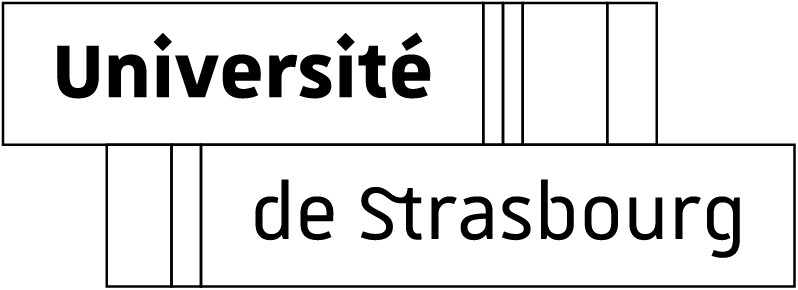
\includegraphics[width=0.22\paperwidth]{Images/Signature_Universite_Strasbourg_Unistra2_Transparent.png}}
 
    
      \begin{center}
      
      
      \vspace*{-1.2cm} %CHANGED
      
      {\Large \hspace{0.6cm} \textbf{UNIVERSITÉ DE STRASBOURG}}\\
      \vspace*{1.5cm} %CHANGED
      
      {\large \textbf{ÉCOLE DOCTORALE DE PHYSIQUE ET CHIMIE PHYSIQUE}}\\
      \textbf{Institut Pluridisciplinaire Hubert Curien (IPHC), UMR 7178}\\
      
      \vspace*{1.5cm} %CHANGED
      
      {\LARGE \textbf{TH\`{E}SE}}
      
      présentée par:
      
      \vspace*{0.3cm}
      
      {\Large \textbf{Mario Sessini}}
      
      soutenue le : \textbf{15 décembre 2023}
      
      
      \vspace*{0.5cm}
      
      pour obtenir le grade de: \textbf{Docteur de l'Université de Strasbourg}
      
      
      Discipline/Spécialité: Physique des particules élémentaires
      
      
      \vspace*{1cm}
      
      \fbox{
            \parbox{\textwidth}{\centering \LARGE \textbf{Recherche de violation de CP dans le couplage de Yukawa du lepton $\tau$ avec la méthode du vecteur polarimétrique dans les données du Run 2 de l'expérience CMS auprès du LHC}} %}
            %\centering
      }
      
      \end{center}
      
       \small
      
       \vspace*{0.2cm}
       %\vspace*{0.8cm}
      
       {\large \textbf{THÈSE dirigée par:}} %\\
      
       \vspace*{0.5cm}
      
       \setlength{\tabcolsep}{0.5cm}
       \begin{tabular}{ll}
             \textbf{Dr. Anne-Catherine LE BIHAN}          & Institut pluridisciplinaire Hubert Curien\\
       \end{tabular}
      
       \hrulefill
      
       \vspace*{0.5cm}
      
      
      % \begin{doublespace}
      
      
             {\large \textbf{RAPPORTEURS:}} %\\
      
             \vspace*{0.5cm}
      
             \setlength{\tabcolsep}{.5cm}
             \begin{tabular}{ll}
                   \textbf{Dr. Marco DELMASTRO} & Laboratoire d'Annecy de physique des particules\\
                   \textbf{Dr. Dirk ZERWAS} & Laboratoire de physique des 2 infinis Irène Joliot-Curie \\
             \end{tabular}
      
             \vspace*{0.8cm}
      
             {\large \textbf{EXAMINATEUR ET EXAMINATRICE:}} %\\
      
             \vspace*{0.5cm}
      
             \setlength{\tabcolsep}{0.5cm}
             \begin{tabular}{ll}
                  \textbf{Dr. Florian BEAUDETTE}          &  Laboratoire Leprince-Ringuet\\
                  \textbf{Dr. Isabelle RIPP-BAUDOT}          & Institut pluridisciplinaire Hubert Curien\\

             \end{tabular}
      
      % \end{doublespace}
      
      
      \end{titlepage}
    \cleardoublepage

    
    %\thispagestyle{empty}
    %\begin{flushright}
    %    \textit{\Large À ma mère.}
    %\end{flushright}

    \clearpage

    %%\thispagestyle{empty}
%\textbf{\huge Remerciements}
\addchap*{Remerciements}

La première personne que je souhaite remercier est tout naturellement ma directrice de thèse, Anne-Catherine Le Bihan. Ce fut (sans accent, j'ai compris maintenant) un réel plaisir de découvrir la recherche et de travailler à tes côtés pendant ces trois ans et demi. Merci pour ta patience sans limite, ton tempérament rassurant et ton écoute qui ont rendu cette thèse agréable même dans les moments compliqués. Bref, rien que pour toi : \textit{grazie mille !} \\

Je remercie tous les membres du groupe CMS de l'IPHC pour votre accueil depuis plusieurs années déjà. Merci tout particulièrement à Ulrich Goerlach qui m'a permis d'intégrer le groupe pour la première fois en 2018 pour y réaliser mon premier stage en physique des particules. Merci à Daniel Bloch pour ton encadrement de projet tuteuré de M1 sur la physique du $Z$ avec l'expérience DELPHI. Merci également à Éric Chabert pour tes cours de programmation de L3 (et tous les autres !) qui m'ont réconciliés avec le C++, et à tous les enseignants rencontrés à l'UNISTRA pendant mes études qui sont par la suite devenus mes collègues. Merci à Jérémy Andrea pour le partage du bureau du CERN, et comme il vaut mieux tard que jamais, désolé pour toutes les chaussettes sales qui y ont traîné. Enfin, merci à Saskia Falke pour ton aide précieuse et tes conseils, en particulier sur la fin de ma thèse. C'était aussi un plaisir de travailler et de discuter avec toi. \\

Tout ce travail est également le fruit de nombreux échanges et d'une collaboration avec les membres internationaux de CMS. En particulier, je souhaite remercier Andrea Cardini, Daniel Winterbottom, Konstantin Androsov, Aliaksei Raspiareza, David Colling, Michal Bluj, Vladimir Cherepanov et toutes les autres personnes brillantes avec qui j'ai eu l'occasion de travailler sur l'analyse Higgs CP ou au cours de mes EPR. \\

Je tiens également à remercier mes rapporteurs de thèse Marco Delmastro et Dirk Zerwas, mon examinateur Florian Beaudette et mon examinatrice Isabelle Ripp-Baudot. Merci d'avoir accepté de faire partie de mon jury, pour le temps consacré à la relecture de ma thèse, vos commentaires constructifs, et bien évidemment pour l'attribution du grade de docteur. \\

Il est maintenant temps de remercier toutes les personnes rencontrées à l'IPHC lors de cette thèse. Il serait difficile de ne pas commencer par toi Guillaume, encore doctorant lors de mon arrivée en stage et qui fait désormais partie des murs de l'IPHC. Merci pour ton aide à mes débuts sur l'analyse HCP et surtout merci pour ta joie de vivre débordante en toute circonstance, on t'adore. Merci à mes fidèles compagnons chevaliers de l'apocalypse : Océane, Dylan et Raphaël, dont l'union fut formée lors d'une CMS week très enneigée mais pas que. Océane, je te souhaite le meilleur pour la suite de ta thèse, $\tau$ ou tard tu finiras par y arriver. Dylan, merci pour ton humour gras et ton accent qui n'a jamais manqué de me rappeler d'où je venais. Raph, mon ange de la cabane du Bain Finkwiller, tu passeras le bonjour à ta voisine qui attend toujours à l'autre bout du fil. Je remercie également mon prof particulier de ping-pong Paul, et notre petit dernier, Gaël Cou... Ok j'arrête là, mais faire pleurer de rire AC, il fallait le faire. La liste est longue, mais je remercie évidemment tous les autres doctorants du laboratoire pour toutes nos pauses de midi agitées. \\

Puisque la fin de cette thèse marque également la fin de dix années d'études, je remercie tous mes amis présents depuis le début et ceux rencontrés en cours de route. Ugo, il faudrait sans doute écrire un roman pour raconter nos histoires partagées entre Lille, Toulouse, Strasbourg et partout ailleurs. Mais en quelques mots, merci d'avoir toujours été là et dans toutes les circonstances, les meilleures comme les pires. Merci à toute la bande strasbourgeoise : Konstantin, David, Justine, Thomas P., Iyas, Flavie, Bruno, Tim, Mathilde, Elise, Thomas M., Lison, Nolwenn, Tom... La liste est longue et incomplète mais vous avez tous fait de ces années une aventure inoubliable. Je pense également à mes plus fidèles camarades de fac : Lucas, Vincent et Vincent. Merci pour toutes ces années ensemble sponsorisées par la brasserie Meteor, la rue Munch en tremble encore. Merci également à mes amis vosgiens de longue date Nico, Mya, Bapt, Pierre F et tout particulièrement à François, Ornella, Patrick et Brigitte avec qui toute cette histoire de boson a démarré très fort en plein "confinage". François, Ornella, je vous souhaite tout le bonheur du monde pour votre mariage à venir. Enfin, Hélène, ta compagnie durant ces six derniers mois de thèse a fait de cette période un de mes plus beaux souvenirs. Pour tout ça, \textit{danke mit all meiner Liebe}, et que la suite soit encore meilleure. \\

Je me dois de terminer ces remerciements en dédiant quelques mots à tous mes proches, mon père, ma soeur, Brenda, Yassin, Jenna. Alexandra, tu es sans doute ma plus grande source d'inspiration et je te remercie pour toute l'attention que tu as su accorder à ton cher petit frère pendant toutes ces années. Merci à vous tous de m'avoir accompagné dans mes choix, de m'avoir soutenu sans relâche et de m'avoir fait grandir.  





	%\tableofcontents
 
    \clearpage
    \thispagestyle{empty}
    \hspace{1cm}


    
    %\addchap{Introduction}

À l'heure de l'écriture de cette thèse, plus de 11 années se sont écoulées depuis l'annonce de la découverte du boson de Higgs par les collaborations ATLAS et CMS au CERN le 4 juillet 2012 \cite{ATLASdiscovery,CMSdiscovery}. Sa découverte frappe notamment par la force avec laquelle elle vient affirmer le modèle théorique ayant prédit son existence près de 50 ans plus tôt \cite{BE,H}, et marque l'observation de la dernière particule élémentaire encore non observée prédite par le modèle standard de la physique des particules \cite{SM1,SM2,SM3}. Une vaste partie du programme de physique des hautes énergies est depuis consacré à la mesure de précision des propriétés du boson de Higgs. Dans cette thèse, ses propriétés de charge-parité (CP) à travers son couplage au lepton tau sont étudiées. À ce jour, l'étude des couplages de boson de Higgs aux bosons vecteurs se montre largement en faveur de l'hypothèse d'un boson de Higgs de nature purement scalaire tel que prédit par le modèle standard, et semble exclure son éventuelle nature pseudo-scalaire. En revanche, l'apparition d'une violation de CP est toujours possible au premier ordre dans les couplages de Yukawa, à travers un angle de mélange faisant intervenir à la fois une contribution scalaire et une contribution pseudo-scalaire au sein de ce dernier. Les premières mesures de cet angle de mélange dans plusieurs couplages \cite{ttH,Htautau} avec les données du Run 2 restent en accord avec l'hypothèse purement scalaire mais peuvent encore bénéficier, notamment dans le cas du couplage au lepton tau, de l'accroissement du volume de données produites dans les prochaines phases d'exploitation du \textit{Large Hadron Collider} (LHC) et d'une optimisation des méthodes de mesure. Toute découverte de violation de CP dans ce secteur constituerait alors une preuve tangible de l'existence de nouvelle physique, avec d'éventuelles implications en cosmologie dans le cadre de la baryogénèse électrofaible \cite{EWKbaryogenesis} en particulier. \\

Le premier chapitre de cette thèse sera dédié à une introduction historique des concepts de la physique moderne du début du $XX^e$ siècle et ayant donné lieu aux bases théoriques et expérimentales de la description du monde quantique. \\

Le second chapitre présentera ensuite le modèle standard de la physique des particules, en donnant des éléments théoriques de la structure des différentes interactions fondamentales qu'il décrit ainsi que du mécanisme de Brout-Englert-Higgs (BEH) ayant conduit à la brisure de symétrie électrofaible. \\

Dans le troisième chapitre, une présentation du CERN et de son histoire ainsi qu'une description du LHC et du détecteur CMS (\textit{Compact Muon Solenoid}) seront données. \\

Le quatrième chapitre contient une description des méthodes d'identification et de reconstruction des différentes particules et objets avec le détecteur CMS, et dans lequel un accent particulier est porté sur le lepton tau avec une étude sur les performances d'identification réalisée dans le cadre des EPR (\textit{Experimental Physics Responsabilities}) durant cette thèse. \\

Le cinquième chapitre est un état de l'art concernant la mesure expérimentale des propriétés du boson de Higgs et la recherche de violation de CP dans le secteur du Higgs, avec un regroupement des résultats de plusieurs analyses réalisées par la collaboration CMS. \\

Le sixième chapitre porte sur l'introduction des méthodes expérimentales de mesure de l'état CP du boson de Higgs employées au LHC. Parmi celles-ci se trouve la méthode du vecteur polarimétrique, dont les performances sont étudiées dans les canaux hadroniques $H\to\tau_h\tau_h$ et semi-leptoniques $H\to\mu\tau_h$. D'autres méthodes, propres à l'analyse de la structure CP du couplage de Yukawa du lepton tau sont également introduites avec notamment la méthode d'$embedding$ servant à la description du bruit de fond $Z\to\tau\tau$. Une étude des variables optimales de spin du lepton tau dans ces échantillons est aussi présentée. \\

Enfin, le septième chapitre présente le déroulement d'une mesure de l'angle de mélange CP dans le canal $a_1^{3pr}+\mu$ avec les données du Run 2. Dans cette analyse, la méthode du vecteur polarimétrique est comparée aux méthodes initiales avec une recherche d'optimisation de la sensibilité.
    %    \chapter{Introduction aux idées fondamentales}

                Le début du $XX^e$ siècle a vu naître avec lui la physique quantique, tirant son nom de la quantification des grandeurs observées dans un système physique au lieu des traditionnels continuums de la physique classique. En particulier, c'est l'introduction du quantum d'énergie par Max Planck en 1901 qui permettra de résoudre le problème de la \textit{catastrophe ultraviolette}, et qui conduira de nombreux physiciens tels que Niels Bohr, Albert Einstein ou encore Louis de Broglie à développer de nouveaux modèles dans le cadre de la \textit{théorie des quanta}. Sur cette base, des phénomènes comme la lumière alors décrits de façon purement ondulatoire trouveront une nature corpusculaire tandis que des objets tels que l'électron, décrits comme purement matériels, seront traités à la fois comme onde et particule. Ce concept est nommé la \textit{dualité onde-corpuscule} et servira de point de départ à la description des particules en mécanique quantique dans la première partie de ce chapitre. La seconde partie sera dédiée à une présentation des grandes idées de la mécanique quantique non-relativiste permettant de décrire l'évolution dans le temps d'un système quantique. Enfin les troisième et quatrième parties tenteront de présenter le cheminement des physiciens pour unifier la mécanique quantique à la relativité restreinte d'Albert Einstein \cite{Einstein1905} afin d'aboutir à la théorie quantique des champs, base essentielle de la physique des particules moderne. D'autres éléments permettant une introduction aux concepts fondamentaux traités dans cette thèse seront également présentés.
                
        \section{Description quantique des particules}
        
            Avec la découverte du photon, particule de lumière, la quantification de l'énergie est devenue indispensable pour la compréhension de certaines observations physiques comme les spectres d'absorption et d'émission des atomes qui présentent des raies fines et discrètes. Ce phénomène traduit la possibilité pour un atome d'absorber ou d'émettre des photons uniquement à des longueurs d'onde précises. Cela implique qu'un photon doit posséder une énergie correspondante à l'écart entre deux niveaux d'énergie $E_i$ et $E_j$ de l'atome pour être absorbé, et qu'un photon émit possédera une énergie égale à l'écart entre deux niveaux selon la formule : 
            
            \begin{equation}
                h\nu_{ij}=|E_i-E_j|,
            \end{equation}
            
        où $h\simeq6.62\times10^{-34}$ J.s est une constante appelée \textit{constante de Planck} et $\nu_{ij}$ est la fréquence d'un photon. En 1923, Louis de Broglie, inspiré par l'hypothèse de Max Planck, proposa  que \textit{<<les corpuscules matériels, tout comme les photons, peuvent avoir un aspect ondulatoire>>}. L'expérience de Davisson et Germer \cite{Germer1927} prouvera cette hypothèse en 1927 en montrant un comportement des électrons analogue à celui de la lumière par diffraction. Dès lors, on associera à tout corpuscule matériel d'énergie $E$ et d'impulsion $\vb{p}$ les relations de Planck-Einstein introduites pour le photon en 1924 après la découverte de \textit{l'effet Compton} \cite{Compton1923} :
            
            \begin{equation}
                \left\{
                    \begin{array}{ll}
                        E & = h\nu \\
                        \vb{p} & = \hbar\vb{k},
                    \end{array}
                \right.
            \end{equation}

            avec $\hbar=h/2\pi$ et $\vb{k}$ le vecteur d'onde, d'où découle l'expression d'une longueur d'onde d'après la relation de Louis de Broglie :
            
            \begin{equation}
                \lambda=\frac{2\pi}{|\vb{k}|}=\frac{h}{|\vb{p}|}.
            \end{equation}
            
        D'après ce résultat, la nature ondulatoire d'un corpuscule devient indissociable de sa nature matérielle. Cette relation relie aussi l'échelle d'énergie nécessaire à l'obtention d'une résolution suffisante permettant de sonder les constituants élémentaires de la matière.
        
        \section{Mécanique quantique non-relativiste}
        
         D'après les éléments apportés par le paragraphe précédent, une particule libre peut être décrite comme un état quantique $\ket{\psi(t)}$ dépendant du temps $t$, à travers un objet de nature ondulatoire appelé fonction d'onde et noté $\psi(\vb{x},t)$, correspondant à la projection de l'état quantique $\ket{\psi(t)}$ sur une base $\ket{\vb{x}}$ de l'espace :
        
        \begin{equation}
            \psi(\vb{x},t)=\bra{\vb{x}}\ket{\psi(t)}\propto Ne^{i(\vb{p}.\vb{x}-Et)},
            \label{onde}
        \end{equation}
            
        où $N$ est une constante de normalisation. La définition de cet objet veut que toute information sur un état quantique soit contenue dans sa fonction d'onde. Ainsi la première conséquence sera que la notion de trajectoire telle qu'elle est entendue au sens classique doit être abandonnée au profit d'une amplitude de probabilité de présence en un point donné de l'espace. D'autre part, l'accès à certaines grandeurs comme l'impulsion ou l'énergie d'une particule se fait à travers des opérateurs $\hat{A}$ agissant sur la fonction d'onde de manière à retourner une grandeur $a$ :
        
        \begin{equation}
            \hat{A}\psi(\vb{x},t)=a\psi(\vb{x},t).
        \end{equation}
        
        On dit alors que $\psi(\vb{x},t)$ est un état propre de l'opérateur $\hat{A}$, de valeur propre $a$, et cette grandeur correspondra à une observable physique lorsque sa valeur sera purement réelle. Dans le cas de l'impulsion et de l'énergie, il est possible d'introduire respectivement les opérateurs $\hat{\vb{p}}$ et $\hat{E}$ :
        
        \begin{equation}
            \hat{\vb{p}} = -i\grad \quad \mbox{et } \quad
            \hat{E} = i\pderivative{t},
            \label{ops}
        \end{equation}

        de sorte à obtenir en utilisant l'expression \ref{onde} de la fonction d'onde :
        
        \begin{equation}
            \left\{
                \begin{array}{ll}
                    \hat{\vb{p}}\psi(\vb{x},t)=\vb{p}\psi(\vb{x},t) \\
                    \hat{E}\psi(\vb{x},t)=E\psi(\vb{x},t).
                \end{array}
            \right.
        \end{equation}       
        
        Par analogie à la mécanique classique, où l'énergie totale d'un système est donnée par la somme de l'énergie cinétique $T$ et de l'énergie potentielle $V$ à travers l'Hamiltonien $H=T+V$, il est possible de définir un opérateur Hamiltonien quantique pour une particule de masse $m$ :
        
        \begin{equation}
                \hat{H}=\frac{\hat{\vb{p}}^2}{2m}+\hat{V}=-\frac{1}{2m}\laplacian + \hat{V}.
        \end{equation}
        
        L'application de l'opérateur Hamiltonien sur la fonction d'onde donne lieu à la célèbre équation de Schrödinger dépendante du temps qui permet de décrire à tout instant l'évolution de $\psi(\vb{x},t)$ :
        
        \begin{equation}
        \boxed{
            i\pdv{\psi(\vb{x},t)}{t}=\hat{H}\psi(\vb{x},t).
        }
        \end{equation}
        
        D'après l'opérateur énergie introduit plus tôt, on remarque alors que si la fonction d'onde $\psi_i(\vb{x},t)$ est un état propre de l'opérateur Hamiltonien on obtient naturellement :
        
        \begin{equation}
            \hat{H}\psi_i(\vb{x},t)=E_i\psi_i(\vb{x},t).
        \end{equation}
        
        Comme mentionné plus tôt, la fonction d'onde contient toutes les informations d'un système quantique et peut ainsi être utilisée pour définir une densité de probabilité de présence. Si la valeur $\psi^*(\vb{x},t)\psi(\vb{x},t)\dd[3]{\vb{x}}$ est associée à la probabilité de trouver une particule dans le volume infinitésimal $\dd[3]{\vb{x}}$, alors cette densité de probabilité est définie selon :
        
        \begin{equation}
            \rho(\vb{x},t)=\psi^*(\vb{x},t)\psi(\vb{x},t).
        \end{equation}
        
        L'évolution temporelle de $\rho(\vb{x},t)$ permet également de définir un courant de probabilité $\vb{j}(\vb{x},t)$, en considérant que si la densité de probabilité au sein d'un volume $V$ varie alors il existe un courant de probabilité à travers la surface $\vb{S}$ des parois de ce volume :
        
        \begin{equation}
            \pdv{t}\int_V\rho\dd{V}=-\int_S\vb{j}\vdot \dd{\vb{S}}=-\int_V\grad\vdot\vb{j}\dd{V}.
            \label{div}
        \end{equation}

        Le dernier terme de \ref{div} est obtenu grâce au théorème de la divergence, et cette équation étant valide pour tout volume arbitraire il est possible d'écrire l'équation de continuité suivante :

        \begin{equation}
            \grad\vdot\vb{j}+\pdv{\rho}{t}=0.
        \end{equation}

        L'équation de Schrödinger pour une particule libre, c'est à dire sans terme de potentiel, permet de définir la forme du courant $\vb{j}$ en écrivant :

        \begin{equation*}
        \begin{split}
        i\pdv{\rho}{t} & =i\pdv{t}(\large\psi^*\psi) \\
         & = i\Biggl(\pdv{\psi^*}{t}\psi + \psi^*\pdv{\psi}{t}\Biggr) \\
         & = -\frac{1}{2m}(\psi^*\laplacian\psi-\psi\laplacian\psi^*) \\
         & = -\frac{1}{2m}\grad\vdot(\psi^*\grad\psi-\psi\grad\psi^*) \\
        \end{split}
        \end{equation*}

        Soit :

        \begin{equation*}
            \vb{j} = \frac{1}{2im}(\psi^*\grad\psi-\psi\grad\psi^*). \\
        \end{equation*}

        En résumé, la densité de probabilité et le courant de probabilité exprimé en fonction de l'expression de la fonction d'onde \ref{onde} peuvent s'écrire :

        \begin{equation}
            \boxed{
            \rho=\psi^*\psi \quad \mbox{et} \quad \vb{j}=|N|^2\frac{\vb{p}}{m}.
            }
        \end{equation}
        
        Pour tout opérateurs $\hat{A}$ et $\hat{B}$ il également possible de définir une relation de commutation 
        
        \begin{equation}
            [\hat{A},\hat{B}]=\hat{A}\hat{B}-\hat{B}\hat{A},
        \end{equation}
        
        pour laquelle on dira que $\hat{A}$ et $\hat{B}$ commutent lorsque $[\hat{A},\hat{B}]=0$, et ne commutent pas le cas échéant. Cette relation a de fortes implications en mécanique quantique, puisqu'elle détermine la possibilité ou non de mesurer simultanément deux observables d'un état quantique. À titre d'exemple, la non-commutation des opérateurs de position et d'impulsion permet d'illustrer le principe d'incertitude de Heisenberg selon lequel il est impossible de connaître simultanément de façon précise la vitesse et la position d'une particule. 
    
        \section{Vers une théorie quantique relativiste}
        \label{verslarelat}
        
         Le début du $XX^e$ siècle marque également la naissance de la relativité restreinte par Albert Einstein permettant de décrire des systèmes ayant une vitesse non négligeable devant celle de la lumière. Selon cette théorie, la vitesse de la lumière est une constante dans tout référentiel galiléen et implique qu'une cause entraîne toujours un effet dans un délai minimal nécessaire à la lumière pour parcourir la distance entre la cause et l'effet dans ce qui est nommé \textit{principe de causalité}. Les objets relativistes sont quant à eux décrits dans un espace à quatre dimensions appelé \textit{espace-temps de Minkowski} grâce à des quadrivecteurs dans lesquels le temps devient une composante à part entière aux côtés des trois coordonnées spatiales $(x,y,z)$ de l'espace Euclidien. Ces objets peuvent également subir des transformations de coordonnées grâce aux transformations de Lorentz, à l'origine des effets de dilatation temporelle de la relativité restreinte. Certaines quantités telle que la masse en physique des particules sont inchangées par ces transformations, elles sont alors \textit{invariantes de Lorentz}. L'équation de Schrödinger, qui comporte un terme de dérivation temporelle au premier ordre tandis que le terme de dérivation spatiale est au second, n'est pas invariante de Lorentz et est donc incompatible avec la relativité restreinte d'Einstein. En revanche des systèmes physiques tels que l'atome d'hydrogène représenté par un électron plongé dans un potentiel coulombien, induit par le proton, ne peuvent être décrits de manière complète sans inclure des effets relativistes. Les premiers travaux pour concilier relativité et mécanique quantique seront réalisés indépendamment par Oskar Klein et Walter Gordon en 1926. En effet, il est possible à partir de la forme relativiste de la relation entre énergie et impulsion 
        
        \begin{equation}
            E^2=\vb{p}^2+m^2,
            \label{Eprelation}
        \end{equation}

        de construire une équation relativiste en remplaçant chaque terme par un opérateur tel qu'introduit dans l'équation \ref{ops} et agissant sur une fonction d'onde $\psi(\vb{x},t)$. On obtient alors l'équation de Klein-Gordon :
        
        \begin{equation}
        \boxed{
            (\partial^{\mu}\partial_{\mu}+m^2)\psi(\vb{x},t)=0
        ,}
        \label{KG}
        \end{equation}
        
        avec $$\partial^{\mu}\partial_{\mu}\equiv\pdv[2]{t}-\pdv[2]{x}-\pdv[2]{y}-\pdv[2]{z}.$$
        
        Comme pour l'équation de Schrödinger, il est possible de définir une densité et un courant de probabilité :

        \begin{equation}
        \boxed{
            \rho=2|N|^2E \quad \mbox{et} \quad \vb{j}=2|N|^2\vb{p}.
        }
        \end{equation}
        
        Malgré une réussite apparente de joindre la relativité d'Einstein à la mécanique quantique, cette équation apporte également une densité de probabilité de présence négative dépourvue de sens physique aux solutions d'énergie négative. Ces résultats ont amené Paul Dirac en 1928 à rechercher à son tour une équation relativiste, qui face aux conclusions précédentes, devra être dérivée d'ordre un à la fois d'espace et de temps et de forme générale :
        
        \begin{equation}
            \hat{E}\psi=(\vb*{\alpha}\vdot\vb{\hat{p}}+\beta m)\psi.
            \label{dirac1}
        \end{equation}
        
        Il est également nécessaire, pour décrire correctement des objets relativistes, que les solutions de cette équation obéissent à la relation relativiste entre l'énergie et l'impulsion \ref{Eprelation}. Ainsi l'équation proposée par Dirac doit être compatible avec l'équation de Klein-Gordon. Il est alors possible de montrer à partir de cette condition que les objets $\vb*{\alpha}=(\alpha_x, \alpha_y, \alpha_z)$ et $\beta$ constituent un ensemble de  quatre matrices de dimension quatre agissant sur une fonction d'onde particulière à quatre composantes appelée \textit{spineur de Dirac} :
  
        \[
            \psi = 
            \begin{pmatrix}
                \psi_1 \\
                \psi_2 \\
                \psi_3 \\
                \psi_4
            \end{pmatrix}
        ,\]
        
        et que la forme la plus simple pour $\vb*{\alpha}$ et $\beta$ se retrouve dans la représentation de Dirac-Pauli avec :
        
        \[
            \alpha_i = 
            \mqty(0 && \sigma_i \\ \sigma_i && 0)
            \quad
            \mbox{ et }
            \quad
            \beta = 
            \mqty(I && 0 \\ 0 && -I)
        ,\]
        
        où $i=x,y,z$, avec $\sigma_i$ représentant chacune une des trois matrices de Pauli :
        
        \[
            \sigma_x = 
            \mqty(0 && 1 \\ 1 && 0)
            \mbox{, }
            \quad
            \sigma_y = 
            \mqty(0 && -i \\ i && 0)
            \mbox{, }
            \quad
            \sigma_z = 
            \mqty(1 && 0 \\ 0 && -1)
        \]
        
        et où $I$ est la matrice unité de dimension deux. \\
        
        On retrouvera plus souvent l'équation de Dirac sous sa forme dite covariante :
        
        \begin{equation}
        \boxed{
            (i\gamma^{\mu}\partial_{\mu}-m)\psi(\vb{x},t)=0,
        }
        \label{dirac2}
        \end{equation}
        
        avec
        
        $$
        \begin{array}{ll}
            \gamma^{\mu}\partial_{\mu} & \equiv\gamma^0\pdv{t}+\gamma^1\pdv{x}+\gamma^2\pdv{y}+\gamma^3\pdv{z} \\
            & \\
            & \equiv\beta\pdv{t}+\beta\sigma_x\pdv{x}+\beta\sigma_y\pdv{y}+\beta\sigma_z\pdv{z}.
        \end{array}
        $$

        Finalement l'expression de la densité et du courant de probabilité est donnée par :

        \begin{equation}
            \boxed{
            \rho=\psi^{\dag}\psi \quad \mbox{et} \quad \vb{j}=\psi^{\dag}\vb*{\alpha}\psi,
            }
        \label{probdirac}
        \end{equation}

        où $\psi^{\dag}=(\psi^*)^T$ est le conjugué hermitien de $\psi$. \\
        
        Bien que cette nouvelle équation semble effectivement compatible avec la relativité restreinte, elle autorise également l'énergie de l'électron à prendre des valeurs négatives dont les physiciens peineront à justifier l'existence. Paul Dirac a alors tenté dans un premier temps de décrire l'existence d'une $\textit{mer}$ constituée d'électrons virtuels occupants de manière discrète tous les niveaux d'énergie allant de l'infini négatif à une valeur maximale appelée $\textit{niveau de la mer}$, où un électron quittant cette mer laisserait derrière lui un <<trou>> dont l'énergie serait positive. Devant les incohérences de cette théorie et après une tentative échouée d'établir un lien avec le proton, il postulera finalement en 1931 l'existence du positron, jumeau d'anti-matière de l'électron, découvert l'année suivante en chambre à brouillard par Carl David Anderson \cite{Anderson1932}. \\
        
        Il est également intéressant de noter au sujet de l'équation de Dirac sa capacité à intégrer naturellement dans son formalisme les degrés de liberté supplémentaires du spin de l'électron, notion prédite quelques années plus tôt. En effet, certaines observations physiques du début du siècle telles que la levée de dégénérescence des niveaux d'énergie d'un atome plongé dans un champ magnétique et leur structure hyperfine, ou encore les résultats de l'\textit{expérience de Stern et Gerlach} \cite{Gerlach1922}, ont trouvé une explication lors de l'introduction du spin en 1925 par Samuel Goudsmit et George Uhlenbeck \cite{Uhlenbeck1925}. Bien que d'abord vu comme une rotation de l'électron sur lui-même, il s'agit en réalité d'un degré de liberté supplémentaire sans équivalent classique davantage lié à des propriétés magnétiques que mécaniques. Le spin de l'électron a par la suite été formalisé par Wolfgang Pauli en 1927 sous forme d'opérateurs agissant sur la fonction d'onde et constitués des trois matrices de Pauli présentées plus tôt. Dans ce formalisme, l'opérateur de spin $\hat{S}$ est introduit comme un opérateur vectoriel composé des trois composantes spatiales $\hat{S_x}, \hat{S_y}, \hat{S_z}$ ne commutant pas entre elles mais qui commutent individuellement avec $\hat{S}$. En d'autres termes, la mécanique quantique autorise uniquement la mesure simultanée du spin total d'une particule et de sa projection sur une des trois directions de l'espace, la connaissance de sa valeur dans les autres directions étant alors perdue.
        
        \section{L'interaction par la théorie des champs}
        \label{sectionQFT}
        
        Du côté de la physique classique, la théorie du champ électromagnétique découlant directement des équations de Maxwell était déjà une excellente intégration de la relativité restreinte dans un modèle physique \cite{Maxwell}. Elle permet notamment de décrire avec succès les interactions de la matière chargée et le comportement du rayonnement électromagnétique. Dans une première tentative de quantification de l'électromagnétisme, Dirac tenta de décrire de manière séparée la matière chargée par le formalisme ondulatoire de Schrödinger et le rayonnement par la propagation d'une onde quantifiée associée au photon. De ce point de vue, la mécanique quantique est alors incapable d'unir la vision d'une particule chargée a priori éternelle à celle d'un photon éphémère capable d'être créé par émission puis annihilé par absorption. Ce problème se verra résolu de manière naturelle, mais non sans difficulté, par le développement pendant plus de 10 ans de la théorie quantique des champs (QFT, \textit{Quantum Field Theory}) selon laquelle toute particule peut être associée à un champ. Dans ce nouveau formalisme les opérateurs de création et d'annihilation, dénotés $\hat{a}^{\dag}_k$ et $\hat{a}_k$ respectivement, sont introduits dans le but d'agir sur un champ donné afin de créer ou annihiler un quanta d'énergie représenté par une particule associée à ce champ. Dans ce cadre, les solutions de l'équation de Klein-Gordon \ref{KG} représentent des champs scalaires qui, une fois soumis à l'action de l'opérateur de création, donnent naissance à des particules sans spin appelées bosons scalaires, tandis que les solutions de l'équation de Dirac \ref{dirac1} donnent naissance à des fermions de spin $\sfrac{1}{2}$ tels que l'électron. D'autres champs de type vectoriels sont quant à eux capables de produire des particules de spin 1 appelées bosons vecteurs à trois degrés de liberté de spin, soit un de plus que les fermions, à l'exception du photon qui possède seulement deux états de polarisation car non massif. \\
        
        Il reste toutefois à décrire la façon dont les différentes particules sont susceptibles d'interagir entre elles afin de produire des processus physiques observables expérimentalement. La mécanique quantique décrit la transition d'un état initial vers un état final dans le cadre de la théorie des perturbations, selon laquelle une particule se diffuse dans un potentiel extérieur en échangeant une partie de son impulsion. Cette vision est néanmoins incomplète sur deux aspects fondamentaux : elle fait intervenir le concept d'interaction sans fournir la description d'un quelconque médiateur, et viole la causalité dans le sens où si une autre particule est ajoutée au système son potentiel prendrait effet dans la perturbation partout et instantanément. Dans le cadre de la QFT ces aspects sont couverts en donnant à des particules porteuses de force le rôle de médiatrices, ce qui ne viole pas la causalité puisque ces échanges sont limités par la vitesse de ces particules nécessairement inférieure à celle de la lumière. Prenons le cas d'une interaction entre deux électrons notés $e_1$ et $e_2$ durant laquelle se produit un transfert d'impulsion par échange d'une particule $X$. Il serait possible a priori de décrire ce processus de sorte que $e_1$ soit responsable de l'émission de $X$ à un instant $t_1$ qui sera ensuite absorbée par $e_2$ à un instant ultérieur $t_2$, ou au contraire que $e_2$ soit responsable de l'émission à $t_1$, et $e_1$ de l'absorption à $t_2$. Ces deux modes d'action peuvent en réalité d'un point de vue mathématique être sommés et condensés en un seul diagramme appelé \textit{diagramme de Feynman} (fig.\ref{sumfeynman}). Inventés par Richard Feynman dans les années 1940, ces diagrammes sont une représentation graphique qui au-delà de leur aspect simple contiennent toute la complexité calculatoire de la théorie quantique des champs. Ils permettent notamment d'illustrer la somme des différentes  chronologies d'un processus physique comme vu dans l'exemple précédent, ainsi que toutes les combinaisons de spin des particules impliquées. \\
        
        \begin{figure}
            \centering
            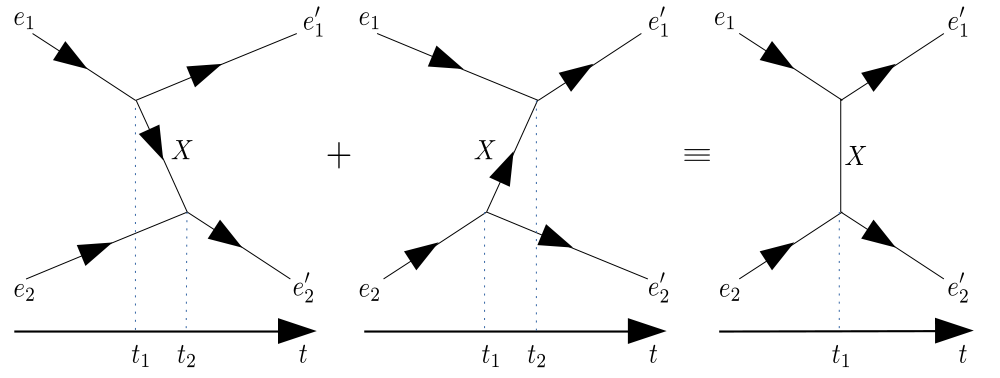
\includegraphics[scale=0.28]{Chapitre1/Images/sumfeynman.png} 
            \caption{Différentes chronologies de l'interaction entre $e_1$ et $e_2$ et représentation du diagramme de Feynman associé.}
        \label{sumfeynman}
        \end{figure}
        
        La figure \ref{bhabha} illustre un exemple réel d'interaction entre un électron et un positron appelée diffusion Bhabha. Ce processus fait intervenir l'échange d'un photon entre une paire électron/positron (e$^+$/e$^-$) dans le cadre de la théorie quantique de l'électromagnétisme (QED, \textit{Quantum Electrodynamics}), première théorie basée sur la QFT datant de la fin des années 1940. On peut alors écrire le diagramme de Feynman associé de deux façons, la première étant une annihilation donnant naissance à une nouvelle paire (voie $s$), et la seconde une diffusion élastique classique (voie $t$). \\
        
        \begin{figure}
            \centering
            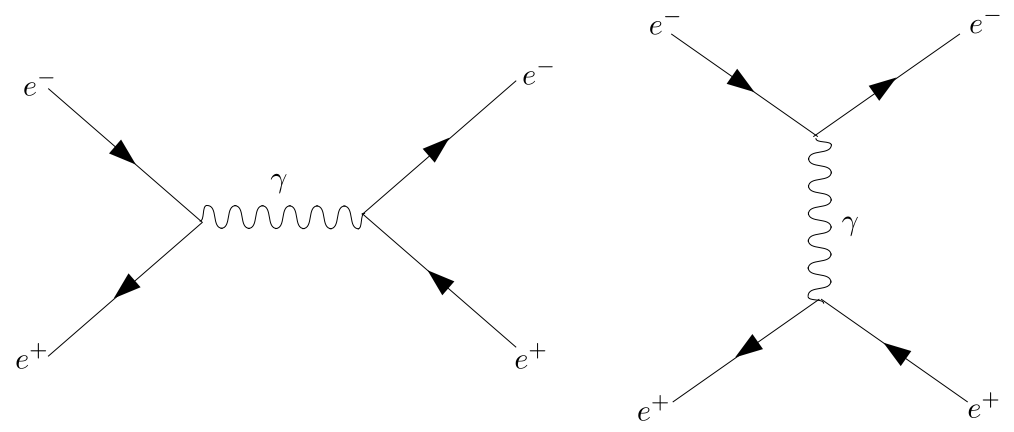
\includegraphics[scale=0.28]{Chapitre1/Images/bhabha.png} 
            \caption{Diffusion Bhabha en voie $s$ (gauche) et en voie $t$ (droite).}
        \label{bhabha}
        \end{figure}
        
        \section{Symétries et lois de conservation}

         En mécanique classique, il est facile de retrouver la seconde loi de Newton à partir du Lagrangien pour une particule classique se déplaçant selon l'axe $x$, défini comme la différence entre l'énergie cinétique et l'énergie potentielle :

        $$L=T-V=\frac{1}{2}m\dot{x}^2-V(x).$$

        En appliquant les équations d'Euler-Lagrange

        \begin{equation}
            \dv{t}\Biggl(\pdv{L}{\dot q_i}\Biggr)-\pdv{L}{q_i} = 0,
        \end{equation}

        on trouve alors pour la coordonnée généralisée $q_i=x$ :
        \begin{equation*}
        \begin{split}
            \quad \dv{t}\Biggl(\pdv{L}{\dot x}\Biggr)-\pdv{L}{x} & = \dv{t}m\dot x + \pdv{V}{x} \\
            & = 0.
        \end{split}
        \end{equation*}

        Soit finalement

        \begin{equation}
            m\ddot x = -\pdv{V(x)}{x}.
        \end{equation}

        Dans le cas d'une particule libre, c'est-à-dire lorsque $V(x)=0$, le Lagrangien ne contient plus de dépendance spatiale. Il comporte alors désormais une symétrie et devient invariant par transformation de translation de la coordonnée $x$ :

        $$x\rightarrow x' = x+\var x$$.

        Selon le théorème d'Emmy Noether introduit en 1915 \cite{Noether1918}, la présence d'une symétrie au sein du Lagrangien entraîne l'existence d'une grandeur conservée au sein du système. Dans le cas où cette symétrie est une invariance par translation, il est possible de montrer que l'impulsion du système est conservée, illustrant notamment la 3ème loi de Newton. \\

        Par analogie, le formalisme de la mécanique lagrangienne s'inscrit naturellement au sein de la QFT afin de dériver les équations du mouvement satisfaites par les champs introduits plus tôt. La notion de Lagrangien pour un système discret peut être étendue à celle d'un système continu en introduisant une densité de Lagrangien et en remplaçant la dépendance aux coordonnées généralisées $(q_i,\dot q_i)$ par les champs $\phi_i$ et leurs dérivées selon les quatre dimensions de l'espace-temps $\partial_{\mu}\phi_i$ :

        $$L\Bigl(q_i,\dot q_i\Bigr)\rightarrow\mathcal{L}\Bigl(\phi_i,\partial_{\mu}\phi_i\Bigr),$$

        définie telle que 
        
        $$L\Bigl(\phi_i,\partial_{\mu}\phi_i\Bigr)=\int\mathcal{L}\Bigl(\phi_i,\partial_{\mu}\phi_i\Bigr)\dd[3]{x}.$$

        Enfin, l'action $S$ d'un système peut être définie comme l'intégrale temporelle du Lagrangien :

        $$S=\int L\Bigl(\phi_i,\partial_{\mu}\phi_i\Bigr)\dd{t} = \int\mathcal{L}\Bigl(\phi_i,\partial_{\mu}\phi_i\Bigr)\dd[4]{x},$$

        et selon le principe de moindre action, stipulant que l'action est stationnaire, il est possible de définir les équations d'Euler-Lagrange pour $\phi_i$ :

        \begin{equation}
        \boxed{
            \fdv{S}{\phi_i}=\pdv{\mathcal{L}}{\phi_i}-\partial_{\mu}\Biggl(\pdv{\mathcal{L}}{(\partial_{\mu}\phi_i)}\Biggr)=0.
        }
        \label{action}
        \end{equation}

        Prenons maintenant l'exemple de la densité de Lagrangien pour un spineur de Dirac libre en introduisant le spineur de Dirac adjoint $\overline{\psi}\equiv\psi^{\dag}\gamma^0$ :

        \begin{equation}
            \mathcal{L}_{\mbox{\tiny Dirac}}=\overline{\psi}\bigl(i\slashed\partial-m\bigr)\psi,
        \label{Ldirac}
        \end{equation}

        avec $\slashed \partial = \gamma^{\mu}\partial_{\mu}$. \\

        Il serait notamment possible de montrer que l'injection de $\mathcal{L}_{\mbox{\tiny Dirac}}$ dans l'équation \ref{action} permet de retrouver l'équation de Dirac telle que formulée dans l'équation \ref{dirac2}. Il est également possible de montrer que le Lagrangien de Dirac est invariant sous une transformation globale de $\psi$ du groupe de symétrie U($1$) telle que 

        $$\psi\rightarrow\psi'=e^{i\theta}\psi.$$

        Selon le théorème de Noether une nouvelle fois, cette symétrie implique l'existence d'une grandeur conservée qui peut être montrée comme étant le quadrivecteur constitué de la densité et du courant de probabilité définis dans \ref{probdirac} : 

        \begin{equation}
        \boxed{
            j^{\mu}=(\rho,\vb{j})=\overline{\psi}\gamma^{\mu}\psi. 
        }
        \label{fermioncurrent}
        \end{equation}

        \vspace{10pt}
        En résumé, les physiciens sont parvenus en près de 50 ans à mettre au point des outils permettant d'étudier et de comprendre le fonctionnement de l'infiniment petit. Ces recherches ont notamment permis de nombreuses découvertes qui représentent aujourd'hui les fondements de la physique des particules moderne. La théorie quantique de l'électromagnétisme, aboutie entre 1946 et 1950 par R. Feynman, J. Schwinger et S. Tomonaga, est encore aujourd'hui une théorie dont la précision des prédictions reste inégalée. Cette période marque aussi le commencement de nombreux travaux dans le but de développer des nouveaux modèles dans le cadre de la théorie quantique des champs qui constitueront les prémices du modèle standard de la physique des particules. Le chapitre suivant sera consacré à la mise en forme et à l'assemblage des différentes théories qui le constituent, en s'appuyant sur des principes de symétrie tels qu'ils ont été présentés dans la dernière partie de ce chapitre.
    %    \chapter{Le modèle standard de la physique des particules}

    En physique moderne, l'Univers est gouverné par quatre interactions fondamentales, à savoir l'interaction électromagnétique, l'interaction faible, l'interaction forte et l'interaction gravitationelle. Le modèle standard (MS) \cite{SM1,SM2,SM3} est le modèle regroupant les théories quantiques capables de décrire ces interactions, à l'exception de la gravitation qui à ce jour est décrite par la théorie de la relativité générale d'Albert Einstein et ne possède pas de formulation à l'échelle microscopique. Ainsi le MS fournit une description des \textit{particules élémentaires} et de leurs interactions à travers les outils de la théorie quantique des champs. Après la formulation de la théorie quantique de l'électromagnétisme autour de 1950, les années suivantes ont donné lieu au développement du modèle pour lui donner sa forme actuelle au milieu des années 1970. Depuis, chaque particule prédite au sein du MS a été observée expérimentalement, la dernière découverte étant celle du boson de Higgs en 2012.

    \section{Classification des particules}

    Le modèle standard de la physique des particules comporte deux grandes familles de particules. La première est celle des fermions qui regroupe douze particules de spin $\sfrac{1}{2}$ constitutives de la matière et associées à des champs de Dirac. Elle est elle-même scindée en deux familles avec d'un côté six saveurs de quarks, dont les deux plus légères composent majoritairement les protons et neutrons, et de l'autre six saveurs de leptons dont le plus connu est l'électron. On cite également parmi les fermions l'existence de trois générations contenant chacune deux quarks, dont un de charge électrique $\sfrac{+2}{3}$ et l'autre de charge électrique $\sfrac{-1}{3}$, et deux leptons dont un neutre et un de charge électrique -$1$. La première génération est celle qui forme toute la matière stable avec les quarks up et down, le neutrino électronique et l'électron. Les deux suivantes sont constituées de particules instables se désintégrant rapidement en particules de génération inférieure. À chacune de ces douze particules est également associée une antiparticule constituante de l'antimatière, semblable en tout point à sa jumelle de matière mais avec des nombres quantiques tels que la charge électrique opposés. La symétrie gouvernant l'équité des interactions entre matière et antimatière est appelée symétrie de \textit{charge-parité} (CP) et sera discutée dans le chapitre \ref{violCP}.

    \begin{figure}
    \centering
        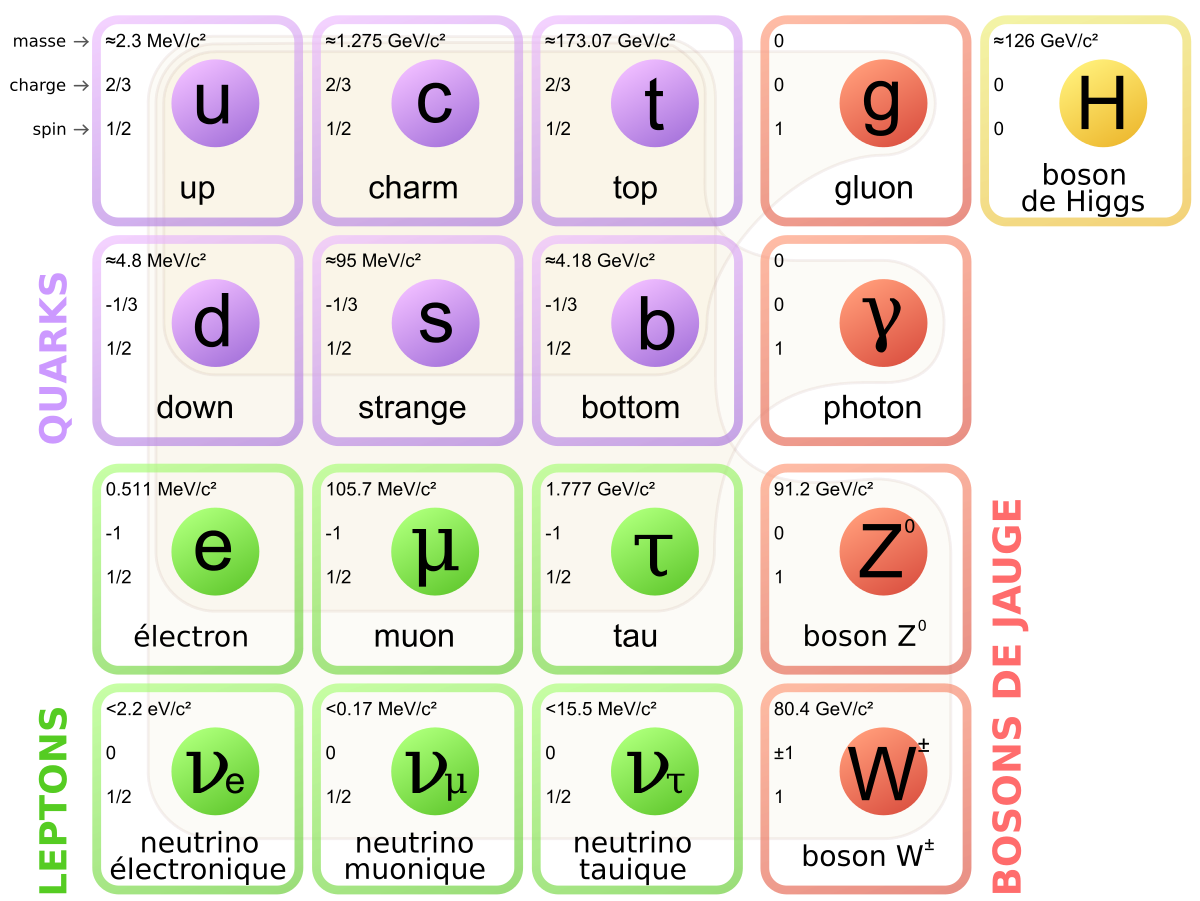
\includegraphics[scale=0.22]{Chapitre2/Images/MS.png} 
        \caption{Représentation graphique des particules du modèle standard. Les douze fermions sont constitués des six quarks (violet) et des six leptons (vert). Chacune des trois générations est formée par une colonne constituée de deux quarks et deux leptons. Les bosons de jauge sont présentés en rouge et le boson de Higgs en jaune \cite{particles}.}
    \label{MS}
    \end{figure}

    La seconde grande famille est formée par les bosons de jauge, ou bosons vecteurs, particules de spin $1$ porteuses de force telles qu'introduites dans le paragraphe \ref{sectionQFT} et associées à des champs vectoriels. Parmi celles-ci se trouvent le photon, médiateur de l'interaction électromagnétique, les bosons $W^{\pm}$ et $Z^0$, médiateurs de l'interaction faible et enfin les gluons, médiateurs de l'interaction forte. Finalement, le boson de Higgs est la seule particule élémentaire du modèle standard de spin $0$ et associée à un champ scalaire. Il n'est donc pas une particule médiatrice au sens propre du terme mais entre en jeu dans un mécanisme explicité dans le paragraphe \ref{higgsmeca} à travers lequel les autres particules élémentaires acquièrent une masse. 
    
    \section{Classification des interactions}

    Ce paragraphe est dédié à l'introduction des trois forces fondamentales décrites par le modèle standard. Dans un premier temps, une description de la nature de l'interaction sera donnée ainsi que quelques exemples concrets de manifestations physiques de ces dernières. Par la suite, chaque Lagrangien sera présenté ainsi que les symétries qui lui sont associées afin de comprendre la nature de chaque interaction à travers quelques diagrammes de Feynman.

        \subsection{Interaction électromagnétique}

        L'interaction électromagnétique est sans doute l'interaction dont les manifestations physiques sont les plus évidentes. Son boson de jauge, le photon, est la particule associée au champ électromagnétique et constitue donc par définition les ondes électromagnétiques quelle que soit leur fréquence, et de cette façon la lumière visible. Dans le cadre de la théorie quantique des champs, l'interaction électromagnétique est capable d'agir sur toute particule élémentaire portant une charge électrique et fait intervenir entre ces dernières l'échange d'un photon sans masse et de charge électrique nulle. \\

        Le Lagrangien de la QED noté $\mathcal{L}_{\tiny QED}$ peut être construit à partir du Lagrangien de Dirac $\mathcal{L}_{\tiny Dirac}$ introduit dans l'équation \ref{Ldirac}. En tentant d'appliquer à un spineur de Dirac libre $\psi$ une transformation du groupe de symétrie U($1$) cette fois locale et non plus globale :

        \begin{equation}
            \psi\rightarrow\psi'=e^{i\chi(\vb{x},t)}\psi,
        \label{localU1}
        \end{equation}

        $\mathcal{L}_{\tiny Dirac}$ se transforme de la façon suivante :

        \begin{equation*}
            \boxed{\overline{\psi}\bigl(i\gamma^{\mu}\partial_{\mu}-m\bigr)\psi}\rightarrow\boxed{\overline{\psi}\bigl(i\gamma^{\mu}(\partial_{\mu}+i\partial_{\mu}\chi)-m\bigr)\psi\ne\mathcal{L}_{\tiny Dirac}}
        \end{equation*}

        et perd ainsi son invariance. Cette dernière peut être conservée en introduisant un \textit{champ de jauge} noté $A_{\mu}$ se transformant selon $A_{\mu}\rightarrow A'_{\mu}=A_{\mu}-\frac{1}{q}\partial_{\mu}\chi$. Le nouveau Lagrangien invariant s'écrit ainsi :

        \begin{equation}
            \mathcal{L}=\overline{\psi}\bigl(i\gamma^{\mu}(\partial_{\mu}+iqA_{\mu})-m\bigr)\psi.
        \end{equation}

        On remarque alors que la conservation de la symétrie du Lagrangien sous une transformation de U($1$) impose l'introduction d'un champ de jauge dont la nature vectorielle implique l'existence d'un boson de jauge de spin $1$ sans masse, défini comme le photon. De plus, le théorème de Noether indique la conservation de la grandeur $q$ associée à la charge électrique. D'ores et déjà ce Lagrangien peut être développé afin d'exposer la nature des différents termes qui le composent :

        \begin{equation}
            \boxed{\mathcal{L}=
            i\overline{\psi}\gamma^{\mu}\partial_{\mu}\psi
            -m\overline{\psi}\psi
            -q\overline{\psi}\gamma^{\mu}A_{\mu}\psi}
        \end{equation}

        \begin{enumerate}
            \item[$\bullet$] $i\overline{\psi}\gamma^{\mu}\partial_{\mu}\psi$ : terme cinématique associé aux fermions,
            \item[$\bullet$] $m\overline{\psi}\psi$ : terme de masse associé aux fermions,
            \item[$\bullet$] $q\overline{\psi}\gamma^{\mu}A_{\mu}\psi$ : interaction entre fermions et champ de jauge. \\
        \end{enumerate}

        \begin{figure}
            \centering
            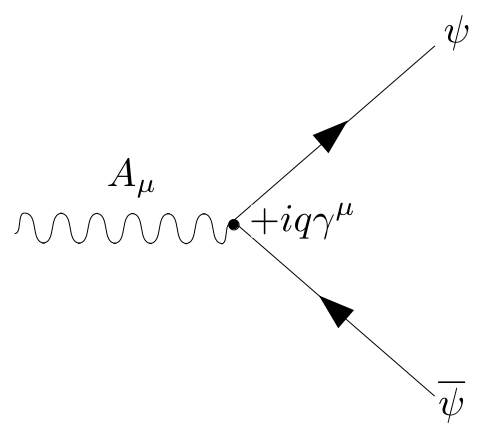
\includegraphics[scale=0.32]{Chapitre2/Images/psiApsi.png} 
            \caption{Vertex issu du terme de couplage du Lagrangien de la théorie électromagnétique quantique.}
        \label{psiApsi}
        \end{figure}

        En particulier, le troisième terme peut être interprété comme un couplage entre un courant de fermion $j^{\mu}=\overline{\psi}\gamma^{\mu}\psi$ tel qu'introduit dans la relation \ref{fermioncurrent} et le champ de jauge $A_{\mu}$. En terme de diagramme de Feynman, ce terme représente un point d'interaction appelé \textit{vertex} entre les champs avec une constante de couplage proportionnelle à la charge électrique $q$ (fig.\ref{psiApsi}). Pour une description complète du nouveau champ de jauge, il faut également ajouter au Lagrangien un terme cinématique et un terme de masse qui lui sont propres au même titre que pour les fermions. Le terme cinématique est directement issu du tenseur électromagnétique $F_{\mu\nu}$ avec pour expression 

        \begin{equation}
            F_{\mu\nu} = \partial_{\mu}A_{\nu}-\partial_{\nu}A_{\mu} 
                       =  \mqty(0 & E_x & E_y & E_z \\ 
                               -E_x & 0 & -B_z & B_y \\
                               -E_y & B_z & 0 & -B_x \\
                               -E_z & -B_y & B_x & 0)
        \end{equation}

        en convention quadrivectorielle $(+,-,-,-)$ et où $E$ et $B$ représentent les champs électrique et magnétique respectivement. \\
        
        Pour être correctement intégré dans le Lagrangien, $F_{\mu\nu}$ doit posséder une forme invariante de Lorentz dont la plus simple s'écrit $-\frac{1}{4}F_{\mu\nu}F^{\mu\nu}$. En revanche, l'ajout d'un terme de masse à la façon des solutions de l'équation de Klein-Gordon de la forme $\frac{1}{2}m^2A_{\mu}A^{\mu}$ brise l'invariance du Lagrangien est impose ainsi une masse nulle pour le photon. Finalement, le Lagrangien pour la QED s'écrit :

        \begin{equation}
            \boxed{\mathcal{L}_{\tiny QED} = \overline{\psi}\bigl(i\slashed{D}-m\bigr)\psi - \frac{1}{4}F_{\mu\nu}F^{\mu\nu},}
        \end{equation}

        avec $\slashed D = \gamma^{\mu}\bigl(\partial_{\mu}+iqA_{\mu}\bigr).$

        \subsection{Interaction faible}
        \label{weakinter}

        L'interaction faible intervient notamment à l'échelle atomique dans des mécanismes de désintégration nucléaire permettant à certains noyaux lourds de retrouver leur stabilité. Historiquement, elle a été introduite en 1930 par Enrico Fermi à travers une interaction à quatre fermions permettant d'expliquer la désintégration $\beta$ du neutron, et plus tard la désintégration du muon en électron observée en 1947. À l'échelle élémentaire, l'interaction faible agit sur les fermions et opère des changements de saveur de ces derniers à travers des courants chargés conduits par les bosons vecteurs $W^{\pm}$. Le couplage entre les bosons $W$ et les fermions possède également la particularité de ne pas conserver la parité. Cette transformation peut être formalisée par un opérateur $\hat{P}$ agissant sur une fonction d'onde en inversant ses coordonnées spatiales : 

        $$\psi(\vb{x},t)\rightarrow\psi'(\vb{x},t)=\hat{P}\psi(\vb{x},t)=\psi(-\vb{x},t).$$

        \begin{figure}
        \centering
            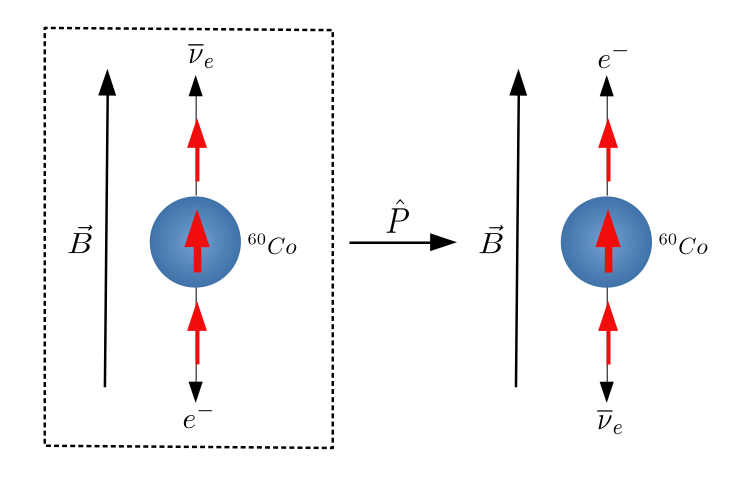
\includegraphics[scale=0.4]{Chapitre2/Images/wuexp.png} 
            \caption{Désintégration $\beta$ du $^{60}Co$. Sous l'action de la parité seules les directions d'émission de l'électron et de l'anti-neutrino sont inversées et la direction du spin est conservée. Seul le processus encadré faisant intervenir un anti-neutrino droit est autorisé.}
        \label{wuexp}
        \end{figure}

        En 1956, Chien-Shung Wu et ses collègues ont mis au point une expérience à travers laquelle des noyaux de cobalt 60 sont placés dans un champ magnétique dans le but d'aligner leurs moments magnétiques à la direction du champ \cite{Wu}. Dans le référentiel au repos du cobalt, un anti-neutrino et un électron sont émis dans des directions opposées au moment de sa désintégration. Par conservation du spin, chaque fermion possède un spin aligné avec le moment magnétique initial du cobalt. Par transformation de parité, seules les directions des particules émises sont affectées et la direction de leur spin est conservée. La figure \ref{wuexp} illustre les deux scénarios alors possibles. 

        \begin{enumerate}
            \item L'électron est émis dans la direction opposée au champ magnétique avec une impulsion anti-alignée à son spin tandis que l'anti-neutrino est émis dans la direction du champ avec une impulsion alignée à son spin.
            \item L'électron est émis dans la direction du champ magnétique avec une impulsion alignée à son spin tandis que l'anti-neutrino est émis dans la direction opposée au champ avec une impulsion anti-alignée à son spin.
        \end{enumerate}

        Si la parité est conservée, ces deux scénarios se réalisent avec autant de probabilité. Les physiciens ont observé une inhomogénéité dans la direction d'émission des électrons issus de la désintégration $\beta$, avec la direction opposée à celle du champ magnétique fortement favorisée, montrant ainsi que la parité n'est pas conservée par l'interaction faible. \\
        
        L'expérience permet également de montrer qu'à l'inverse l'interaction électromagnétique conserve la parité puisque les photons issus de la désexcitation du noyau de nickel après la désintégration du cobalt sont émis de manière homogène dans l'espace autour du noyau. Ce résultat se reflète dans la structure vectorielle du courant de fermion de l'interaction électromagnétique $j^{\mu}=\overline{\psi}\gamma^{\mu}\psi$, invariant sous la transformation de parité. Le courant faible est quant à lui composé à la fois d'un courant vectoriel et d'un courant pseudo-vectoriel de la forme $\overline{\psi}\gamma^{\mu}\gamma^5\psi$, avec $\gamma^5=i\gamma^0\gamma^1\gamma^2\gamma^3$, dont la combinaison est à l'origine de la violation de parité. L'expérience montre que cette combinaison possède une structure $V-A$ où $V$ est la partie vectorielle et $A$ la partie pseudo-vectorielle donnant lieu à l'expression du couplage faible :

        \begin{equation}
            \boxed{
            \frac{-ig_W}{2\sqrt{2}}\gamma^{\mu}\bigl(1-\gamma^5\bigr),
            }
        \end{equation}

        où $g_W$ est la constante de couplage de l'interaction faible intervenant aux vertex entre fermions et bosons $W^{\pm}$ tels que représentés dans les diagrammes de Feynman de la figure \ref{wdecay}. C'est par ailleurs la petite valeur de cette constante devant celle des autres interactions qui vaut à l'interaction faible son nom.\\
        
        Un autre concept qu'il convient de discuter dans la présentation de l'interaction faible est celui de la chiralité des particules élémentaires. Bien que sans équivalent classique, la chiralité est en réalité la limite ultra relativiste d'une grandeur appelée hélicité représentée par la projection du spin d'une particule sur son impulsion. Une particule dont le spin est aligné à l'impulsion sera dite d'hélicité droite tandis qu'elle sera d'hélicité gauche dans le cas inverse. A travers sa structure, l'interaction faible est capable de se coupler aux particules gauches et aux anti-particules droites uniquement. Mais contrairement à la chiralité, l'hélicité n'étant pas invariante de Lorentz, une particule peut toujours posséder une composante d'hélicité gauche indépendamment de sa chiralité et ainsi se coupler au courant faible, à l'exception du neutrino dont chiralité et hélicité sont toujours confondues en raison de son absence de masse. Il semble toutefois que seul le neutrino gauche et l'anti-neutrino droit soient présents dans la nature, illustrant la non conservation de la parité et la défavorisation du second scénario dans l'expérience de Wu. \\
        
        \begin{figure}
        \centering
            \includegraphics[scale=0.35]{Chapitre2/Images/wdecay.png} 
            \caption{Diagrammes de Feynman associés à la désintégration du muon (gauche) et à la désintégration $\beta^{+}$ (droite).}
        \label{wdecay}
        \end{figure}

        Historiquement, il a également été remarqué que la section efficace de production du processus de diffusion e$^+$e$^-\rightarrow W^+W^-$, reliée à sa probabilité d'occurrence, présente une divergence si seuls les diagrammes impliquant les particules connues à cette époque sont considérées. Cette divergence peut toutefois être corrigée par l'introduction d'un nouveau courant neutre conduit par le boson $Z^0$ tel que présenté dans les diagrammes de la figure \ref{eescat}. Le courant neutre sera finalement observé pour la première fois par l'expérience Gargamelle en 1973, dix ans avant la découverte du boson $Z^0$ en 1983. Son existence fut quant à elle prédite au cours des années 1960 dans le cadre de la théorie électrofaible, unifiant les interactions électromagnétique et faible et offrant un cadre théorique fondé sur la théorie quantique des champs. Une présentation de cette théorie sera donnée dans le paragraphe \ref{EWK} qui lui est consacré.

        \begin{figure}
        \centering
            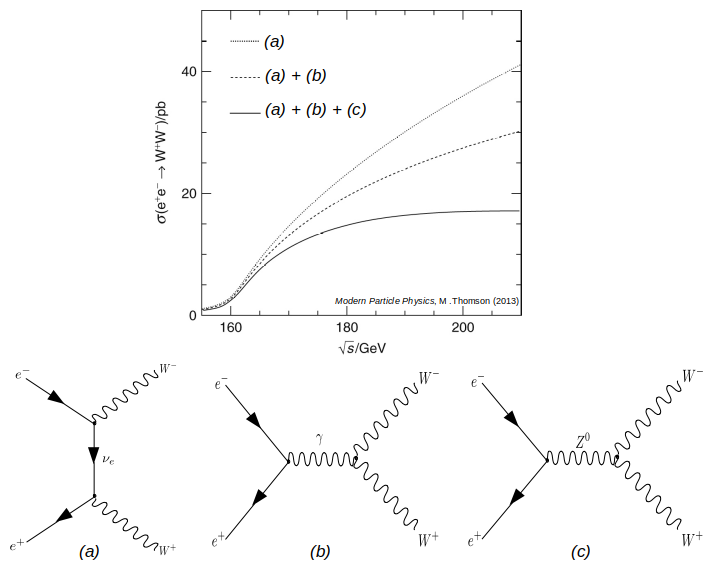
\includegraphics[scale=0.45]{Chapitre2/Images/eescatt.png} 
            \caption{Section efficace de production du processus e$^+$e$^-\rightarrow W^+W^-$ en fonction de l'énergie dans le centre de masse de la paire e$^+$e$^-$. La section efficace diverge si le courant neutre n'est pas considéré.}
        \label{eescat}
        \end{figure}
    
        \subsection{Interaction forte}
        \label{QCD}
        
        L'interaction forte permet à l'échelle atomique d'assurer la cohésion des noyaux grâce à une action attractive qui permet de contenir les effets répulsifs des interactions coulombiennes entre protons. A l'échelle élémentaire, elle permet aux quarks d'interagir pour former des hadrons à l'image du proton. Il s'agit aussi de la seule force dont l'énergie potentielle d'interaction est assimilable à celle d'un ressort avec une liberté asymptotique et résultant dans le confinement des quarks ne pouvant alors exister à l'état libre. La théorie quantique des champs décrivant l'interaction forte se nomme QCD (\textit{quantum chromodynamics}) et décrit son action sur les particules dotées d'une charge dites de \textit{couleur}, dont seuls les quarks sont dotés, à travers l'échange de gluons. \\

        Le Lagrangien de la QCD noté $\mathcal{L}_{\tiny QCD}$ peut être construit sur des principes similaires à ceux utilisés pour construire le Lagrangien de la QED en appliquant cette fois une transformation locale du groupe de symétrie SU($3$) telle que 

        \begin{equation}
            \psi\rightarrow\psi'=\exp[ig_S\vb*{\alpha}(\vb{x},t)\cdot\hat{\vb{T}}]\psi,
        \end{equation}

        où $\hat{\vb{T}}=\{T^a\}$ représente les huit générateurs de SU($3$) construits à partir des huit matrices de Gell-Mann données dans l'encadré \ref{gellmann} selon la relation

        $$T^a=\frac{1}{2}\lambda^a.$$

        \begin{figure}
        \begin{equation*}
        \boxed{
            \begin{array}{cc}
                    \lambda_1=\mqty(0&&1&&0 \\ 1&&0&&0 \\ 0&&0&&0), \quad
                    \lambda_2=\mqty(0&&-i&&0 \\ i&&0&&0 \\ 0&&0&&0), \quad
                    \lambda_3=\mqty(1&&0&&0 \\ 0&&-1&&0 \\ 0&&0&&0), \quad 
                    \vspace{8pt} \\
                    \lambda_4=\mqty(0&&0&&1 \\ 0&&0&&0 \\ 1&&0&&0), \quad
                    \lambda_5=\mqty(0&&0&&-i \\ 0&&0&&0 \\ i&&0&&0), \quad
                    \lambda_6=\mqty(0&&0&&0 \\ 0&&0&&1 \\ 0&&1&&0), \quad 
                    \vspace{8pt} \\
                    \lambda_7=\mqty(0&&0&&0 \\ 0&&0&&-i \\ 0&&i&&0), \quad
                    \lambda_8=\frac{1}{\sqrt{3}}\mqty(1&&0&&0 \\ 0&&1&&0 \\ 0&&0&&-2). \quad
            \end{array}
        }
        \end{equation*}
        \caption{Matrices de Gell-Mann.}
        \label{gellmann}
        \end{figure} 

        La dimension $3\times3$ des matrices de Gell-Mann impose à la fonction d'onde de contenir trois degrés de liberté associés à chacune des charges de couleur : rouge ($r$), verte ($g$) et bleue ($b$). Le maintient de l'invariance du Lagrangien de Dirac requiert alors l'introduction de huit nouveaux champs de jauge $G_{\mu}^{a=1\cdots8}$ associés aux gluons et se transformant selon

    \begin{equation}
        G_{\mu}^{a}\rightarrow G_{\mu}^{a'}=G_{\mu}^{a}-\partial_{\mu}\alpha_a-g_Sf_{abc}\alpha_aG_{\mu}^{b}.
    \label{glutrans}
    \end{equation}

    Le Lagrangien de Dirac devenu invariant sous une transformation locale du groupe SU($3$) s'écrit alors :

    \begin{equation}
        \mathcal{L}=\overline{\psi}\bigl(i\gamma^{\mu}(\partial_{\mu}+ig_SG_{\mu}^aT^a)-m\bigr)\psi.
    \end{equation}

    Ce Lagrangien contient, au même titre que la QED, un terme d'interaction entre les champs associés aux huit gluons et les fermions proportionnel à la constante de couplage de l'interaction forte $g_S$ et dérivé des courants de fermions. En revanche, les termes supplémentaires contenus dans la transformation des champs $G_{\mu}^a$ (éq. \ref{glutrans}) proviennent de la non commutation des matrices de Gell-Mann faisant de la QCD une théorie de jauge non abélienne et donnant naissance à des termes d'auto-interaction des gluons. Les diagrammes de Feynman issus des différents termes d'interaction du Lagrangien sont présentés dans la figure \ref{QCDdiag}. \\

    \begin{figure}
    \centering
        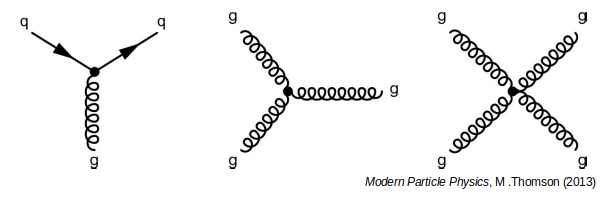
\includegraphics[scale=0.5]{Chapitre2/Images/QCDdiag.png} 
        \caption{Diagrammes de Feynman associés aux termes d'interaction et d'auto-interaction des gluons.}
    \label{QCDdiag}
    \end{figure}

    Finalement, la cinématique associée aux champs des gluons est contenue dans un tenseur de force $F^a_{\mu\nu}$ correspondant à la forme généralisée du tenseur électromagnétique pour une théorie non abélienne :

    \begin{equation}
        F^a_{\mu\nu}=\partial_{\mu}G^a_{\nu}-\partial_{\nu}G^a_{\mu}+g_Sf^{abc}A_{\mu}^bA_{\nu}^c
    \end{equation}

    dont la forme invariante de Lorentz la plus simple s'écrit $-\frac{1}{4}F^a_{\mu\nu}F^{a,\mu\nu}$. Le Lagrangien associé à la QCD prend alors la forme finale :

    \begin{equation}
    \boxed{
        \mathcal{L}_{\tiny QCD}=\overline{\psi}\bigl(i\slashed{D}-m\bigr)\psi - \frac{1}{4}F^a_{\mu\nu}F^{a,\mu\nu},
    }
    \end{equation}

    avec $\slashed D = \gamma^{\mu}\bigl(\partial_{\mu}+ig_SG^a_{\mu}T^a\bigr).$

    Par ailleurs, toute particule constituée de quarks doit posséder une charge de couleur totale neutre. Par cette contrainte, on distingue alors deux formes de hadrons : les mésons constitués d'une paire quark/anti-quark portant chacun respectivement une charge de couleur et une charge d'anti-couleur ($r\overline{r}$, $g\overline{g}$, $b\overline{b}$), et les baryons constitués de trois (anti-)quarks portant chacun une charge de (anti-)couleur ($rgb, \overline{r}\overline{g}\overline{b}$). Les échanges permanents de gluons entre les quarks de valence des hadrons donnent lieu à la formation d'une mer de quarks et de gluons virtuels appelés partons. Cette caractéristique est fondamentale dans le concept de collision de hadrons, puisqu'à haute énergie, cette mer devient "visible" pour une particule incidente. Ce concept découle directement de la relation de Louis de Broglie énoncée dans l'équation \ref{deBroglie}, indiquant que plus l'énergie d'une particule est élevée plus elle peut sonder profondément la matière.
    
    \section{Brisure de symétrie et unification électrofaible}
    \label{EWK}

    Un des buts fondamentaux des physiciens est de fournir une description unifiée des forces fondamentales de l'Univers. Au cours des années 1960, Sheldon Glashow, Abdus Salam et Steven Weinberg sont parvenus à fournir une description théorique unifiée de l'interaction électromagnétique et de l'interaction faible à travers un modèle dans lequel les deux interactions apparaissent comme deux aspects d'une seule, nommée interaction électrofaible. Au premier abord ces deux interactions semblent toutefois fondamentalement différentes avec d'une part un photon non massif de portée infinie et d'autre part trois bosons massifs de portée comparativement infiniment courte. Un éclairage peut être donné en analysant le groupe de symétrie associé à l'interaction faible. Par analogie à la transformation locale du groupe U($1$) \ref{localU1} introduite pour l'électromagnétisme, l'interaction faible émerge d'une transformation locale du groupe de symétrie SU($2$) :

    \begin{equation}
        \varphi\rightarrow\varphi'=\exp[ig_{W}\vb*{\alpha}(\vb{x},t)\cdot\vb{T}]\varphi,
    \label{localSU2}
    \end{equation}

    où $\vb{T}=\frac{1}{2}\vb*{\sigma}$ représente les trois générateurs du groupe SU($2$) constitués des matrices de Pauli $\sigma$. Cette transformation implique alors cette fois l'existence de trois bosons de jauge associés aux champs $W^{(1)}$, $W^{(2)}$ et $W^{(3)}$ pour satisfaire l'invariance du Lagrangien. De plus, la forme des matrices de Pauli impose à la fonction d'onde $\varphi$ de constituer un doublet dans lequel sont placés les deux fermions entre lesquels les courants chargés opèrent un changement de saveur en attribuant à chacun une charge d'isospin faible $I_W^{(3)}=\pm\sfrac{1}{2}$ pour une charge d'isospin faible totale du doublet $I_W=\sfrac{1}{2}$. En revanche, ces courants chargés ne pouvant affecter uniquement les particules gauches ces dernières sont placées dans des doublets dits gauches et notés $\varphi_L$ du groupe de symétrie SU($2$)$_L$, tandis que les particules droites sont placées individuellement dans des singlets de charge d'isospin faible nulle qui ne sont pas affectés par la transformation. La présence des champs de jauge $W_\mu^{k=1,2,3}$ résulte dans l'apparition d'un terme d'interaction entre ces champs et les fermions donnant naissance à trois courants

    \begin{equation*}
        j_1^{\mu}=\frac{g_W}{2}\overline{\varphi}_L\gamma^{\mu}\sigma_1\varphi_L, \quad
        j_2^{\mu}=\frac{g_W}{2}\overline{\varphi}_L\gamma^{\mu}\sigma_2\varphi_L, \quad
        j_3^{\mu}=\frac{g_W}{2}\overline{\varphi}_L\gamma^{\mu}\sigma_3\varphi_L,
    \end{equation*}

    à partir desquels peuvent être construits les courants associés à l'échange d'un boson $W^{\pm}$ :

    \begin{equation}
    \boxed{
        j^{\mu}_{\pm}=\frac{1}{\sqrt{2}}\bigl(j_1^\mu\pm ij^\mu_2\bigr)=\frac{g_W}{\sqrt{2}}\overline{\varphi}_L\gamma^\mu \sigma_{\pm}\varphi_L.
    }
    \label{Wexchange}
    \end{equation}

    Dans le cas du doublet constitué du neutrino électronique et de l'électron 

    \begin{equation*}
        \varphi_L=\mqty(\nu_{\mbox{\footnotesize e}} \\ \mbox{e}^-)_L,
    \end{equation*}

    les courants $j^{\mu}_{\pm}$ prennent la forme suivante :

    \begin{equation*}
    \begin{array}{ll}
        j^\mu_+ = \frac{g_W}{\sqrt{2}}\overline{\varphi}_L\gamma^{\mu}\sigma_+\varphi_L & = \frac{g_W}{\sqrt{2}}\mqty(\overline{\nu}_L&&\overline{\mbox{e}}_L)\gamma^\mu\mqty(0&&1\\0&&0)\mqty(\nu_L\\\mbox{e}_L) \\
        & = \frac{g_W}{\sqrt{2}}\overline{\nu}_L\gamma^{\mu}\mbox{e}_L, \\
        j^\mu_- = \frac{g_W}{\sqrt{2}}\overline{\varphi}_L\gamma^{\mu}\sigma_-\varphi_L & = \frac{g_W}{\sqrt{2}}\mqty(\overline{\nu}_L&&\overline{\mbox{e}}_L)\gamma^\mu\mqty(0&&0\\1&&0)\mqty(\nu_L\\\mbox{e}_L) \\
        & = \frac{g_W}{\sqrt{2}}\overline{\mbox{e}}_L\gamma^{\mu}\nu_L. \\
    \end{array}
    \end{equation*}

    Grâce à la définition des opérateurs de projection chirale gauche $\hat{P}_L$ et droit $\hat{P}_R$ 
    
    $$\hat{P}_L=\frac{1}{2}\bigl(1-\gamma^5\bigr), \quad \hat{P}_R=\frac{1}{2}\bigl(1+\gamma^5\bigr),$$
    
    les courants associés à l'échange d'un boson $W^{\pm}$ prennent alors la forme déjà décrite dans le paragraphe \ref{weakinter} dédié à l'interaction faible et illustrent les processus présentés dans les diagrammes de Feynman \ref{wdecay} :

    \begin{equation*}
    \boxed{
        j^\mu_+ = \frac{g_W}{2}\overline{\nu}\gamma^{\mu}\frac{1}{2}\bigl(1-\gamma^5\bigr)\mbox{e} \quad \mbox{ et } \quad j^\mu_- = \frac{g_W}{2}\overline{\mbox{e}}\gamma^{\mu}\frac{1}{2}\bigl(1-\gamma^5\bigr)\nu.
    }
    \end{equation*}

    Le dernier courant $j^\mu_3$ prend quant à lui la forme d'un courant neutre au sein d'un doublet de fermions sans opérer de changement de saveur :

    $$\boxed{j^\mu_3=I^{(3)}_Wg_W\overline{\varphi}\gamma^\mu\frac{1}{2}\bigl(1-\gamma^5\bigr)\varphi.}$$

    Les singlets droits ne possédant pas de charge d'isospin faible, le courant neutre $j^\mu_3$ est capable de se coupler aux particules gauches uniquement. L'expérience montre en revanche que le boson $Z^0$ est capable de se coupler indépendamment aux particules gauches et droites le rendant incompatible avec le boson de jauge $W^{(3)}$. En se basant sur la neutralité du photon dans le cadre de la QED, les physiciens ont alors supposé l'existence d'un nouveau boson neutre issu d'un champ vectoriel $B^\mu$ émergeant d'une transformation de jauge locale du groupe de symétrie U($1$)$_Y$ telle que :

    \begin{equation}
        \psi\rightarrow\psi'=\exp[ig'\frac{\mbox{Y}}{2}\zeta(\vb{x},t)]\psi,
    \label{localU1Y}
    \end{equation}

    où la charge conservée associée est l'hypercharge Y. Les champs $A_\mu$ et $Z_\mu$ peuvent alors être exprimés comme une combinaison linéaire des champs de jauge $B_\mu$ et $W^{(3)}_\mu$ :

    \begin{equation}
    \begin{array}{ll}
         A_\mu & = +B_\mu\cos\theta_W+W^{(3)}_\mu\sin\theta_W \\
         Z_\mu & = -B_\mu\sin\theta_W+W^{(3)}_\mu\cos\theta_W
    \end{array}
    \end{equation}

    où $\theta_W$, appelé \textit{angle de Weinberg}, représente l'angle de mélange électrofaible défini à partir des constantes de couplage de l'interaction électromagnétique et de l'interaction faible :

    $$\sin^2\theta_W=\frac{q^2}{g^2_W}\approx 0.23,$$

    et dont les valeurs mesurées expérimentalement sont à ce jour en accord avec la valeur prédite par le modèle standard. Dans le cas où cet angle est nul, les champs physiques associés au photon et au boson $Z^\mu$ coïncident alors avec les champs de jauges issus de SU($2$)$_L\times$U($1$)$_Y$. Ce paramètre représente le degré de brisure de symétrie du groupe SU($2$)$_L$ et de mélange avec le groupe U($1$)$_Y$, donnant au boson $Z^0$ la particularité de se coupler différemment aux particules gauches et droites. Ce résultat est à l'origine de nombreux phénomènes physiques tels que la polarisation des fermions produits dans des états d'hélicité asymétriques. Ce modèle seul en revanche ne permet pas de décrire l'origine de cette brisure de symétrie ni celle de la masse des bosons de jauge de l'interaction faible. Ces aspects nécessitent en réalité l'existence d'un boson additionnel de nature scalaire intervenant à travers un mécanisme explicité dans le paragraphe \ref{higgsmeca}.

    \section{Le boson de Higgs}

        Suite au développement de la théorie électrofaible, plusieurs physiciens dont François Englert, Robert Brout et Peter Higgs ont prédit en 1964 l'existence d'un nouveau boson à l'origine de la brisure de symétrie électrofaible \cite{BE,H}. Né d'un champ scalaire, ce boson nommé par la suite boson de Higgs constitue alors la seule particule élémentaire au sein du modèle standard dont le spin est nul et dont la fonction d'onde est invariante sous une transformation CP. Bien que sa masse ne soit pas prédite par le modèle, des observations expérimentales compatibles avec ce type de particule ont attribué aux expériences ATLAS et CMS en 2012 la découverte du boson de Higgs avec une masse avoisinant 125 GeV. Cette partie sera dédiée dans un premier temps à l'introduction des brisures de symétrie spontanées, puis dans un second temps au mécanisme BEH durant lequel la brisure de symétrie électrofaible s'opère, résultant dans la génération de la masse des bosons $W^{\pm}$ et $Z^0$. Enfin les couplages de Yukawa, à travers lesquels les fermions se couplent au boson de Higgs et acquièrent une masse, seront présentés.

        \subsection{Brisure de symétrie spontanée}

        Telles qu'introduites dans la partie \ref{sectionQFT}, les particules scalaires sont issues de champs dont les équations du mouvement sont gouvernées par l'équation de Klein-Gordon \ref{KG}. Le Lagrangien dans le cas d'un champ scalaire $\phi$ libre et purement réel s'écrit

        \begin{equation}
            \mathcal{L}=\frac{1}{2}\bigl(\partial_{\mu}\phi\bigr)\bigl(\partial^{\mu}\phi\bigr).
        \label{lagscalaire}
        \end{equation}

        Tandis que ce Lagrangien contient uniquement la cinématique du champ, nous faisons le choix d'y ajouter un potentiel $V(\phi)$ constitué d'un terme de masse $\frac{1}{2}\mu^2\phi^2$ et d'un terme de la forme $\frac{1}{4}\lambda\phi^4$ représentant une auto-interaction à quatre points de $\phi$ avec une constante de couplage $\lambda$. Le Lagrangien \ref{lagscalaire} devient alors :

        \begin{equation}
        \begin{array}{ll}
            \mathcal{L}&=\frac{1}{2}\bigl(\partial_{\mu}\phi\bigr)\bigl(\partial^{\mu}\phi\bigr)-V(\phi) \vspace{4pt}\\
                       &=\frac{1}{2}\bigl(\partial_{\mu}\phi\bigr)\bigl(\partial^{\mu}\phi\bigr)-\frac{1}{2}\mu^2\phi^2-\frac{1}{4}\lambda\phi^4.
        \end{array}
        \label{laghiggs}
        \end{equation}

        Bien que $\lambda$ soit contraint à une valeur positive pour éviter la divergence de la valeur minimale de $V(\phi)$, $\mu^2$ peut quant à lui prendre une valeur aussi bien positive que négative. Dans le premier cas, le minimum du potentiel est atteint lorsque $\phi=0$ avec une valeur $V(\phi)=0$ (fig. \ref{HiggsV1D}), tandis que dans le second cas le minimum est atteint pour deux valeurs distinctes de $\phi$ constantes et non nulles :

        \begin{equation}
            \phi=\pm\nu=\pm\displaystyle\left\lvert \sqrt{\frac{-\mu^2}{\lambda}} \right\rvert.
        \end{equation}

        \begin{figure}
        \centering
            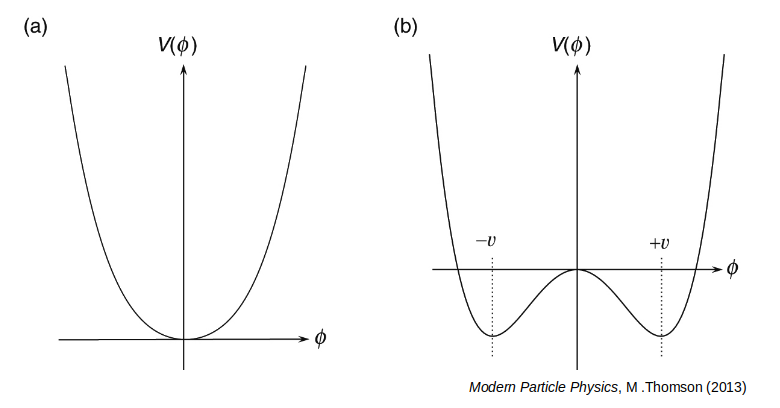
\includegraphics[scale=0.4]{Chapitre2/Images/higgsV1D.png} 
            \caption{Représentation graphique du potentiel $V(\phi)$ pour $\mu^2>0$ (a) et $\mu^2<0$ (b).}
        \label{HiggsV1D}
        \end{figure}

        La valeur non nulle du champ à son minimum de potentiel constitue sa valeur moyenne dans le vide (v.e.v, \textit{vacuum expectation value}), et c'est le choix arbitraire d'une de ses valeurs $\pm\nu$ qui constitue la \textit{brisure de symétrie spontanée} du Lagrangien \ref{laghiggs}. Dans la suite nous considérons une brisure de symétrie vers la valeur positive du champ $+\nu$ et nous introduirons une excitation $\eta(x)$ de ce dernier, assimilée à la création d'une particule, telle que $\phi(x)=\nu+\eta(x)$. Le Lagrangien du champ scalaire devient alors après développement

        \begin{equation*}
        \boxed{
            \mathcal{L}=\frac{1}{2}\bigl(\partial_{\eta}\phi\bigr)\bigl(\partial^{\mu}\eta\bigr)-\lambda\mu^2\eta^2-\lambda\nu\eta^3-\frac{1}{4}\lambda\eta^4+\frac{1}{4}\lambda\nu^4,
        }
        \end{equation*}

        et est constitué des termes suivants :

        \begin{enumerate}
            \item[$\bullet$] $\frac{1}{2}\bigl(\partial_{\eta}\phi\bigr)\bigl(\partial^{\mu}\eta\bigr)$ : terme cinématique associé à $\eta$,
            \item[$\bullet$] $\lambda\mu^2\eta^2$ : terme de masse associé à $\eta$ avec $m_{\eta}=\sqrt{-2\mu^2}$,
            \item[$\bullet$] $\lambda\nu\eta^3,\;\frac{1}{4}\lambda\eta^4$ : interactions à trois et quatre points (fig. \ref{higgsVtx}),
            \item[$\bullet$] $\frac{1}{4}\lambda\nu^4$ : constante sans implication physique.
        \end{enumerate}

        Ce nouveau Lagrangien constitue la représentation physique de l'excitation d'un champ scalaire massif autour de sa valeur moyenne dans le vide après une brisure de symétrie spontanée.

        \begin{figure}
        \centering
            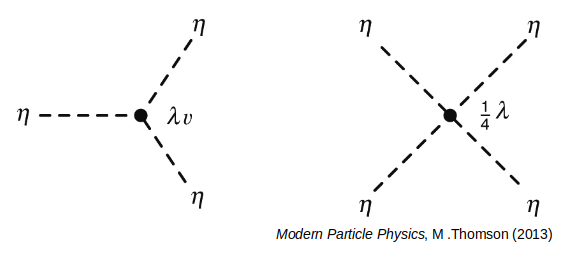
\includegraphics[scale=0.45]{Chapitre2/Images/higgsVtx.png} 
            \caption{Diagrammes de Feynman des auto-interactions du champ scalaire $\eta$ à trois et quatre points.}
        \label{higgsVtx}
        \end{figure}

        \subsection{Mécanisme de Brout-Englert-Higgs (BEH)}
        \label{higgsmeca}

        De façon générale, le mécanisme BEH constitue une démarche visant à introduire une brisure de symétrie spontanée pour un champ scalaire dans une théorie de jauge. Ce processus a pour résultat l'apparition d'un champ de jauge massif dont la nature dépend du groupe de symétrie initialement choisi pour la transformation du Lagrangien, et dont la masse est générée par des interactions avec le champ scalaire. Dans le cas du modèle électrofaible, la théorie de jauge choisie est celle associée au groupe de symétrie SU($2$)$_L\times$U($1$)$_Y$ introduit plus tôt dans le paragraphe \ref{EWK}. Afin d'être compatible avec le nombre de degrés de liberté nécessaire, $\phi$ doit être constitué de deux champs scalaires complexes placés dans un doublet d'isospin faible tel que 

        \begin{equation}
            \phi = \mqty(\phi^+ \\ \phi^0) = \frac{1}{\sqrt{2}}\mqty(\phi_1+i\phi_2 \\ \phi_3 + i\phi_4),
        \label{higgsdoublet}
        \end{equation}

        et dont le Lagrangien s'écrit 

        \begin{equation}
        \begin{array}{ll}
            \mathcal{L}&=\bigl(\partial_{\mu}\phi\bigr)^{\dag}(\partial^{\mu}\phi\bigr)-V(\phi) \vspace{5pt} \\
            &=\bigl(\partial_{\mu}\phi\bigr)^{\dag}(\partial^{\mu}\phi\bigr)-\mu^2\phi^{\dag}\phi-\lambda\bigl(\phi^{\dag}\phi\bigr)^2,
        \end{array}
        \label{HiggsLag}
        \end{equation}

        \begin{figure}
        \centering
            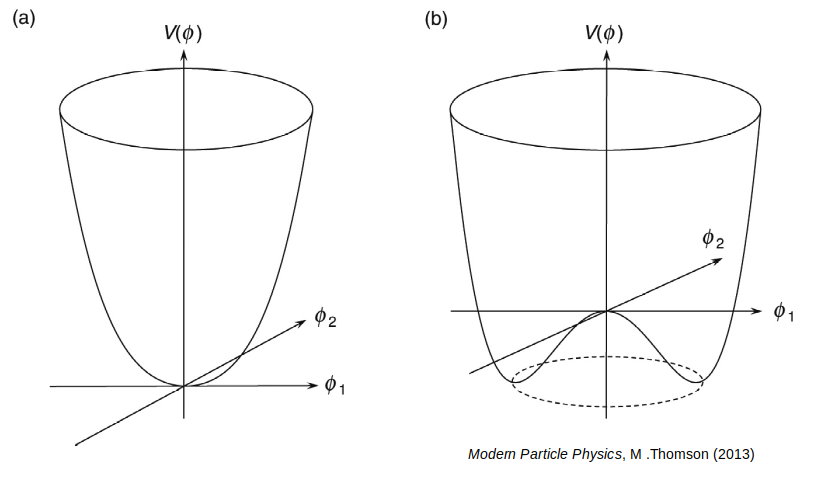
\includegraphics[scale=0.4]{Chapitre2/Images/higgsV3D.png} 
            \caption{Représentation graphique du potentiel de Higgs pour $\mu^2>0$ (a) et $\mu^2<0$ (b).}
        \label{HiggsV3D}
        \end{figure}

        où $V(\phi)$ constitue le potentiel de Higgs avec des paramètres similaires à ceux introduits dans le Lagrangien \ref{laghiggs}. Pour un champ complexe $\phi_1+i\phi_2$, le potentiel présente cette fois une dégénérescence infinie de minima (fig. \ref{HiggsV3D}) pour $\mu^2<0$ sur un cercle satisfaisant l'équation $$\phi_1^2+\phi_2^2=\frac{-\mu^2}{\lambda}=\nu^2.$$ En revanche seul un champ scalaire neutre peut posséder une valeur moyenne dans le vide non nulle afin de conserver la charge électrique et ainsi la v.e.v du doublet d'isospin faible $\phi$ s'écrira $$\ev{\phi}{0}=\frac{1}{\sqrt{2}}\mqty(0 \\ \nu).$$ Après excitation du champ autour de cette dernière, $\phi$ prend alors la forme

        \begin{equation}
            \phi(x)=\frac{1}{\sqrt{2}}\mqty(\phi_1(x)+i\phi_2(x) \\ \nu+\eta(x)+i\phi_4(x)).
        \end{equation}
        
        L'invariance de \ref{HiggsLag} sous une transformation de SU($2$)$_L\times$U($1$)$_Y$ peut quant à elle être conservée en introduisant la dérivée covariante suivante :

        \begin{equation}
            \partial_{\mu}\rightarrow D_{\mu}=\partial_{\mu}+ig_W\vb{T}\cdot\vb{W}_{\mu}+ig'\frac{\mbox{Y}}{2}B_{\mu},
        \label{higgsdcov}
        \end{equation}

        dont les termes sont ceux issus des transformations locales \ref{localSU2} et \ref{localU1Y}. De manière générale, l'ajout d'une dérivée covariante au sein du Lagrangien produit un terme de masse pour les champs de jauge mais également de nouveaux champs reliés à des bosons scalaires sans masse appelés bosons de Goldstone. Ces derniers peuvent se coupler aux champs de jauge grâce à des termes d'interaction à travers lesquels un boson de jauge vectoriel devient scalaire, et n'ont donc pas de réalité physique. Il est toutefois possible de les éliminer avec l'ajout d'une nouvelle jauge, on dit alors que les bosons de Goldstone sont "mangés" par les champs de jauge. Ce mécanisme entraîne l'apparition d'un nouveau degré de polarisation longitudinal des bosons de jauge correspondant au troisième degré de projection du spin $S_z=0$ propre aux particules massives de spin $1$. En réalité la démarche visant à éliminer les bosons de Goldstone peut être contournée en évitant leur apparition avec le même résultat final en choisissant initialement une jauge dite unitaire pour le champ scalaire telle que seul le champ d'excitation persiste et soit purement réel. Dans le cas du mécanisme BEH électrofaible on obtient alors :

        \begin{equation}
            \phi=\frac{1}{\sqrt{2}}\mqty(0 \\ \nu+h(x)),
        \label{higgsunit}
        \end{equation}

        où $h(x)$ désigne cette fois le \textit{champ de Higgs}. La masse des bosons de jauge peut être déterminée à partir du terme cinétique du Lagrangien $\bigl(D_{\mu}\phi\bigr)^{\dag}\bigl(D^{\mu}\phi\bigr)$ dans lequel ont été introduits la dérivée covariante \ref{higgsdcov} et la jauge unitaire \ref{higgsunit} :

        \begin{equation*}
        \begin{array}{ll}
            \bigl(D_{\mu}\phi\bigr)^{\dag}\bigl(D^{\mu}\phi\bigr) = & \frac{1}{2}\bigl(\partial_{\mu}h\bigr)\bigl(\partial^{\mu}h\bigr) \vspace{5pt} \\
            & +\frac{1}{8}g_W^2\bigl(W^{(1)}_{\mu}+iW^{(2)}_{\mu}\bigr)\bigl(W^{(1),\mu}-iW^{(2),\mu}\bigr)(\nu+h)^2 \vspace{5pt} \\
            & +\frac{1}{8}\bigl(g_WW^{(3)}_{\mu}-g'B_{\mu}\bigr)\bigl(g_WW^{(3),\mu}-g'B^{\mu}\bigr)(\nu+h)^2.
        \end{array}
        \end{equation*}

        On reconnaît en particulier dans le second terme de ce résultat la double combinaison des champs $W^{(1)}$ et $W^{(2)}$ dont la structure est semblable à celle des courants chargés \ref{Wexchange} associés à l'échange des bosons $W^{\pm}$. Afin de déterminer les termes de masse, il convient de développer les termes quadratiques dans lesquels interviennent les champs de jauge. De cette façon nous obtenons pour les bosons $W^{\pm}$ :

        \begin{equation*}
        \begin{array}{ll}
            \frac{1}{8}\nu^2g^2_W\bigl(W^{(1)}_{\mu}W^{(1),\mu}&+W^{(2)}_{\mu}W^{(2),\mu}\bigr) \vspace{5pt}\\
            &=\frac{1}{2}m^2_W\bigl(W^{(1)}_{\mu}W^{(1),\mu}+W^{(2)}_{\mu}W^{(2),\mu}\bigr),
        \end{array}
        \end{equation*}

        avec

        \begin{equation}
            \boxed{
            m_W=\frac{1}{2}g_W\nu.
            }
        \end{equation}

        Le terme associé aux champs $W_{\mu}^{(3)}$ et $B_{\mu}$ peut quant à lui s'écrire sous la forme matricielle suivante :

        \begin{equation*}
        \begin{array}{ll}
            \frac{\nu^2}{8}\mqty(W^{(3)}_{\mu}&&B_{\mu})&\mqty(g^2_W&&-g_Wg'\\-g_Wg'&&g'^2)\mqty(W^{(3),\mu}\\B^{\mu}) \vspace{5pt} \\
            &=\frac{\nu^2}{8}\mqty(W^{(3)}_{\mu}&&B_{\mu})\vb{M}\mqty(W^{(3),\mu}\\B^{\mu}),
        \end{array}
        \end{equation*}

        où $\vb{M}$ représente une matrice non-diagonale de masse à travers laquelle les champs $W_{\mu}^{(3)}$ et $B_{\mu}$ se mélangent. En opérant un changement de base dans laquelle cette matrice est diagonale, il est alors possible de définir la structure des champs correspondant à des bosons physiques dont les masses seront données par les termes diagonaux $\lambda$ de $\vb{M}$ obéissant à l'équation $\det(\vb{M}-\lambda I)=0$. Dans le cas de l'interaction électrofaible, les bosons physiques recherchés correspondent au photon et au boson $Z^0$, respectivement associés aux champs $A_{\mu}$ et $Z_{\mu}$ introduits plus tôt. Dans la nouvelle base on obtient alors :

        \begin{equation*}
        \begin{array}{ll}
            \frac{\nu^2}{8}\mqty(A_{\mu}&&Z_{\mu})&\mqty(0&&0\\0&&g^2_W+g'^2)\mqty(A^{\mu}\\Z^{\mu}) \vspace{5pt} \\
            &=\frac{1}{2}\mqty(A_{\mu}&&Z_{\mu})\mqty(m_A^2&&0\\0&&m_Z^2)\mqty(A^{\mu}\\Z^{\mu}),
        \end{array}
        \end{equation*}    

        et ainsi 

        \begin{equation}
            \boxed{
            m_A=0 \quad \mbox{et} \quad m_Z=\frac{1}{2}\nu\sqrt{g^2_W+g'^2}.
            }
        \end{equation}

        Il est alors intéressant de noter que tandis que le photon reste sans masse après brisure de symétrie, les bosons de l'interaction faible ont acquis une masse dont la valeur est proportionnelle à la valeur moyenne dans le vide du champ de Higgs. Le Lagrangien contient également désormais des termes d'interaction dont la structure permet de définir les diagrammes de Feynman présents dans la figure \ref{higgsVcoupling}

        \begin{figure}
        \centering
            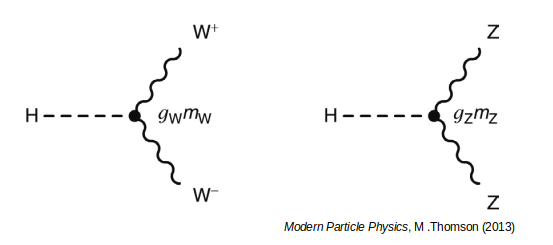
\includegraphics[scale=0.45]{Chapitre2/Images/higgsVcoupling.png} 
            \caption{Diagrammes de Feynman des couplages entre le boson de Higgs $H$ et les bosons $W^{\pm}$ et $Z^0$.}
        \label{higgsVcoupling}
        \end{figure}
        
        \subsection{Couplages de Yukawa}
        \label{yukawa}

        Le mécanisme BEH introduit dans la partie précédente permet de déterminer l'origine de la masse des bosons de l'interaction faible et de leur degré supplémentaire de polarisation longitudinale tout en conservant l'absence de masse du photon. En revanche l'origine de la masse des fermions reste inexpliquée à ce stade. Le terme de masse associé aux fermions dans le Lagrangien de Dirac peut être exprimé en fonction des composantes chirales gauche et droite des spineurs de Dirac $\psi$ de façon à obtenir $$-m\overline{\psi}\psi=m\bigl(\overline{\psi}_R\psi_L+\overline{\psi}_L\psi_R\bigr).$$ Ce terme n'est cependant pas invariant sous une transformation du groupe de symétrie SU($2$)$_L\times$U($1$)$_Y$. De la même façon que lors de l'introduction de l'unification électrofaible dans la partie \ref{EWK}, les fermions de chiralité gauche $\psi_L$ sont placés dans des doublets de SU($2$), tandis que les fermions de chiralité droite $\psi_R$ sont placés dans des singlets. Puisque les champs complexes \ref{higgsdoublet} du mécanisme BEH sont eux aussi placés dans un doublet $\phi$, la combinaison $\overline{\psi}_L\phi$ de ce dernier avec $\psi_L$ est elle aussi invariante sous une transformation de SU($2$). Il est alors possible de définir une forme de couplage invariante sous une transformation de SU($2$)$_L\times$U($1$)$_Y$ à partir d'une combinaison du terme précédent avec un singlet $\psi_R$ et une constante de couplage propre à chaque fermion s'écrivant $-g_f\bigl(\overline{\psi}_L\phi\psi_R+\overline{\psi}_R\phi^{\dag}\psi_L\bigr)$. En choisissant un exemple à partir du doublet et du singlet contenant l'électron et en appliquant à $\phi$ la jauge unitaire \ref{higgsunit}, le Lagrangien associé peut s'écrire sous la forme

        \begin{align*}
             \mathcal{L}_e & = -\frac{g_e}{\sqrt{2}}\mqty[\mqty(\overline{\nu}_e&&\overline{e})_L\mqty(0\\\nu+h(x))e_R+\overline{e}_R\mqty(0&&\nu+h(x))\mqty(\nu_e\\e)_L] \vspace{5pt} \\
             & = -\frac{g_e}{\sqrt{2}}\nu\bigl(\overline{e}_Le_R+\overline{e}_Re_L\bigr)-\frac{g_e}{\sqrt{2}}h\bigl(\overline{e}_Le_R+\overline{e}_Re_L\bigr) \vspace{5pt} \\
             & = -\frac{g_e}{\sqrt{2}}\bigl(\nu\overline{e}e+h\overline{e}e\bigr).
        \end{align*}

        La valeur de la constante de couplage présente dans le Lagrangien n'étant pas prédite par le mécanisme BEH, elle est librement choisie comme étant reliée à la masse $m_e$ de l'électron et telle que $$g_e=\sqrt{2}\frac{m_e}{\nu}.$$ Le Lagrangien peut alors être étendu à tous les fermions avec la forme générale

        \begin{equation}
        \boxed{
            \mathcal{L}_f=-\frac{g_f}{\sqrt{2}}\bigl(\nu\overline{\psi}\psi+h\overline{\psi}\psi\bigr) \vspace{5pt}=-m_f\overline{\psi}\psi-\frac{m_f}{\nu}\overline{\psi}\psi h
        ,}
        \label{yukawacoupling}
        \end{equation}

        où $g_f$ représente les \textit{couplages de Yukawa} des fermions \cite{Yukawa}. Le second terme illustre le couplage entre le boson de Higgs et les fermions dont le diagramme de Feynman est donné dans la figure \ref{higgsfcoupling}.



        \begin{figure}
        \centering
            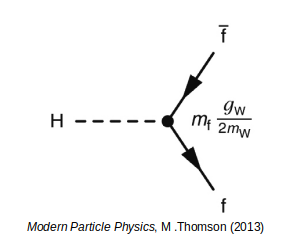
\includegraphics[scale=0.45]{Chapitre2/Images/higgsfcoupling.png} 
            \caption{Diagramme de Feynman du couplage entre le boson de Higgs $H$ et les fermions.}
        \label{higgsfcoupling}
        \end{figure}
        

    %\chapter{Le \textit{\uppercase{L}arge \uppercase{H}adron \uppercase{C}ollider} et le détecteur CMS}
\label{chap4}

La seconde guerre mondiale eut pour conséquence sur l'Europe une fuite des cerveaux vers les États-Unis entraînant la perte de son rayonnement international en matière de recherche en physique. Sur ce constat, plusieurs physiciens notables de l'époque parmi lesquels figurent Edoardo Amaldi, Pierre Auger et Niels Bohr émettent l'idée de la création d'un nouveau laboratoire de recherche en physique nucléaire a l'échelle européenne. Louis de Broglie fut le premier à proposer un tel projet lors de la conférence européenne de la culture à Lausanne en décembre 1949, dont le principal argument retenu sera celui du partage des coûts entre les nations, sans encore bénéficier du soutien des gouvernements. Cette proposition sera suivie d'une seconde en juin 1950 lors de la conférence générale de l'UNESCO à Florence, sous l'impulsion du physicien américain Isidor Rabi, prônant la nécessité d'une collaboration scientifique internationale. En 1951, un conseil provisoire baptisé Conseil Européen pour la Recherche Nucléaire est fondé menant à la ratification en 1954 de la première convention officielle du CERN par 12 nations européennes. Le choix de l'emplacement est porté vers la Suisse pour sa position centrale au sein de l'Europe et sa neutralité, avec la pose de la première pierre à l'édifice sur le site de Meyrin en juin 1955 par Felix Bloch alors directeur général du CERN. \\

Dès 1957 le CERN lance la construction de son premier accélérateur de particules. Il s'agira d'un synchrocyclotron (SC) permettant de conduire un faisceau de protons d'une énergie de $600$ MeV sur une cible fixe, menant à l'observation de la désintégration rare du pion en électron seulement quelques heures après son démarrage en 1958. En 1959, le CERN met en fonction son premier synchrotron à protons (PS, \textit{Proton Synchrotron}) atteignant une énergie de $28$ GeV et devenant pendant une brève période l'accélérateur le plus puissant du monde devançant de $10$ GeV le record  établi par l'URSS. \\

En 1968, l'invention de la chambre à fils par le physicien français Georges Charpak révolutionne le concept de détection en physique des particules. Le détecteur se compose d'une enceinte remplie de gaz inerte dans laquelle des grilles constituées de fils parallèles sous tension sont empilées par alternance de cathodes et d'anodes. Le passage d'une particule chargée entraîne ainsi l'ionisation du gaz et un déplacement de charges mesurable sous la forme d'une impulsion électrique. Cette technique rend désormais possible le traitement informatique des données et viendra rapidement remplacer les chambres à bulles pour lesquelles une analyse image par image "à la main" des traces produites était nécessaire. \\

Le début des années 70 marque le début des premières collisions proton-proton au sein de l'ISR (\textit{Intersecting Storage Ring}), un nouvel accélérateur alimenté par le PS. Avec une énergie dans le centre de masse de $62$ GeV, le concept de croisement de faisceaux permet un accès à des hautes énergie en produisant le même effet qu'une collision sur cible fixe à une énergie de $2000$ GeV. Durant 13 années d'opération, l'ISR aura notamment permis un sondage profond de la matière en offrant aux physiciens les premiers indices de la nature composite du proton. Il servira également d'instrument pour le développement du refroidissement stochastique inventé par Simon van der Meer, permettant d'augmenter et d'uniformiser significativement la densité d'énergie des faisceaux de particules chargées. En parallèle, le CERN lance son projet de construction du Super Proton Synchrotron (SPS), un collisionneur proton-proton sous-terrain de $7$ km de diamètre, lancé en 1976. Il sera par la suite converti en collisionneur proton-antiproton en 1979 suivant l'initiative de Carlo Rubia et Simon van der Meer menant à la découverte des bosons $W$ et $Z$ en 1983 par les expériences UA$1$ et UA$2$. \\

L'année 1988 est marquée par l'injection du premier faisceau dans le \textit{Large Electron-Positron} (LEP) \textit{collider}. Ce collisionneur d'un diamètre de $27$ km fut capable de produire des collisions électron-positron à une énergie dans le centre de masse de $100$ GeV à son lancement et jusqu'à $209$ GeV à la fin de son exploitation le 2 novembre 2000. Le LEP servit à réaliser de nombreuses mesures de précision confortant les prédictions apportées par le modèle standard dans le secteur électrofaible, et notamment en contraignant à trois le nombre de générations de fermions via la mesure de la largeur de désintégration du boson $Z$ \cite{ZALEPH,ZDELPHI,ZL3,ZOPAL}. Les travaux d'excavation réalisés pour la mise en place de l'accélérateur et de ses expériences servirent ensuite de base à la mise en place de l'actuel \textit{Large Hadron Collider} (LHC) et de ses quatre expériences majeures : CMS, ATLAS, ALICE et LHCb. \\

\section{LHC, \textit{\uppercase{L}arge \uppercase{H}adron \uppercase{C}ollider}}

Le 18 septembre 2008, le premier faisceau de protons est injecté avec succès au sein du LHC d'un diamètre de $27$ km et situé à une profondeur moyenne de $100$ m. Les physiciens se tiennent alors prêts à entrer dans une nouvelle ère de découvertes à des échelles d'énergie jamais atteintes. La machine promet un programme de physique large, allant de la recherche du boson de Higgs et de nouvelles particules s'inscrivant dans une physique \textit{au-delà du modèle standard}, à l'étude de l'évolution de la matière dans les premiers instants de l'Univers.

\subsection{Caractéristiques techniques}

L'injection des deux faisceaux dans le LHC circulant en sens opposés est assurée par un complexe d'accélérateurs constitué de ses prédécesseurs (Fig. \ref{complex}). Au départ, les protons sont issus de dihydrogène duquel les électrons sont arrachés par un champ électrique produit dans un cylindre métallique appelé duoplasmatron. Ils sont ensuite regroupés en paquets et accélérés à une énergie de $750$ keV avant d'être injectés dans un accélérateur linéaire, le LINAC$2$, pour atteindre une énergie de $50$ MeV. Depuis 2020, le LINAC$4$ succède au LINAC$2$ en fournissant un faisceau d'ions $H^-$ porté à une énergie de $160$ MeV. Les protons sont ensuite amenés respectivement à une énergie de $1,4$ GeV en sortie du booster, $26$ GeV en sortie du PS et atteignent finalement $450$ GeV en sortie du SPS au moment de l'injection dans le LHC et avant d'être à nouveau accélérés par $16$ cavités radiofréquence jusqu'à leur énergie nominale. Jusqu'à la fin de la seconde phase d'exploitation du LHC en 2018 (Run 2), chaque faisceau pouvait emporter jusqu'à 2556 paquets de protons eux-mêmes constitués d'une centaine de milliards de protons. Ces chiffres ont été revus à la hausse pour la troisième phase d'exploitation (Run 3) démarrée en 2022 et encore en cours à ce jour en 2023, permettant d'augmenter la quantité de collisions produites aussi appelée \textit{luminosité instantanée}. Celle-ci est définie par : 

\begin{figure}
\centering
    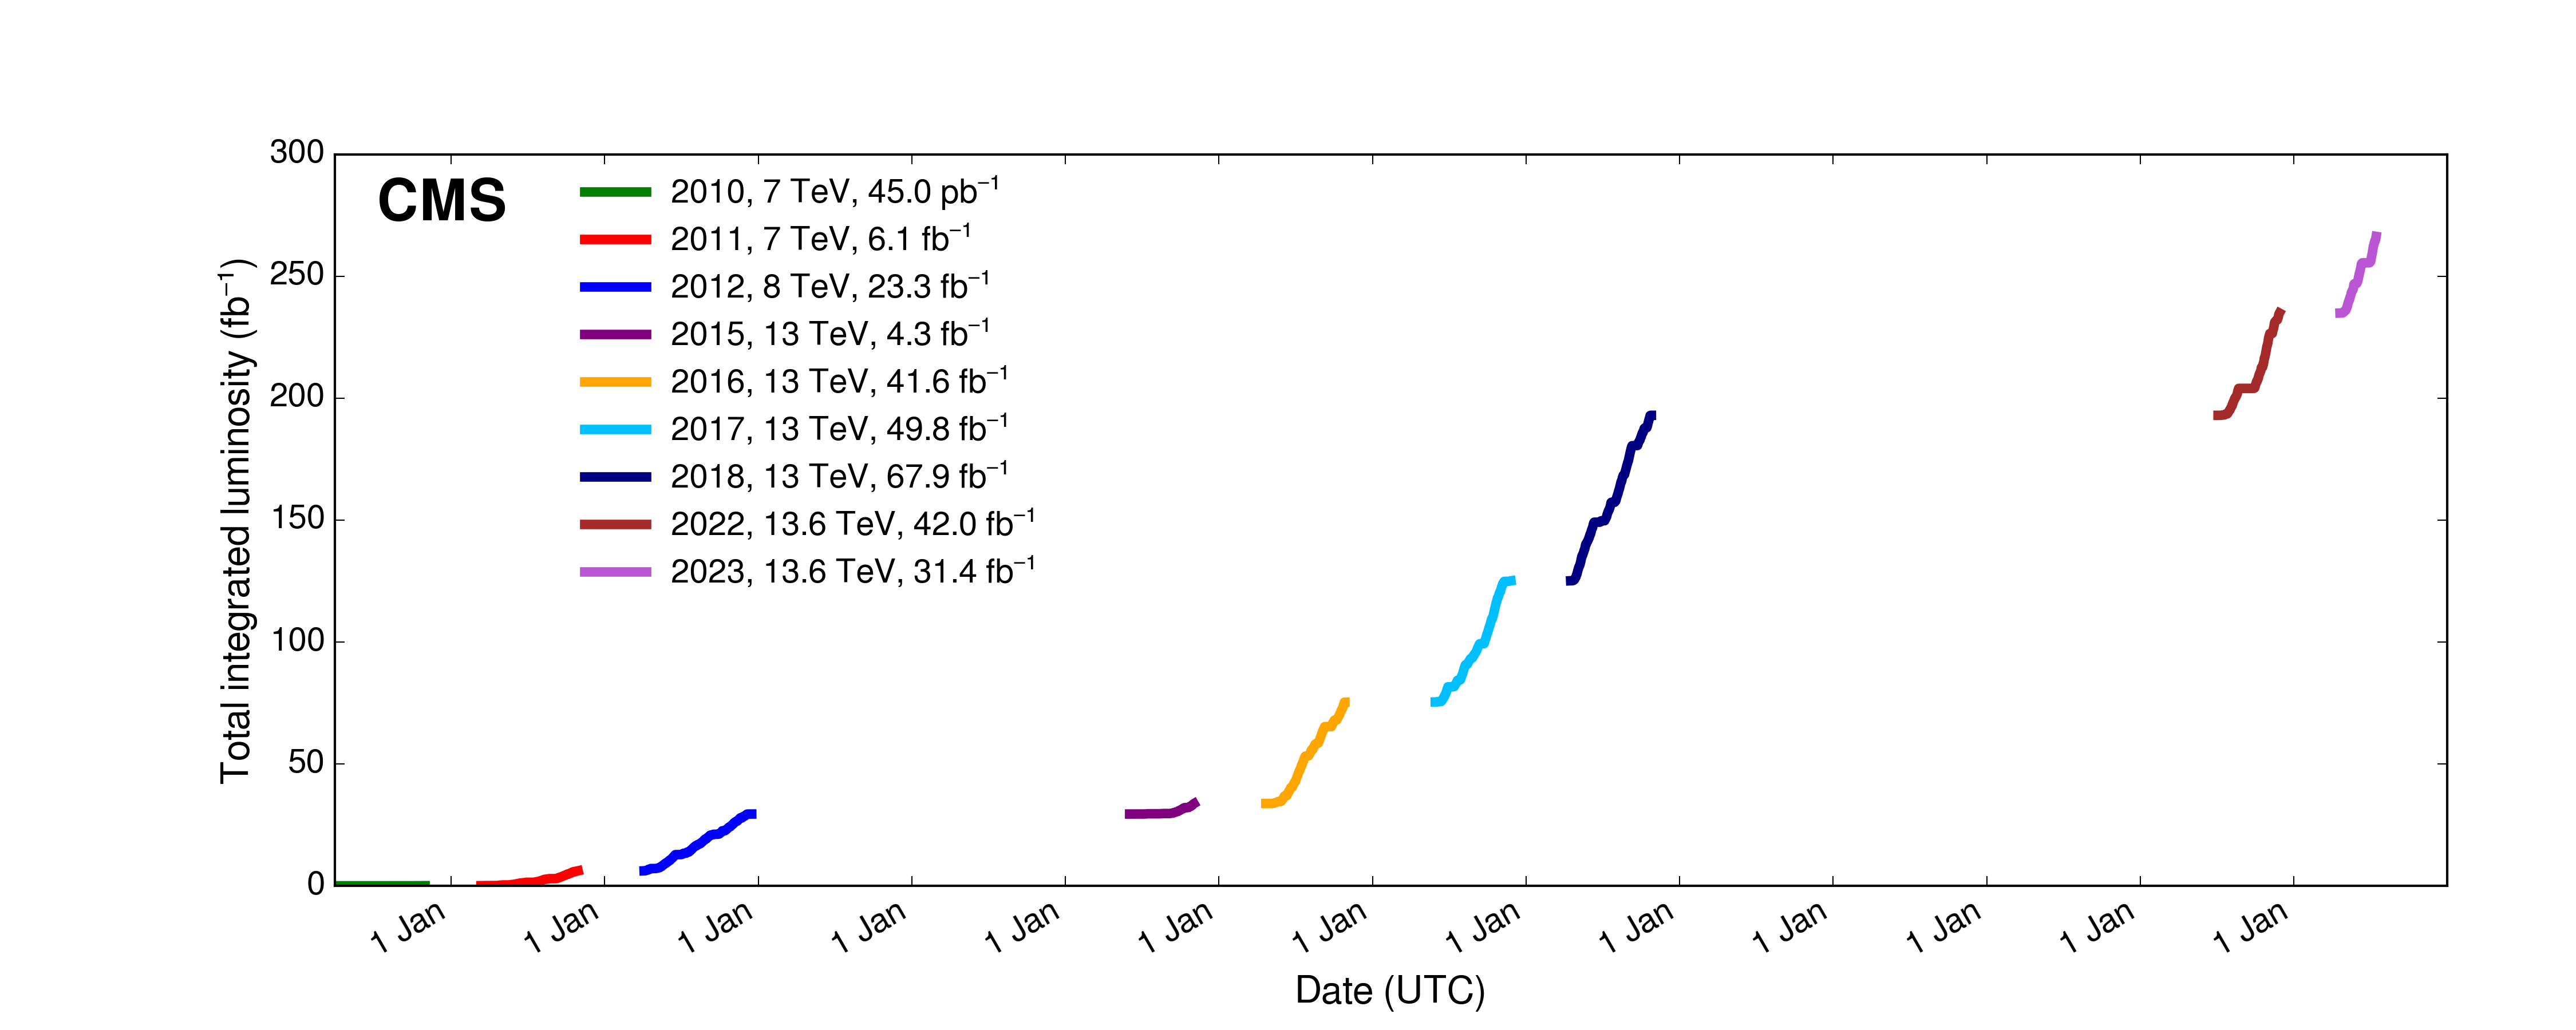
\includegraphics[scale=0.4]{Chapitre3/Images/int_lumi_cumulative_pp_3.png} 
\caption{Luminosité intégrée au cours du temps enregistrée par CMS depuis le lancement du LHC à juillet 2023 \cite{LumiTwiki}.}
\label{lumi}
\end{figure}


\begin{equation}
    \mathcal{L}=\frac{N_pn_bf}{4\pi\sigma_x\sigma_y}F,
\end{equation}

où $N_p$ désigne le nombre de particules par paquets, $n_b$ le nombre de paquets par faisceau, $f$ la fréquence de croisement des faisceaux, $\sigma_{x,y}$ la taille transverse du faisceau selon la coordonnée $x$ ou $y$ et $F$ un correctif lié à l'angle de croisement des faisceaux au point d'interaction. La luminosité instantanée intervient naturellement dans le nombre d'évènements produits au cours du temps selon la formule : 

\begin{equation}
    \frac{\partial N}{\partial t}=\mathcal{L}\times\sigma,
\end{equation}

où $\sigma$ est la section efficace du processus considéré. L'intégration de la luminosité instantanée sur un temps $t$ permet également de connaître la quantité de données enregistrée sur cette période (Fig. \ref{lumi}).  \\

\begin{figure}
\centering
    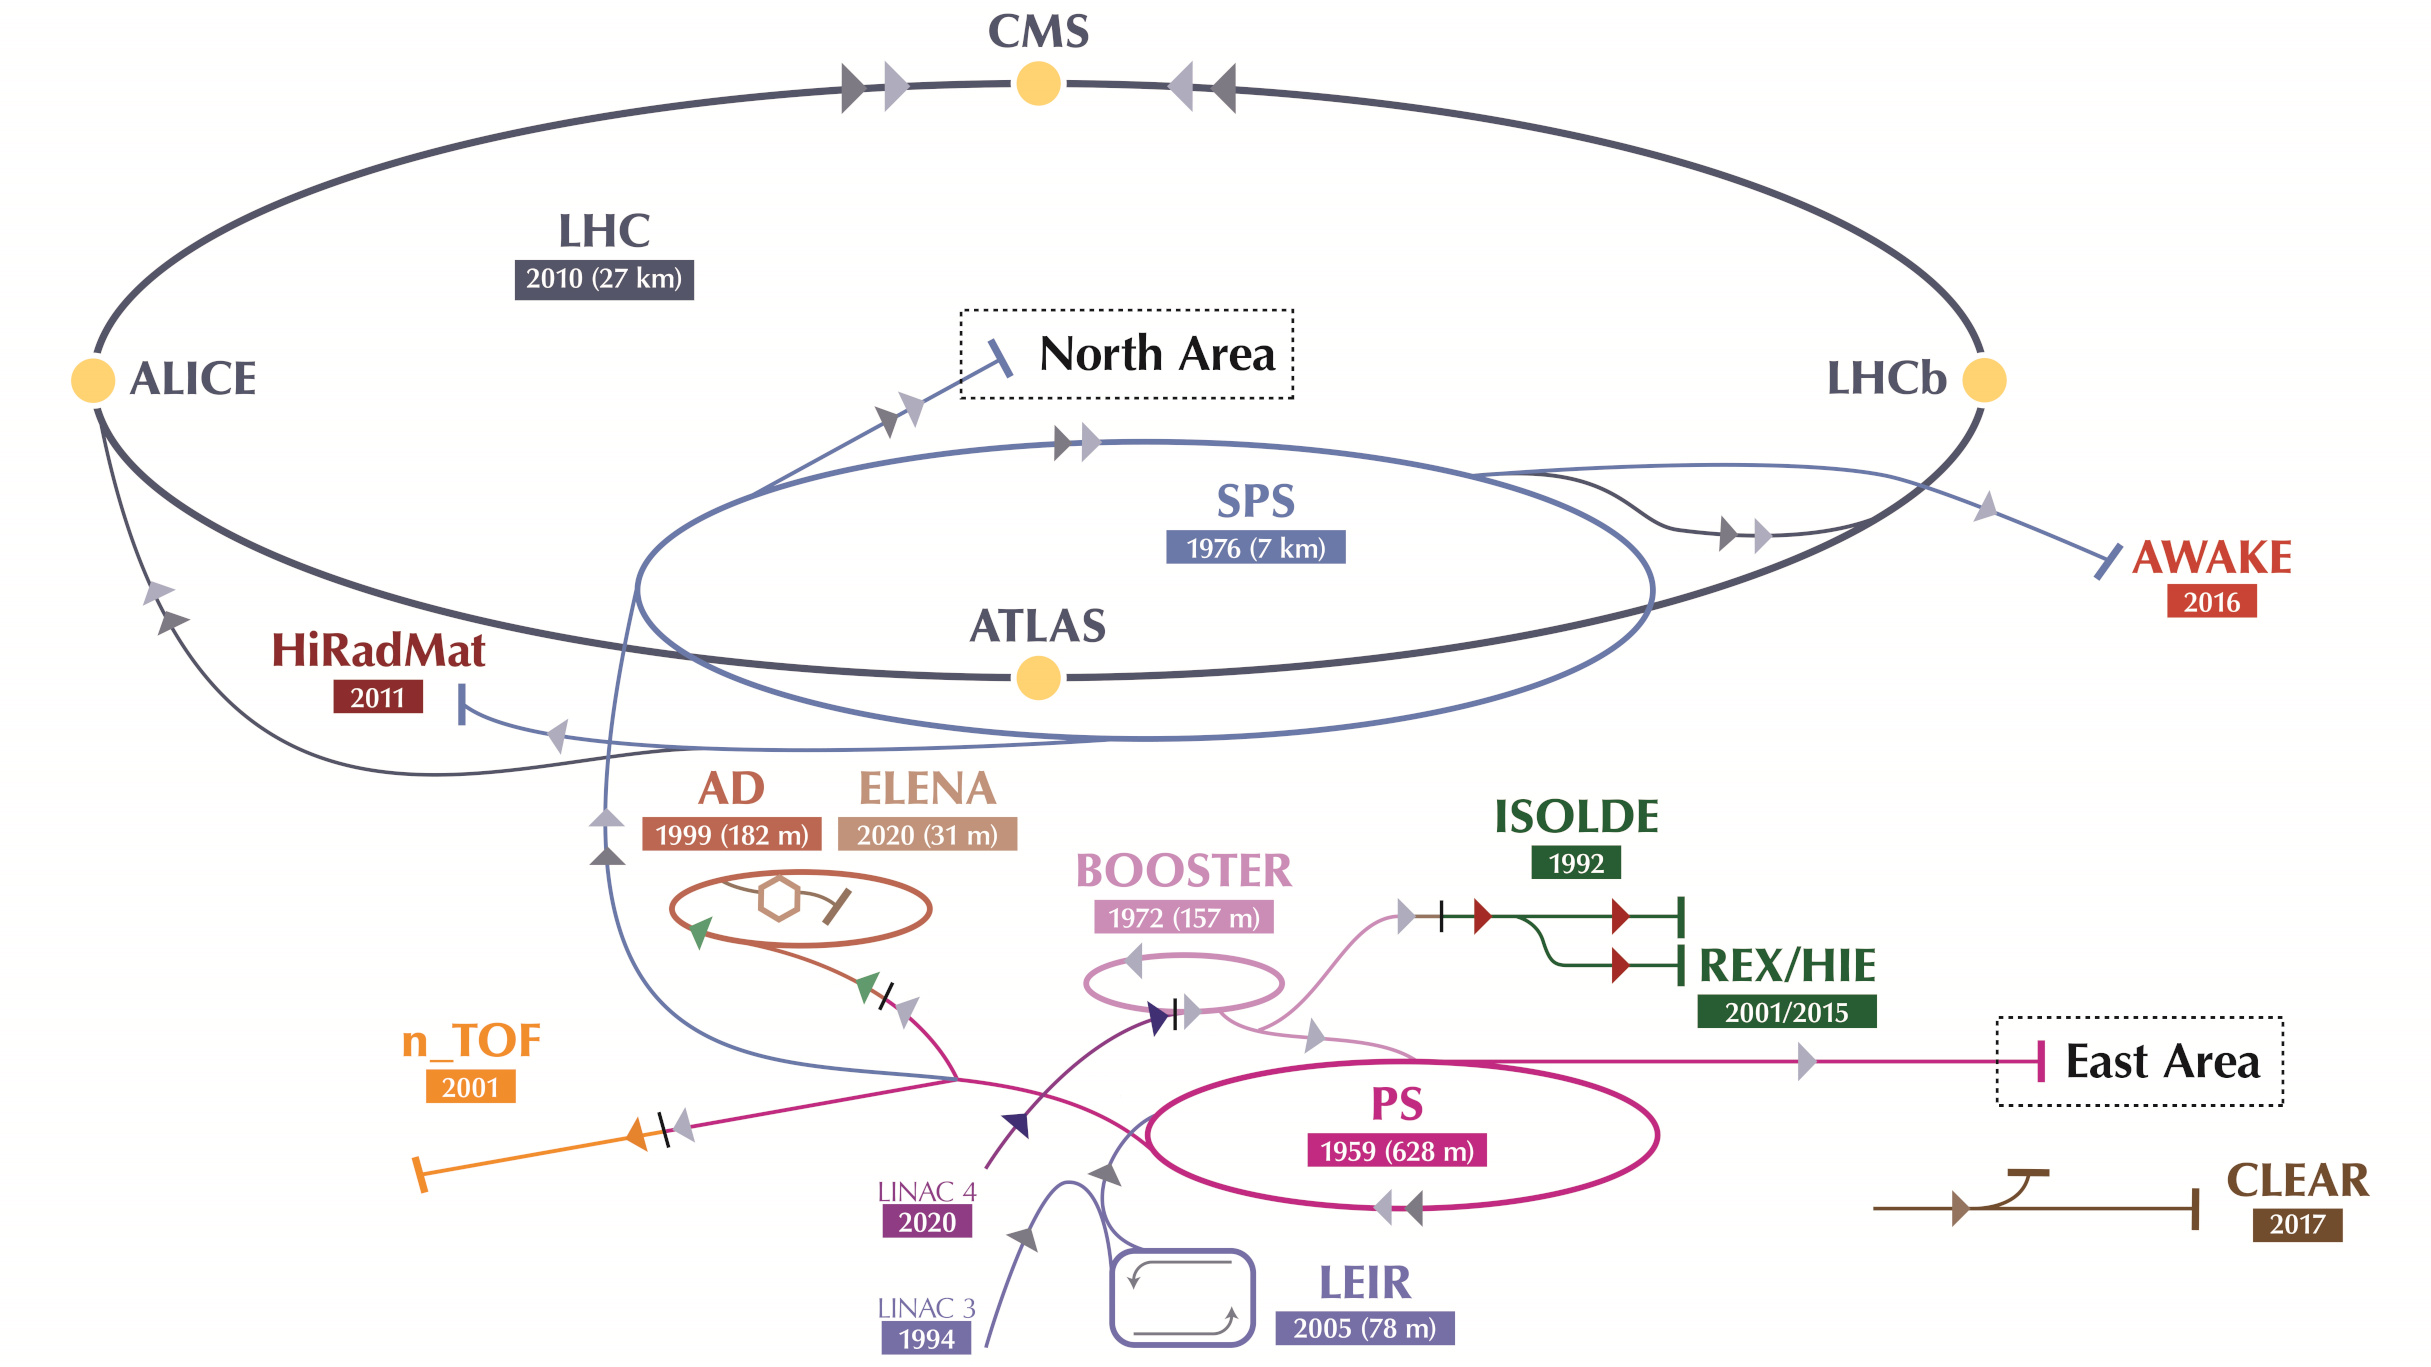
\includegraphics[scale=0.18]{Chapitre3/Images/cern-complex.jpg} 
\caption{Complexe d'accélérateurs du CERN \cite{CERNacc}.}
\label{complex}
\end{figure}

Le LHC est constitué d'une succession de 9593 électroaimants supraconducteurs parmis lesquels se trouvent 1232 aimants dipolaires de courbure fournissant chacun un champ magnétique de $8,3$ T. Chaque élément dipolaire mesure $15$ m et permet une courbure du faisceau de $0,6$ mm/m. Tout au long du parcours, 392 aimants quadripolaires assurent également la focalisation des faisceaux. Le régime supraconducteur des aimants, nécessitant une température de fonctionnement de $1,9$ K ($-271,3~^\circ$C) et un courant nominal de $12~000$ A, est maintenu grâce à un système de refroidissement cryogénique à l'hélium. Chaque faisceau circule dans un tube (\textit{beampipe}) distinct où un ultra vide correspondant à une pression de l'ordre de $10^{-13}$ atm est réalisé. Une fois l'énergie nominale atteinte, les faisceaux entrent en collision en quatre points correspondants aux emplacements des quatre grandes expériences du LHC. Lors de la première phase d'exploitation (Run 1) entre 2009 et 2012, l'énergie de collision dans le centre de masse était de $7$ TeV puis $8$ TeV avec un espacement des paquets de $50$ ns. Lors du Run 2 entre 2015 et 2018, l'énergie de collision a été augmentée à une valeur nominale de $13$ TeV et l'espacement réduit à $25$ ns. Enfin depuis le Run 3, l'énergie maximale de $6,8$ TeV par faisceau est atteinte, soit une énergie de collision de $13,6$ TeV. Le croisement de paquets de protons entraîne également l'apparition d'un phénomène d'empilement (PU, \textit{pile-up} désignant toutes les interactions secondaires prenant place conjointement à l'interaction principale (Fig. \ref{PU}). L'augmentation de la luminosité entraîne naturellement l'augmentation de l'empilement dont la valeur moyenne en juillet 2023 (Run 3) est de 49. \\

\begin{figure}
\centering
    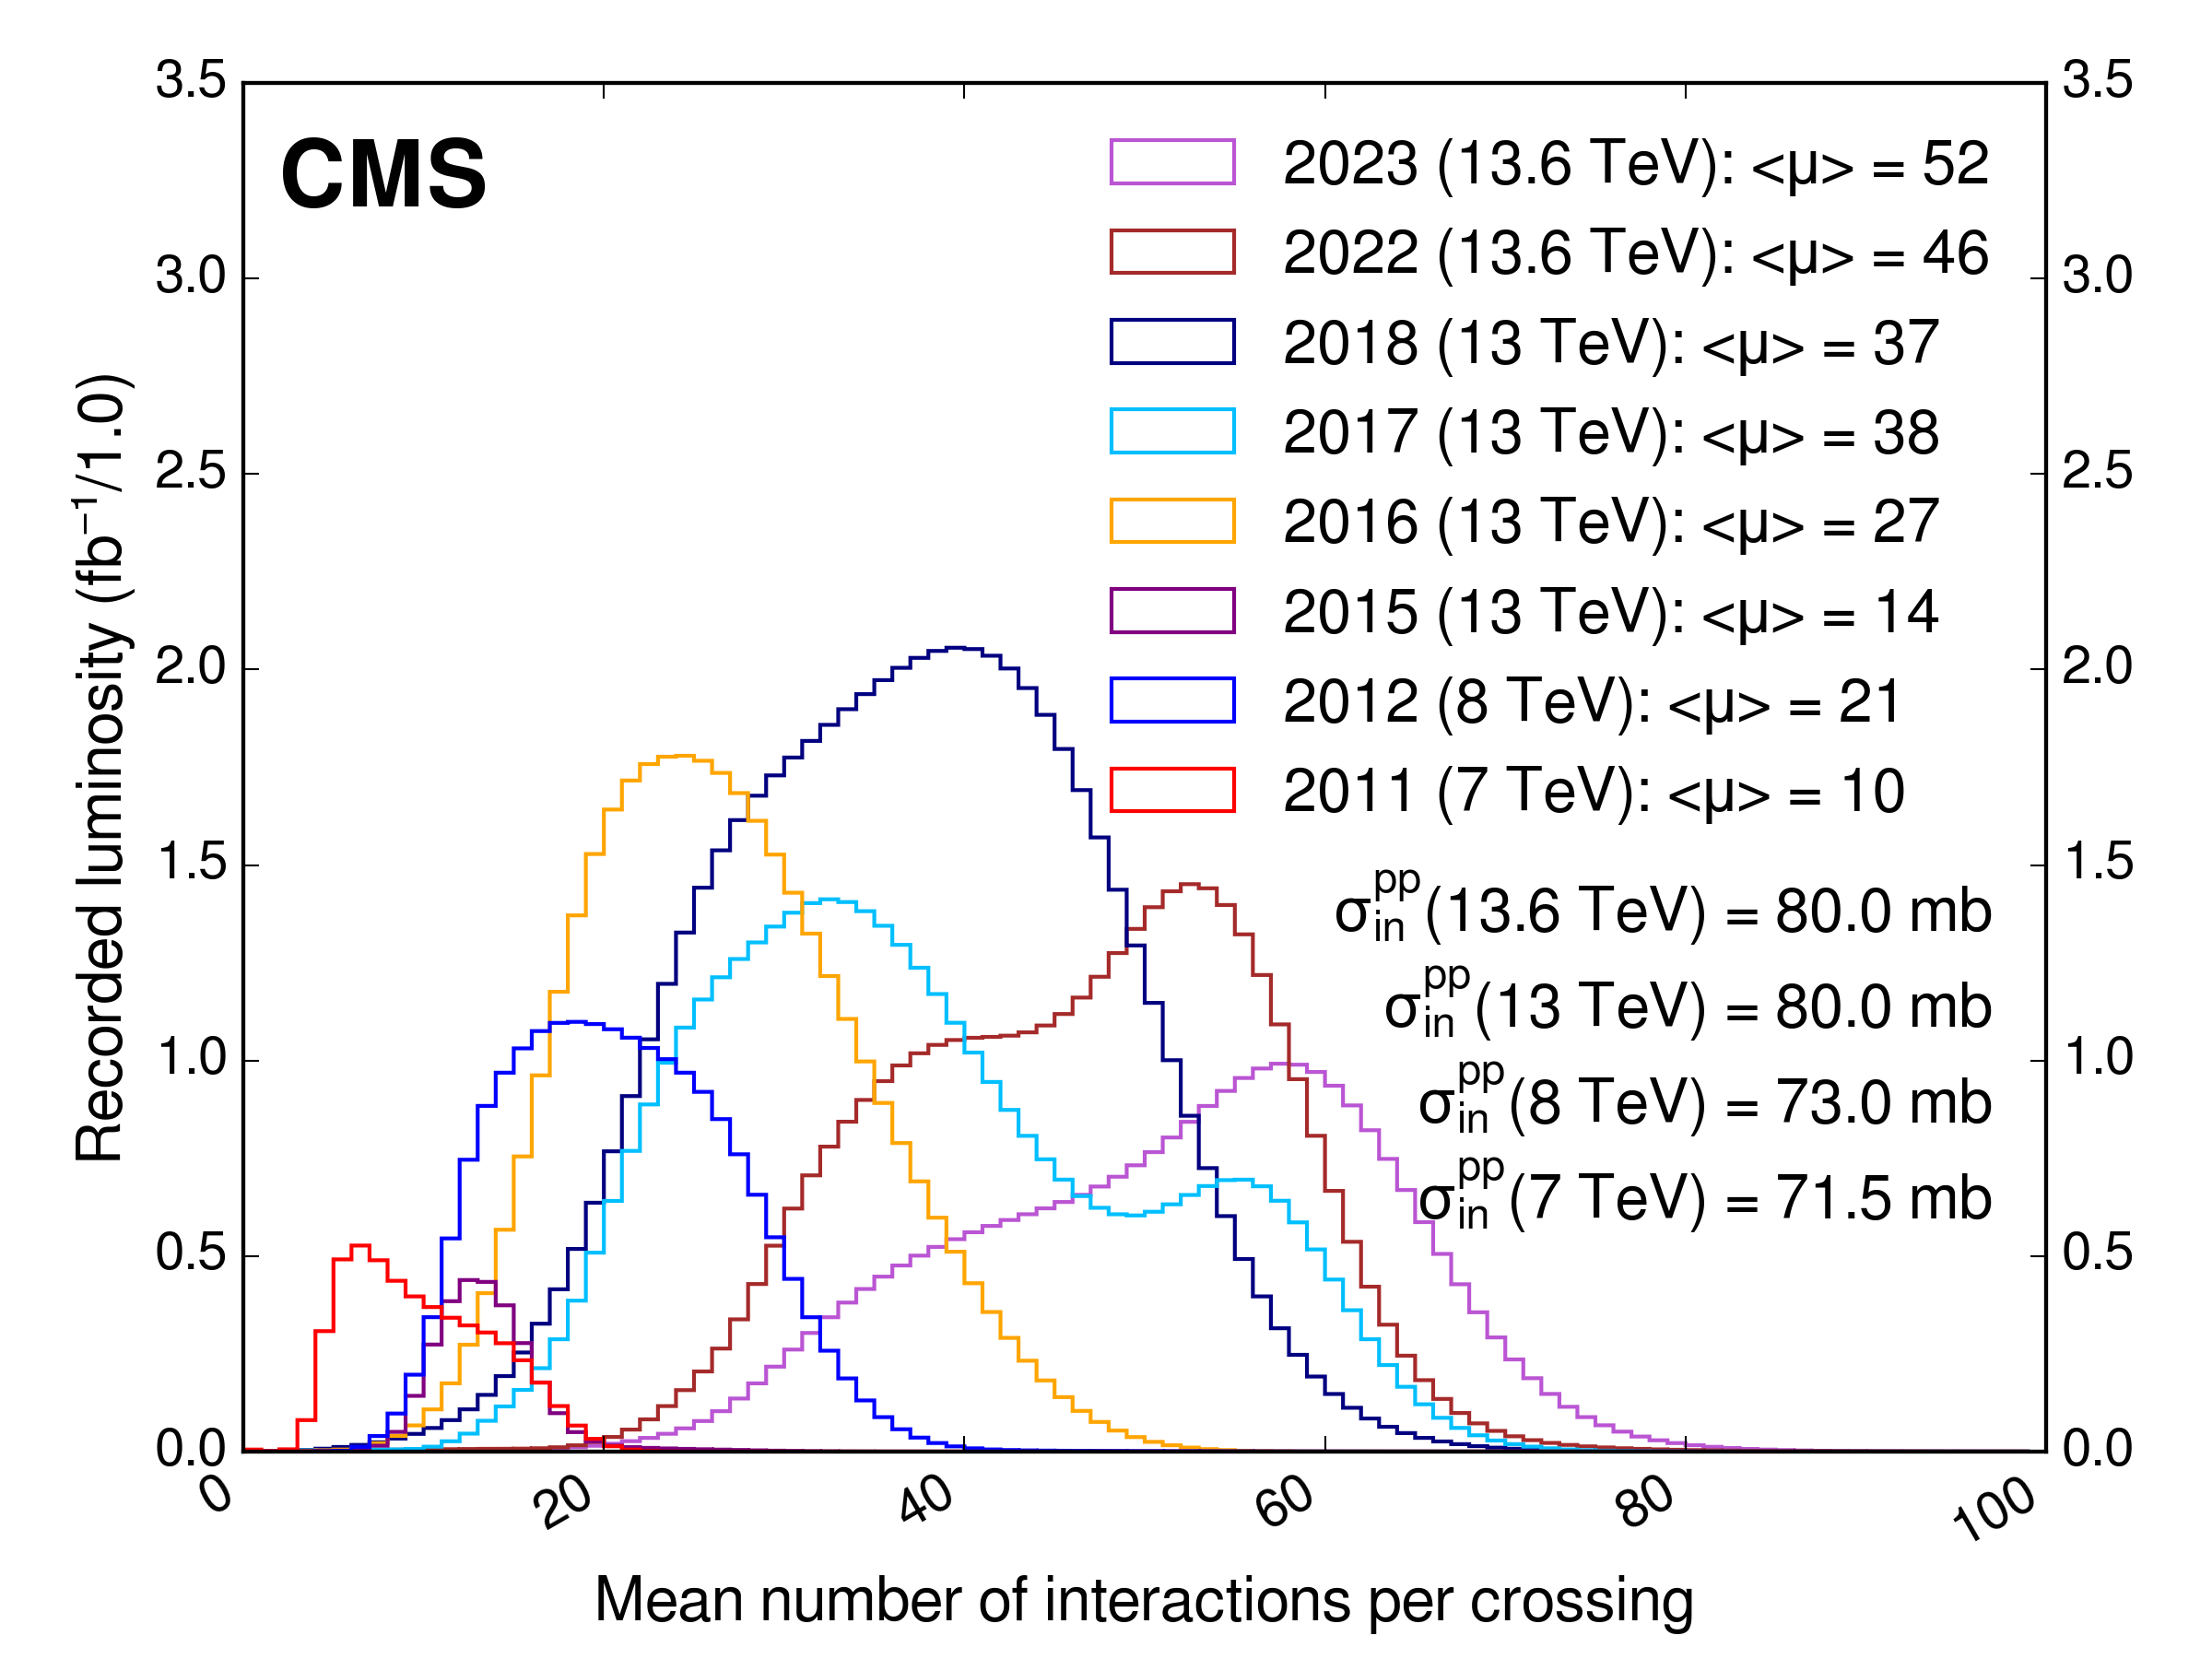
\includegraphics[scale=0.5]{Chapitre3/Images/pileup_allYears.png} 
\caption{Valeur moyenne de l'empilement par croisement de paquets de protons pour toutes les années d'exploitation du LHC \cite{LumiTwiki}.}
\label{PU}
\end{figure}

\section{Détecteur CMS, \textit{\uppercase{C}ompact \uppercase{M}uon \uppercase{S}olenoid}}

Le détecteur CMS, acronyme de \textit{Compact Muon Solenoid}, est un détecteur généraliste de forme cylindrique d'un diamètre de $15$ m et d'une longueur de $22$ m pour un poids total de $14~500$ t. Il est constitué de plusieurs sous-détecteurs et d'un aimant supraconducteur, disposés en couches concentriques (Fig. \ref{cms}), au centre desquelles le LHC délivre ses collisions. \\

\begin{figure}
\centering
    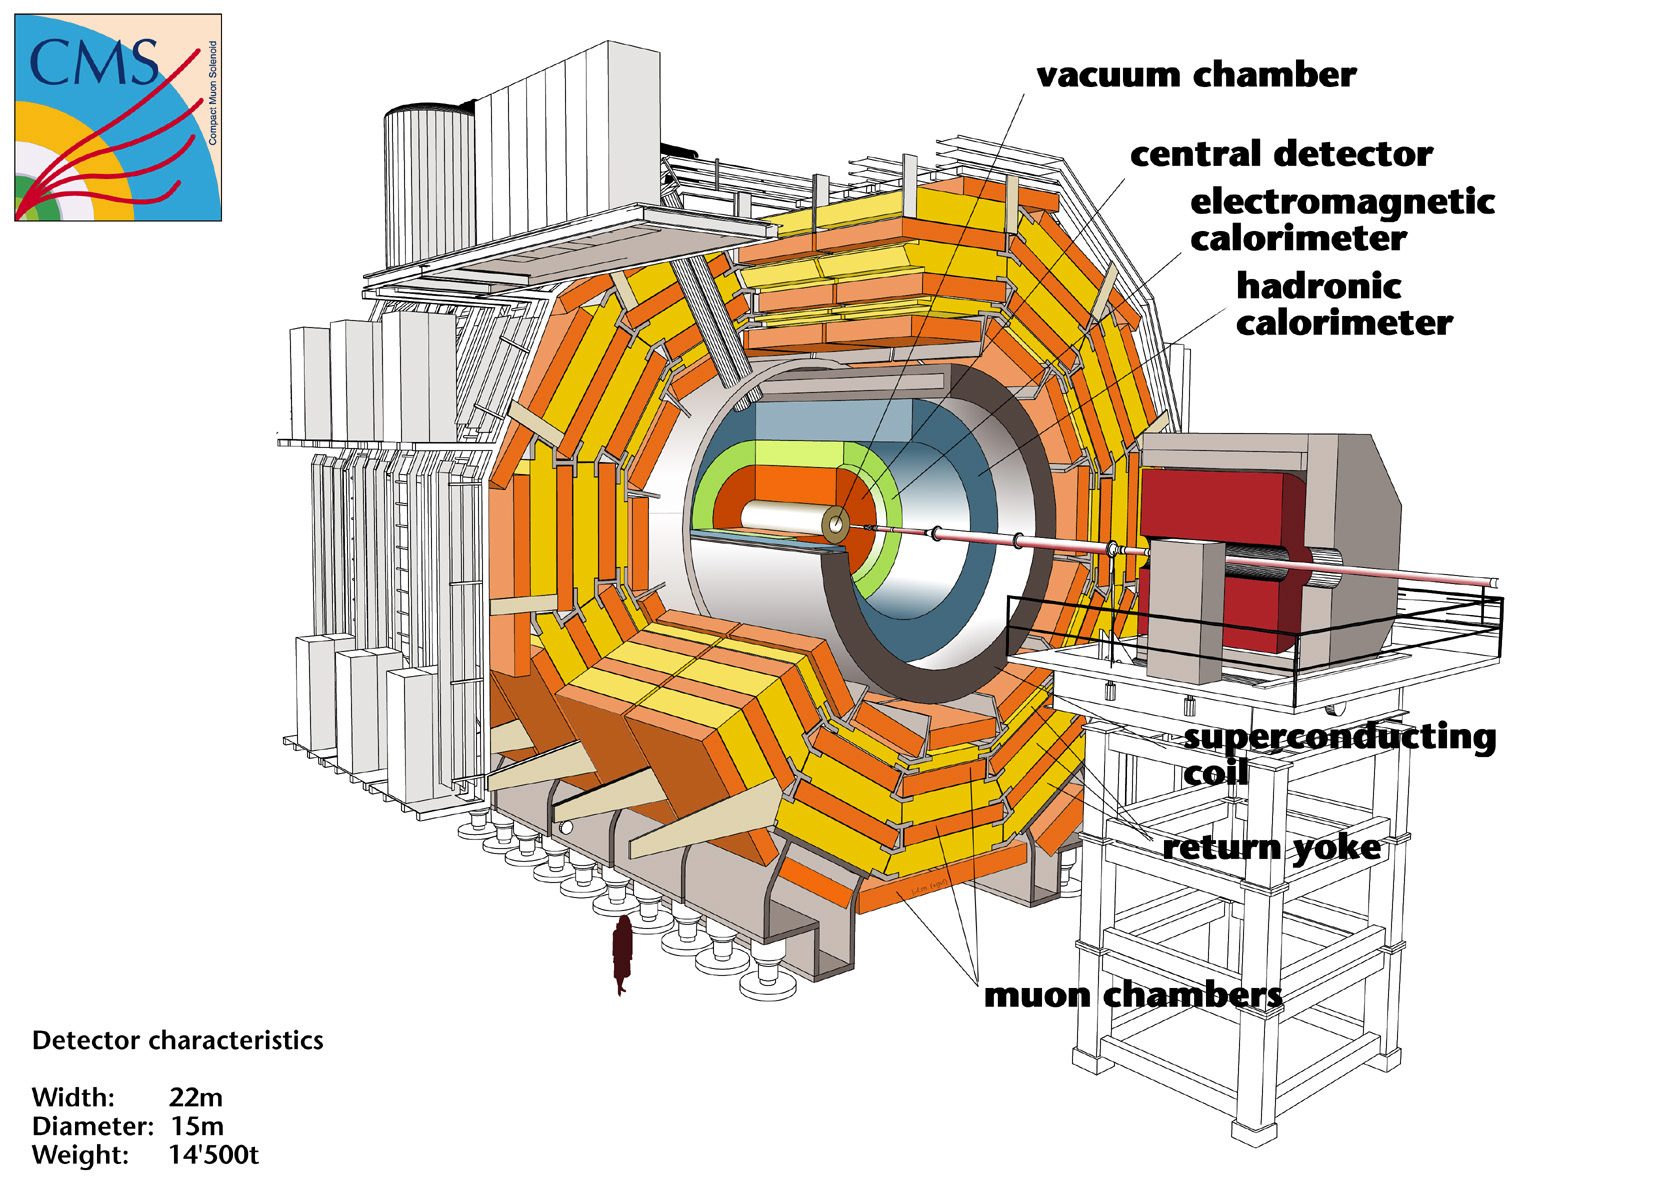
\includegraphics[scale=0.5]{Chapitre3/Images/CMS.jpg} 
\caption{Vue interne du détecteur CMS et de ses différents sous-détecteurs \cite{CMSscheme}.}
\label{cms}
\end{figure}

L'objectif d'un détecteur généraliste tel que CMS est de reconstruire et d'identifier une grande variété de particules issues des collisions produites en son centre. Les particules chargées sont identifiées à l'aide d'un champ magnétique de $3,8$ T fourni par un aimant solénoïde supraconducteur qui courbe leur trajectoire et par un système de trajectographie en silicium placé au centre du détecteur permettant de mesurer leur trajectoire et leur impulsion. L'énergie des particules neutres et chargées est mesurée grâce à un système de calorimétrie constitué d'un calorimètre électromagnétique (ECAL) et hadronique (HCAL). Enfin, CMS dispose d'un large système de trajectographie sur ses couches les plus externes dédié à l'identification et à la reconstruction des muons. 

\subsection{Système de coordonnées}

L'origine du système de coordonnnées de CMS (Fig. \ref{coordinates}) est défini au point d'interaction des faisceaux. L'axe $x$ pointe vers le centre de l'anneau du LHC, l'axe $y$ vers la surface terrestre et l'axe $z$ est orienté selon la direction du faisceau circulant en sens anti-horaire. Pour un vecteur d'impulsion $\vec{p}$ arbitraire, l'angle azimuthal $\phi$ désigne l'angle défini sur l'intervalle $[0;2\pi]$ entre la projection de $\vec{p}$ dans le plan $x$-$y$ et l'axe $x$. L'angle polaire $\theta$ désigne l'angle défini sur l'intervalle $[-\pi;\pi]$ entre $\vec{p}$ et l'axe $z$. Il est toutefois plus courant d'employer la pseudo-rapidité $\eta$ :

$$\eta = -\ln\bigl(\tan\frac{\theta}{2}\bigr).$$

Cette coordonnée est définie sur l'intervalle $]-\infty;+\infty[$, où chaque borne correspond à la direction selon l'axe $\pm z$, $\eta=0$ correspond à la direction selon l'axe $y$, et la différence $\Delta \eta$ entre deux particules est invariante de Lorentz. La pseudo-rapidité rentre également dans la définition de la séparation spatiale $\Delta R$ entre deux particules ou objets dans le plan $\eta$-$\phi$ définie comme :

$$\Delta R = \sqrt{\Delta\phi^2+\Delta\eta^2}.$$

La nature composite du proton ne permet pas de connaître l'impulsion selon l'axe $z$ des partons mis en jeu lors des collisions. En revanche cette impulsion est négligeable dans le plan transverse, et il convient ainsi de définir l'impulsion transverse : 

$$p_T=\sqrt{p_x^2+p_y^2},$$

dont la somme vectorielle $\Sigma\vec{p}_T^i$ sur chacune des particules $i$ de l'état final pour une collision donnée doit être nulle par conservation. Certaines particules comme le neutrino étant indétectables au sein du détecteur, on définit également l'impulsion transverse manquante :

$$\vec{p}^{miss}_T=-\Sigma\vec{p}_T^i,$$

correspondant à l'impulsion transverse totale des particules non observées. Aux régimes de haute énergie où la masse d'une particule est négligeable devant son impulsion, l'énergie transverse manquante $E^{miss}_T$, plus couramment désignée sous l'acronyme MET (\textit{Missing $E_T$}), s'exprime selon la relation :

$$E^{miss}_T=|p_T^{miss}|^2.$$

\colorlet{veccol}{green!50!black}
\colorlet{myred}{red!70!black}
\colorlet{myblue}{blue!70!black}
\colorlet{mydarkred}{red!40!black}
\colorlet{mydarkblue}{blue!30!black}
\colorlet{CMScol}{red!80!black}
\colorlet{ATLAScol}{blue!80!black}
\tikzset{>=latex} % for LaTeX arrow head
\tikzstyle{axis}=[->,thick,line cap=round]
\tikzstyle{detector}=[thick,draw=mydarkred,rotate around z=\ang]
\tikzstyle{beam pipe}=[draw=blue!20!black!50,fill=blue!20!black!10,rotate around z=\ang]
\tikzstyle{detector surface}=[red!60!black!60,opacity=0.06,rotate around z=\ang]
\usetikzlibrary{angles,quotes} % for pic (angle labels)
\usetikzlibrary{bending} % for arrow head angle
%\newcommand*{\vv}[1]{\vec{\mkern0mu#1}} % aligned vector arrow

% CMS detector - left perspective
\tdplotsetmaincoords{75}{50} % to reset previous setting
\begin{figure}
\begin{tikzpicture}[scale=2.8,tdplot_main_coords,rotate around x=90]
  
  % VARIABLES
  \def\rvec{\L/2/cos(\thetavec)}
  \def\thetavec{18}
  \def\phivec{60}
  \def\L{3.3}    % detector length
  \def\R{0.75}   % detector cylinder radius
  \def\l{4.3}    % beam pipe length
  \def\r{0.04}   % beam pipe radius
  \def\rt{0.042} % beam pipe radius + line thickness
  \def\xmax{1}   % maximum x axis
  \def\ymax{1}   % maximum y axis
  \def\zmin{-\l/2-0.2} % minimum z axis
  \def\zmax{\l/2+0.3}  % maximum z axis
  \def\w{0.3}
  \coordinate (O) at (0,0,0);
  \coordinate (Z) at (0,0,\L/2);
  \tdplotsetcoord{O'}{0.022}{\thetavec}{\phivec} % slightly shifted origin
  \tdplotsetcoord{O''}{0.018}{90}{\phivec} % slightly shifted origin
  \tdplotsetcoord{P}{\rvec}{\thetavec}{\phivec}
  
  % CYLINDER behind
  \def\ang{19} % rotate lines to simulate cylinder
  \fill[top color=red!50!black!4,bottom color=red!60!black!2,rotate around z=\ang]
    (0,\R,\L/2) --++ (0,0,-\L) arc(90:270:\R) --++ (0,0,\L) arc(270:90:\R) -- cycle;
  \fill[detector surface] % transverse plane at z=L/2
    (0,0,\L/2) --++ (0,\R,0) arc(90:270:\R) -- cycle;
  \fill[detector surface] % transverse plane at z=-L/2
    (0,0,-\L/2) --++ (0,\R,0) arc(90:270:\R) -- cycle;
  \tdplotdrawarc[detector]{(0,0,\L/2)}{\R}{0}{360}{}{}
  \tdplotdrawarc[detector,thin]{(0,0,-\L/2)}{\R}{0}{360}{}{}
  %\draw[detector,canvas is yx plane at z=-\L/2] (0,0,0) circle(\R);
  \draw[detector,thin] % transverse plane at z=0
    (90-\ang:\R) arc (90-\ang:270:\R);
  \draw[detector] (0,0,-\L/2)++(90:\R) --++ (0,0,\L); % top horizontal
  \draw[detector] (0,0,-\L/2)++(-90:\R) --++ (0,0,\L); % bottom horizontal
  
  % BEAM PIPE
  \tdplotdrawarc[beam pipe]{(0,0,\l/2)}{\r}{0}{360}{}{}
  %\tdplotdrawarc[beam pipe]{(0,0,-\l/2)}{\r}{\ang-90}{90}{}{}
  %\draw[beam pipe] % cylindric beam pipe
  %  (0,\r,-\l/2) --++ (0,0,\l) arc(90:-90:\r)
  %  --++ (0,0,-\l) arc(-90:90:\r);
  \draw[beam pipe] % beam pipe, thinner in middle
    (0,\r,-\l/2) -- (0,\r,-0.2*\l) -- (90:0.5*\r)
    -- (0,\r,0.2*\l) -- (0,\r,0.5*\l) arc(90:-90:\r)
    -- (0,-\r,0.2*\l) -- (-90:0.5*\r) --
    (0,-\r,-0.2*\l) -- (0,-\r,-\l/2) arc(-90:90:\r);
  \draw[beam pipe] (0,0,\l/2) circle(\r);
  
  % AXES
  %\draw[thick,->] (0,0,0) -- (0,0,1) node[below right]{$z$}; % short
  \draw[axis,-] (0,0,\zmin) -- (0,0,0); % long
  \fill[CMScol] (O) circle(0.5pt) node[right=1,below=1] {};
  \draw[axis] (0,0,0.020) -- (0,0,\zmax) node[right=3,below=1]{$z$}; % long
  \draw[axis] (0,0.019,0) -- (0,\ymax,0) node[below left]{$y$};
  \draw[dashed,myred] (Px)  -- (Pxy);
  \draw[axis] (0.022,0,0) -- (\xmax,0,0) node[below=1,right=-2]{$x$};
  
  % LABELS
  \node[mydarkred,above] at (0,\ymax,0) {$\eta=0$};
  \node[mydarkred,above=3] at (0,\R,0.3*\L) {$\eta>0$};
  \node[mydarkred,above=3] at (0,\R,-0.2*\L) {$\eta<0$};
  \node[mydarkred,below=1,left] at (0,0,\zmax) {$\eta=\infty$};
  \node[mydarkred,above=1,right] at (0,0,\zmin) {$\eta=-\infty$};
  
  % VECTORS
  %\fill[radius=0.4,red] (P) circle;
  \draw[dashed,myred] (P)  -- (Pxy);
  \draw[dashed,myred] (Py) -- (Pxy);
  \draw[dashed,myred] (P) -- (Pz);
  \draw[->,red,line cap=round] (O') -- (P) node[anchor=-30] {$\vv{p}$};
  \draw[->,red,line cap=round] (O') -- (Pxy) node[anchor=-70] {$\vv{p}_{T}$};
  
  % CYLINDER front
  \draw[beam pipe,fill=none] (0,\r,-\l/2) arc(90:-90:\r);
  \fill[detector surface] % transverse plane at z=L/2
    (0,\rt,\L/2) --++ (0,\R-\rt,0) arc(90:-90:\R) --++ (0,\R-\rt,0) arc(-90:90:\rt);
  \fill[detector surface] % transverse plane at z=-L/2
    (0,\rt,-\L/2) --++ (0,\R-\rt,0) arc(90:-90:\R) --++ (0,\R-\rt,0) arc(-90:90:\rt);
  \tdplotdrawarc[detector]{(0,0,\L/2)}{\R}{-90}{90}{}{} % transverse plane at z=L/2
  \tdplotdrawarc[detector]{(0,0,-\L/2)}{\R}{-90}{90}{}{} % transverse plane at z=-L/2
  \draw[beam pipe,fill=none] (0,\r,\l/2) arc(90:-90:\r);
  \draw[detector,very thin] % transverse plane at z=0
    (90-\ang:\R) arc (90-\ang:-90:\R);
  
  % ANGLES
  \tdplotdrawarc[thick,red!57!black!3] % contour
    {(O)}{0.2}{4}{0.7*\phivec}{}{}
  \tdplotdrawarc[draw=none,opacity=0.8]{(O)}{0.2}{0}{\phivec} % transparant contour
    {above=2,right=-1,anchor=mid west}{\contour{red!55!black!3}{$\phi$}}
  \tdplotdrawarc[->]{(O)}{0.2}{0}{\phivec}
    {above=2,right=-1,anchor=mid west}{$\phi$}
  \tdplotdrawarc[->,rotate around z=\phivec-90,rotate around y=-90]
    {(O)}{0.88}{0}{\thetavec}{anchor=mid east}{$\theta$}
  \tdplotdrawarc[thick,red!58!black!4,rotate around z=\phivec-90,rotate around y=-90] % contour
    {(O)}{0.3}{88}{0.5*(90+\thetavec)}{}{}
  \tdplotdrawarc[-{>[flex'=1]},rotate around z=\phivec-90,rotate around y=-90,line cap=round]
    {(O)}{0.3}{90}{\thetavec}{above=4,right=2,anchor=mid east}{$\eta$}
  \draw[mydarkred] (0,0,\L/2) --++ (\R,0,0);
  \tdplotdrawarc[thick,red!60!black!6] % contour
    {(Z)}{0.2}{4}{0.7*\phivec}{}{}
  \tdplotdrawarc[draw=none,opacity=0.8]{(Z)}{0.2}{0}{\phivec} % transparant contour
    {above=2,right=-1,anchor=mid west}{\contour{red!60!black!6}{$\phi$}}
  \tdplotdrawarc[->]{(Z)}{0.2}{0}{\phivec}
    {above=2,right=-1,anchor=mid west}{$\phi$}
  
  % COMPASS - CMS-ATLAS axis has a ~12° declination
  \draw[->,thick,orange!30!black] (1.4*\w,-\R,-0.1*\L) --++ (2*\w,0,0)
    node[below=1,right,scale=0.8,align=center] {center of\\[-1pt]the LHC};

\end{tikzpicture}
\caption{Système de coordonnées du détecteur CMS \cite{izaak}.}
\label{coordinates}
\end{figure}


\subsection{Aimant supraconducteur}

L'aimant supraconducteur de CMS est un aimant solénoïde cylindrique d'un rayon de $6$ m et d'une longueur de $12,5$ m qui englobe au son centre le trajectographe en silicium et les calorimètres. Il est capable de délivrer un champ magnétique nominal de $3,8$ T et permet de courber la trajectoire des particules chargées afin d'en mesurer l'impulsion et la charge électrique. L'aimant et son champ magnétique sont eux mêmes confinés dans une culasse en fer permettant de créer un champ magnétique externe de $1,8$ T dans lequel se trouvent les chambres à muons. Le régime supraconducteur est maintenu grâce à un système de refroidissement à l'hélium liquide et une cuve à vide dans laquelle règne une température de $4,1$ K.

\subsection{Trajectographe en silicium}

La méthode de détection et de reconstruction de la trace des particules chargées dans le trajectographe de CMS, dont le détail est donné dans la section \ref{PF}, repose sur les propriétés de semi-conducteur du silicium. Par définition, un semi-conducteur est un matériau isolant dont l'écart modéré d'énergie entre sa bande de valence et sa bande de conduction permet le passage de courant sous certaines conditions. En particulier, l'énergie déposée par le passage d'une particule ionisante au sein d'un semi-conducteur peut suffire à la formation d'une paire électron-trou pouvant générer un courant par application d'un champ électrique externe. Dans le cas du silicium l'énergie minimale requise pour la formation d'une paire électron-trou est de $3,6$ eV, ainsi le passage d'une particule au minimum d'ionisation (MIP) entraîne la formation de $80$ paires/$\mu$m. Pour un détecteur d'une épaisseur de $300$ $\mu$m, ce même passage entraînera la formation d'environ $2\times10^4$ électrons, indiscernables parmi une densité de porteurs intrinsèques du silicium d'environ $10^{10}$ cm$^{-3}$. La formation d'une zone de déplétion dépourvue de charges libres au sein du matériau est ainsi cruciale pour permettre la détection de particules chargées. \\

La conductivité du silicium peut être améliorée par une technique de dopage consistant à insérer au sein de sa maille cristalline des atomes étrangers donneurs (type III) ou accepteurs (type V) d'électrons. Lorsqu'un matériau de type III est employé, le silicium est enrichi en électrons et possède un dopage de type $n$. A l'inverse, un matériau de type V entraîne un déficit d'électrons au sein du silicium et constitue un dopage de type $p$. Les détecteurs en silicium sont généralement conçus à partir d'un volume de type $n$ sur lequel une couche de type $p$ sur laquelle les charges sont collectées est déposée. La zone de contact formée constitue une jonction dite $p$-$n$, au niveau de laquelle une zone de déplétion dépourvue de charges se crée par des effets de migration entre les deux couches. Par ailleurs, au sein d'un détecteur, la jonction $p$-$n$ est généralement opérée en régime de polarisation inverse en appliquant un champ électrique généré par une tension externe dont la cathode est reliée au volume $n$ et l'anode à la couche $p$. Cette méthode permet non seulement d'élargir la zone de déplétion qui constitue la zone active du détecteur proportionnellement à la tension appliquée, mais également de prévenir la fuite de charges à l'origine du bruit. Une couche de type $n^+$, plus fortement dopée, peut également être déposée sur la face opposée du volume de type $n$ afin d'augmenter davantage l'effet de déplétion. \\

Le trajectographe de CMS est un cylindre constitué de couches de détection concentriques successives dans sa partie centrale (tonneau), et d'un empilement de disques dans ses parties avants (bouchons) permettant de couvrir la région définie par $r<1,2$m et $|\eta|<2,5$ (Fig. \ref{tracker}). Le détecteur est entièrement équipé de modules en silicium, avec sa partie interne constituée de pixels, et sa partie externe constituée de modules à micro-pistes. \\

\begin{figure}
\centering
    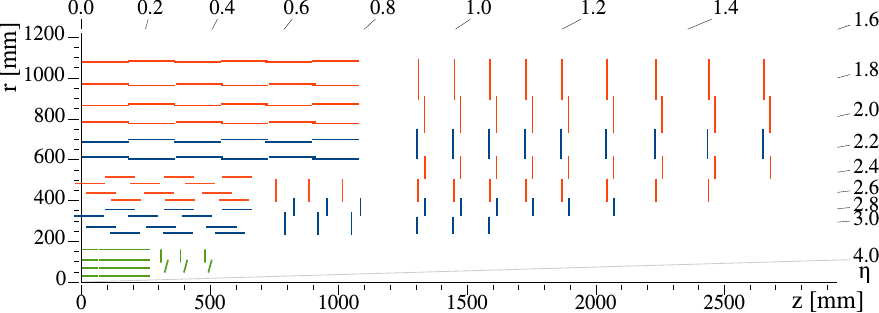
\includegraphics[scale=0.95]{Chapitre3/Images/Phase1_Tracker_1Quarter.png} 
\caption{Quart de coupe dans le plan $r$-$z$ du trajectographe Phase-1 de CMS. Les pixels sont représentés en vert, les modules à pistes simple face en rouge et les modules à pistes double face en bleu \cite{TrackerPerformance}.}
\label{tracker}
\end{figure}

\subsubsection{\ding{95} Trajectographe à pixels}

Les détecteurs à pixels sont constitués d'un volume actif en silicium dopé sur lequel une couche de type inverse et segmentée en "pixels" est déposée. En ajoutant une piste de lecture à chaque segment, les pixels agissent comme des détecteurs individuels et offrent une excellente granularité. Dans le cas de CMS, le volume actif des modules est composé d'un volume de type $n$ surplombé d'une couche de type $n^+$  et d'une couche de type $p$ sur sa face opposée. Une fois opérée en polarisation inverse, cette configuration permet de collecter des électrons sur les pixels plutôt que des trous. Ces derniers possèdent en effet une mobilité plus faible que les électrons et sont ainsi davantage sujets aux effets de capture causés par les dommages liés à la forte exposition aux radiations. En 2017, la Phase-$0$ du trajectographe de CMS s'est achevée pour laisser place à la Phase-$1$ prévue pour être opérée jusqu'à la fin du Run 3. Durant cette phase de jouvence du détecteur, une couche supplémentaire de pixels a été ajoutée dans le tonneau (BPIX, \textit{Barrel Pixels}), portant à 4 le nombre total de couches concentriques situées respectivement à $r=30,68,109,160$ mm. Les bouchons (FPIX, \textit{Forward Pixels}) sont quant à eux constitués de trois disques couvrant la région située dans un rayon compris entre $45$ et $161$ mm. Au total, le trajectographe à pixels est constitué de $1856$ modules silicium pour un total de $100$ millions de pixels d'une taille de $100\times150$ $\mu$m$^2$. La résolution sur la reconstruction des \textit{hits} individuels des traces de particules chargées est de $10$ $\mu$m dans le BPIX et de $15$ $\mu$m dans le FPIX.

\subsubsection{\ding{95} Trajectographe à pistes}

Les modules à micro-pistes sont constitués d'un volume actif de type $n$ sur lequel sont implantées des bandes de type $p^+$. Le trajectographe à pistes est constitué d'une partie interne comprenant un tonneau (TIB, \textit{Tracker Inner Barrel}) constitué de quatre couches, et de deux bouchons (TID, \textit{Tracker Inner Disks}) constitués de trois disques sur les parties avants. Chaque module de la partie interne possède une épaisseur de $320$ $\mu$m et un espacement entre chaque piste de $80$ $\mu$m. La partie externe comporte quant à elle six couches dans son tonneau (TOB, \textit{Tracker Outer Barrel}) et neuf disques dans chacun de ses bouchons (TEC, \textit{Tracker EndCaps}). Les modules de la partie externe possèdent une épaisseur de $500$ $\mu$m et un espacement entre les pistes de $205$ $\mu$m. \\

\begin{figure}
    \begin{subfigure}[b]{0.5\linewidth}
    \centering
    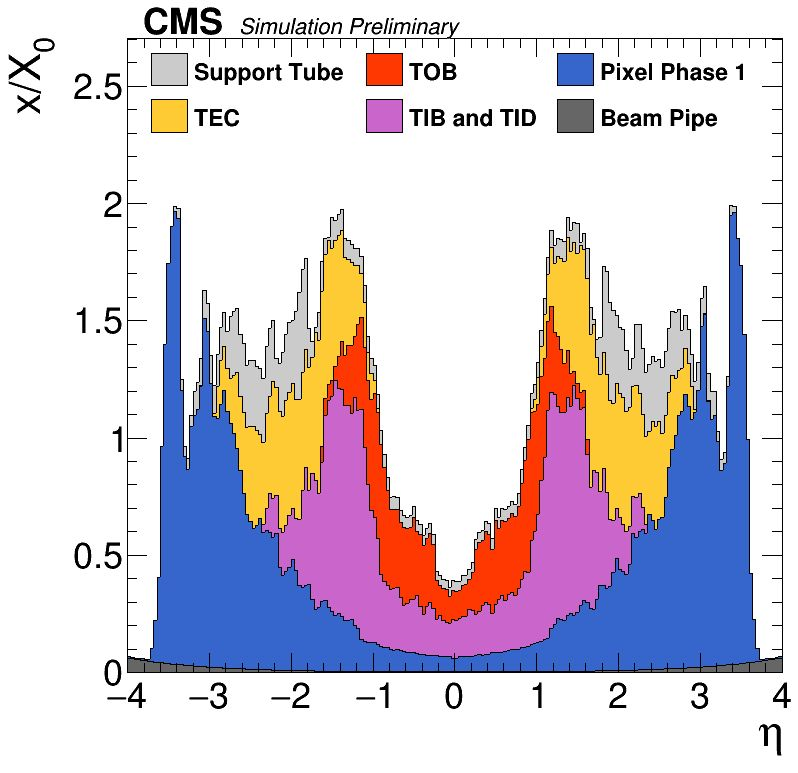
\includegraphics[width=\linewidth]{Chapitre3/Images/MaterialBudgetTrackerPhase1_FractionRadiationLength.png} 
    \caption*{} 
    \vspace{0.5ex}
  \end{subfigure}%% 
  \begin{subfigure}[b]{0.5\linewidth}
    \centering
    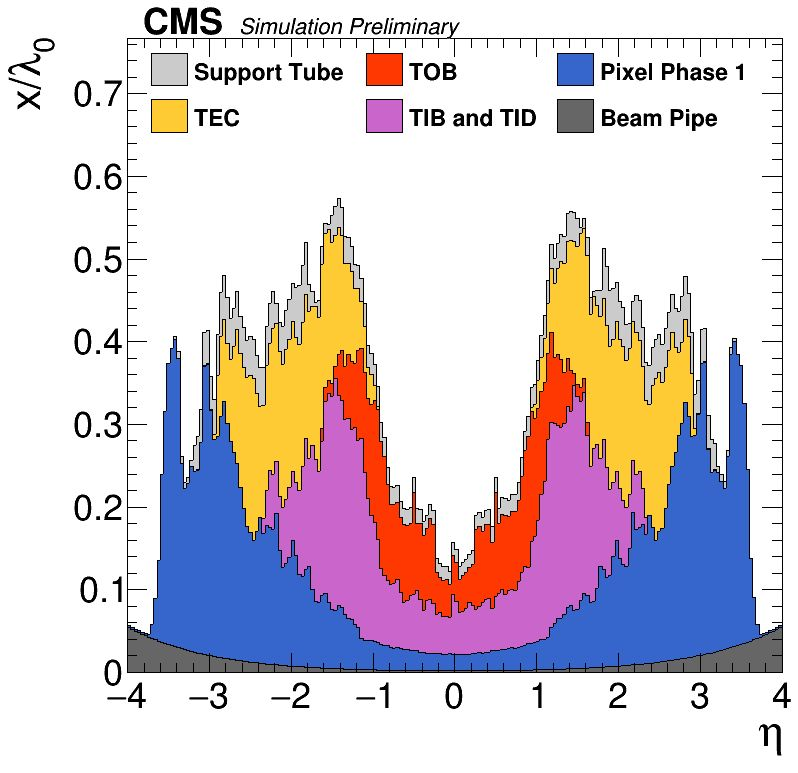
\includegraphics[width=\linewidth]{Chapitre3/Images/MaterialBudgetTrackerPhase1_HadronicInteractionLengthFraction.png} 
    \caption*{} 
    \vspace{0.5ex}
  \end{subfigure}
  \caption{Budget de matière du trajectoraphe de CMS en fonction de $\eta$ exprimé en unité de longueur de radiation (gauche) et de longueur d'interaction hadronique (droite) \cite{TrackerBudget}.}
  \label{materialbudget}
\end{figure}

L'intégralité du trajectographe est équipée d'un système de refroidissement permettant de limiter les dégats causés par les radiations ainsi que le bruit électronique. Plusieurs interactions entre rayonnement et matière sont également à l'origine de la modification de la trajectoire des particules et d'une perte d'énergie non mesurable au sein du trajectographe. Parmi ces effets, on compte notamment la conversion des photons en paire électron-positron, le rayonnement de freinage des électrons, les interactions nucléaires des hadrons et la diffusion mutliple sur les noyaux de silicium. Pour limiter ces effets, le budget de matière du détecteur (Fig. \ref{materialbudget}) doit être minimal. 

\subsection{Calorimétrie}

Le système de calorimétrie de CMS est composé de deux sous-détecteurs : un calorimètre électromagnétique (ECAL) et un calorimètre hadronique (HCAL) dont la première fonction commune est de stopper et de mesurer l'énergie des particules incidentes. Tandis que le premier est chargé de mesurer l'énergie des photons et des électrons, le second permet de mesurer l'énergie des particules hadroniques interagissant par interaction forte. Dans les deux cas, le principe de mesure repose sur la conversion d'une particule incidente en une cascade de particules de plus faibles énergies qui a leurs tours sont converties en photons par un matériau scintillant. Ces photons sont par la suite collectés par un photo-multiplicateur permettant de produire un signal électrique proportionnel à l'énergie déposée.  

\begin{figure}
\centering
    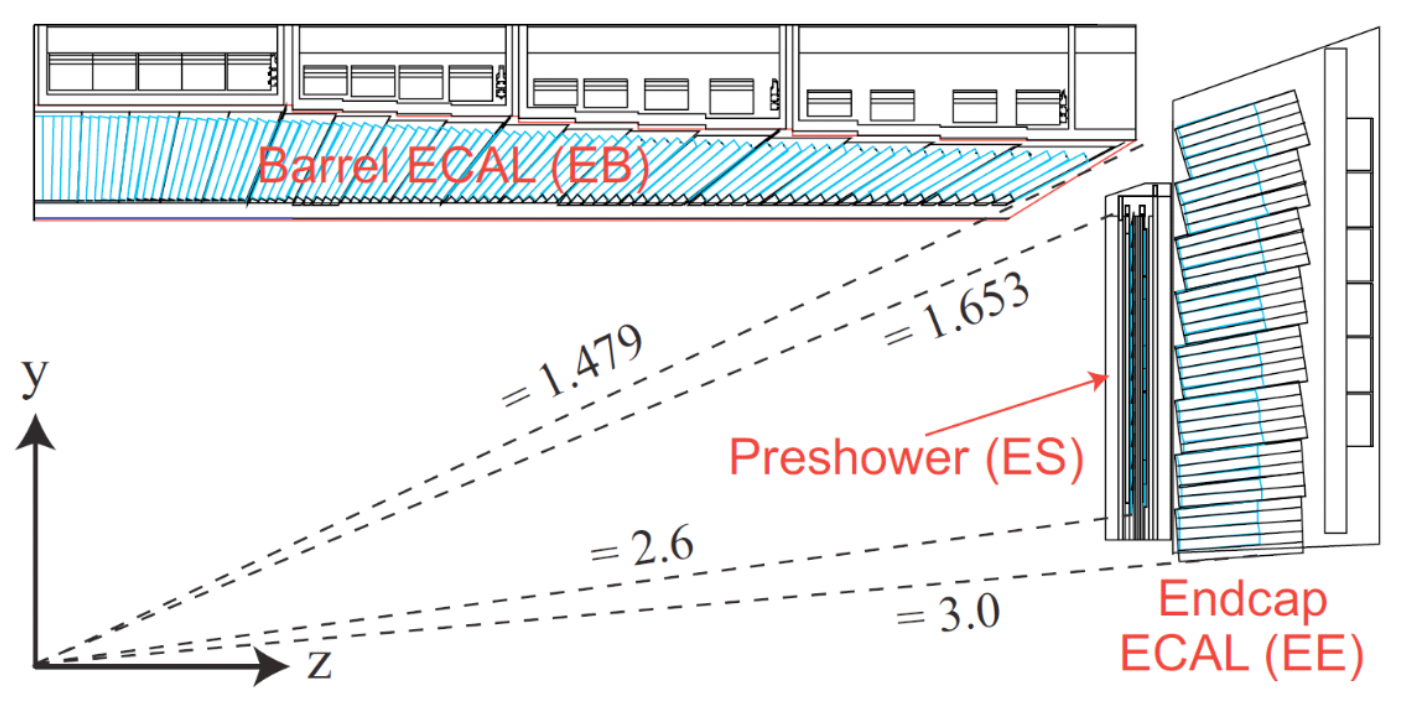
\includegraphics[scale=0.28]{Chapitre3/Images/ECAL.png} 
\caption{Quart de coupe dans le plan $r$-$z$ du calorimètre électromagnétique de CMS \cite{ECAL}.}
\label{ecal}
\end{figure}

\subsubsection{\ding{95} Calorimètre électromagnétique (ECAL)}

Le calorimètre électromagnétique de CMS est un calorimètre homogène dont les modules sont entièrement composés de cristaux de stolzite (\chemform{PbWO_4}) et ans lequel l'énergie des électorns et des photons est mesurée. Ce cristal possède l'avantage d'une bonne résistance aux radiations, d'une courte longueur de radiation $X_0=0,89$ cm correspondant à la distance après laquelle l'énergie d'un électron incident est réduite d'un facteur $1/e$, d'un faible rayon de Molière de $2,2$ cm défini comme le rayon d'un cylindre contenant $90\%$ de l'énergie d'une gerbe et d'un temps de réponse de seulement $15$ ns. L'ECAL constitue la couche de détection suivant le trajectographe et contient deux parties principales : un tonneau cylindrique (EB, \textit{ECAL Barrel)}) couvrant la région définie par $|\eta|<1,479$ et deux bouchons (EE, \textit{ECAL Endcaps}) couvrant la région définie par $1,479<|\eta|<2,6$ (Fig. \ref{ecal}). Le tonneau et les bouchons se composent d'un total de $68~524$ cristaux, dont $61~200$ d'une longueur de $25,8X_0$ dans le tonneau et $7~324$ d'une longueur de $24,7X_0$ dans les bouchons avec chacun une résolution $\Delta\phi\times\Delta\eta=0,0175\times0,0175$. Ces dimensions permettent à chaque cristaux de contenir l'intégralité d'une gerbe électromagnétique produite par une particule incidente et de fournir une estimation de sa direction de vol. Les parties avants du calorimètre sont également équipées d'un système de \textit{preshowering} (ES) placés avant les bouchons dont la granularité élevée permet de différencier un photon seul de deux photons issus de la désintégration d'un pion neutre lorsque ce dernier est fortement boosté. La résolution en énergie $\sigma_E$ du ECAL a été mesurée dans les données à $7$ TeV \cite{ECALres} comme étant :

\begin{equation}
    \frac{\sigma_E}{E}=\frac{0.027}{\sqrt{E}}+\frac{0.12}{E}+0.005,
\end{equation}

avec $E$ l'énergie mesurée et où le premier terme est un terme stochastique issu des fluctuations statistiques de l'énergie des gerbes électromagnétiques, le second est relié au bruit et à l'empilement et le troisième est un terme tenant compte des imperfections du détecteur et des fuites d'énergie.

\begin{figure}
\centering
    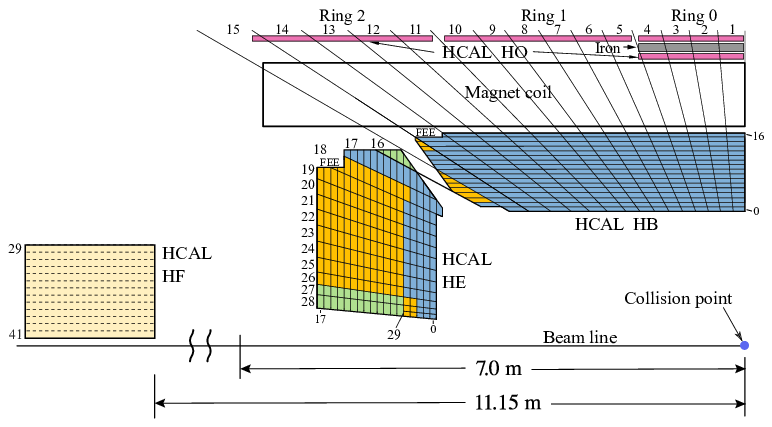
\includegraphics[scale=0.5]{Chapitre3/Images/HCAL.png} 
\caption{Quart de coupe dans le plan $r$-$z$ du calorimètre hadronique de CMS \cite{HCAL}.}
\label{hcal}
\end{figure}

\subsubsection{\ding{95} Calorimètre hadronique (HCAL)}

Le calorimètre hadronique de CMS est un calorimètre inhomogène constitué de couches successives de matériau absorbant dans lequel se forment les cascades et de matériau scintillant. La partie principale du HCAL se situe immédiatement après le ECAL et contient un tonneau (HB, \textit{HCAL Barrel}) couvrant la région $|\eta|<1,4$ et deux bouchons (HE, \textit{HCAL Endcaps}) couvrants la région $1,3<|\eta|<3$ (Fig. \ref{hcal}). Le tonneau et les parties avants contiennent chacune $2~304$ modules d'une résolution $\Delta\phi\times\Delta\eta=0,087\times0,087$ constitués de couches successives de laiton et de plastique scintillant. Une seconde partie du HCAL est également située à l'extérieur de l'aimant pour les particules les plus énergétiques avec une partie centrale (HO, \textit{Outter HCAL}) dans la région $|\eta|<1,3$ et de deux parties avants (HF, \textit{Forward HCAL}) dans la région $2,9<|\eta|<5,2$ (Fig. \ref{hcal}). Tandis que le HO utilise également un plastique scintillant comme matériau actif, le HF requiert une meilleure résistance aux radiations et utilise un matériau constitué de fibres de quartz. Pour ces deux parties externes la culasse en fer de l'aimant joue le rôle d'absorbeur. La résolution en énergie $\sigma_E$ en fonction de l'énergie mesurée $E$ des parties constituées de plastique scintillant est donnée par :

\begin{equation}
    \frac{\sigma_E}{E}=\frac{0,9}{\sqrt{E}}+0.045,
\end{equation}

tandis que celle du HF seul est donnée par :

\begin{equation}
    \frac{\sigma_E}{E}=\frac{1,72}{\sqrt{E}}+0.09.
\end{equation}

\subsection{Chambres à muons}

Les muons interagissent peu avec la matière et possèdent un temps de vol suffisamment long pour s'échapper du détecteur. Les chambres à muons constituent ainsi les dernières couches de détection de CMS placées après l'aimant supraconducteur et sont soumises à un champ magnétique de $1,8$ T grâce à la culasse de retour en fer de ce dernier. Elles sont composées de détecteurs gazeux dont l'ionisation par les muons incidents permet la reconstruction de leur trace et de leur impulsion en combinant les informations du trajectographe en silicium central. 

\begin{figure}
\centering
    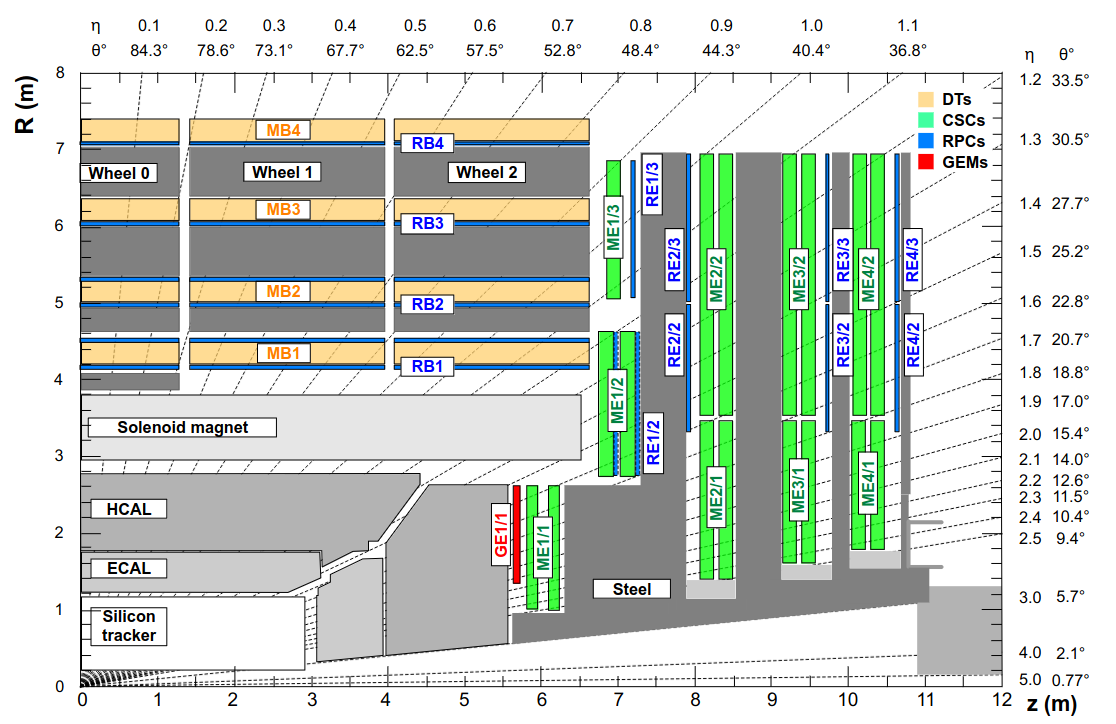
\includegraphics[scale=0.37]{Chapitre3/Images/MUONS.png} 
\caption{Quart de coupe dans le plan $r$-$z$ du système de chambres à muons de CMS \cite{MUONS}.}
\label{muons}
\end{figure}

\subsubsection{\ding{95} Tubes à dérive (DT)}

Les tubes à dérive couvrent la région centrale du détecteur lorsque $|\eta|<1,2$. Chaque élément consiste en un tube creux de section rectangulaire d'environ $1,3\times4,2$ cm$^2$ et rempli de gaz ($85\%$ \chemform{Ar}, $15\%$ \chemform{CO_2}) dans lequel un fil métallique est tendu. Lorsqu'une particule chargée traverse ce volume, elle ionise le gaz présent et l'application d'un champ électrique permet la dérive et la collecte des charges produites sur le fil central qui après amplification génèrent un signal électrique mesurable. La mesure du temps de dérive des électrons au sein du tube permet également de reconstruire une information $2D$ du passage de la particule. Dans CMS, plusieurs de ces tubes sont répartis en couches empilées et quatre couches forment une "super-couche" (\textit{superlayer}). Ces \textit{superlayers} contiennent chacune jusqu'à $90$ tubes et sont elles-mêmes placées par $3$ dans des chambres dont la dimension varie de $2\times2,5$ m$^2$ à $4\times2,5$ m$^2$. Une mesure $3D$ de la trace est obtenue en combinant les informations des différentes \textit{superlayers} au sein d'une chambre : la couche centrale mesure la coordonnée parallèle à l'axe du faisceau et les deux couches externes la coordonnée perpendiculaire avec une résolution spatiale de $100$ $\mu$m.

\subsubsection{\ding{95} Chambres à fils cathodiques (CSC)}

Les chambres à fils cathodiques se situent dans les parties avants de CMS et couvrent la région $0,9<|\eta|<2,4$. Ces dernières sont plus adaptées pour une forte exposition aux radiations et sont constituées, à l'image des chambres à fils, d'anodes filaires croisées à des pistes cathodiques dans un volume de gaz ($40\%$ \chemform{Ar}, $50\%$ \chemform{CO_2}, $10\%$ \chemform{CF_4}).

\subsubsection{\ding{95} Chambres à plaques résistives (RPC)}

Les RPC sont constituées de deux plaques de bakélite séparées par un volume fin de quelques millimètres d'épaisseur et rempli de gaz. Un champ électrique est appliqué entre les deux plaques de forte résistivité, et les charges produites par ionisation lors du passage d'une particule chargée sont collectées par des bandes métalliques externes. Ce système de détection possède une résolution spatiale moindre mais un temps de réponse particulièrement court inférieur à $25$ ns. Les RPC sont ainsi utilisées en complément des CSC et des DT dans le système de déclenchement du détecteur. \\

Un nouveau type de détecteur gazeux appelé \textit{Gas Electron Mutiliplier} (GEM) est également venu récemment compléter le système de chambres à muons de CMS \cite{GEM1,GEM2}. Les GEMs ont pour but d'améliorer la détection des muons dans les parties avants du détecteur en couvrant la région $1,6<|\eta|<2,2$ en prévision de l'augmentation de l'empilement et de l'exposition aux radiations. Un total de $144$ modules ont été installés avant le lancement du Run 3 dans le premier disque de chaque bouchons de CMS et les deux disques suivants seront à leur tour équipés lors du lancement de la phase à haute luminosité. 

\subsection{Système de déclenchement}

Depuis le début du Run 2, le LHC délivre des collisions avec un croisement de paquets de protons toutes les $25$ ns. Ces collisions produisent jusqu'à $40$ millions d'évènements par seconde dont la plupart ont peu d'intérêt physique. Le système de déclenchement de CMS permet de filtrer ces évènements en conservant ceux répondant aux critères jugés intéressants pour les interactions à étudier et ainsi de réduire la quantité de données à stocker. Ce système de déclenchement, aussi désigné par \textit{trigger}, contient un premier niveau L$1$ (\textit{Level 1 Trigger}) et un second niveau HLT (\textit{High Level Trigger}). \\

Le niveau L$1$ est un système de déclenchement purement électronique qui s'appuie sur les informations délivrées par les calorimètres et les chambres à muons sans reconstruction de traces. Les conditions selon lesquelles un évènement est conservé ou non peuvent inclure des limites cinématiques ou requérir la présence de certains objets et sont regroupées au nombre de 256 au sein d'un "menu" sous le nom de \textit{L1 seeds}. Pour chaque évènement, seulement 3,4 $\mu$s sont nécessaires à la prise de décision de l'électronique et le niveau L$1$ permet de réduire la fréquence des événements de $40$ MHz à environ $100$ kHz. \\

Le niveau $HLT$ traite ensuite par un algorithme les évènements conservés par le niveau $L1$ en effectuant une reconstruction rapide de l'évènement et en associant les dépôts d'énergie des calorimètres à des traces grâce aux informations du trajectographe en silicium central. Les critères de sélection du niveau $HLT$ regroupés sous forme de \textit{chemins} permettent de réduire la fréquence des évènements à $1$ kHz et ces derniers sont stockés. \\
    %\chapter{Reconstruction et identification des particules et objets}
\label{chap5}

Ce chapitre est consacré à la description des différentes méthodes de reconstruction et d'identification des particules et objets avec le détecteur CMS. Malgré la grande variété de particules produites lors des collisions proton-proton, seules quelques-unes sont stables à l'échelle du détecteur et peuvent être identifiées. Parmi celles-ci se trouvent les muons ($\mu^{\pm}$), les électrons (e$^{\pm}$), les hadrons chargés (p, $\pi^{\pm}$) et neutres (n, $\pi^0$), et les photons ($\gamma$). Chacune d'elles possède une signature qui lui est propre au sein de chaque sous-détecteur (fig. \ref{CMSslice}) et la combinaison de ces informations à travers l'algorithme du flux de particules, dont une présentation est donnée dans la première partie de ce chapitre, permet leur reconstruction.
Ces particules sont ensuite utilisées comme éléments de base pour la reconstruction d'autres particules ou d'objets plus complexes. Dans la suite, une présentation des méthodes permettant la reconstruction et l'identification des gerbes hadroniques (\textit{jets}) et de l'énergie transverse manquante sera donnée, ainsi qu'une partie dédiée au lepton tau, ce dernier étant l'objet clef de l'analyse réalisée dans cette thèse. 

\section{Algorithme du flux de particules (\textit{Particle Flow})}
\label{PF}

L'algorithme du flux de particules \cite{ThePFAlgo} se fonde sur la combinaison des informations de plusieurs sous-détecteurs pour identifier et reconstruire les particules produites lors des collisions. Le détecteur utilisant l'algorithme doit posséder au moins deux caractéristiques essentielles pour un fonctionnement optimal. La première repose sur un champ magnétique suffisamment fort ainsi qu'une bonne granularité des calorimètres afin d'éviter le recouvrement des dépôts d'énergie et assurer une bonne séparation entre hadrons neutres et chargés. La seconde repose sur la bonne performance du trajectographe et sur un faible budget de matière pour ne pas altérer la mesure des calorimètres. Dans le cas de CMS, ces aspects sont couverts par son trajectographe en silicium équipé de pixels et de bandes, l'excellente granularité de son calorimètre électromagnétique et la bonne hermicité de son calorimètre hadronique. L'aimant supraconducteur est placé à l'extérieur de ces éléments, ce qui permet une meilleure association entre les informations du trajectographe et des calorimètres. Enfin, les larges dernières couches de détection dédiées aux muons permettent une reconstruction et une identification optimale de ces derniers en complétant les informations du trajectographe. \\

\begin{figure}
\centering
    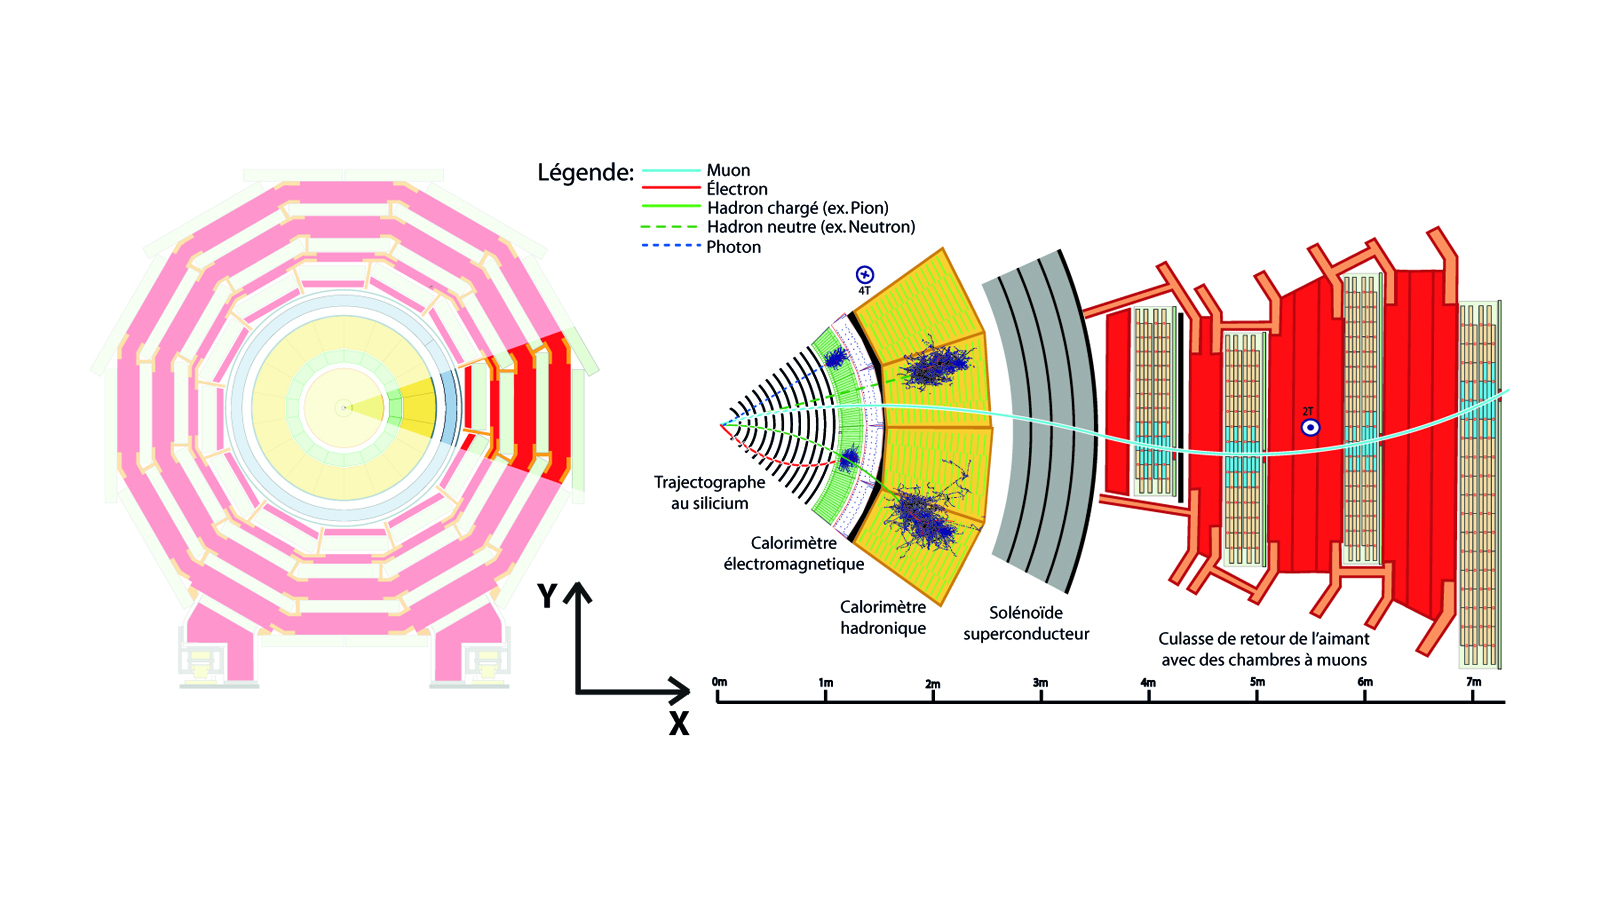
\includegraphics[scale=1.1]{Chapitre4/Images/CMSslice.png} 
    \caption{Vue en tranche d'une section de CMS et signature caractéristique de chaque particule. Les particules chargées sont déviées par le champ magnétique et déposent une trace dans le trajectographe. Électrons et photons sont stoppés les premiers par le calorimètre électromagnétiques. Les hadrons sont stoppés par la calorimètre hadronique. Les muons traversent l'intégralité du détecteur et leur trace dans le trajectographe est complétée dans les chambres à muons \cite{Barney:2120661}.}
    \label{CMSslice}
\end{figure} 

Pour un évènement donné, l'algorithme utilise deux types de réponses du détecteur comme point de départ de la reconstruction : les impacts (\textit{hits}) associés aux particules chargées dans les couches du trajectographe et des chambres à muons ainsi que les dépôts d'énergie dans les calorimètres regroupés en amas (\textit{clusters}). Les premiers sont utilisés afin de reconstruire des traces associées à la trajectoire des particules à partir d'une méthode combinatoire nommée \textit{"Combinatorial Track Finder"} (CTF) \cite{Elmetenawee:2020emw} s'appuyant sur l'application de filtres de Kalman avec une minimisation de l'erreur par des tests de $\chi^2$. Le processus peut se résumer en quatre étapes :

\begin{enumerate}
    \item \textbf{\textit{Seeding}} : formation de \textit{seeds} constituées de triplets ou de quadruplets de \textit{hits} compatibles avec une trace et dont le seuil en impulsion transverse dépasse un minimum requis.
    \item \textbf{\textit{Building}} : Extrapolation de la trace construite a partir des \textit{seeds}. À chaque couche du trajectographe, la compatibilité de chaque \textit{hit} candidat à la formation de la trace est testée grâce aux filtres de Kalman par un test de $\chi^2$ et ceux dont la valeur est minimale sont choisis.
    \item \textbf{\textit{Fitting}} : les traces ainsi formées sont ajustées et les 5 paramètres de la trace hélicoïdale sont déterminés. 
    \item \textbf{\textit{Selection}} : un marqueur de qualité de reconstruction de la trace lui est attribué et celles de qualité moindre sont écartées. 
\end{enumerate}

Cette méthode de reconstruction de traces itérative (\textit{Iterative Tracking}) \cite{IterativeTracking} répète ces étapes jusqu'à 12 fois en retirant les impacts déjà associés à une trace à chaque itération, simplifiant ainsi le processus combinatoire. La figure \ref{etatrackefficiency} présente l'efficacité de reconstruction d'une trace dans un échantillon d'événements $t\overline{t}$ simulés en fonction de sa coordonnée $\eta$, ainsi que la probabilité de reconstruire une trace qui n'est en réalité pas associée à une particule. Une comparaison des performances de CMS entre 2016 et 2017 avant et après l'ajout d'une nouvelle couche de pixels au sein du trajectographe est également montrée, avec une amélioration globale dans les parties avant du détecteur. La figure \ref{pttrackefficiency} présente quant à elle l'efficacité globale de reconstruction dans le même échantillon en fonction de l'impulsion transverse de la trace ainsi que la contribution de diverses sous-parties du trajectographe et du type de \textit{seed} à l'origine de la trace. La perte d'efficacité observée aux extrema dans la même figure s'explique principalement par un effet d'enroulement de la trajectoire sous la contrainte du champ magnétique pour les traces à basse impulsion, et par une faible courbure pour celles à haute impulsion les rendant plus difficilement identifiables. \\

\begin{figure}
  \begin{subfigure}{0.5\linewidth}
    \centering
    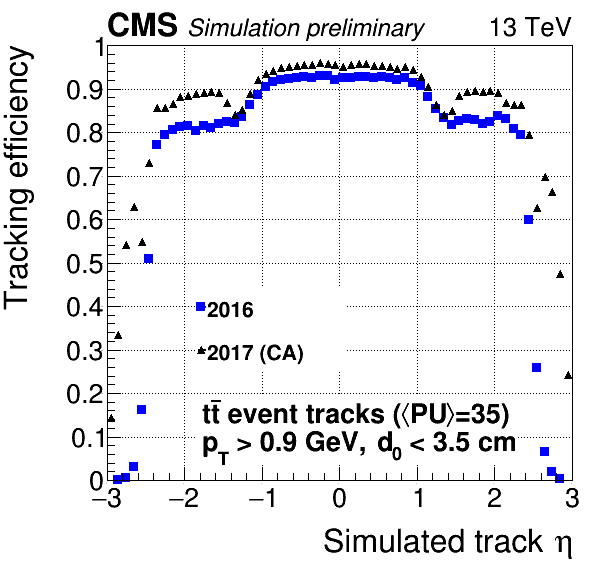
\includegraphics[width=0.95\linewidth]{Chapitre4/Images/efficiency_eta_1.png} 
    \caption*{} 
  \end{subfigure}
  \begin{subfigure}{0.5\linewidth}
    \centering
    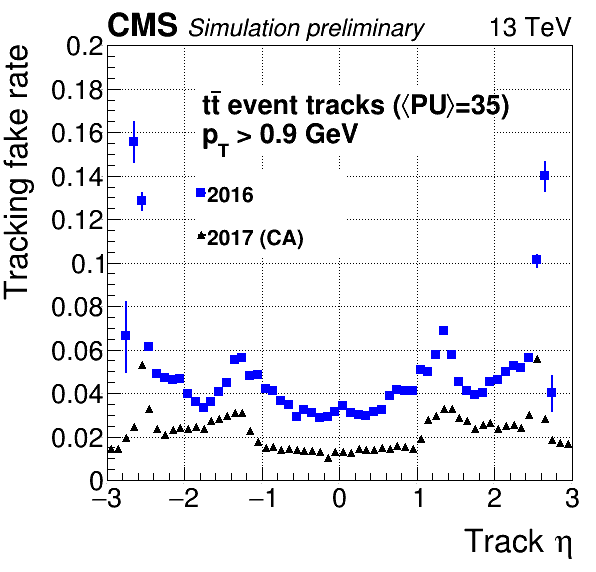
\includegraphics[width=0.95\linewidth]{Chapitre4/Images/fake_eta_1.png} 
    \caption*{} 
  \end{subfigure} 
  \caption{Efficacité de reconstruction (gauche) et taux de faux (droite) pour des traces reconstruites dans des échantillons $t\overline{t}$ simulés en fonction de la coordonnées $\eta$. Les performances avant (bleu) et après (noir) l'ajout de pixels au sein du trajectographe sont également comparées \cite{Elmetenawee:2020emw}.}
  \label{etatrackefficiency}
\end{figure}

Dans le cas des calorimètres, un algorithme de regroupement (\textit{clustering algorithm}) est utilisé afin de collecter les dépôts d'énergie et former des amas. Cet algorithme a notamment pour but de mesurer l'énergie et la direction des particules neutres dans le calorimètre électromagnétique en les isolant des particules chargées, ainsi que de regrouper les photons issus du rayonnement de freinage des électrons. Dans un premier temps l'algorithme identifie les maxima locaux d'énergie au-delà d'un certain seuil puis les associe aux cellules voisines dont l'énergie est au moins deux fois significativement supérieure au bruit (de $80$ MeV à $300$ MeV dans l'ECAL et jusqu'à 800 MeV dans le HCAL) pour former des amas dits "topologiques". \\

\begin{figure}[!ht]
\centering
    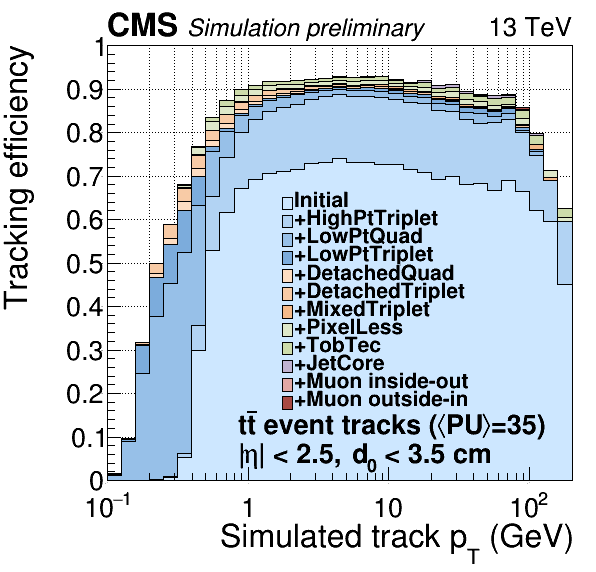
\includegraphics[width=0.6\linewidth]{Chapitre4/Images/MC_eff.png} 
    \caption{Efficacité de reconstruction pour des traces reconstruites dans des échantillons $t\overline{t}$ simulés en fonction de l'impulsion transverse. Les performances dans différentes sous parties du détecteurs et pour différents types de \textit{seed} initiale sont également présentées \cite{Elmetenawee:2020emw}.}
    \label{pttrackefficiency}
\end{figure} 

Enfin, un algorithme de raccordement (\textit{link algorithm}) est utilisé afin d'établir un lien entre traces et amas, ainsi qu'entre amas des différents calorimètres. Les traces sont d'abord propagées aux calorimètres couche par couche depuis la position de leur dernier impact dans le trajectographe, puis sont associées à un amas donné si la position de la trace et celle de l'amas coïncident dans le plan $\eta$-$\phi$. Deux amas sont ensuite associés si l'amas du calorimètre électromagnétique est englobé dans celui du calorimètre hadronique dans le plan $\eta$-$\phi$. Une procédure similaire est appliquée dans les parties avant du détecteur en considérant en plus les amas du système de \textit{preshowering} du ECAL en englobant l'amas du calorimètre le plus granulaire dans celui du moins granulaire. Finalement les éléments entre lesquels l'algorithme a établi un lien direct ou indirect sont regroupés pour former des "blocs".

\subsection{Muons}
\label{MuonID}

Les muons sont les candidats les plus facilement identifiables, notamment grâce à leur capacité à traverser l'intégralité des couches du détecteur, et sont donc traités en premier par l'algorithme du flux de particules \cite{Sirunyan:2313130}. Une trace reconstruite dans le trajectographe par l'algorithme CTF sera associée à un muon (\textit{tracker muon}) dans le cas où cette dernière possède une impulsion totale supérieure à $2,5$ GeV pour une composante transverse d'au moins $0,5$ GeV et si elle coïncide avec au moins un segment des chambres à muons. La correspondance entre segment et trace est vérifiée si leur distance selon l'axe $x$ est inférieure à $3$ cm ou si le quotient de cette distance par son erreur est inférieur à 4. D'autre part une trace peut être reconstruite de manière isolée dans les chambres à muons (\textit{stand-alone muon}) par combinaison des informations des différents sous-détecteurs de ces dernières par application de filtres de Kalman. Enfin un muon dit "global" (\textit{global muon}) est reconstruit par propagation de la trace d'un \textit{stand-alone muon} à celle d'un \textit{tracker muon} si ces deux traces sont compatibles à travers un ajustement combiné et en choisissant l'association dont l'erreur est minimale si plusieurs candidats existent. Environ $99$\% des muons contenus dans l'acceptance géométrique du détecteur sont ainsi reconstruits dans le trajectographe et le plus souvent de manière globale. Les muons reconstruits par le trajectographe seul possèdent une meilleure efficacité de reconstruction dans les zones du détecteur à faible instrumentation et pour les muons à basse impulsion transverse. Ils souffrent toutefois d'une plus haute probabilité d'erreur d'identification, notamment en raison de certaines gerbes hadroniques de haute impulsion capables d'atteindre les premiers segments des chambres à muons. Les traces reconstruites dans les chambres à muons uniquement sont quant à elles sujettes à une plus grande contamination par les muons cosmiques et possèdent une plus faible résolution sur l'impulsion. La combinaison des informations du trajectographe et des chambres à muons permet alors de diminuer le taux de faux muons et d'améliorer la résolution sur leur impulsion, en particulier pour une impulsion transverse supérieure à $200$ GeV. La figure \ref{dimuon} présente une distribution de la masse invariante des paires de muons reconstruites par le détecteur CMS. L'excellente résolution permet notamment d'observer les résonances les plus connues issues de la désintégration de mésons ou du boson $Z$. \\

\begin{figure}
\centering
    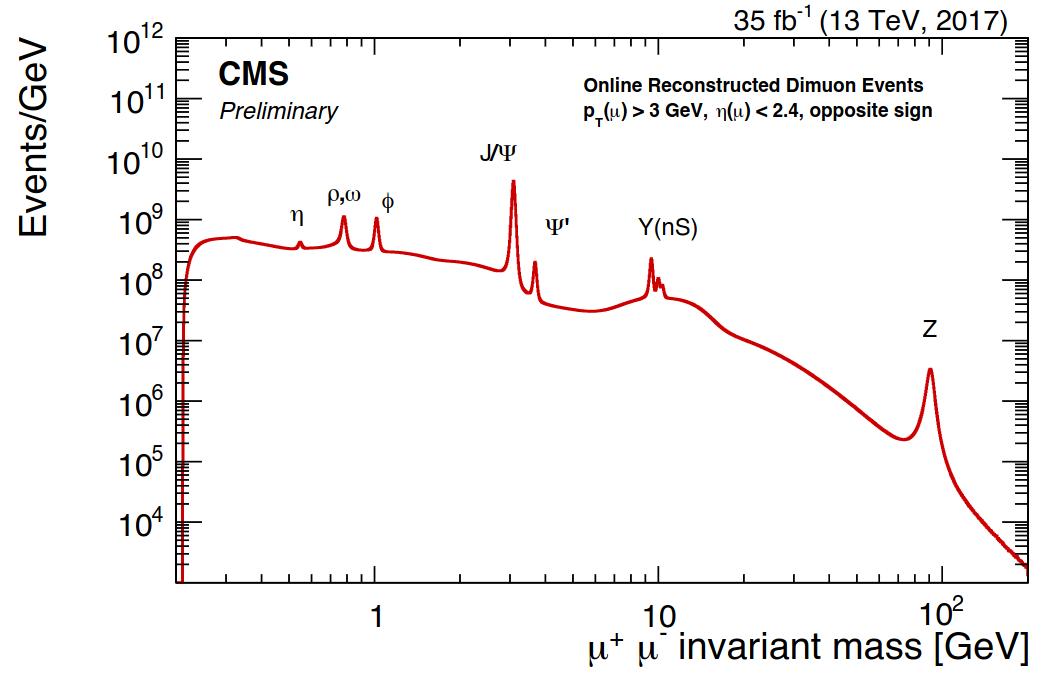
\includegraphics[width=0.8\linewidth]{Chapitre4/Images/dimuon.png} 
    \caption{Masse invariante des paires de muons $\mu^+\mu^-$ sélectionnées par le système de déclenchement et reconstruites par le détecteur CMS dans les données 2017 \cite{Dimuon}.}
    \label{dimuon}
\end{figure} 

Par la suite, une série de variables destinées à caractériser les muons reconstruits est mise en place afin de permettre d'effectuer une sélection basée sur un équilibre entre pureté et efficacité. Ces dernières reposent notamment sur le nombres d'impacts de la trace, le nombre de segments associés ou encore la qualité de l'ajustement. D'autres peuvent également servir à différencier un muon issu du vertex primaire (\textit{prompt muon}) comme dans le cas d'une désintégration $Z\rightarrow\mu^+\mu^-$ de ceux issus d'un vertex secondaire produits en particulier dans des désintégrations de bosons $W^{\pm}$ en association à des jets. C'est notamment le cas de la variable relative d'isolement qui est définie comme le quotient de la somme de l'énergie des particules dans un cône $\Delta R=\sqrt{(\Delta\phi)^2+(\Delta\eta)^2}$ autour du muon et de son impulsion transverse.

\subsection{Électrons et photons isolés}
\label{EGammaID}

Plusieurs phénomènes d'interaction rayonnement-matière font de l'identification des électrons et des photons deux processus complémentaires et indissociables. D'une part, les électrons sont sujets à la perte d'une fraction de leur énergie par rayonnement de freinage au sein du trajectographe sous formes de photons. D'autre part, les photons sont susceptibles de créer des paires e$^+$/e$^-$. Dans les deux cas, électrons et photons vont de manière générale venir déposer leur énergie au sein de calorimètre électromagnétique non plus sous la forme d'une seule particule mais sous celle d'une gerbe électromagnétique. Leur reconstruction et identification est entièrement intégrée dans l'algorithme du flux de particules et s'appuie sur les traces et amas dont la construction est décrite au début de ce chapitre. Dans un premier temps, plusieurs amas du calorimètre électromagnétique sont regroupés en "superamas" (SC, \textit{superclusters}) dans une région spécifique autour d'un amas choisi comme étant celui avec un maximum d'énergie et une énergie transverse supérieure à $1$ GeV. Cette procédure vise à regrouper les différentes particules d'une gerbe électromagnétique au sein d'un seul amas centré sur le dépôt d'énergie principal. Les traces du trajectrographe compatibles avec un SC servent ensuite de point de départ à l'algorithme GSF (\textit{Gaussian Sum-Filter}) \cite{Adam_2005} dont le but est de reconstruire la trace des électrons en modélisant l'énergie perdue sous forme de photons par une somme pondérée de distributions gaussiennes. En parallèle, la compatibilité du reste des traces est testée avec l'hypothèse de la trajectoire d'un électron et sont également injectées dans l'algorithme GSF en cas de succès. Les traces provenant d'une conversion de photon en paire e$^+$/e$^-$ sont quant à elles identifiées grâce à un algorithme dédié en recherchant notamment des vertex déplacés, et permettent de compléter la mesure du calorimètre électromagnétique seul. A ce stade toutes les traces GSF et superamas sont regroupés en blocs de flux de particules et sont encore indifférenciés entre électrons et photons. \\

Enfin, les candidats électrons sont formés à partir des blocs dans lesquels se trouve un superamas associé à au moins une trace GSF et un maximum de deux traces additionnelles. Les candidats photons sont quant à eux formés à partir des blocs dans lesquels un superamas possède une énergie transverse supérieure à $10$ GeV et sans lien établi avec une trace GSF. Les candidats issus de cette sélection forment une première collection d'électrons et de photons utilisée dans la plupart des analyses s'appuyant sur ce type d'objets. 

\subsection{Hadrons et photons non isolés}
\label{HadID}

Les hadrons constituent les derniers éléments reconstruits et identifiés par l'algorithme du flux de particules avant la reconstruction d'objets plus complexes. Ces derniers sont généralement directement reconstruits en tant que hadrons chargés ($\pi^{\pm}, K^{\pm}, p$) ou neutres ($K^0_L, n$), mais peuvent également être reconstruits sous la forme de photons non isolés dans le cas de la désintégration $\pi^0\rightarrow\gamma\gamma$ du pion neutre dont le rapport d'embranchement est de $98,823\pm0.034\%$ \cite{PDG2022}. \\

De manière générale, les photons et les hadrons neutres sont associés à des dépôts d'énergie au sein des calorimètres dont aucun lien n'a été établi avec une trace. Pour les régions du détecteur situées dans l'acceptance du trajectographe ($|\eta|<2.5$), chaque dépôt d'énergie n'ayant pas été associé à une trace dans le calorimètre électromagnétique est associé à un photon tandis qu'un dépôt dans le calorimètre hadronique est associé à un hadron neutre. Cette hypothèse repose sur le principe qu'environ $25\%$ de l'énergie des gerbes hadroniques provient de photons tandis que les hadrons neutres sont responsables de seulement $3\%$ de l'énergie déposée dans le calorimètre électromagnétique. En dehors de cette acceptance, les hadrons chargés et neutres ne sont pas différenciables et entraînent le dépôt de 25$\%$ de l'énergie des jets au sein du calorimètre électromagnétique. Les photons sont alors identifiés dans ces régions lorsqu'un amas dans le calorimètre électromagnétique n'est associé à aucun amas dans le calorimètre hadronique, puis les amas entre lesquels un lien est établi sont associés à des hadrons. Afin d'identifier les éventuels photons et hadrons neutres dont les dépôts d'énergie serait superposés à ceux de hadrons chargés, l'algorithme s'appuie sur une procédure de calibration précise des dépôts d'énergie produits par des particules neutres réalisés en amont des prises de données grâce à des tests sur faisceaux, par exposition à des sources radioactives ou encore par mesure du rayonnement cosmique. \\

Après calibration des photons et hadrons précédemment identifiés, les amas restants dans le calorimètre hadronique sont associés à une ou plusieurs traces du trajectographe, elles-mêmes ensuite associées aux éventuels amas restants dans le calorimètre électromagnétique à raison de une trace par amas. Le contenu exact des blocs ainsi formés est identifié grâce à la somme des impulsions des traces incluses. Dans le cas où la somme des impulsions est supérieure à l'énergie calibrée du bloc avec une différence supérieure à la résolution en énergie des hadrons, la présence de photons et de hadrons neutres est indiquée. Si cette différence se situe entre l'énergie déposée dans le calorimètre électromagnétique seul et une valeur maximale de $500$ MeV, un photon dont l'énergie est égale à la différence mesurée est identifié. Au-delà, un photon dont l'énergie est égale à l'énergie déposée dans le calorimètre électromagnétique seul est identifié et l'énergie restante est attribuée à la présence d'un hadron neutre lorsque celle-ci est supérieure à $1$ GeV. Enfin, chaque trace donne lieu à un hadron chargé dont les propriétés cinématiques sont celles de la trace et dont la masse est fixée à celle d'un pion chargé. Lorsque l'énergie calibrée du bloc est compatible avec la somme des impulsions des traces alors aucun hadron neutre n'est reconstruit. Dans de plus rares cas, l'énergie calibrée peut également être inférieure à la somme des impulsions des traces. Dans ce cas, une recherche de muon est effectuée, ces derniers déposant généralement peu d'énergie au sein des calorimètres. Si un excès est toujours observé, la recherche se porte sur la qualité de reconstruction des traces et une exclusion lorsque l'erreur associée à une trace est supérieure à $1$ GeV.

\section{Jets et énergie transverse manquante (MET)}
\label{JetMetID}

\begin{figure}
\centering
    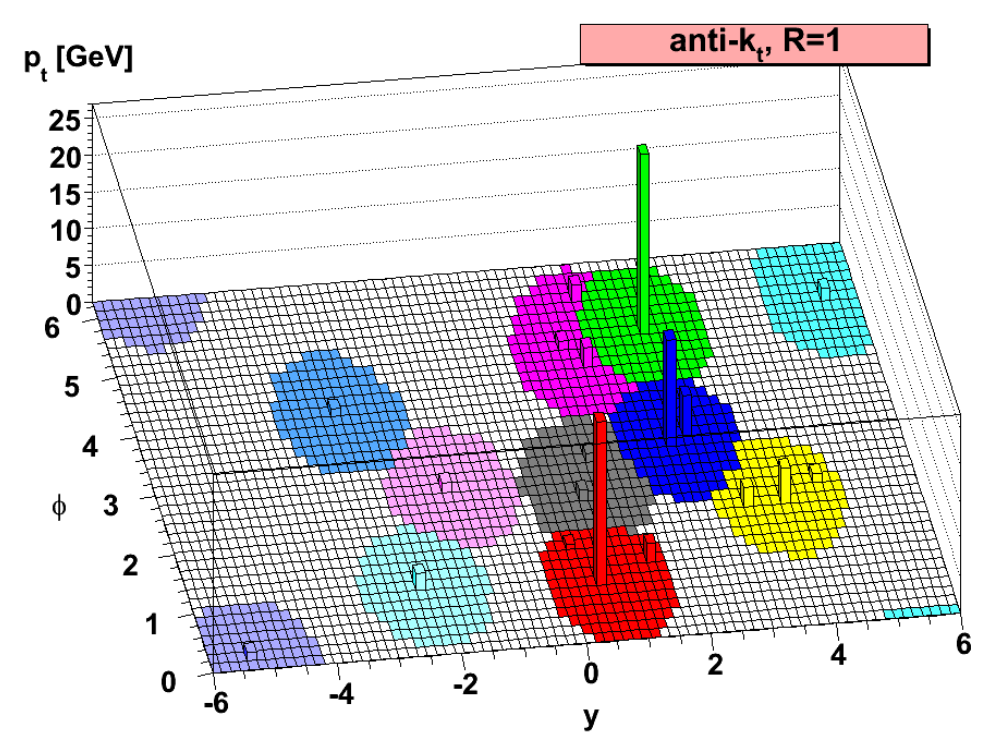
\includegraphics[width=0.6\linewidth]{Chapitre4/Images/antikt.png} 
    \caption{Représentation des jets reconstruits par l'algorithme anti-$k_t$. Chaque couleur représente un \textit{cluster} différent \cite{antikt}.}
    \label{antikt}
\end{figure} 

Une des propriétés fondamentale de la QCD est d'imposer aux quarks un confinement à travers lequel ces derniers ne peuvent exister à l'état libre tel que mentionné dans la section \ref{QCD}. Cette propriété donne lieu à un processus d'hadronisation durant lequel quarks et gluons forment des jets de hadrons au sein du détecteur. L'algorithme du flux de particules permet la reconstruction de ces objets par association des différents éléments reconstruits précédemment en s'appuyant sur un algorithme de regroupement anti-$k_t$ (\textit{anti-$k_t$ jet clustering algorithm}) \cite{antikt}, où $k_t$ désigne l'impulsion transverse ($p_T$) d'un objet. Tout algorithme de regroupement s'appuie sur une définition particulière de la distance entre deux objets ($d_{ij}$) et de celle entre un objet et le faisceau ($d_iB$) en considérant tous les objets à l'intérieur d'un cône de taille donnée. Ces distances s'écrivent :

\begin{align}
    d_{ij} & = \mbox{min}\bigl(k_{ti}^{2p},k_{tj}^{2p}\bigr)\frac{\Delta_{ij}^2}{R^2}, \\
    d_{iB} & = k_{ij}^{2p},
\end{align}

avec $\Delta^2_{ij}=(y_i-y_j)^2+(\phi_i-\phi_j)^2$, et où $k_{ti}$ représente l'impulsion transverse de l'objet $i$, $y_i$ sa rapidité et $\phi_i$ sa coordonnée azimuthale. $R$ représente la taille du cône à l'intérieur duquel l'algorithme opère, fixée à $0,4$ lors du Run 2. La particularité de l'algorithme anti-$k_t$ repose sur la valeur du paramètre $p$ fixée à $-1$, où cette valeur sera positive pour un algorithme classique de type $k_t$. L'algorithme procède ensuite de manière itérative sur tous les hadrons de l'évènement en calculant pour chacun les distances $d_{ij}$ et $d_{iB}$ puis en classant ces distances par ordre décroissant. En commençant par la valeur minimale, si cette distance est de type $d_{ij}$ les impulsions des particules $i$ et $j$ sont sommées. Si la distance est de type $d_{iB}$, la particule $i$ est associée à un jet puis retirée de la liste. L'algorithme répète ensuite cette procédure jusqu'à ce que tous les objets soient associés à un jet. Lorsque qu'un jet est isolé il possède une forme caractéristique conique telle que montrée dans la figure \ref{antikt}, et sa composition typique en énergie est donnée dans la figure \ref{JetEnergy}. \\

\begin{figure}
    \begin{subfigure}{0.5\linewidth}
    \centering
    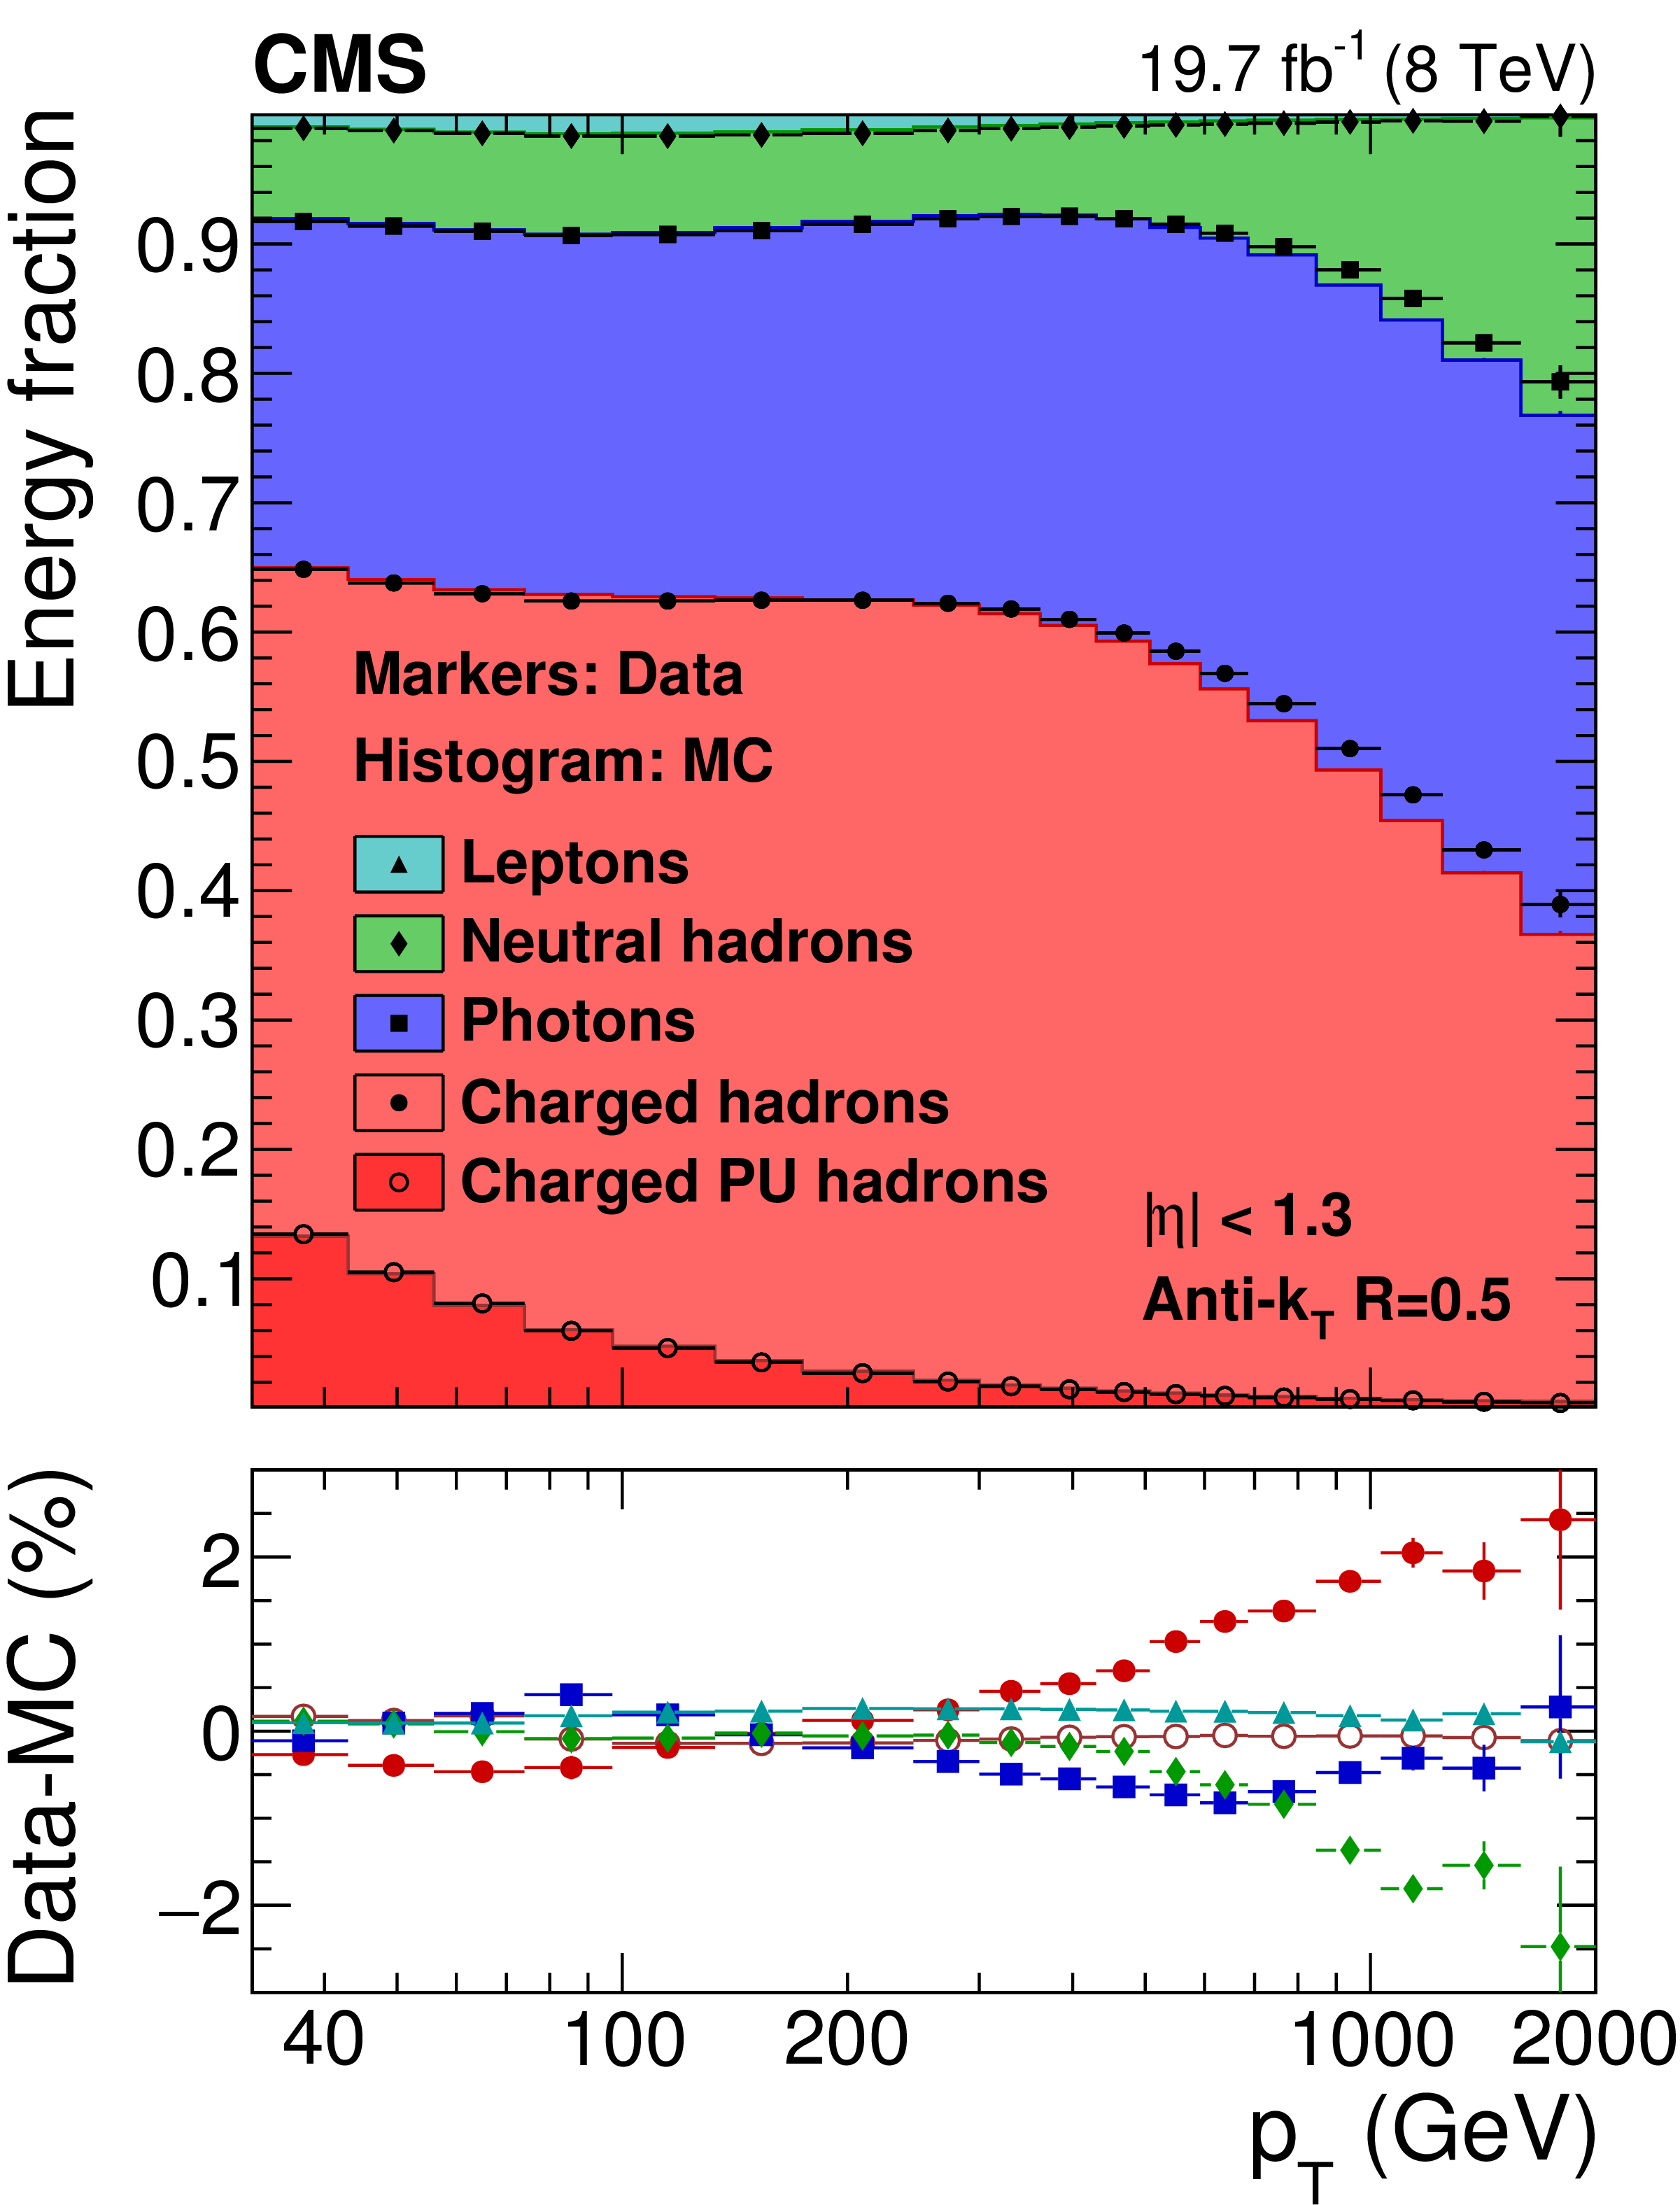
\includegraphics[width=\linewidth]{Chapitre4/Images/PFJetPT.png} 
    \caption*{} 
    \end{subfigure}
    \begin{subfigure}{0.5\linewidth}
    \centering
    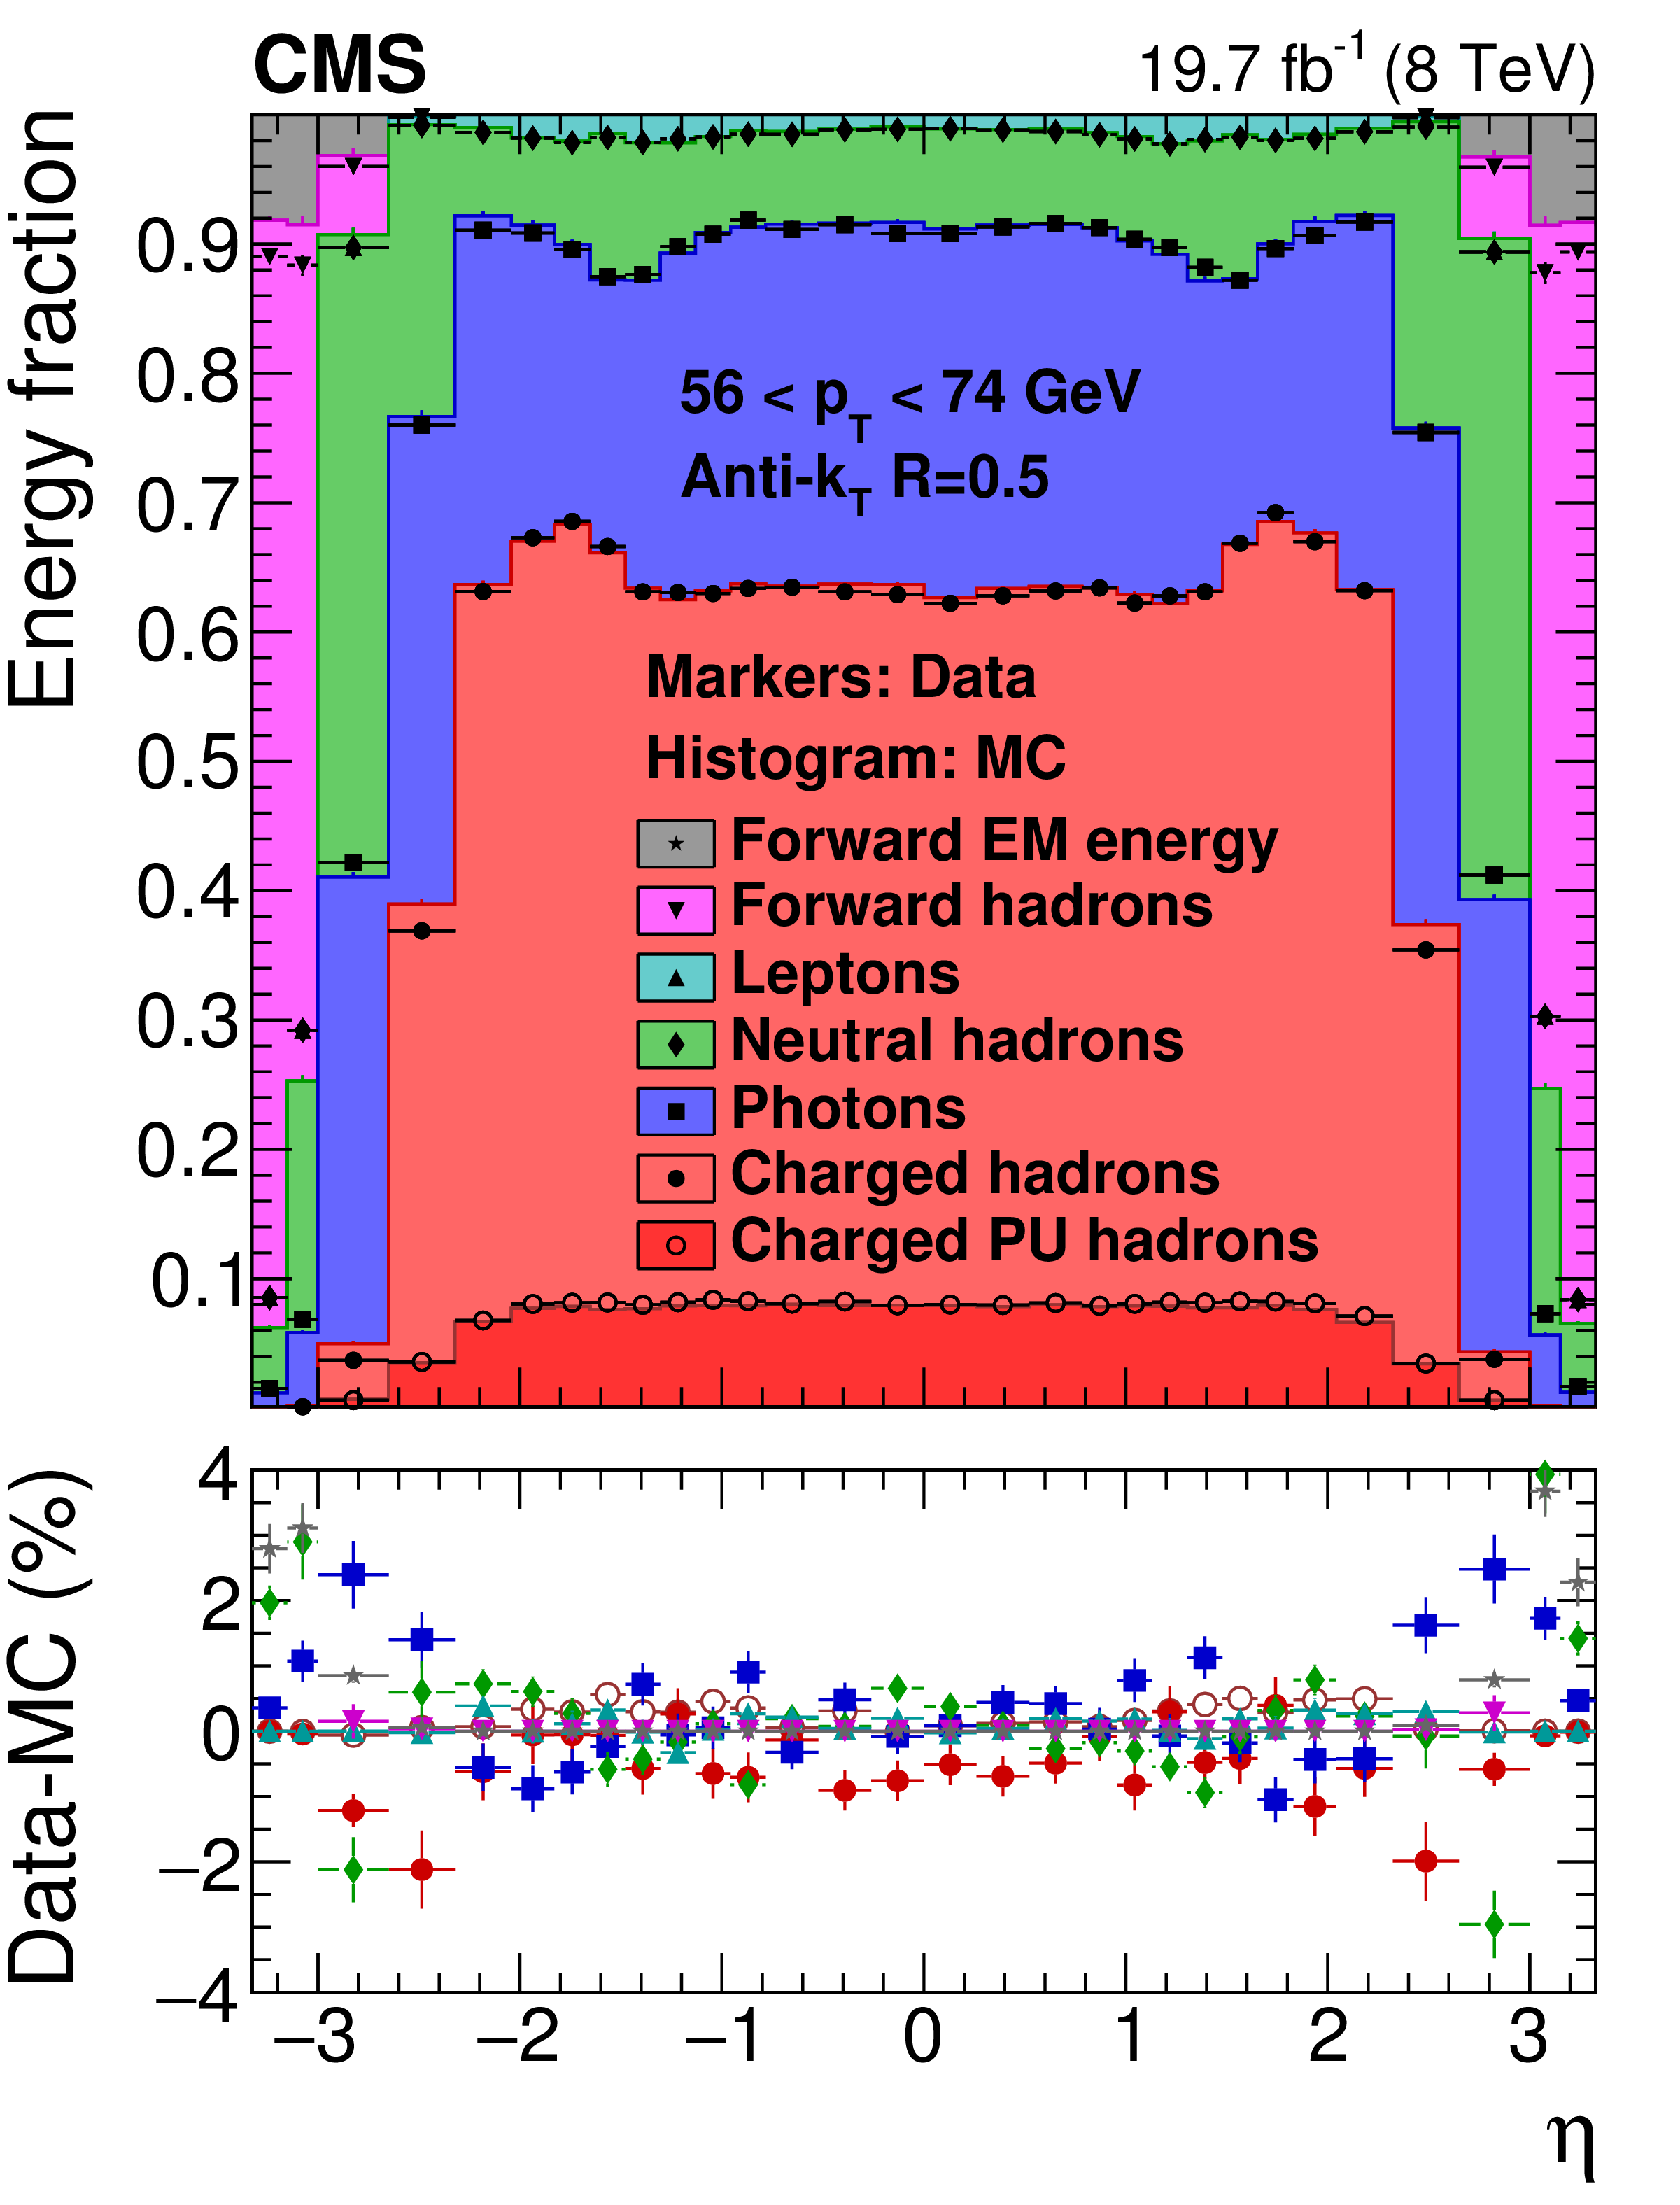
\includegraphics[width=\linewidth]{Chapitre4/Images/PFJetETA.png} 
    \caption*{} 
    \end{subfigure}
    \caption{Composition en énergie des jets et comparaison entre données et simulation en fonction de l'impulsion transverse (gauche) et de la coordonnée $\eta$ (droite). Les hadrons chargés associés à un vertex issu de l'empilement sont dénotés "\textit{Charged PU hadrons}" \cite{ThePFAlgo}.}
    \label{JetEnergy}
\end{figure}

La MET peut être déterminée à partir de l'inverse de la somme des impulsions transverses de tous les objets directement issus de l'algorithme du flux de particules au sein d'un évènement et est alors appelée PF MET. Elle peut également être mesurée à partir des informations des calorimètres seuls (Calo MET). Une comparaison de la résolution entre cette dernière et la PF MET est donnée dans la figure \ref{METreso}. Enfin, l'algorithme PUPPI \cite{puppi} sera également introduit dans la section \ref{MET} pour les besoins de l'analyse présentée dans le chapitre \ref{analysis}.

\begin{figure}
    \centering
    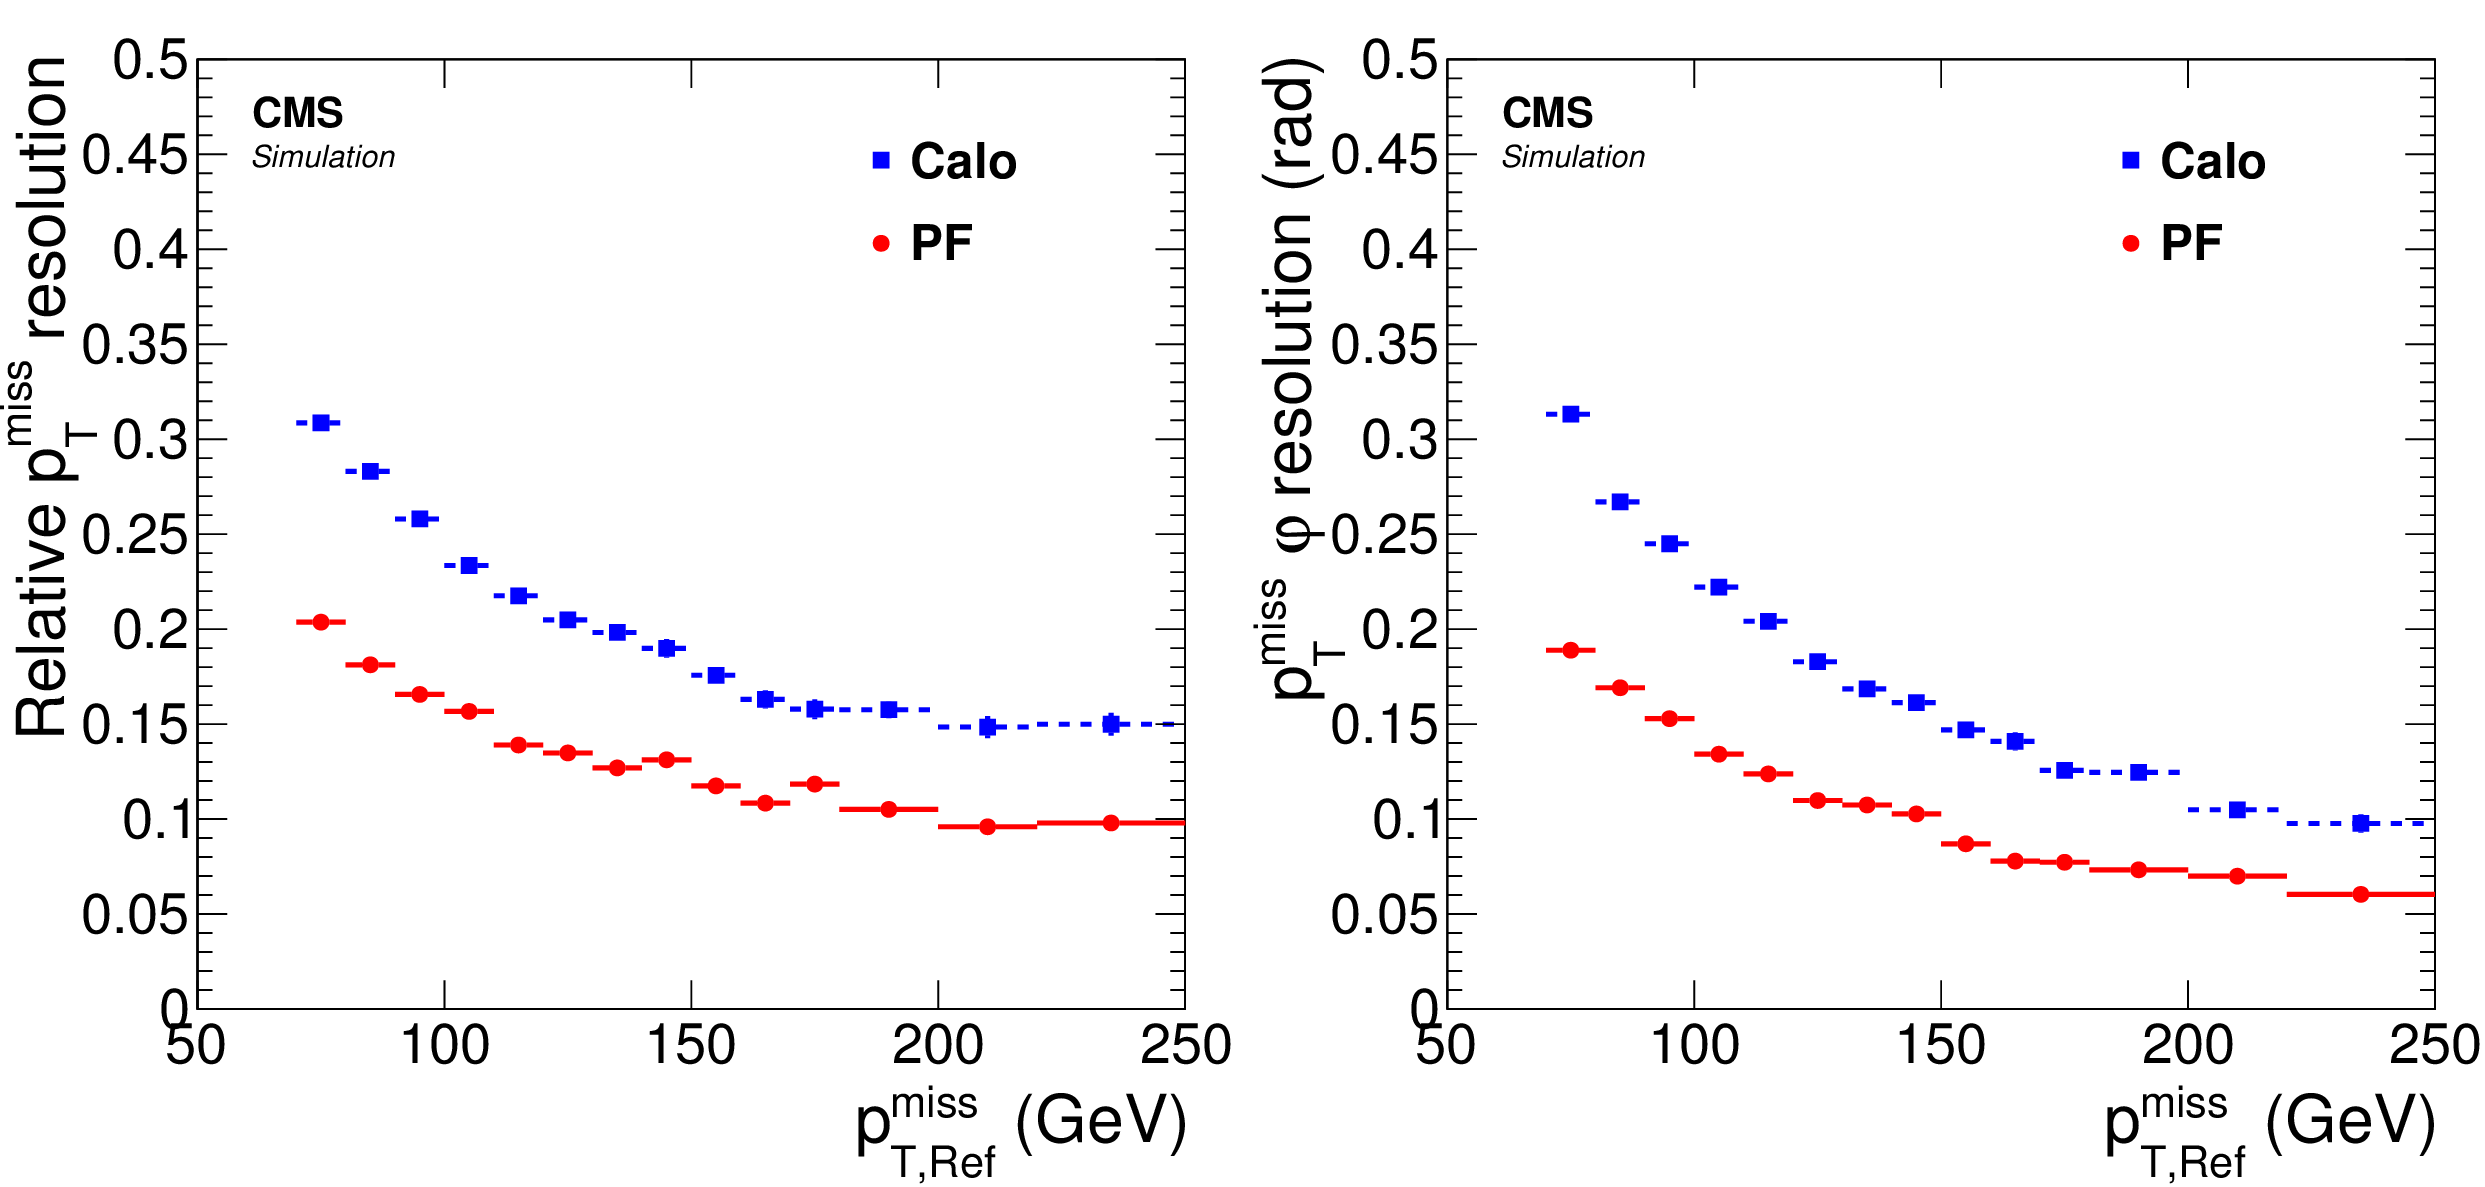
\includegraphics[scale=0.15]{Chapitre4/Images/METres.png}
    \caption{Résolution relative et résolution angulaire de la PF MET et de la Calo MET mesurées dans des échantillons d'événements $t\overline{t}$ simulés \cite{PFalgo}.}
    \label{METreso}
\end{figure}

\section{Leptons tau}

Ce paragraphe vise à introduire les propriétés du lepton tau ainsi que les méthodes de reconstruction et d'identification employées au sein de CMS. D'autres méthodes, propres aux besoins de l'analyse de la structure CP du couplage de Yukawa du lepton tau, seront également présentées dans la section \ref{eventreco} du chapitre \ref{analysis}.

\begin{figure}[b]
\centering
    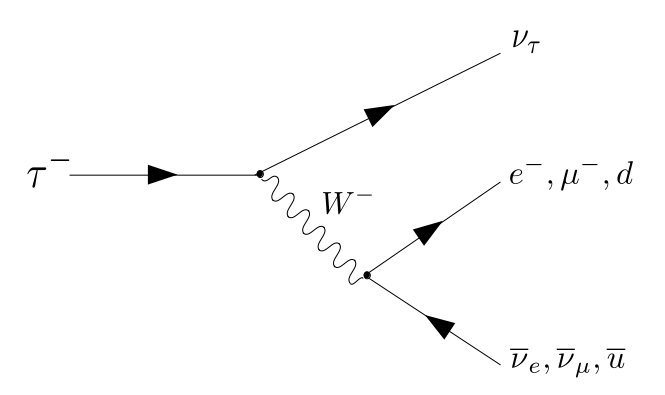
\includegraphics[width=0.6\linewidth]{Chapitre4/Images/taudecay.png} 
    \caption{Diagramme de Feynman associé à la désintégration d'un lepton tau.}
    \label{taudecay}
\end{figure} 

\subsection{Propriétés}
\label{tau properties}
Le lepton tau appartient à la troisième génération des fermions avec une masse $m_{\tau}=1.77$ GeV$\simeq3500~m_e$ faisant de lui une particule hautement instable. Sa désintégration fait intervenir un courant chargé (fig. \ref{taudecay}) à travers lequel un neutrino tau est produit. Le boson W émis produit dans un tiers des cas une désintégration leptonique vers un électron ou un muon accompagné d'un neutrino de même saveur, et une désintégration hadronique à travers une paire de quark dans les deux tiers des cas restants. Les différents états finaux de la désintégration du lepton tau et leur rapport d'embranchement sont présentés dans le tableau \ref{tabDM}. Son temps de vie de l'ordre de $10^{-13}$ secondes lui offre un temps de vol trop court pour atteindre les premières couches de détection du trajectographe de CMS et ainsi seuls ses produits de désintégration, à l'exception des neutrinos, sont détectés. \\

\begin{table}[h]
\centering
\begin{tabular}{|ll|l|ll}
\hline \hline
\multicolumn{2}{c|}{\begin{tabular}[c]{@{}c@{}}Mode de désintégration\\ $\tau^-\rightarrow$\end{tabular}}                                          & \multicolumn{1}{c|}{\begin{tabular}[c]{@{}c@{}}Résonance\\ intermédiaire\end{tabular}} & \multicolumn{2}{c}{BR(\%)}                       \\ \hline \hline
\multicolumn{1}{c|}{\multirow{2}{*}{Leptonique}} & e$^-\overline{\nu}_e\nu_{\tau}$   &                                                                                        & \multicolumn{1}{l|}{17.4} & \multirow{2}{*}{35.2} \\[3pt] \cline{2-4}
\multicolumn{1}{c|}{}                            & $\mu^-\overline{\nu}_e\nu_{\tau}$ &                                                                                        & \multicolumn{1}{l|}{17.8} &                       \\ [3pt] \hline \hline
\multicolumn{1}{l|}{\multirow{6}{*}{Hadronique}} & $\pi^-\nu_{\tau}$                 &                                                                                        & \multicolumn{1}{l|}{11.5} & \multirow{6}{*}{64.8} \\ [3pt]\cline{2-4}
\multicolumn{1}{l|}{}                            & $\pi^-\pi^0\nu_{\tau}$            & $\rho (770)$                                                                           & \multicolumn{1}{l|}{26.0} &                       \\ [5pt]\cline{2-4}
\multicolumn{1}{l|}{}                            & $\pi^-\pi^0\pi^0\nu_{\tau}$       & $a_1^{1pr} (1260)$                                                                     & \multicolumn{1}{l|}{9.5}  &                       \\ [3pt] \cline{2-4}
\multicolumn{1}{l|}{}                            & $\pi^-\pi^+\pi^-\nu_{\tau}$       & $a_1^{3pr} (1260)$                                                                     & \multicolumn{1}{l|}{9.8}  &                       \\ [3pt] \cline{2-4}
\multicolumn{1}{l|}{}                            & $\pi^-\pi^+\pi^-\pi^0\nu_{\tau}$  &                                                                                        & \multicolumn{1}{l|}{4.8}  &                       \\[3pt] \cline{2-4}
\multicolumn{1}{l|}{}                            & Autres                            &                                                                                        & \multicolumn{1}{l|}{3.2}  &                       \\[3pt] \hline \hline
\end{tabular}
\caption{Modes de désintégration du lepton tau et rapport d'embranchement (BR) correspondant. Dans le cas où elle existe, la résonance intermédiaire et sa masse sont également précisées.}
\label{tabDM}
\end{table}

\subsection{Reconstruction et identification}
\label{TauID}

Le court temps de vie du lepton tau ne permet que difficilement aux énergie du LHC de différencier un lepton issu d'une désintégration leptonique du tau d'un lepton issu du vertex primaire. Ainsi un muon ou un électron provenant d'un lepton tau sera reconstruit et identifié avec les mêmes méthodes présentées dans les sections \ref{MuonID} et \ref{EGammaID} respectivement. Dans le cas des désintégrations hadroniques, chaque hadron chargé produit sera identifié et reconstruit selon les méthodes présentées dans la section \ref{HadID} et serviront de point de départ à l'algorithme HPS (\textit{Hadron-Plus-Strip}) en charge de l'identification des modes de désintégration du lepton tau. L'algorithme HPS génère dans un premier temps un tau hadronique ($\tau_h$) candidat en identifiant la trace associée à un hadron chargé dont l'impulsion transverse est la plus haute au sein d'un jet. L'impulsion transverse d'un cône $p_T^{0.4}$ est ensuite définie comme la somme de toutes les particules au sein d'un cône $\Delta R_1 = 0.4$ centré sur la trace de plus haut $p_T$, avec une condition nécessaire $d_z<0.4$ cm entre la trace initiale et les autres traces associées à des hadrons chargés. Un cône de signal restreint est ensuite défini au sein du premier tel que $\Delta R_{sig} = \sfrac{2.8}{p_T^{0.4}}$ et $0.05\leq\Delta R_{sig}\leq 0.1$. L'impulsion transverse du tau hadronique est ensuite calculée comme la somme des impulsions transverses des hadrons chargés au sein du cône de signal et de celles des éventuels électrons et photons issus de la désintégration de hadrons neutres situés dans des bandes (\textit{strips}) centrées sur la trace initiale dans le plan $\eta$-$\phi$. La taille de ces bandes était de $0.05\times0.2$ lors de la première phase d'exploitation du LHC puis est devenue variable lors de la seconde afin de tenir compte de l'impulsion transverse des électrons et photons. Parmi les candidats situés en dehors des bandes déjà construites selon le premier critère, celui de plus haute impulsion transverse est choisi pour définir une nouvelle bande puis le candidat de plus haute impulsion transverse suivant est ajouté à la bande s'il se trouve dans l'intervalle :

\begin{align*}
    \Delta\eta & = f(p_T^{e/\gamma}) + f(p_T^{strip}),\; 0.05\leq\Delta\eta\leq0.15, \\
    \Delta\phi & = g(p_T^{e/\gamma}) + g(p_T^{strip}),\; 0.05\leq\Delta\phi\leq0.3,
    \vspace{5pt} 
\end{align*}

où $p_T^{e/\gamma}$ est l'impulsion transverse du candidat suivant, $p_T^{strip}$ l'impulsion transverse initiale de la bande et où $f(p_T)$ et $g(p_T)$ sont des fonctions définies par :

\begin{align*}
    f(p_T) & = 0.20 p_T^{-0.66}, \\
    g(p_T) & = 0.35 p_T^{-0.71}.
    \vspace{5pt} 
\end{align*}

La nouvelle impulsion de la bande est alors calculée comme la somme pondérée des impulsions transverses des électrons et photons à l'intérieur de celle-ci puis l'algorithme s'arrête lorsque plus aucun candidat s'inscrivant dans la fenêtre ($\eta,\phi$) de la bande n'est trouvé. A partir du nombre de hadrons chargés et de bandes au sein du cône de signal, un mode de désintégration (HPS-DM) est ensuite attribué au tau hadronique par l'algorithme HPS selon la numérotation suivante :

\begin{itemize}
    \medskip
    \item[$\bullet$] $0$ : un hadron chargé seul ($\tau_h\rightarrow h^{\pm}$),
    \medskip
    \item[$\bullet$] $1$ : un hadron chargé et une bande ($\tau_h\rightarrow h^{\pm}+\pi^0$),
    \medskip
    \item[$\bullet$] $2$ : un hadron chargé et deux bandes ($\tau_h\rightarrow h^{\pm}+2\pi^0$),
    \medskip
    \item[$\bullet$] $10$ : trois hadrons chargés ($\tau_h\rightarrow 2h^{\pm}+h^{\mp}$),
    \medskip
    \item[$\bullet$] $11$ : trois hadrons chargés et une bande ($\tau_h\rightarrow 2h^{\pm}+h^{\mp}+\pi^0$).
    \medskip
\end{itemize}

Une coupure supplémentaire sur la masse du tau hadronique peut être appliquée en fonction du mode de désintégration et de la masse de la résonance intermédiaire (table \ref{tabDM}) en jeu. \\

Par ailleurs, le jet de hadrons issu de la désintégration d'un tau hadronique peut s'apparenter à celle d'un jet issu de la QCD et mener à une erreur d'identification de celui-ci. Le taux de faux jets, notés $jet\rightarrow\tau_h$, peut toutefois être réduit par une coupure sur la variable d'isolement $I_{\tau_h}$ du lepton tau définie par :

\begin{equation*}
    I_{\tau_h}=\sum p_T^{\text{charged}}\bigl(d_z<0,2~\mbox{cm})+\max(0,\sum p_T^{\gamma}-\Delta\beta\sum p_T^{\text{charged}}(d_z>0,2~\mbox{cm})\bigr),
\end{equation*}

où $\sum p_T^{\text{charged}}$ et $\sum p_T^{\gamma}$ représente la somme scalaire de l'impulsion transverse des particules chargées et des photons PF respectivement, situés à l'extérieur du cône de signal du lepton tau et à l'intérieur d'un cône d'isolement de taille variable. Le premier terme ne tient compte que des particules pour lesquelles $d_z<0,2$ cm et à l'intérieur d'un cône d'isolement défini par $\Delta R=0,5$ afin d'exclure les contributions des particules chargées issues de l'empilement. Dans le second terme, la contribution des particules chargées pour lesquelles $d_z>0,2$ situées dans un cône de taille $\Delta R=0,8$ est soustraite à l'impulsion des photons reconstruits dans cône de taille $\Delta R=0,5$. Le facteur $\Delta\beta=0,2$ tient compte de la fraction moyenne de hadrons neutres au sein des jets de hadrons et de la taille variable du cône dans lequel la contribution de l'empilement est estimée. Trois niveaux de coupure sont définis avec $I_{\tau_h}=2,5$ GeV (\textit{Loose}), $I_{\tau_h}=1,5$ GeV (\textit{Medium}) et $I_{\tau_h}=0,8$ GeV (\textit{Tight}). Afin de limiter la mauvaise identification des leptons tau pour lesquels un photon réellement issu de la désintégration se situe en dehors du cône de signal, une seconde variable d'isolation $p_T^{\text{strip,outer}}$ est employée \cite{taureco}. Celle-ci est définie par :

\begin{equation}
    p_T^{\text{strip,outer}}=\sum p_T^{e/\gamma}(\Delta R>\Delta R_{\text{sig}}),     
\end{equation}

et correspond à la somme scalaire de l'impulsion transverse des électrons et photons au sein des bandes calorimétriques identifiées par HPS mais situés en dehors du cône de signal. Un tau hadronique est alors conservé si cette quantité est inférieure à $10\%$ de son impulsion transverse. \\

Les électrons et les muons sont également sujets à une mauvaise identification en tau hadronique. L'électron génère notamment un rayonnement de freinage dont la signature expérimentale peut s'apparenter à celle d'un pion neutre dans le calorimètre électromagnétique. Un muon isolé est quant à lui susceptible d'être assimilé à un tau hadronique lorsque sa position reconstruite dans les chambres à muons est proche de celle du lepton tau dans le plan $(\eta,\phi)$. Le réseau de neurone \textit{DeepTau} \cite{deeptau} est alors employé pour l'identification des leptons tau hadroniques. Cet algorithme s'appuie sur la densité d'énergie moyenne déposée au sein d'un l'évènement ainsi que sur une série de variables cinématiques, de qualité des traces reconstruites et les dépôts d'énergie au sein des calorimètres afin de fournir 3 discriminants contre la mauvaise identification des jets, des électrons et des muons. La figure \ref{deeptauperf} présente les performances d'identification de cet algorithme ainsi qu'une comparaison aux méthodes d'identification classiques de CMS.

\begin{figure}
    \begin{subfigure}[b]{\linewidth}
    \centering
        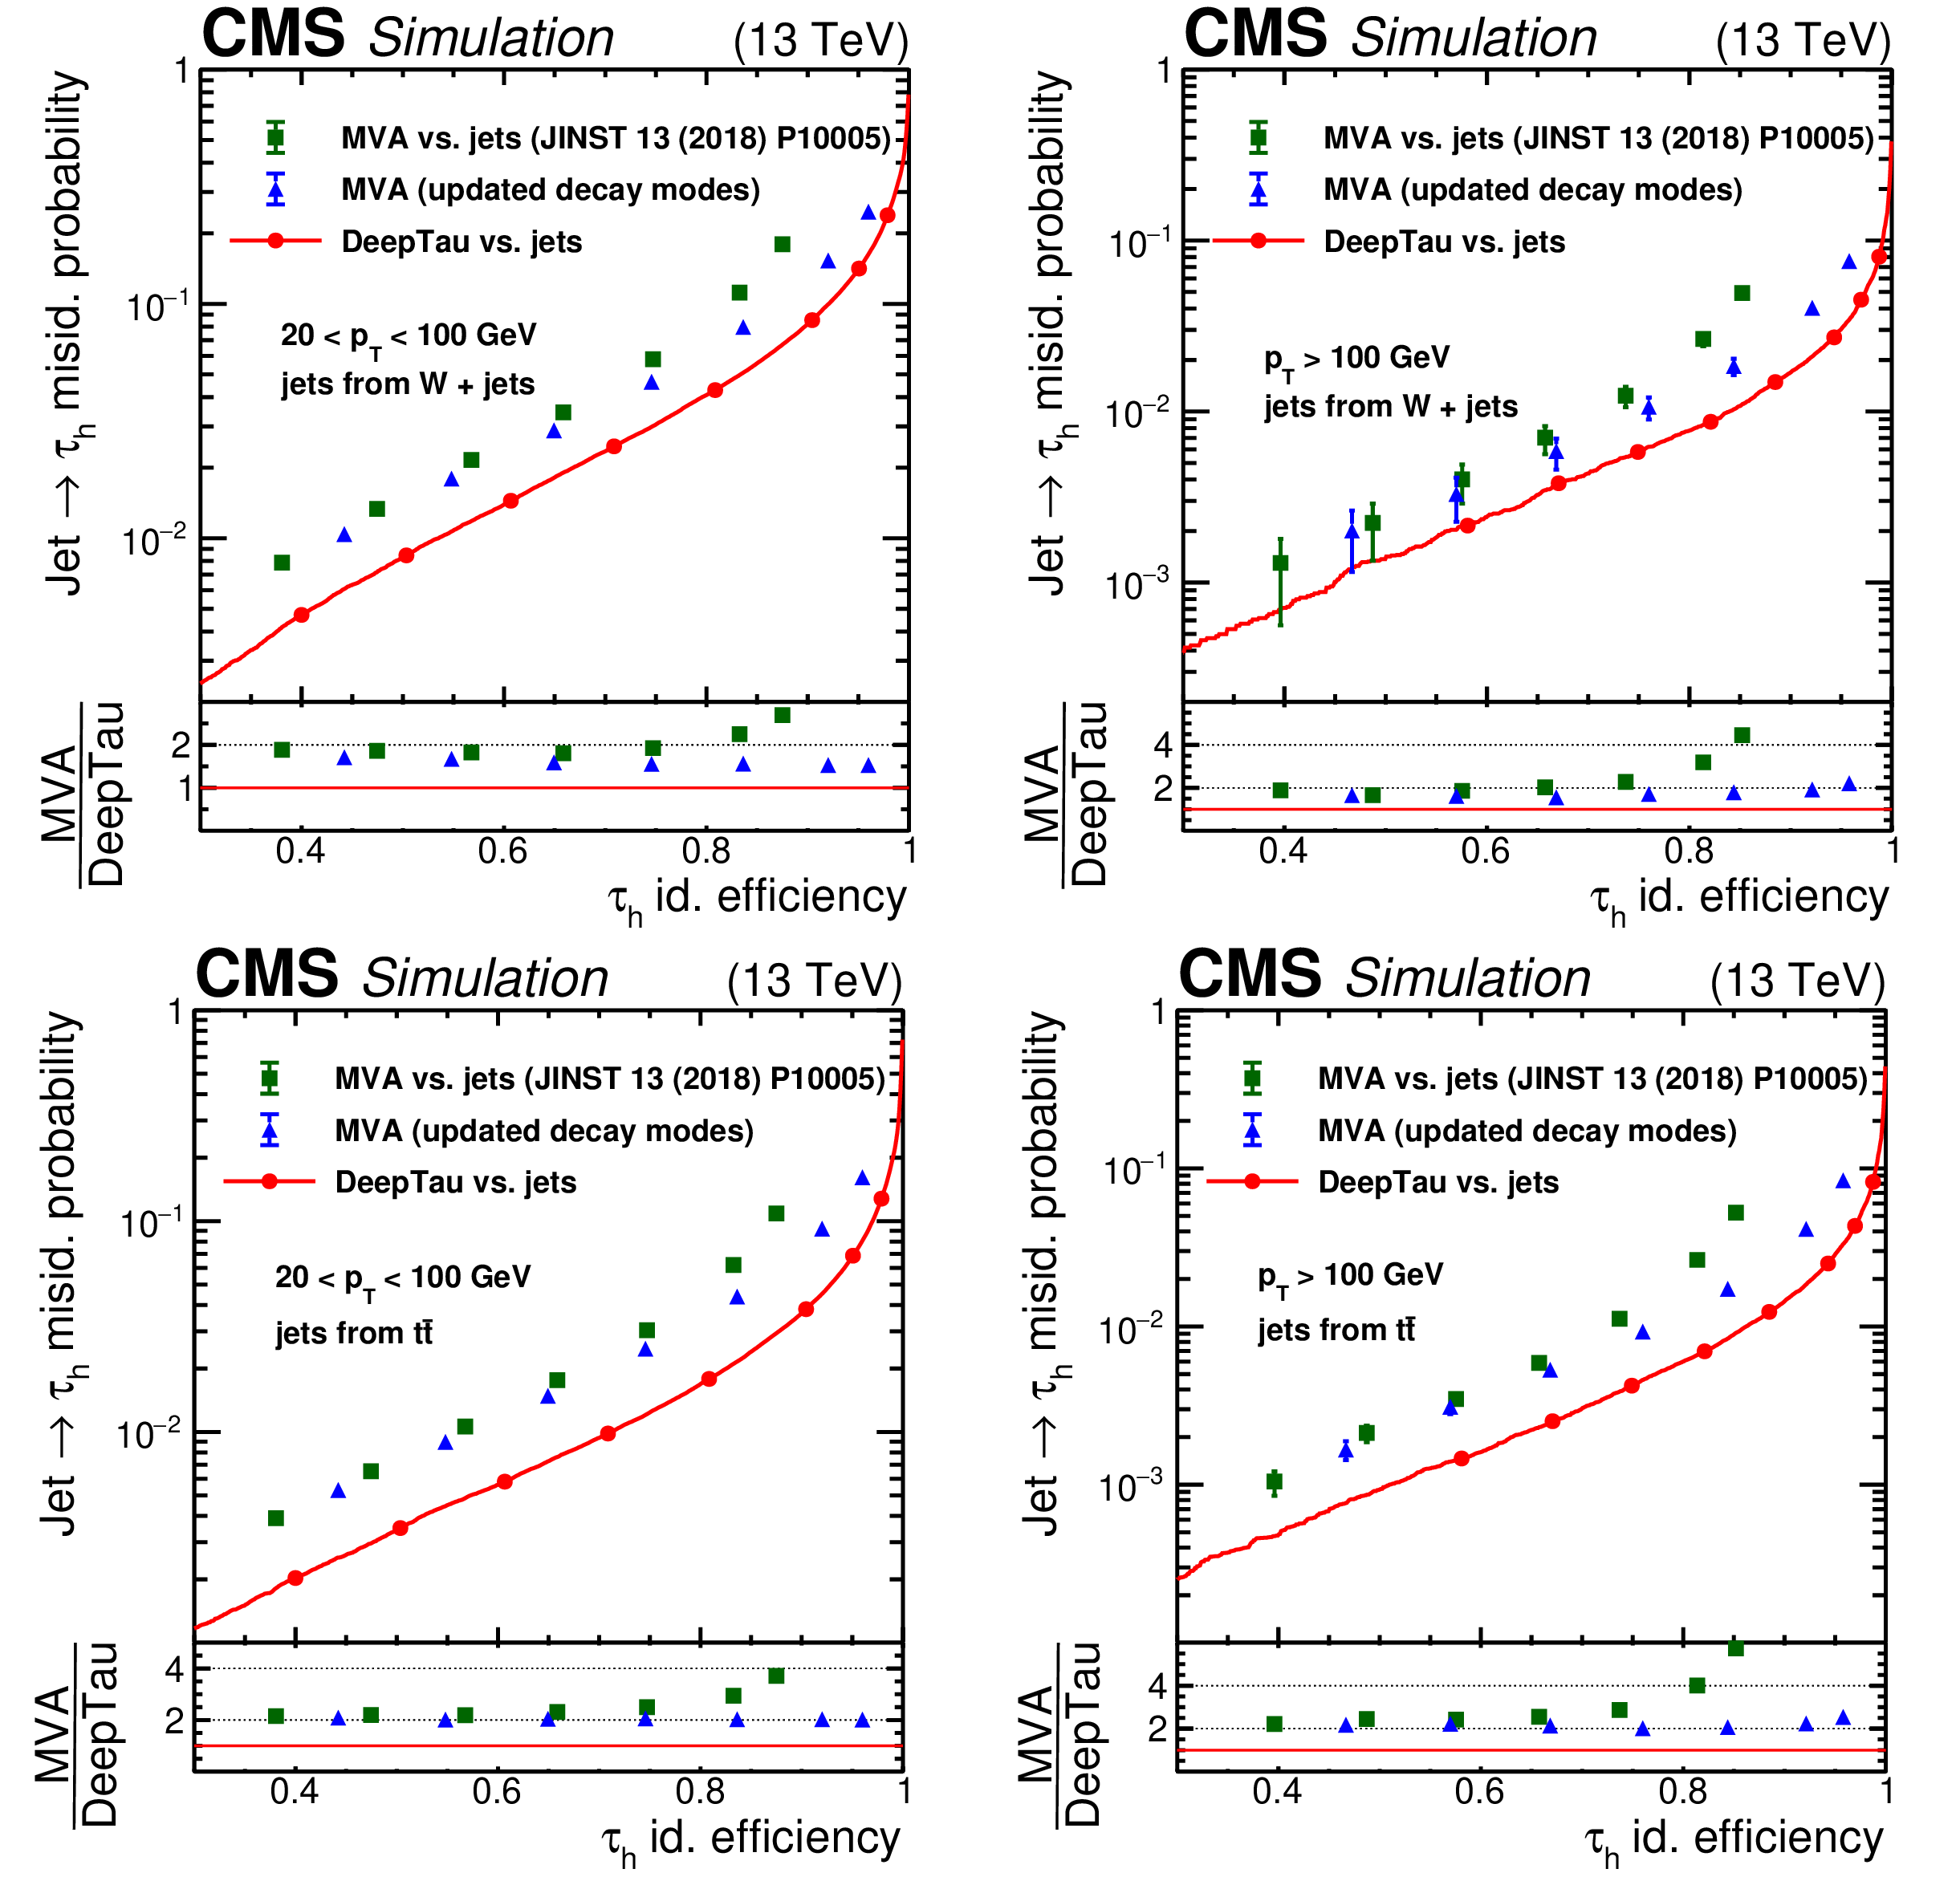
\includegraphics[scale=0.13]{Chapitre4/Images/DeepTauvsJets.png}
        \caption{}
    \end{subfigure}
    \begin{subfigure}[b]{\linewidth}
    \centering
        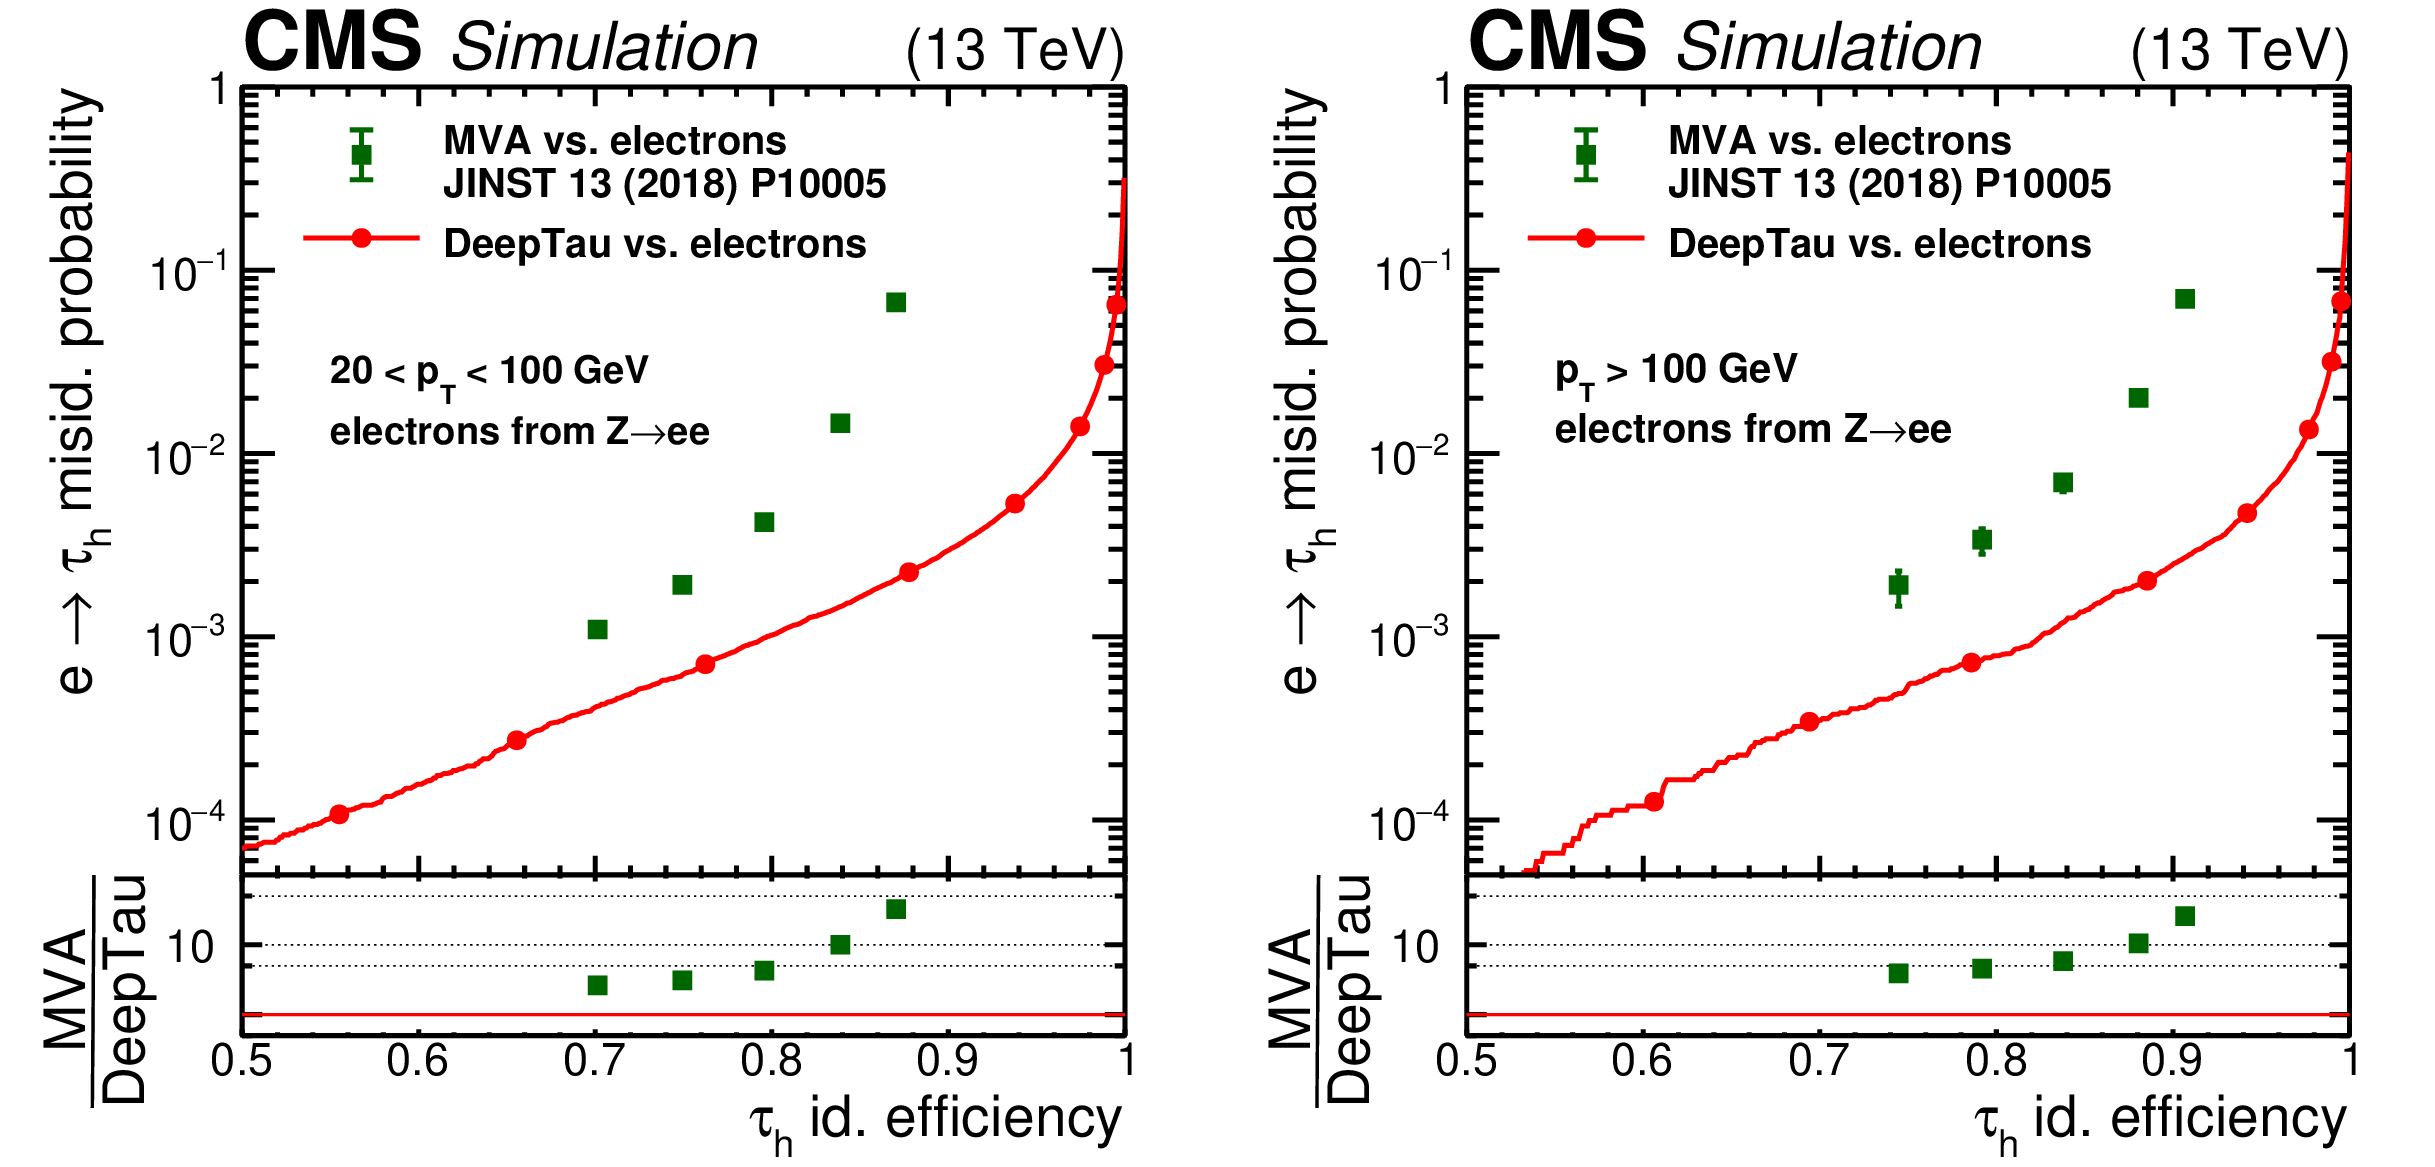
\includegraphics[scale=0.13]{Chapitre4/Images/DeepTauvsEle.png}
        \caption{}
    \end{subfigure}
    \begin{subfigure}[b]{\linewidth}
    \centering
        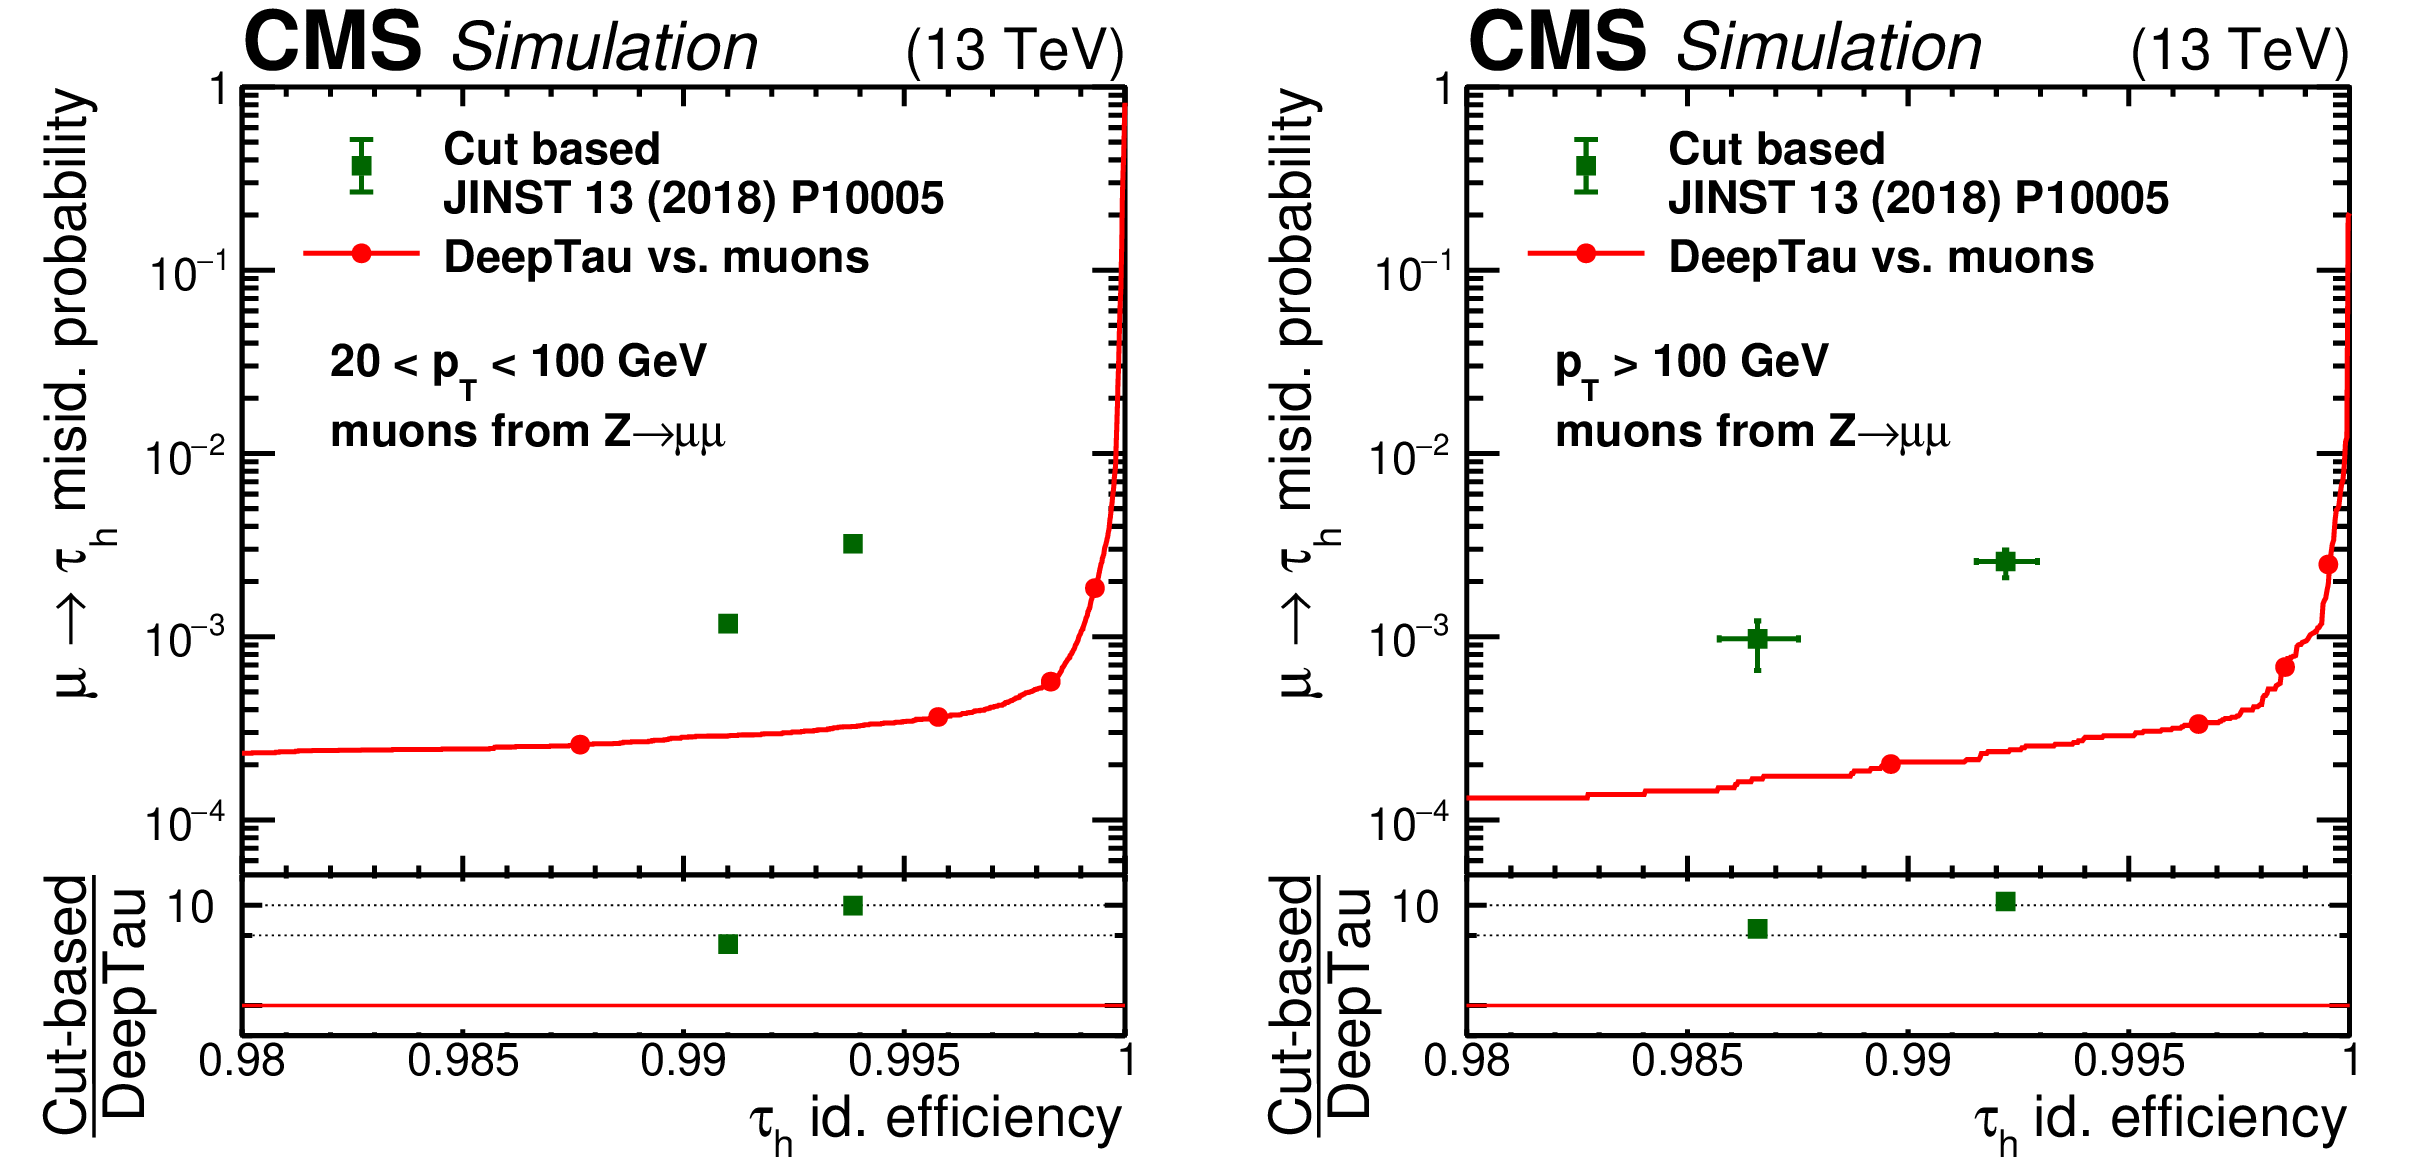
\includegraphics[scale=0.13]{Chapitre4/Images/DeepTauvsMu.png}
        \caption{}
    \end{subfigure}
    \caption{Probabilité de mauvaise identification d'un jet (a), d'un électron (b) ou d'un muon (c) en tau hadronique pour \textit{DeepTau} (rouge) et autres modes d'identification précedemment utilisés \cite{deeptau}.}
    \label{deeptauperf}
\end{figure}

\subsection{Modélisation du bruit de fond $Z\to\tau\tau$ (\textit{embedding})}
\label{embed}

Chaque mesure réalisée au LHC basée sur l'analyse d'un état final comportant des leptons tau est confrontée à un important bruit de fond provenant des désintégrations $Z\rightarrow\tau\tau$. Dans cette optique, une méthode visant à intégrer une paire de leptons tau simulés au sein d'événements $Z\rightarrow\mu\mu$ collectés par le détecteur CMS dans des collisions proton-proton a été mise au point \cite{Embedding}, et est notamment utilisée dans l'analyse des propriétés CP du boson de Higgs présentée dans cette thèse. Cette méthode permet de s'affranchir des difficultés de simulation de l'empilement et des gerbes hadroniques produites conjointement dans ce type d'événement en offrant des échantillons de données hybrides dans lesquels seuls les leptons tau sont simulés. Après une brève introduction de la méthode, des travaux visant à apporter une meilleure compréhension de certains évènements à haute MET seront présentés. \\ 


\begin{figure}
\centering
    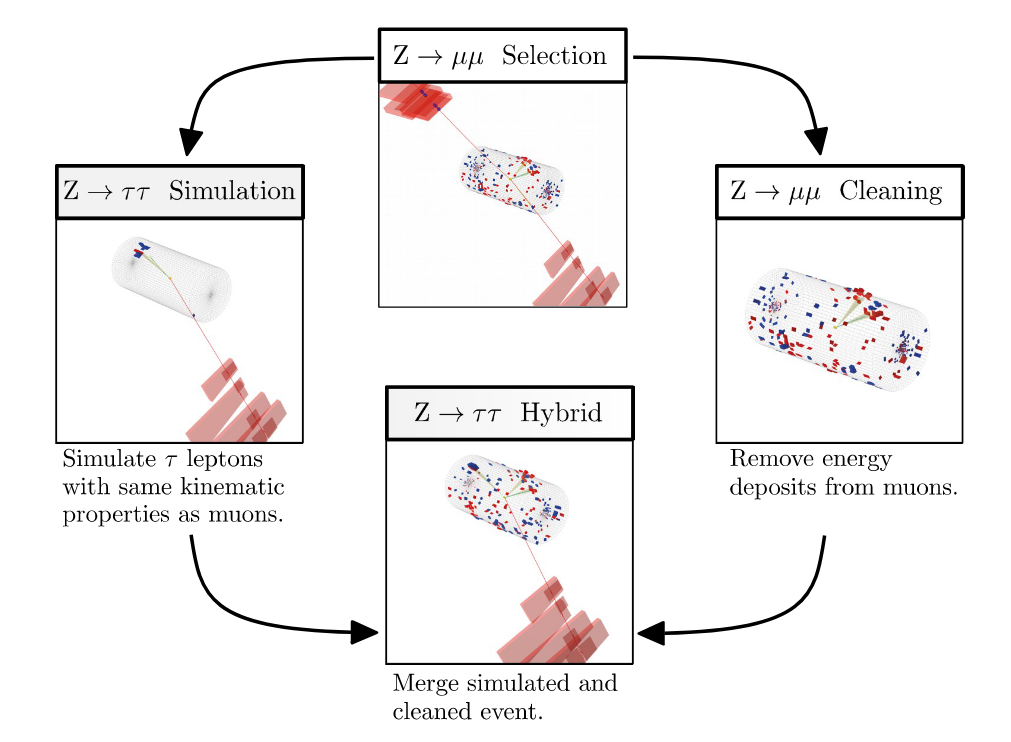
\includegraphics[scale=0.38]{Chapitre4/Images/4steps.png} 
    \caption{Intégration d'une paire de leptons tau simulés dans un événement $Z\rightarrow\mu\mu$ en 4 étapes : sélection (\textit{selection}), simulation (\textit{simulation}), nettoyage (\textit{cleaning}), regroupement (\textit{merging}) \cite{Embedding}.}
    \label{4steps}
\end{figure} 

La méthode d'intégration des leptons tau, appelée couramment $\textit{"embedding"}$, repose majoritairement sur l'hypothèse de l'universalité leptonique. Cette dernière stipule que les trois saveurs leptoniques sont équivalentes face au couplage faible, permettant de garantir qu'une désintégration $Z\rightarrow\tau\tau$ se déroulera dans un environnement sous-jacent parfaitement identique à celui d'une désintégration $Z\rightarrow\mu\mu$ et avec la même probabilité. En tenant aussi compte de l'excellente performance du détecteur CMS dans l'identification et la reconstruction des muons, il est alors possible de concevoir une méthode dans laquelle des événements $Z\rightarrow\mu\mu$ sont utilisés afin d'y intégrer une paire de leptons tau simulés avec les mêmes propriétés cinématiques. La production d'un événement hybride se déroule selon quatre étapes majeures décrites ci-dessous et résumées dans la figure \ref{4steps} :

\begin{enumerate}
    \medskip
    \item \textbf{Sélection} d'un évènement $Z\rightarrow\mu\mu$ dans les données.
    \medskip
    \item \textbf{Simulation} d'une paire de leptons tau avec des propriétés cinématiques équivalentes aux muons précédemment identifiés.
    \medskip
    \item \textbf{Nettoyage} des traces et des dépôts d'énergie des muons de l'événement sélectionné.
    \medskip
    \item \textbf{Regroupement} de l'événement nettoyé et de la paire simulée.
    \medskip
\end{enumerate}

Ce type d'échantillon est d'un intérêt particulier dans les analyses impliquant des désintégrations $Z\rightarrow\tau\tau$ puisqu'elle offre une meilleure description des données que les échantillons purement simulés. La figure \ref{embedindata} présente la distribution de quelques variables dans l'état final $\mu\tau_h$ ainsi que l'accord entre données et simulation dans les données de 2017. On remarque une amélioration globale de cet accord lorsque la contribution des évènements $Z\rightarrow\tau\tau$ est estimée grâce à \textit{l'embedding}. La section \ref{optvar} est dédiée à une étude des variables optimales de spin du lepton tau dans ces échantillons.  \\

\begin{figure}[!ht]
  \begin{subfigure}[b]{0.33\linewidth}
    \centering
    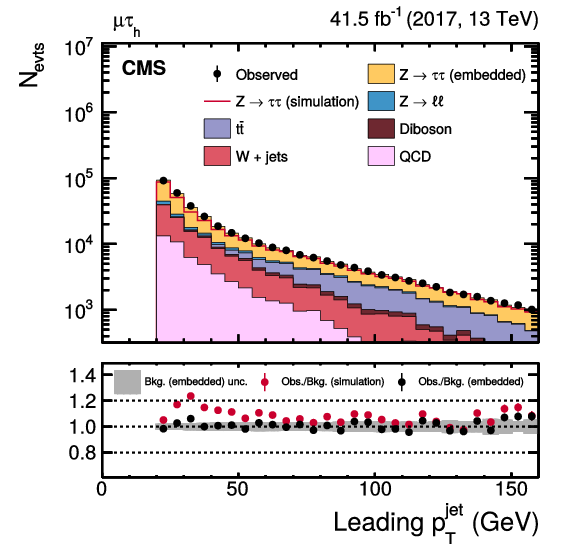
\includegraphics[width=\linewidth]{Chapitre4/Images/leadj_embed.png} 
    \caption*{} 
    \vspace{0.5ex}
  \end{subfigure}%% 
  \begin{subfigure}[b]{0.33\linewidth}
    \centering
    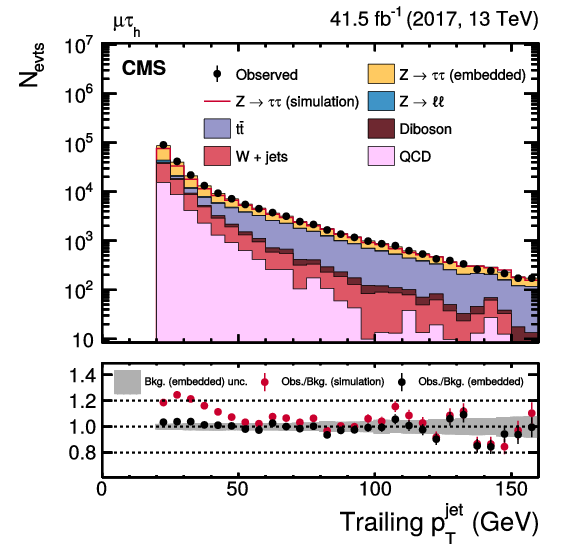
\includegraphics[width=\linewidth]{Chapitre4/Images/trailj_embed.png} 
    \caption*{} 
    \vspace{0.5ex}
  \end{subfigure} 
    \begin{subfigure}[b]{0.33\linewidth}
    \centering
    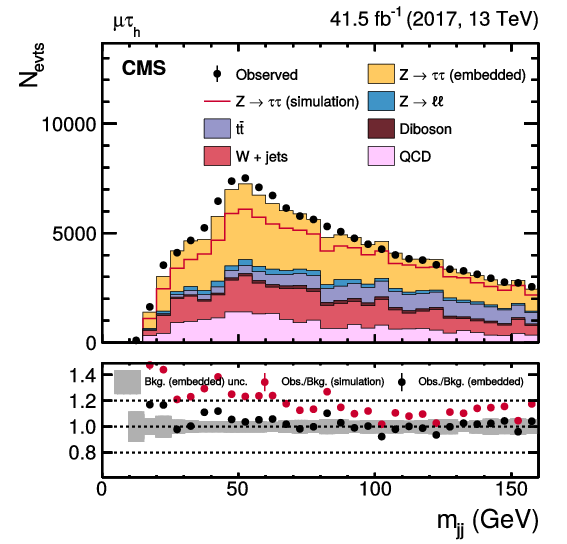
\includegraphics[width=\linewidth]{Chapitre4/Images/mjj_embed.png} 
    \caption*{} 
    \vspace{0.5ex}
  \end{subfigure} 

  \begin{subfigure}[b]{0.33\linewidth}
    \centering
    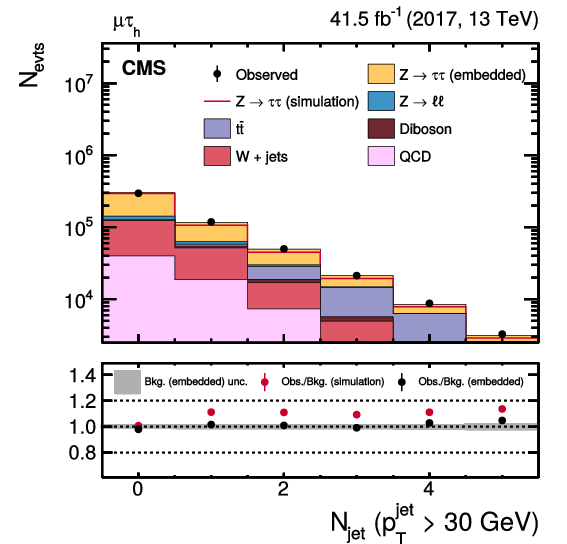
\includegraphics[width=\linewidth]{Chapitre4/Images/Njets_embed.png} 
    \caption*{} 
    \vspace{0.5ex}
  \end{subfigure}%% 
  \begin{subfigure}[b]{0.33\linewidth}
    \centering
    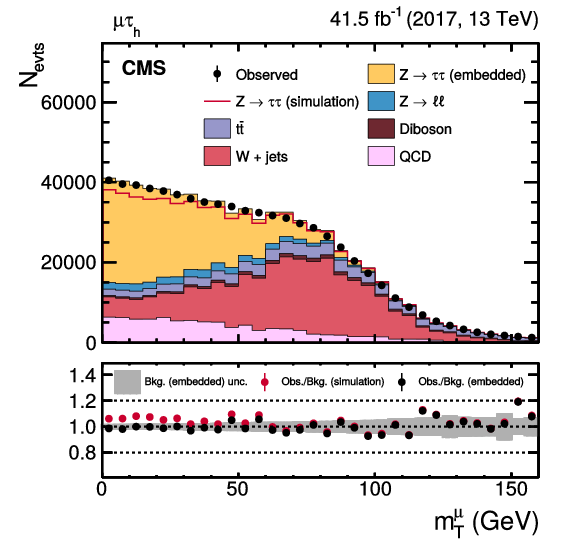
\includegraphics[width=\linewidth]{Chapitre4/Images/mtmu_embed.png} 
    \caption*{} 
    \vspace{0.5ex}
  \end{subfigure} 
    \begin{subfigure}[b]{0.33\linewidth}
    \centering
    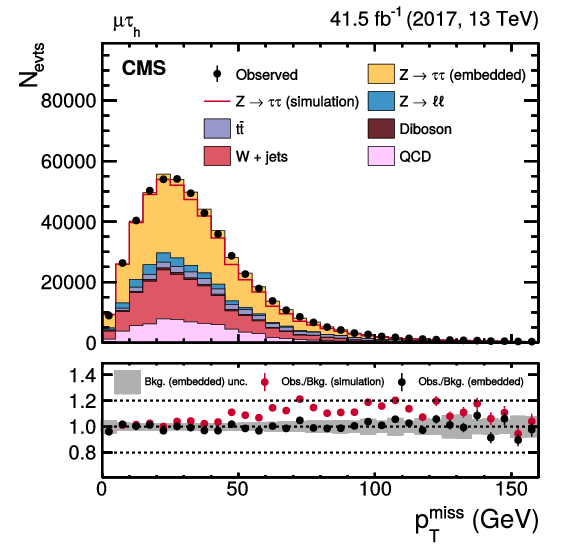
\includegraphics[width=\linewidth]{Chapitre4/Images/ptmiss_embed.png} 
    \caption*{} 
    \vspace{0.5ex}
  \end{subfigure} 
  \caption{Distribution de $p_T$ du jet de plus haute impulsion transverse (haut, gauche), $p_T$ du second jet de plus haute impulsion transverse (haut, centre), $m_{inv}$ de la paire de jets de plus haute impulsion transverse (haut, droite), $N_{jets}$ (bas, gauche), $m_T^{\mu}$ (bas, centre), $p_T^{miss}$ (bas, droite) dans l'état final $\mu\tau_h$. L'estimation de la contribution des évènements $Z\rightarrow\tau\tau$ issus des échantillons Monte Carlo est représentée par la ligne rouge \cite{Embedding}.}
  \label{embedindata}
\end{figure}

\section{Impact de l'identification des électrons et photons sur la reconstruction des leptons tau}

Une étude des performances de l'algorithme HPS a été réalisée au cours de cette thèse dans le cadre des EPR afin de mesurer l'impact de l'identification des électrons et des photons reconstruits par le flux de particules sur la reconstruction des leptons tau. Lors du démarrage du Run 2, une perte d'efficacité de reconstruction du mode de désintégration $\tau_h\rightarrow\pi^{\pm}+\pi^0s$ (DM1+DM2) de l'ordre de $5-10\%$ en comparaison avec les performances du Run 1 fut observée. Cette perte est attribuée au déploiement d'une nouvelle méthode d'identification des photons s'appuyant sur un réseau de neurone ($e/\gamma$-ID) au cours de laquelle les photons convertis en paire électron/positron peuvent être reconstruits à partir d'une seule trace lorsque la seconde est perdue (\textit{single-track photon conversions}). Lors de cette identification, plusieurs éléments tels que les traces ou dépôts d'énergie de hadrons ($\pi^{\pm},\pi^0$) peuvent être faussement associés à des photons, tandis qu'un effet similaire mais réduit est observé pour le mode de désintégration $\tau_h\rightarrow\pi^{\pm}$ (DM0). Cette étude permet d'évaluer les performances du $e/\gamma$-ID, ré-entraîné en prévision du Run 3, et de s'assurer que son utilisation n'entraîne pas de perte de performance supplémentaire dans l'identification des leptons tau. \\

\begin{figure}[!ht]
\captionsetup{justification=centering}
  \begin{subfigure}{0.5\linewidth}
    \centering
    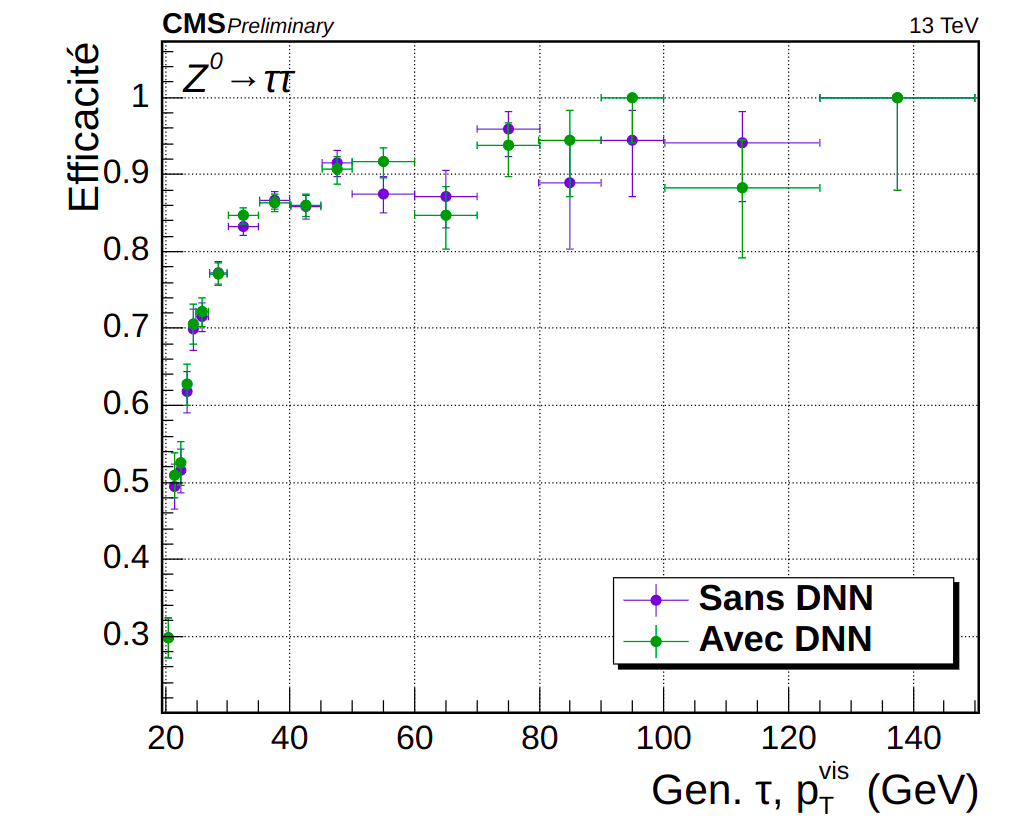
\includegraphics[width=0.8\linewidth]{Chapitre4/Images/HPSnewDMs_ztt_pt.png} 
    \caption{Efficacité vs $p_T^{\text{vis}}$ dans l'échantillon \\ $Z\rightarrow\tau\tau$} 
  \end{subfigure}
  \begin{subfigure}{0.5\linewidth}
    \centering
    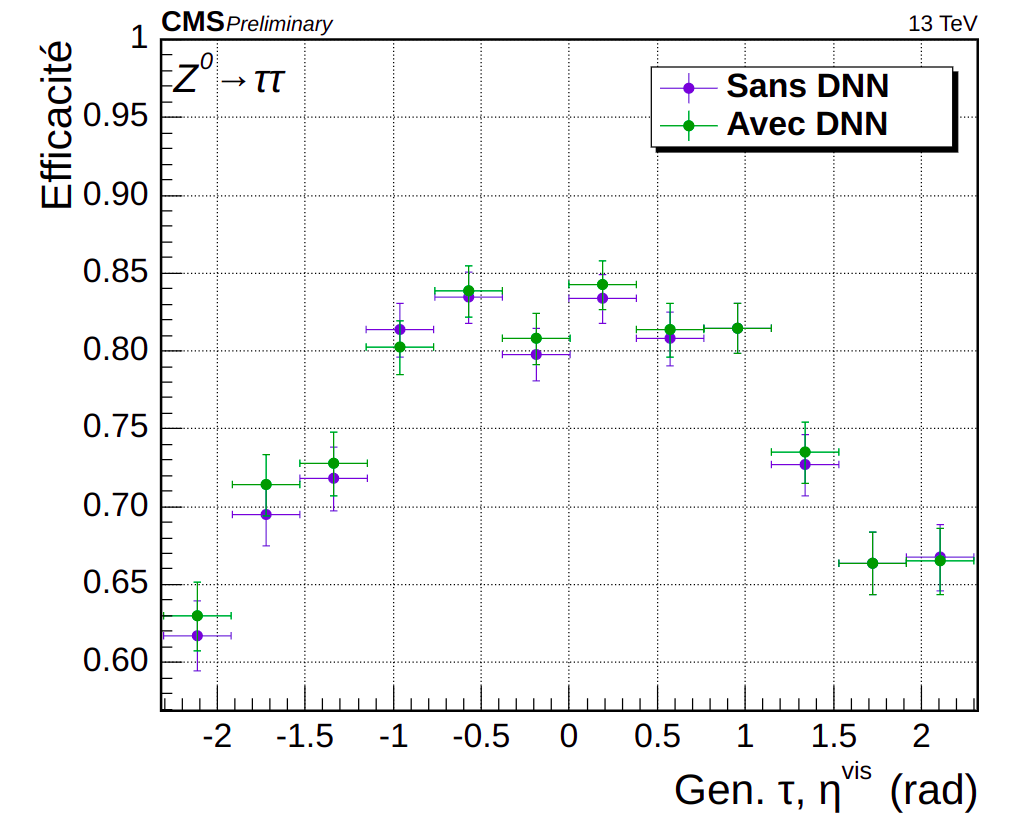
\includegraphics[width=0.8\linewidth]{Chapitre4/Images/HPSnewDMs_ztt_eta.png} 
    \caption{Efficacité vs $\eta^{\text{vis}}$ dans l'échantillon \\ $Z\rightarrow\tau\tau$} 
  \end{subfigure} 
  \begin{subfigure}{0.5\linewidth}
    \centering
    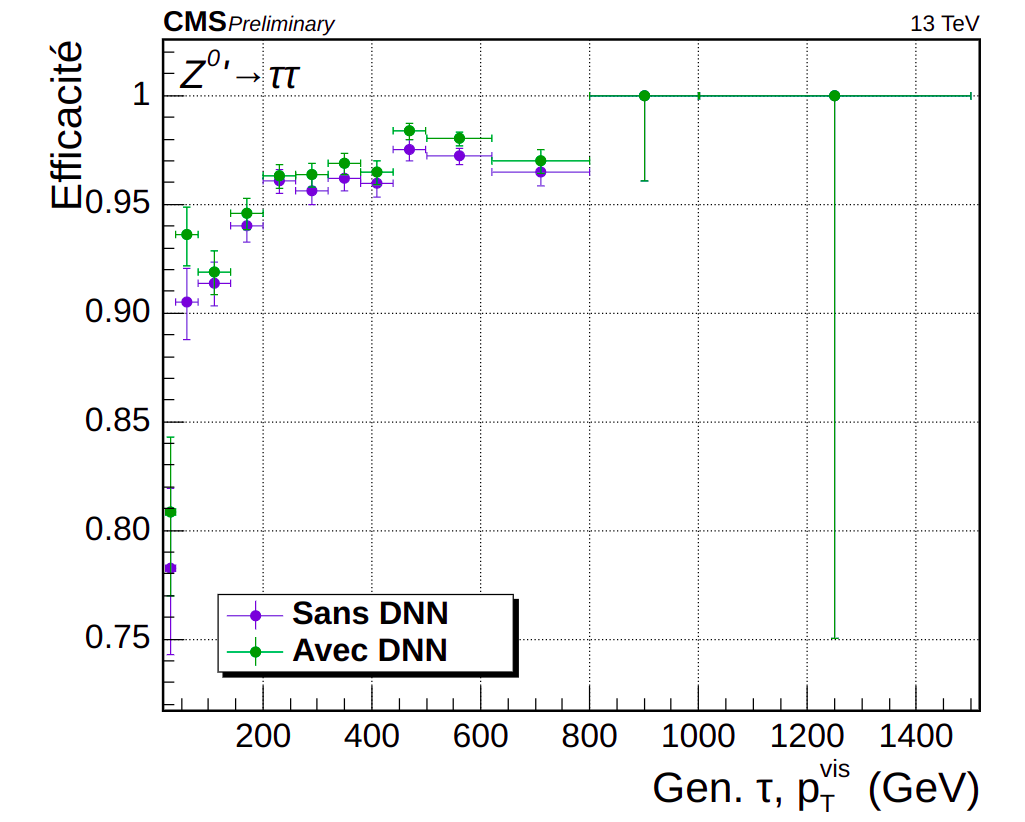
\includegraphics[width=0.8\linewidth]{Chapitre4/Images/HPSnewDMs_zptt_pt.png} 
    \caption{Efficacité vs $p_T^{\text{vis}}$ dans l'échantillon \\ $Z'\rightarrow\tau\tau$} 
  \end{subfigure}
  \begin{subfigure}{0.5\linewidth}
    \centering
    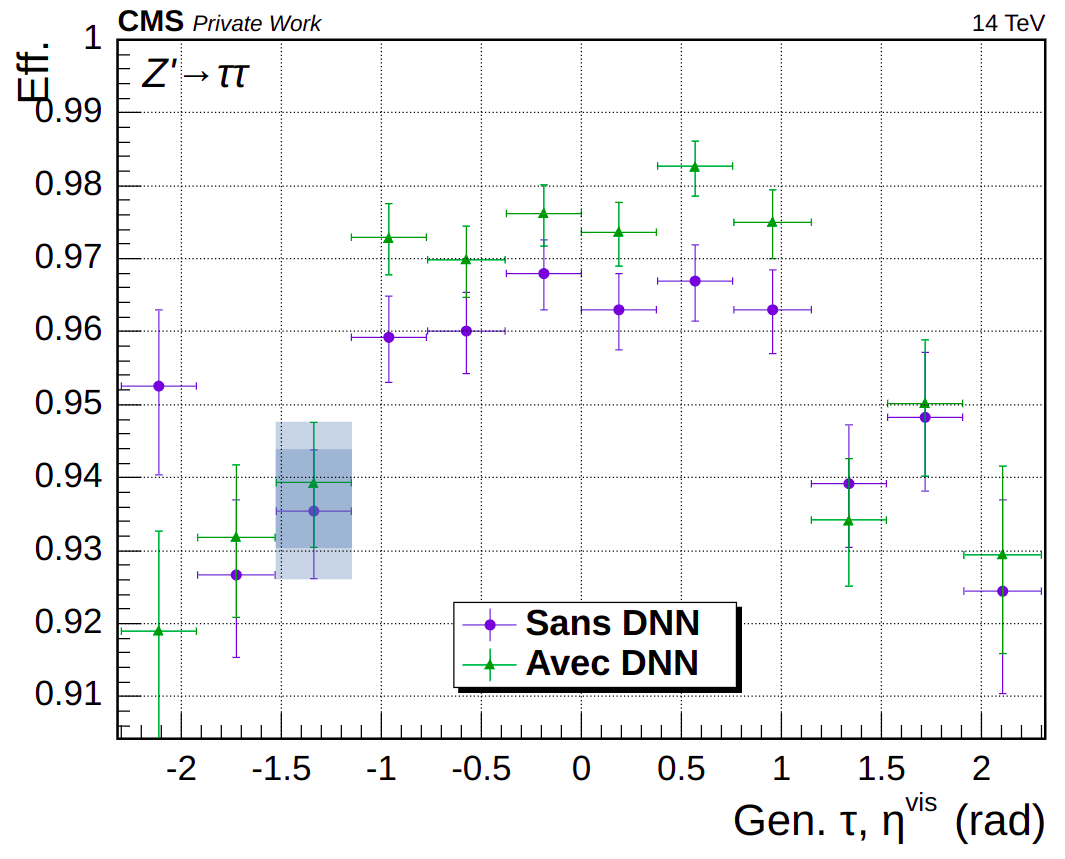
\includegraphics[width=0.8\linewidth]{Chapitre4/Images/HPSnewDMs_zptt_eta.png} 
    \caption{Efficacité vs $\eta^{\text{vis}}$ dans l'échantillon \\ $Z'\rightarrow\tau\tau$} 
  \end{subfigure}
  \begin{subfigure}{0.5\linewidth}
    \centering
    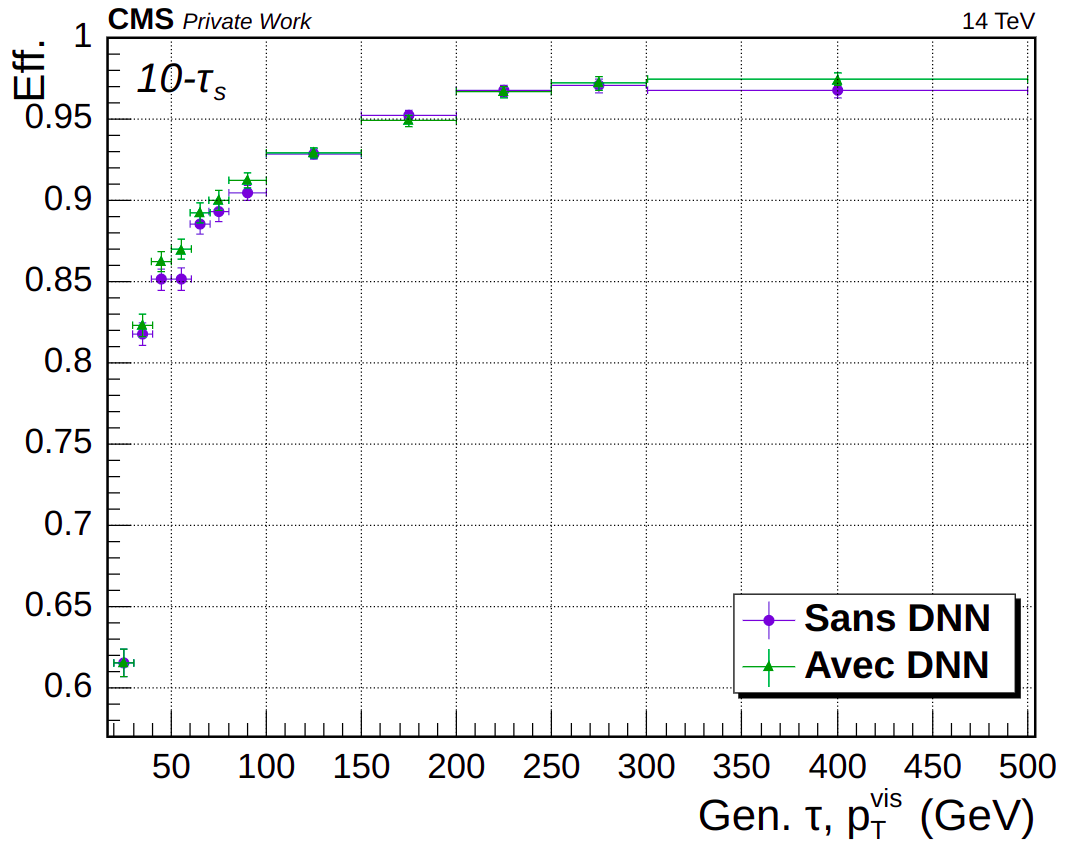
\includegraphics[width=0.8\linewidth]{Chapitre4/Images/HPSnewDMs_10t_pt.png} 
    \caption{Efficacité vs $p_T^{\text{vis}}$ dans l'échantillon \\ "\textit{TauGun}"} 
  \end{subfigure}
  \begin{subfigure}{0.5\linewidth}
    \centering
    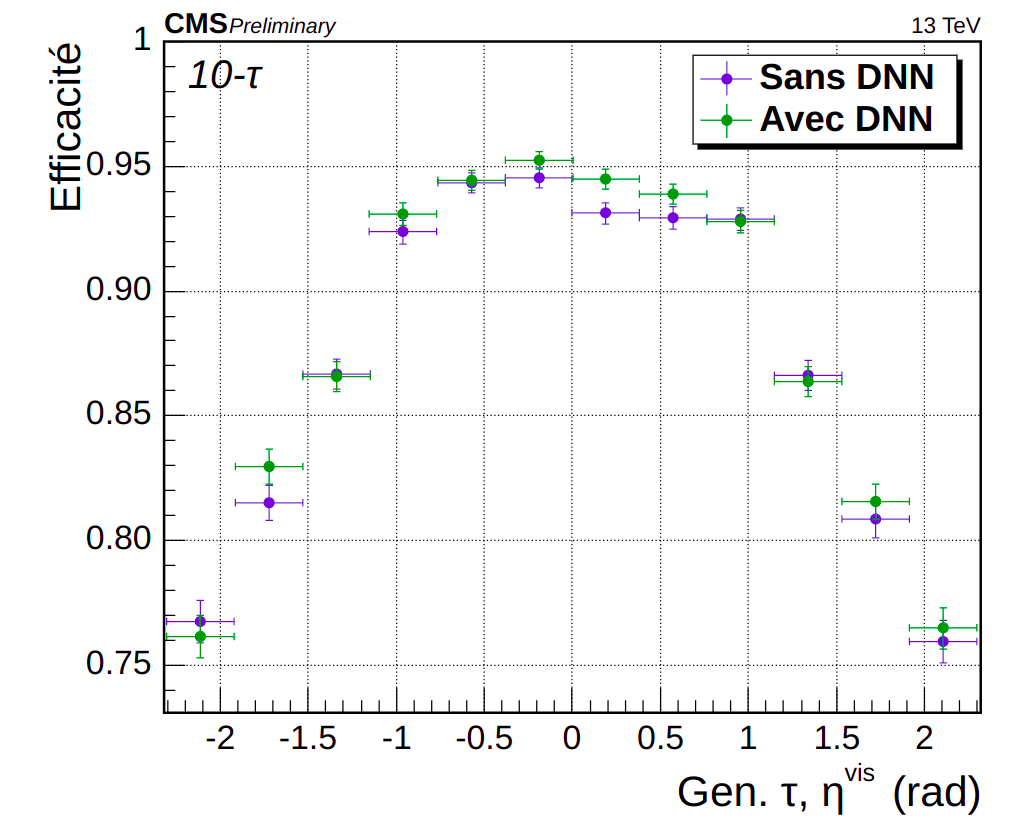
\includegraphics[width=0.8\linewidth]{Chapitre4/Images/HPSnewDMs_10t_eta.png} 
    \caption{Efficacité vs $\eta^{\text{vis}}$ dans l'échantillon \\ "\textit{TauGun}"} 
  \end{subfigure} 
  \caption{Efficacité de l'algorithme HPS en fonction de $p_T^{\text{vis}}$ et $\eta^{\text{vis}}$ des leptons tau générés.}
  \label{TenTaus1}
\end{figure}

\begin{figure}[!ht]
  \begin{subfigure}{0.5\linewidth}
    \centering
    \includegraphics[width=1\linewidth]{Chapitre4/Images/DMmatrices/Matrix_DNNDisabled.png} 
    \caption{Échantillon $Z\rightarrow\tau\tau$, sans DNN.}
    \vspace{0.5ex}
  \end{subfigure}
  \begin{subfigure}{0.5\linewidth}
    \centering
    \includegraphics[width=1\linewidth]{Chapitre4/Images/DMmatrices/Matrix_DNNEnabled.png} 
    \caption{Échantillon $Z\rightarrow\tau\tau$, avec DNN.}
    \vspace{0.5ex}
  \end{subfigure} 
  \begin{subfigure}{0.5\linewidth}
    \centering
    \includegraphics[width=1\linewidth]{Chapitre4/Images/DMmatrices/Matrix_DNNDisabled_ZpTT.png} 
    \caption{Échantillon $Z'\rightarrow\tau\tau$, sans DNN.}
    \vspace{0.5ex}
  \end{subfigure}
  \begin{subfigure}{0.5\linewidth}
    \centering
    \includegraphics[width=1\linewidth]{Chapitre4/Images/DMmatrices/Matrix_DNNEnabled_ZpTT.png} 
    \caption{Échantillon $Z'\rightarrow\tau\tau$, avec DNN.}
    \vspace{0.5ex}
  \end{subfigure} 
  \begin{subfigure}{0.5\linewidth}
    \centering
    \includegraphics[width=1\linewidth]{Chapitre4/Images/DMmatrices/Matrix_DNNDisabled_10taus.png} 
    \caption{Échantillon "\textit{TauGun}", avec DNN.}
    \vspace{0.5ex}
  \end{subfigure}
  \begin{subfigure}{0.5\linewidth}
    \centering
    \includegraphics[width=1\linewidth]{Chapitre4/Images/DMmatrices/Matrix_DNNEnabled_10taus.png} 
    \caption{Échantillon "\textit{TauGun}", sans DNN.}
    \vspace{0.5ex}
  \end{subfigure} 
  \caption{Matrices de confusion des modes de désintégration HPS normalisées par lignes.}
  \label{DMmatrix}
\end{figure}

Trois échantillons de données simulés ont été utilisés pour cette étude : un premier comportant des événements $Z\rightarrow\tau\tau$ tels que décrits par le modèle standard produits dans des collisions $pp$ à $\sqrt{s}=14$ TeV avec des leptons tau couvrant une plage d'impulsion transverse allant de $20$ à $150$ GeV, un second analogue avec un boson $Z'$ plus lourd permettant de couvrir une plage d'impulsion transverse atteignant $1500$ GeV et enfin un sample "\textit{TauGun}" dans lequel des leptons taus sont simulés uniformément avec une impulsion transverse variant de $15$ à $500$ GeV à raison de dix leptons tau par événement. La figure \ref{TenTaus1} présentent la distribution de l'efficacité de l'algorithme HPS en fonction de l'impulsion transverse et de la coordonné $\eta$ de la partie visible des taus simulés dans les trois échantillons. Dans ce cadre, l'efficacité est définie comme la proportion de taus reconstruits avec un mode de désintégration correctement attribué ou non. Ces distributions montrent que l'efficacité de reconstruction des leptons tau obtenue avec le $e/\gamma$-ID est compatible avec celle lorsque ce dernier n'est pas employé et que le nouvel entraînement ne provoque pas de perte d'efficacité supplémentaire. La figure \ref{DMmatrix} montre les matrices de confusion pour chaque modes de désintégration normalisées par lignes. La pureté des modes désintégration $\tau_h\rightarrow\pi^{\pm}+\pi^0s$ (DM1+DM2) est améliorée d'environ $15\%$ dans les échantillons $Z^{0'}$ et "\textit{TauGun}". La figure \ref{DM12} montre quant à elle que cette amélioration a en effet principalement lieu à haute impulsion transverse entre $100$ et $200$ GeV, justifiant un effet moins moindre au sein de l'échantillon $Z\rightarrow\tau\tau$. 





En conclusion, le nouveau $e/\gamma$-ID présenté offre des performances stables vis à vis de l'identification des leptons tau sans néanmoins recouvrir l'efficacité perdue lors entre le Run 1 et le Run 2.

\begin{figure}
  \begin{subfigure}{0.5\linewidth}
    \centering
    \includegraphics[width=\linewidth]{Chapitre4/Images/HPSnewDM12s_zptt_pt.png} 
  \end{subfigure}
  \begin{subfigure}{0.5\linewidth}
    \centering
    \includegraphics[width=\linewidth]{Chapitre4/Images/HPSnewDM12s_10t_pt.png} 
  \end{subfigure} 
  \caption{Efficacité vs $p_T^{\text{vis}}$ dans l'échantillon $Z'\rightarrow\tau\tau$ (gauche) et "\textit{TauGun}" (droite) pour les modes de désintégration 1 et 2.}
  \label{DM12}
\end{figure}
    %\chapter{Violation de CP dans le secteur du Higgs}
\label{violCP}

La symétrie CP représente un \textit{miroir} à travers lequel la matière devient antimatière par action conjointe des opérateurs de charge $(\hat{C})$ et de parité $(\hat{P})$. Le premier a pour effet de transformer une particule en son anti-particule en inversant le signe de sa charge électrique tandis que le second, tel qu'introduit dans le paragraphe \ref{weakinter}, inverse ses coordonnées spatiales. La naissance de l'Univers fut accompagnée d'une création de matière et d'anti-matière, formant dans ses tout premiers instants des baryons et des anti-baryons à l´équilibre thermique avec les photons de haute énergie peuplant l'Univers primitif par des annihilations et créations successives : $$\gamma+\gamma\Longleftrightarrow \mbox{p}+\overline{\mbox{p}}.$$ 
Dans les instants suivants, le refroidissement de l'Univers a entraîné l'arrêt de ces réactions en fixant en quantité égale le nombre de baryons et d'anti-baryons alors présents. Aujourd'hui, les observations témoignent d'une disparition quasi totale de l'antimatière, montrant que des mécanismes ne conservant pas la symétrie CP ont eu lieu dans les premières phases de l'Univers. Bien que des sources de violation CP soient effectivement observées dans des mécanismes prédits par le modèle standard dans le secteur des quarks \cite{Fritzsch_1999}, elles sont néanmoins insuffisantes pour justifier l'asymétrie matière-antimatière actuelle. En particulier, toutes les interactions du boson de Higgs étant décrites comme invariantes sous une transformation CP et à travers des couplages de type scalaire, toute découverte de violation dans ce secteur représenterait une forte indication de l'existence de nouvelle physique. 

\section{Couplages du boson de Higgs}
\label{decays}


\begin{figure}
\centering
    \includegraphics[scale=0.4]{Chapitre5/Images/Hgammagamma.png} 
    \caption{Distribution de la masse invariante diphoton $m_{\gamma\gamma}$ dans les données de la première phase d'exploitation du LHC où chaque évènement est pondéré par son ratio de signal sur signal + bruit de fond S/(S+B) \cite{higgsCMS1}.}
    \label{higgsGG}
\end{figure}

La découverte annoncée en 2012 par les collaborations ATLAS et CMS \cite{CMSdiscovery,ATLASdiscovery},constitue à elle seule une preuve solide de l'existence du boson de Higgs tel que prédit par le mécanisme de Higgs introduit dans le paragraphe \ref{higgsmeca}. La première mesure de sa masse par l'expérience CMS lors de sa découverte est de $m_{H}=125,3\pm0,4(stat.)\pm0,5(syst.)$ GeV dans les canaux $H\rightarrow ZZ\rightarrow 4\ell$ et $H\rightarrow \gamma\gamma$ où l'excès est le plus significatif (Fig. \ref{higgsGG}). Le mode de désintégration en paire de photons permet également de confirmer que la particule observée est un boson de spin différent de 1 et de charge nulle. Les dernières mesures de sa masse par l'expérience CMS offrent désormais une précision à l'ordre du millième avec une valeur $m_{H}=125,38\pm0,14$ GeV dans le canal $H\to\gamma\gamma$ mesurée en 2020 \cite{HiggsMass2020}, puis $m_{H}=125,08\pm0,12$ GeV dans le canal $H\to ZZ\to 4\ell$ mesurée en 2023 \cite{HiggsMass2023}. Parmi les modes de production du boson de Higgs prédits par le modèle standard, 87\% de la section efficace de production au LHC sont attribués à la fusion d'une paire de gluons à travers une boucle quantique de quarks top virtuels (Fig. \ref{Hdecays}.a). Le second mode de production est celui mettant en jeu une fusion de deux bosons vecteurs (Fig. \ref{Hdecays}.b), chacun radié par un des quarks des protons entrés en collision. D'autres modes de production en association avec un boson vecteur (Fig. \ref{Hdecays}.c), ou des quarks de troisième génération (Fig. \ref{Hdecays}.d-f) sont également prédits avec une contribution mineure à la section efficace totale. Le temps de vie du boson de Higgs prédit par le modèle standard est de $\tau_H\approx1,6.10^{-22}$ s, correspondant à une largeur de désintégration $\Gamma_{H}=\hbar/\tau_{H}=4,14\pm0.02$ MeV, définie comme la somme des largeurs de désintégration partielles de tous les modes de désintégration et où $\hbar=h/2\pi$ est la constante de Planck réduite. Dans le modèle standard, ces désintégrations se produisent à travers un couplage à une paire de bosons ou de fermions avec une amplitude proportionnelle à la masse, rendant notamment le couplage aux particules de 3ème génération plus fort. La mesure de la largeur de désintégration est une tâche importante puisqu'une déviation de cette dernière de sa valeur prédite serait une indication directe de nouvelle physique. À ce jour, la mesure réalisée par l'expérience CMS est en accord avec le modèle standard avec une valeur $\Gamma_{H}=3,2^{+2,4}_{-1,7}$ MeV \cite{HiggsWidth2022}. D'autre part, l'expérience CMS observe désormais la désintégration du boson de Higgs en une paire de leptons tau avec $5,9\sigma$, sa désintégration en une paire de quarks $b$ avec $5,6\sigma$, son mode de production associé à une paire de quarks $t$ ($ttH$) avec $5,2\sigma$ et enfin sa désintégration en paire de muons avec $3,0\sigma$ \cite{higgs10years}. Une autre façon de vérifier les prédictions du modèle standard consiste à mesurer une série de paramètres $\kappa$ appelés modificateurs de couplage et associés à chaque vertex faisant intervenir un boson de Higgs (Fig. \ref{Hdecays}). Ces paramètres, dont la valeur prédite dans le modèle standard est de 1 pour tous les couplages, agissent comme des facteurs d'échelle sur les sections efficaces de production et les taux de désintégration du boson de Higgs entre valeurs prédites et valeurs mesurées. La figure \ref{Cmodifiers} présente une mesure des paramètres $\kappa_{V}$ et $\kappa_f$ associés aux couplages aux bosons et fermions massifs respectivement, de la découverte en 2012 à la mesure la plus récente. La mesure des paramètres de couplage individuels pour les bosons $W$ et $Z$, les fermions de 3ème génération et le muon sont également présentés.

\begin{figure}
\centering
    \includegraphics[scale=0.4]{Chapitre5/Images/Hdecays.png} 
    \caption{Diagrammes de Feynmann des (a-f) modes de production du boson de Higgs et des (g-j) modes de désintégration du boson de Higgs \cite{higgs10years}.}
    \label{Hdecays}
\end{figure}

\begin{figure}
\centering
    \includegraphics[scale=0.25]{Chapitre5/Images/Cmodifiers.png} 
    \caption{Gauche : contraintes sur la mesure des modificateurs de couplages des fermions ($\kappa_f$) et bosons ($\kappa_V$) depuis sa découverte (rouge), après le Run 1 (bleu) et jusqu'à dix ans après sa découverte (noir). La prédiction du modèle standard est indiquée par le losange jaune. Droite : mesure des modificateurs de couplage bosons vecteurs (noir), des fermions de troisième génération (rouge) et du muon (bleu) en fonction de leur masse \cite{higgs10years}.}
    \label{Cmodifiers}
\end{figure}


\section{Couplage CP impair anomal aux bosons de jauge}
\label{anomalous}

D'après la section \ref{decays}, le boson de Higgs est capable de se coupler aux bosons vecteurs à travers le mode de désintégration $H\rightarrow VV$. Le système final est constitué de deux bosons de nature identique d'état de spin-parité $J^P=1^-$ et possède un moment orbital angulaire total pair tenant compte du spin nul du boson de Higgs initial. Avec ces considérations, le système final est contraint de posséder un état de parité pair, impliquant également une parité paire pour le boson de Higgs dans le cas où la désintégration est invariante sous une transformation CP. Une des analyses de l'expérience CMS menée en 2014 \cite{Z4lCP} porte sur la recherche de violation CP dans le couplage du boson de Higgs au boson $Z$ à travers le mode de désintégration $H\rightarrow ZZ\rightarrow 4l$. La forme la plus générale de l'amplitude de désintégration en paire de bosons vecteurs s'écrit :

\begin{equation}
    \mathcal{A}(H\rightarrow ZZ)=v^{-1}\bigl(a_1m^2_Z\epsilon^*_1\epsilon^*_2+a_2f^{*(1)}_{\mu\nu}f^{*(2),\mu\nu}+a_3f^{*(1)}_{\mu\nu}\tilde{f}^{*(2),\mu\nu}\bigr),
    \label{HZZdecay}
\end{equation}

où $m_Z$ est la masse du boson $Z$, $f^{(i),\mu\nu}=\epsilon_i^{\mu}q_i^{\nu}-\epsilon_i^{\nu}q_i^{\mu}$ est le tenseur champ d'un boson de jauge d'impulsion $q_i$ et de polarisation $\epsilon_i$, $\tilde{f}^(i)_{\mu\nu}\sfrac{1}{2}\epsilon_{\mu\nu\alpha\beta}f^{(i),\mu\nu}$ est le tenseur champ conjugué, $f^*$ son conjugué complexe et $v$ est la v.e.v du champ de Higgs. Les coefficients $a_i$ sont associés à différents couplages. L'amplitude de désintégration est dominée par le couplage associé à $a_1$ pour un couplage CP pair et à $a_3$ pour un couplage CP impair. Afin de mesurer l'accord des données avec une hypothèse de spin-parité quelconque $J^P$ face à celle du modèle standard définie par $J^P=0^+$, on introduit la variable de décision $q$ définie par :

\begin{equation}
    q=-2\ln \frac{\mathcal{L}_{J^P}}{\mathcal{L}_{0^+}},
\end{equation}

où $\mathcal{L}_{J^P}$ est une fonction de vraisemblance associée à l'hypothèse de spin-parité $J^P$ et $\mathcal{L}_{0^+}$ la fonction de vraisemblance associée à l'hypothèse purement scalaire. La figure \ref{statTest} montre la distribution de $q$ attendue pour l'hypothèse purement scalaire en jaune et purement pseudo-scalaire en bleu réalisée à travers de pseudo-expériences simulées. Pour l'hypothèse scalaire (pseudo-scalaire), la fonction de vraisemblance associée est construite en fixant la valeur de tous les coefficients $a_i$ de l'amplitude de désintégration \ref{HZZdecay} à $0$ à l'exception de $a_1$ ($a_3$). La valeur $q_{\text{obs}}$ observée dans les données est marquée par une flèche rouge et favorise de façon claire l'hypothèse purement scalaire en excluant l'hypothèse pseudo-scalaire à $3,8\sigma$.  

\begin{figure}
\centering
    \includegraphics[scale=0.3]{Chapitre5/Images/testStat.png} 
    \caption{Distribution de la variable de décision $q=-2\ln \frac{\mathcal{L}_{0^-}}{\mathcal{L}_{0^+}}$ pour l'hypothèse purement pseudo-scalaire (bleu) face à l'hypothèse purement scalaire (jaune). La flèche rouge indique la valeur observée dans les données du Run 1 \cite{Z4lCP}.}
    \label{statTest}
\end{figure}

\section{Violation de CP dans les couplages de Yukawa}

 Le Lagrangien \ref{yukawacoupling} introduit dans la section \ref{yukawa} reflétant le couplage entre le champ de Higgs et chaque saveur de fermion peut être exprimé de sorte à y faire apparaître une partie scalaire et une partie pseudo-scalaire avec une structure semblable à celle des termes induisant une non conservation de la parité dans les courants chargés de l'interaction faible :

    \begin{equation}
        \mathcal{L}_Y = -\frac{m_f}{\nu}\bigl(\kappa_f\overline{\psi}\psi+\tilde{\kappa}_f\overline{\psi}i\gamma^5\psi\bigr)h,
    \end{equation}

    où $\kappa_f$ représente un paramètre propre au couplage scalaire, et $\tilde{\kappa}_f$ un paramètre propre au couplage pseudo-scalaire. Ces constantes permettent alors de définir une fraction pseudo-scalaire $f^{Hff}_{CP}$ du couplage, pouvant elle-même être librement exprimée en fonction d'un angle de mélange $\alpha^{Hff}$ :

    \begin{equation}
        f^{Hff}_{CP}=\frac{|\tilde{\kappa}_f|^2}{|\kappa_f|^2+|\tilde{\kappa}_f|^2}=\sin^2(\alpha^{Hff}).
    \end{equation}

    Dans le cadre du modèle standard où le boson de Higgs est une particule purement scalaire, les paramètres $\kappa_f$ et $\tilde{\kappa}_f$ sont définis tels que 

    \begin{equation*}
    \boxed{
        \kappa_f=1 \quad \mbox{et} \quad \tilde{\kappa}_f=0.
    }
    \end{equation*}

    De cette façon, l'angle de mélange possède une valeur nulle et seule le terme scalaire participe dans le couplage aux fermions. À l'inverse, un angle de mélange de $90^\circ$ reflète un couplage purement pseudo-scalaire tandis que toute valeur arbitraire représente une mixture des deux couplages avec un maximum de mélange pour un angle de $45^\circ$, lorsque $\kappa_f=\tilde{\kappa}_f=0.5$. \\

    \subsection{Mode de production $t\overline{t}H$}

    En 2020, la collaboration CMS a publié un article dans lequel la structure CP du couplage de Yukawa du quark top est étudiée \cite{ttH}. L'analyse se concentre sur le mode de production associé à une paire $t\overline{t}$ (Fig. \ref{Hdecays}.d) avec un état final $H\rightarrow\gamma\gamma$. La présence d'une paire de quarks top donne lieu à deux canaux distincts avec des critères de sélection spécifiques :

    \begin{itemize}
        \smallskip
        \item[$\bullet$] Canal leptonique, avec présence d'au moins un lepton ($e/\mu$) isolé et présence d'au moins un jet de hadrons.
        \smallskip
        \item[$\bullet$] Canal hadronique, avec présence d'au moins trois jets de hadrons dont au moins un est issu d'un quark $b$ et absence de lepton ($e/\mu$) isolé.
        \smallskip
    \end{itemize}

        \begin{figure}
    \centering
    \includegraphics[scale=0.35]{Chapitre5/Images/BDTbkg.png} 
    \caption{Distribution du score de sortie de BDT-bkg dans le canal hadronique (gauche) et leptonique (droite). Seuls les évènements à droite des zones grises sont conservés. Les catégories utilisées pour la mesure de $\mu_{ttH}$ ($f_{CP}^{Htt}$) sont séparées par la ligne discontinue fine (épaisse) \cite{ttH}.}
    \label{BDTbkg}
\end{figure}

    Les bruits de fonds principaux pour ces évènements sont notamment la production directe de photons associée à des jets ($\gamma+jets$, $\gamma\gamma+jets$), la production directe d'une paire $t\overline{t}$ associée à des photons ou des jets ($t\overline{t}+\gamma$, $t\overline{t}+\gamma\gamma$, $t\overline{t}+jets$) et la production d'un boson vecteur associée à un photon ($W+\gamma$, $Z+\gamma$), ainsi que les autres modes de production du boson de Higgs. Un arbre de décision boosté (BDT) est employé dans chaque canal (leptonique, hadronique) afin d'effectuer une classification des évènements entre signal et bruit de fond. Ces deniers utilisent notamment en entrée les propriétés cinématiques des leptons, photons, jets et du système di-photon de chaques évènements, et à l'exception de la masse invariante $m_{\gamma\gamma}$ qui constitue l'observable de cette analyse. D'autres variables sont également utilisées comme la multiplicité des jets et des leptons, le score d'identification des jets de quarks $b$ et l'impulsion transverse manquante. La figure \ref{BDTbkg} présente la distribution du score de sortie du BDT (BDT-bkg) dans chaque canal ainsi que l'accord entre les données du Run 2 et l'estimation du bruit de fond réalisée par simulation Monte Carlo. Les évènements non rejetés ayant passé un certain seuil de score sont par la suite répartis en huit catégories destinés à la mesure de l'intensité du signal $\mu_{ttH}$ à travers un ajustement simultané de la distribution de la masse invariante $m_{\gamma\gamma}$. Quatre catégories (CP1, CP2, CP3, CP4) sont également définies afin d'optimiser la sensibilité à la structure CP du couplage dans chacune d'elle. Chacune de ces catégories est ensuite séparée en trois autres selon la valeur de l'observable $\mathcal{D}_{0^-}$ fournie par un second BDT destiné à séparer les contributions CP paires et impaires. Un second ajustement simultané de la distribution de la masse invariante $m_{\gamma\gamma}$ utilisant les douze catégories est ainsi réalisé permettant d'extraire une valeur $f_{CP}^{Htt}=0,00\pm0,33$ à un niveau de confiance de $68$\% et d'exclure l'hypothèse $f_{CP}^{Htt}=1$ à $3,2\sigma$.


    \subsection{Désintégration $H\rightarrow\tau\tau$}
    \label{Htautau}
    
    Par conservation du moment angulaire, le spin nul du boson de Higgs impose une valeur nulle à la somme des composantes longitudinales $s_{z}^{\pm}$ du spin des deux fermions dans la désintégration $H^0\rightarrow\tau\tau$. Cette contrainte laisse la corrélation entre les deux composantes transverses $s_{\perp}^{\pm}=\sqrt{s_{x}^{\pm2}+s_{y}^{\pm2}}$ du spin pour seul effet sensible à l'état CP pair ou impair. Selon le même principe illustré dans le paragraphe \ref{verslarelat}, l'information sur les composantes $s_x$ et $s_y$ du spin dans le plan transverse est perdue. Toute fois dans le cas d'un couplage scalaire, l'alignement des composantes transverses du spin sera favorisé et inversement leur anti-alignement sera favorisé dansle cas d'un couplage pseudo-scalaire. L'expression du taux de désintégration $H^0\rightarrow\tau\tau$ s'exprime alors selon :

    \begin{equation}
    \Gamma(H^0\rightarrow\tau\tau)\propto1-s_{z}^-s_{z}^++s_{\perp}^-R(\alpha^{H\tau\tau})s_{\perp}^+,
    \end{equation}

    où $s$ est le spin des leptons tau, et $R$ est une matrice dépendante de l'angle de mélange $\alpha^{H\tau\tau}$ agissant sur la corrélation des composantes transverses du spin. Plusieurs méthodes initialement prévues pour des études sur collisionneur électron-positron ont été développées au début des années 2000 \cite{Desch_2003,Desch_2004}. Bien que ce type de collisionneur présente l'avantage d'une reconstruction simplifiée du référentiel au repos du boson de Higgs, la section \ref{CPmethods} présente les méthodes déployées au LHC. Ces méthodes ont notamment été utilisées dans la première analyse de la structure du couplage de Yukawa du lepton tau avec les données du Run 2 réalisée par CMS \cite{Htautau}. Les résultats de cette analyse sont présentés dans la figure \ref{Htautauresults} et montrent la mesure de l'intensité du signal $$\mu=\mu_{ggH}=\mu_{qqH}=\frac{\sigma_{qqH/ggH}\times\mathcal{B}_{\tau\tau}}{(\sigma_{qqH/ggH}\times\mathcal{B}_{\tau\tau})_{SM}},$$ de l'angle de mélange $\alpha^{H\tau\tau}$ et des constantes de couplages $\kappa_{\tau}/\tilde{\kappa}_{\tau}$. L'hypothèse pseudo-scalaire est exclue à $3,0\sigma$ dans les données, et l'angle de mélange est mesuré avec une valeur de $\alpha^{H\tau\tau}=-1\pm19^\circ$ à un niveau de confiance de $68,3$\%. \\

\begin{figure}
    \begin{subfigure}[b]{0.5\linewidth}
        \centering
        \includegraphics[width=\linewidth]{Chapitre5/Images/AlphaHtt.png}
    \end{subfigure}
    \begin{subfigure}[b]{0.5\linewidth}
        \centering
        \includegraphics[width=\linewidth]{Chapitre5/Images/kappaHtt.png}
    \end{subfigure}
    \caption{Gauche : mesure des paramètres $\mu$ vs $\alpha^{H\tau\tau}$. Droite : mesure des paramètres $\tilde{\kappa}_{\tau}$ vs $\kappa_{\tau}$ \cite{Htautau}.}
    \label{Htautauresults}
\end{figure}

La mesure du paramètre $\tilde{\kappa}_{\tau}$ et ainsi la contribution pseudo-scalaire au couplage de Yukawa du lepton tau peut également être contrainte par la mesure du moment dipolaire électrique (EDM) du neutron et de l'électron \cite{Brod2013}. Le couplage pseudo-scalaire du lepton tau au boson de Higgs entraîne notamment l'apparition d'un EDM $d_\mathrm{e}$ pour l'électron à travers le diagramme présenté dans la figure \ref{barrzee} et dont le Lagrangien effectif s'écrit :

\begin{equation}
    \mathcal{L}_{\text{eff}}=-d_\mathrm{e}\frac{i}{2}\overline{\mathrm{e}}\sigma^{\mu\nu}\gamma_5\mathrm{e}F_{\mu\nu}.
\end{equation}

Ce Lagrangien représente la limite relativiste de l'Hamiltonien décrivant l'interaction entre une particule de spin $S=\sfrac{1}{2}$ tel que l'électron et un champ électrique $\vb{E}$ tel que décrit dans la référence \cite{Pospelov_2005} : $$H=-d_\mathrm{e}\vb{E}\cdot\frac{\vb{S}}{S}.$$ Avec une valeur non nulle de $d_\mathrm{e}$, ce terme est responsable d'une violation de la symétrie du temps $T$, et par conservation de la symétrie $CPT$, implique également une violation de la symétrie $CP$. La relation entre $d_\mathrm{e}$ et $d_n$, les EDM de l'électron et du neutron respectivement, et le couplage $\tilde{\kappa}_{\tau}$ s'exprime pour chacune :

\begin{align}
    d_\mathrm{e}&=3,7\cdot10^{-29}[e.\text{cm}]\times\tilde{\kappa}_{\tau},
    \label{constraint1} \\
    d_n&=(1,0\pm0,5)\cdot22,3\cdot10^{-29}[e.\text{cm}]\times\tilde{\kappa}_{\tau},
    \label{constraint2}
\end{align}

où $e$ est la charge électrique élémentaire. Les dernières mesures imposent une valeur limite $|d_\mathrm{e}|<1,1\cdot10^{-29}$ $e.\text{cm}$ pour l'électron \cite{eEDM} et $|d_n|<1,8\cdot10^{-26}$ $e.\text{cm}$ pour le neutron \cite{nEDM}. Grâce aux équations \ref{constraint1} et \ref{constraint2}, la plus forte contrainte sur la valeur découle de la mesure de l'EDM de l'électron en imposant $\tilde{\kappa}_{\tau}<0,3$.

\begin{figure}
\centering
    \includegraphics[scale=0.25]{Chapitre5/Images/barrzee.png} 
    \caption{Diagramme de Barr-Zee contribuant au moment dipolaire de l'électron \cite{barrzee}.}
    \label{barrzee}
\end{figure}

    %\chapter{Stratégie d'analyse des propriétés CP du boson de Higgs}
\label{chap6}

Ce chapitre présente les méthodes et les outils nécessaires à l'étude des propriétés CP du boson de Higgs dans des collisions proton-proton. Ce travail s'inscrit à la suite de l'analyse de la structure CP du couplage de Yukawa du lepton tau \cite{Htautau}, réalisée avec les 137 fb$^{-1}$ de données collectées par le détecteur CMS lors de la seconde phase d'exploitation du LHC entre 2016 et 2018, et dont les résultats sont présentés dans la section \ref{Htautau}. Parmi les méthodes expérimentales misent en oeuvre pour réaliser cette mesure, cette analyse intègre également le déploiement pour la première fois de la méthode du vecteur polarimétrique dans le canal de désintégration $\tau_h\tau_h\rightarrow a_1^{3pr}+a_1^{3pr}$. Les bonnes performances de cette méthode montrées dans le travail de thèse de Guillaume Bourgatte \cite{guigui} ont motivé à étudier les possibilités de son déploiement dans d'autres canaux. Le chapitre commence par une présentation des méthodes expérimentales de mesure de l'état CP et du vecteur polarimétrique, puis des algorithmes de reconstruction des leptons tau. Ce travail inclut également une étude des variables optimales de spin du lepton tau ainsi que des performances du vecteur polarimétrique dans les canaux de désintégration hadroniques et semi-leptoniques.

\section{Méthodes expérimentales de mesure de l'état CP}
\label{CPmethods}

D'après la section \ref{violCP} mettant en avant l'enjeu des corrélations des composantes transverses de spin dans les désintégrations du boson de Higgs, il est possible d'extraire une observable $\phi_{CP}$ définie comme l'angle entre les plans de désintégration des leptons taus tels que vus dans le référentiel du boson de Higgs au repos. De la même façon que pour l'étude de la polarisation du lepton tau, l'état d'hélicité dicte une cinématique particulière à ses produits de désintégration et l'étude des corrélations angulaires entre les plans de désintégration de ces derniers fournit une sensibilité directe à la nature CP de l'interaction. La section efficace différentielle selon $\phi_{CP}$ de la désintégration $H\rightarrow \tau\tau$ peut alors s'écrire en fonction de $\alpha^{H\tau\tau}$ de la façon suivante :

\begin{equation}
    \frac{d\Gamma}{d\phi_{CP}}\sim 1-b(E^+)b(E^-)\frac{\pi^2}{16}\cos(\phi_{CP}-2\alpha^{H\tau\tau}),
\label{crosssection}
\end{equation}

où $b(E^+)$ et $b(E^-)$ sont des fonctions dépendantes de l'énergie des leptons taus. La figure \ref{phiCP2} présente la distribution de $\phi_{CP}$ pour différentes hypothèses dans le mode de désintégration $\tau_h\tau_h\rightarrow\pi\pi$, l'angle est ainsi défini par les plans contenant chacun un lepton tau et le pion issu de sa désintégration. La mesure de $\phi_{CP}$ permet alors d'accéder à la valeur de l'angle de mélange puisque le décalage de phase entre la distribution obtenue et celle attendue dans le cadre du modèle standard lorsque $\alpha^{H\tau\tau}=0^{\circ}$ est égal à $2\alpha^{H\tau\tau}$. Il est également important de noter que les désintégrations issues du bruit de fond irréductible lié au boson $Z$ entraînent une distribution plate de $\phi_{CP}$ en raison de la nature vectorielle de ce dernier. La nature composite du proton combinée à la présence de neutrinos dans les désintégrations du lepton tau rend la reconstruction de son impulsion et du référentiel au repos du boson de Higgs difficile. Bien que cette technique d'analyse fût d'abord pensée pour fonctionner sur des collisionneurs de type électron-positron, il est possible de s'affranchir des difficultés liées a l'opération d'un collisionneur de hadrons tel que le LHC grâce à des techniques optimisées décrite dans les paragraphes suivants.\\

\begin{figure}
\centering
    \includegraphics[scale=0.5]{Chapitre6/Images/Figure_001.pdf} 
    \caption{Distribution de l'angle acoplanaire $\phi_{CP}$ pour $\alpha^{H\tau\tau}=0^{\circ}$ (bleu), $\alpha^{H\tau\tau}=45^{\circ}$ (rouge) et $\alpha^{H\tau\tau}=90^{\circ}$ (vert) avec $\phi_{\tau\tau}\equiv\alpha^{H\tau\tau}$. La ligne plate noire représente la même distribution dans le cas d'une désintégration $Z/\gamma^*\rightarrow\tau\tau$ \cite{Htautau}.}
    \label{phiCP2}
\end{figure}

\subsection{Méthode du paramètre d'impact}
\label{IPmethod}

Cette première méthode est appliquée aux modes de désintégration du lepton tau à une particule chargée $\bigl(\tau^{\pm}\rightarrow\pi^{\pm}(\nu_{\tau}),\mu^{\pm}(\nu_{\tau}\nu_{\mu})\bigr)$ en s'appuyant sur la reconstruction du paramètre d'impact. Idéalement, ce dernier correspond au vecteur $\vb*{j}$ défini selon la distance minimale d'approche entre le vertex primaire et l'extrapolation de la trace reconstruite de la particule chargée depuis le vertex secondaire (Fig. \ref{IP}). Le vertex secondaire ne pouvant être cependant reconstruit que dans les états finaux à trois particules chargées, une procédure générale de reconstruction du paramètre d'impact est décrite dans la section \ref{IPreco} pour les pions et les muons. \\

\begin{figure}[!ht]
\centering
    \includegraphics[scale=0.4]{Chapitre6/Images/IP.png} 
    \caption{Schéma du paramètre d'impact $\vb*{j}$ d'un pion issu du vertex secondaire (SV) entre sa trace extrapolée et le vertex primaire (PV).}
    \label{IP}
\end{figure}

La suite de la méthode consiste à mesurer l'angle entre les composantes transverses de chaque paramètre d'impact tel que vu dans le référentiel d'impulsion nulle (ZMF, \textit{Zero Momentum Frame}) constitué par la somme des impulsions quadrivectorielles des deux particules chargées. Chaque paramètre d'impact $\vb{j}^{\pm}$ est dans un premier temps exprimé sous une forme quadrivectorielle $\lambda^{\pm}=(\vb{j}^{\pm},0)$ puis boosté dans le ZMF et noté $\lambda^{\pm*}$. Chaque particule chargée est elle aussi boostée dans le ZMF puis notée $q^{\pm*}$. On défini ensuite les angles $\phi^*$ et $O^*$ à partir de la composante transverse $\lambda_{\perp}^{\pm*}$ de $\lambda^{\pm*}$ par rapport à $q^{\pm*}$ puis en utilisant le vecteur unitaire selon la direction de chaque composant :

\begin{equation}
    \left\{
    \begin{array}{ll}
        \phi^*=\arccos(\hat{\lambda}^{*+}_{\perp}\cdot \hat{\lambda}^{*-}_{\perp}), \\
        O^*=\hat{q}^{*-}\cdot(\hat{\lambda}^{*+}_{\perp}\times\hat{\lambda}^{*-}_{\perp}).
    \end{array}
    \right.
    \label{phistar}
\end{equation} 

Enfin, $\phi_{CP}$ est défini dans l'intervalle $[0,2\pi]$ à partir des angles précédents selon :

\begin{equation}
\phi_{CP}=
    \left\{
    \begin{array}{ll}
        \phi^* & \mbox{si} \; O^*\geq0, \\
        2\pi - \phi^* & \mbox{si} \; O^*<0.
    \end{array}
    \right.
    \label{phicp}
\end{equation} 

\subsection{Méthode du pion neutre}

La méthode du pion neutre est applicable aux modes de désintégration comportant au moins une particule chargée et une particule neutre dans l'état final. Elle s'applique notamment dans le mode de désintégration $tau^{\pm}\rightarrow\pi^{\pm}\pi^0$ de la même façon que la méthode décrite dans la section \ref{IPmethod} en donnant au pion neutre le rôle de paramètre d'impact. Elle peut également s'utiliser dans les modes de désintégration $\tau^{\pm}\rightarrow a_1^{\pm}$ en utilisant le plan défini par les particules chargées issues de la désintégration de la résonance intermédiaire $\rho^0$ (Fig. \ref{rho0plane}) et en donnant au pion de charge opposée à la résonance $a_1$ le rôle de pion neutre dans le cas d'une désintégration à trois particules chargées, ou la somme des impulsions des deux pions neutres dans le cas d'une désintégration à une particule chargée. \\

\begin{figure}[!ht]
\centering
    \includegraphics[scale=0.5]{Chapitre6/Images/rhoDP.png} 
    \caption{Chaîne de désintégration de la résonance $a_1^{3pr}$.}
    \label{rho0plane}
\end{figure}

La méthode du pion neutre se différencie toute fois de la méthode du paramètre d'impact par l'ajout de nouvelles variables permettant de caractériser la polarisation des leptons taus et d'éviter les interférences négatives entre états de polarisation différents :

\begin{equation}
    \left\{
    \begin{array}{ll}
        y^{\tau^-}=\frac{E_{\pi^-}-E_{\pi^0}}{E_{\pi^-}+E_{\pi^0}}, \\
        y^{\tau^+}=\frac{E_{\pi^+}-E_{\pi^0}}{E_{\pi^+}+E_{\pi^0}}, \\
        y^{\tau}=y^{\tau^-}y^{\tau^+}.
    \end{array}
    \right.
\end{equation} 

L'observable $\phi_{CP}$ est ensuite calculée selon \ref{phistar} et \ref{phicp}, puis la règle suivante est appliquée : \\

\begin{equation}
\phi_{CP}=
    \left\{
    \begin{array}{ll}
        \phi_{CP} & \mbox{si} \; y^{\tau}\geq0, \\
        2\pi - \phi_{CP} & \mbox{si} \; y^{\tau}<0.
    \end{array}
    \right.
\end{equation}

La méthode du paramètre d'impact et celle du pion neutre sont représentées schématiquement dans la figure \ref{CPmethods}, ainsi que la combinaison de ces deux méthodes applicable dans le cas où les deux leptons tau se désintègrent selon des canaux différents.


\begin{figure}
\centering
    \includegraphics[scale=0.9]{Chapitre6/Images/Figure_002.pdf} 
    \caption{Définition des plans de désintégration et de l'angle $\phi_{CP}$ dans le référentiel des particules chargées pour la méthode du paramètre d'impact (gauche0, du pion neutre (centre) et de la combinaison des deux methodes (droite) \cite{Htautau}.}
    \label{CPmethods}
\end{figure}

\subsection{Méthode du vecteur polarimétrique}

Le quadrivecteur polarimétrique $h_{\mu}$ d'un lepton tau intervient dans l'expression de son taux de désintégration $d\Gamma$ conjointement à son quadrivecteur de spin $s_{\mu}$ de telle sorte que 

\begin{equation}
    d\Gamma\propto(1-h_{\mu}s^{\mu}).
    \label{dGamma}
\end{equation}

Dans le référentiel au repos du lepton tau où $s^0=0$, le produit scalaire $h_{\mu}s^{\mu}$ devient simplement égal à l'opposé du produit scalaire de chaque composante spatiale $-\vb{h}\cdot\vb{s}$. On remarque alors que $d\Gamma$ est maximisé lorsque le spin $\vb{s}$ du lepton tau et son vecteur polarimétrique $\vb{h}$ sont alignés. De cette façon, le vecteur polarimétrique peut être considéré comme la direction la plus probable du spin du tau dans son référentiel au repos et constitue une sonde solide dans l'analyse des corrélations de spin. Il peut être reconstruit expérimentalement grâce à l'impulsion des produits de désintégration du tau et aux modèles de désintégration des résonances impliquées, basés sur les variables angulaires définies dans la section \ref{tau properties}. L'expression générale du vecteur polarimétrique pour les différents modes de désintégration est explicitée dans la référence \cite{cherepanov2018methods}. Les plans sont ensuite définis par le vecteur unitaire selon la direction du vecteur polarimétrique $\hat{\vb{h}}_{1,2}$ et le vecteur unitaire selon la direction du tau $\hat{\vb{n}}_{1,2}$ dans le référentiel au repos du boson de Higgs. L'angle entre ces plans est alors calculé selon les relations suivantes :

\begin{equation}
\phi^*=\arccos(\hat{\vb{k}}_1\cdot\hat{\vb{k}}_2), 
\end{equation}

avec $\hat{\vb{k}}_{1,2}=\frac{\hat{\vb{h}}_{1,2}\times\hat{\vb{n}}_{1,2}}{|\hat{\vb{h}}_{1,2}\times\hat{\vb{n}}_{1,2}|}.$ \\

L'angle $\phi_{CP}$ est finalement donné par :

\begin{equation}
\phi_{CP}=
    \left\{
    \begin{array}{ll}
        \phi_{CP} & \mbox{si} \; (\hat{\vb{h}}_{1}\times\hat{\vb{h}}_{2})\cdot\hat{\vb{n}}_{1}\leq0, \\
        2\pi - \phi_{CP} & \mbox{si} \; (\hat{\vb{h}}_{1}\times\hat{\vb{h}}_{2})\cdot\hat{\vb{n}}_{1}>0.
    \end{array}
    \right.
\end{equation}

Cette méthode est en théorie applicable à tout mode de désintégration hadronique du lepton tau mais implique la reconstruction de l'impulsion de ce dernier ainsi que la reconstruction du référentiel au repos du boson de Higgs. Cette condition rend son application difficile dans la plupart des canaux malgré sa haute sensibilité avérée. Le prochain paragraphe sera dédié à la présentation des performances du vecteur polarimétrique en comparaison des méthodes du paramètre d'impact et du pion neutre ainsi que les limites actuelles d'application.

\section{Simulation de l'état CP}
\label{CPsim}

Afin de simuler les différents états CP du boson de Higgs, des échantillons Monte Carlo de signal dans lesquels les désintégrations $H\rightarrow\tau\tau$ sont simulées sans effets de corrélation du spin sont utilisés. A la place, le module \textsc{Tauspinner} \cite{Czyczula2012,Przedzinski2014} est employé pour simuler ces effets \textit{a posteriori} par repondération des évènements et permettant ainsi de produire un scénario pour toute valeur de l'angle de mélange $\alpha^{H\tau\tau}$ à partir d'un échantillon commun. D'après \ref{crosssection}, la section efficace différentielle de la désintégration $H\rightarrow\tau\tau$ possède une forme sinusoïdale de la forme 

\begin{equation}
    \frac{d\sigma}{d\phi_{CP}}\propto const-\cos\bigl(\phi_{CP}-2\alpha^{H\tau\tau}\bigr),
\end{equation}

pouvant se réécrire à un facteur de normalisation près sous la forme

\begin{align*}
    \frac{d\sigma}{d\phi_{CP}} & \sim-\cos\bigl(2\alpha^{H\tau\tau}\bigr)\cos\bigl(\phi_{CP}\bigr)-\sin\bigl(2\alpha^{H\tau\tau}\bigr)\sin\bigl(\phi_{CP}\bigr) \\
    & = -\bigl(\cos^2\bigl(\alpha^{H\tau\tau}\bigr)-\sin^2\bigl(\alpha^{H\tau\tau}\bigr)\bigr)\cos\bigl(\phi_{CP}\bigr)-\sin\bigl(\alpha^{H\tau\tau}\bigr)\cos\bigl(\alpha^{H\tau\tau}\bigr)\sin\bigl(\phi_{CP}\bigr).
\end{align*}

Cette expression représente une somme pondérée de $\cos(\phi_{CP})$ et $\sin(\phi_{CP})$ et permet d'exprimer la section efficace différentielle pour toute valeur de $\alpha^{H\tau\tau}$ à partir de seulement trois modèles dans lesquels la valeur de $\alpha^{H\tau\tau}$ est fixée. En choisissant les trois scénarios représentés dans la figure \ref{phicp}, à savoir le cas CP pair ($\alpha^{H\tau\tau}=0^\circ$), le cas CP impair ($\alpha^{H\tau\tau}=90^\circ$) et le cas pour lequel la violation CP est maximale ($\alpha^{H\tau\tau}=45^\circ$), on obtient :

\begin{align}
    \frac{d\sigma^{CP-even}}{d\phi_{CP}} & \sim -\cos\bigl(\phi_{CP}\bigr), \\[1em]
    \frac{d\sigma^{CP-odd}}{d\phi_{CP}} & \sim \cos\bigl(\phi_{CP}\bigr), \\[1em]
    \frac{d\sigma^{CP-mix}}{d\phi_{CP}} & \sim \sin\bigl(\phi_{CP}\bigr).   
\end{align}

On obtient alors une expression paramétrique générale de la section efficace différentielle à partir d'un échantillon sans corrélations de spin et de trois poids calculés par le module \textsc{Tauspinner} :

\begin{align}
    \frac{d\sigma}{d\phi_{CP}} & \sim \bigl(\cos^2\bigl(\alpha^{H\tau\tau}\bigr)-\sin\bigl(\alpha^{H\tau\tau}\bigr)\cos\bigl(\alpha^{H\tau\tau}\bigr)\bigr)\frac{d\sigma^{CP-even}}{d\phi_{CP}} \nonumber \\[1em] 
     & + \bigl(\sin^2\bigl(\alpha^{H\tau\tau}\bigr)-\sin\bigl(\alpha^{H\tau\tau}\bigr)\cos\bigl(\alpha^{H\tau\tau}\bigr)\bigr)\frac{d\sigma^{CP-odd}}{d\phi_{CP}} \nonumber \\[1em] 
     & + 2\sin\bigl(\alpha^{H\tau\tau}\bigr)\cos\bigl(\alpha^{H\tau\tau}\bigr)\frac{d\sigma^{CP-mix}}{d\phi_{CP}}.
     \label{CPdiff}
\end{align}

\section{Reconstruction cinématique des évènements $H/Z\rightarrow\tau\tau$}
\label{taualgo}

Les méthodes de reconstruction et d'identification du lepton tau décrites précédemment ne concernent que la partie visible de sa désintégration. Afin de reconstruire des grandeurs telles que la masse invariante du boson de Higgs dans les désintégrations $H\rightarrow\tau\tau$, il est nécessaire d'effectuer une reconstruction complète de l'impulsion de chaque lepton tau tenant compte des neutrinos.

\subsection{Algorithmes SVFit et FastMTT}

L'algorithme SVFit \cite{SVFit} a été développé au sein de la collaboration CMS dans le but de mesurer avec précision la masse du boson de Higgs dans des évènements $H\rightarrow\tau\tau$ tout en offrant la meilleure séparation possible avec le bruit de fond dominant $Z\rightarrow\tau\tau$. La désintégration hadronique (leptonique) du lepton tau est paramétrisée par deux (trois) variables définies dans son référentiel au repos : 

\begin{itemize}
    \medskip
    \item[$\bullet$] $\theta_{\text{inv}}$, défini par l'angle polaire entre l'impulsion invisible et l'impulsion visible du tau,
    \medskip
    \item[$\bullet$] $\phi_{\text{inv}}$, défini par l'angle azimuthal entre la projection de l'impulsion invisible dans le plan transverse à l'impulsion visible et l'axe $x$,
    \medskip
    \item[$\bullet$] $m_{\nu\nu}$, définie par la masse invariante de la paire de neutrinos dans le cas d'une désintégration leptonique.
    \medskip
\end{itemize}

Au total, quatre variables sont à déterminer le canal $\tau_h\tau_h$, cinq pour le canal $\ell\tau_h$ et six pour le canal $\ell\ell$. Le système est quant à lui contraint par seulement 2 observables obtenues par la mesure des composantes de l'énergie transverse manquante $E_x^{\text{miss}}$ et $E_y^{\text{miss}}$. \\

Afin de mesurer la masse invariante $M_{\tau\tau}$, une approche par maximisation de la vraisemblance est appliquée évènement par évènement. Pour une série d'hypothèses de masse $M_{\tau\tau}$, l'algorithme vise à maximiser la fonction de vraisemblance suivante :

\begin{equation}
    \frac{dL(M_{\tau\tau})}{dM_{\tau\tau}}=\int \frac{df(\vb{x}_u|\vb{x}_m)}{d\vb{x}_u}\delta\bigl(M_{\tau\tau}-M_{\tau\tau}(\vb{x}_u,\vb{x}_m)\bigr)d\vb{x_u},
\end{equation}

où $\vb{x}_u$ représente les variables inconnues $\theta_{\text{inv}}$, $\phi_{\text{inv}}$, $m_{\nu\nu}$ et $\vb{x}_m$ les observables mesurées $E_x^{\text{miss}}$, $E_y^{\text{miss}}$ et $m_{\text{vis}}$ la masse visible du lepton tau. L'intégrale représente une moyenne effectuée sur tous les paramètres $\vb{x}_u$ pondérés par leur consistance avec les paramètres observés $\vb{x}_m$. L'algorithme SVFit offre une bonne résolution sur la masse invariante $M_{\tau\tau}$ (Fig. \ref{SVFitres}) mais souffre d'un temps de calcul long. Dans cet objectif, une version simplifiée nommée FastMTT a également été développée notamment dans laquelle le lepton tau et les neutrinos sont toujours considérés comme collinéaires.

\begin{figure}
\centering
    \includegraphics[scale=0.3]{Chapitre6/Images/SVFitres.png} 
    \caption{Distribution de $M_{\tau\tau}$ (gauche) reconstruite par SVFit et de la masse visible des leptons tau (droite), pour des évènements de signal $H\rightarrow\tau\tau$ et le bruit de fond $Z/\gamma^*\rightarrow\tau\tau$ dans le canal $\tau_h\mu$. \cite{SVFit}}
    \label{SVFitres}
\end{figure}

\subsection{Global Event Fit (GEF)}
\label{GEF}

L'algorithme GEF \cite{GEF} est basé sur une régression capable de reconstruire l'intégralité d'un évènement $H/Z\rightarrow\tau\tau$ dont l'état final contient au moins une résonance $a_1^{3pr}$. La procédure de reconstruction se déroule en trois étapes :

\begin{enumerate}
    \item Reconstruction du vertex primaire et du vertex secondaire du lepton $\tau\rightarrow\nu a_1^{3pr}$ ($\tau_1$).
    \item Calcul de l'impulsion de $\tau_1$.
    \item Régression cinématique de l'impulsion de la paire $\tau\tau$ avec plusieurs contraintes sur le système di-tau ($\tau_1+\tau_2$). 
\end{enumerate}

La procédure de reconstruction du vertex primaire (PV) est similaire à celle décrite dans la section \ref{PVreco}. La reconstruction du vertex secondaire (SV) repose sur l'hypothèse que le temps de vol de la résonance $a_1$ est nul. Les trois traces chargées issues de sa désintégration sont ensuite ajustées ensemble afin de définir un point d'origine commun. La direction du lepton $\tau_1$ peut ensuite être définie à partir de la position des deux vertex suivant :

\begin{equation}
    \vec{n}_{\tau}=\frac{\overrightarrow{SV}-\overrightarrow{PV}}{|\overrightarrow{SV}-\overrightarrow{PV}|}.
\end{equation}

Le calcul de l'impulsion du tau repose ensuite sur des principes de conservation de l'impulsion et l'énergie. En considérant un neutrino de masse nulle, il est possible d'écrire dans le référentiel du laboratoire :

\begin{equation}
    (P_{\tau}-P_{a_1})^2=0,
\end{equation}

où $P_{\tau/a_1}$ représente le quadrivecteur associé au lepton tau et à la résonance $a_1$ respectivement. L'impulsion du lepton tau peut alors s'écrire :

\begin{equation}
    |\vec{p_{\tau}}|=\frac{(m_{a_1}^2+m_{\tau}^2)|\vec{p_{a_1}}|\cos\theta_{GJ}\pm\sqrt{(m_{a_1}^2+\vec{p_{a_1}}^2)\bigl((m_{a_1}^2-m_{\tau}^2)^2-4m_{\tau}^2\vec{p_{a_1}}^2\sin^2\theta_{GJ}\bigr)}}{2(m_{a_1}^2+\vec{p_{a_1}}^2\sin^2\theta_{GJ})}
    \label{taup}
\end{equation}

où $\theta_{GJ}$, appelé angle de Gottfried-Jackson, représente l'angle entre la direction du lepton tau et la direction de la résonance $a_1$ dans le référentiel du laboratoire (Fig. \ref{thetaGF}). Pour un angle $\theta_{GJ}$ et une impulsion de la résonance $a_1$ donnés, il existe deux solutions pour l'impulsion du lepton tau. Il existe toutefois une valeur maximale $\theta_{GJ}^{\text{max}}$ de l'angle pour laquelle une seule solution existe lorsque le terme sous la racine de l'équation \ref{taup} est nul et donnée par :

\begin{equation}
    \theta_{GJ}^{\text{max}}=\arcsin\frac{m_{\tau}^2-m_{a_1}^2}{2m_{\tau}|\vec{p_{a_1}}|}.
\end{equation}

\begin{figure}
    \centering
    \includegraphics[scale=0.35]{Chapitre6/Images/thetaGF.png}
    \caption{Définition de l'angle $\theta_{GJ}$ (gauche) et sa dépendance à l'impulsion reconstruite (droite) \cite{GEF}.}
    \label{thetaGF}
\end{figure}

Les valeurs de $\theta_{GJ}$ étant généralement petites, une légère erreur de mesure sur la position des vertex peut conduire un évènement à se trouver dans une région non physique dans laquelle $\theta_{GJ}>\theta_{GJ}^{\text{max}}$ (Fig. \ref{thetaGF}). Le rejet de ces évènements causerait une perte de statistique importante, ainsi la direction du lepton tau est modifiée de sorte à rapporter $\theta_{GJ}$ à sa valeur maximale et une seule solution de $|\vec{p_{\tau}}|$ existe. Dans le cas où deux solutions existent $(\theta_{GJ}<\theta_{GJ}^{\text{max}})$, l'ambiguïté est levée lors de la régression itérative permettant de calculer l'impulsion du second lepton tau $\tau_2$. Cette seconde impulsion est calculée par minimisation d'une fonction de Lagrange dont l'expression est donnée par :

\begin{align}
\begin{split}
    \mathcal{L}(\vv{a},\vv{b},\vv{\lambda})&=\bigl(\vv{y}-\vv{a}\bigr)^{T}\vb{V}^{-1}_{y}\bigl(\vv{y}-\vv{a}\bigr) \\
    & +\vv{f}^{T}\bigl(\vv{a},\vv{b}\bigr)\vb{V}^{-1}_{f}\vv{f}\bigl(\vv{a},\vv{b}\bigr)\\
    & +2\vv{\lambda}^{T}\vv{H}\bigl(\vv{a},\vv{b}\bigr),
\end{split}
\end{align}

où $\vv{y}$ contient les paramètre de $\tau_1$ reconstruit dans la désintégration $\tau\to\nu a_1^{3pr}$, et $\vb{V_y}$ est la matrice de covariance associée. Les vecteurs $\vv{a}$ et $\vv{b}$ contiennent les paramètres après ajustement de $\tau_1$ et $\tau_2$, devant satisfaire les contraintes $\vv{H}(\vv{a},\vv{b})$ et $\vv{f}(\vv{a},\vv{b})$. Enfin $\vv{\lambda}$ représente les multiplicateurs de Lagrange. Dans ce formalisme, les paramètres de $\tau_1$ et $\tau_2$ sont déterminés lorsque la fonction $\mathcal{L}(\vv{a},\vv{b},\vv{\lambda})$ est minimale. Les contraintes sur le système sont divisées en deux catégories. La première regroupe les \textit{hard constraints} $\vv{H}$ sur la masse du système di-tau et sur l'impulsion transverse de $\tau_2$ :

\begin{equation} 
    \vv{H}=
    \begin{cases} 
    M_{\tau\tau} - M_{Z/H} & = 0 \\ 
    p_{z} - |\vv{p}_{2}|\cos\theta_2 & = 0, 
    \end{cases} 
\end{equation}

où $M_{\tau\tau}$ est la masse du système di-tau, $M_{Z/H}$ est la masse du boson $Z$ ou $H$, $p_z$ et $\vv{p}_2$ l'impulsion transverse et totale de $\tau_2$ et $\theta_2$ son angle polaire. La seconde regroupe les \textit{soft constraints} $\vv{f}$, tenant compte d'un éventuel boost transverse du boson $Z$ ou $H$ :

\begin{equation} 
    \vv{f}=
    \begin{cases} 
    p_x^{\tau_1}+p_x^{\tau_2}-p_x^{a_1}-p_x^{\text{vis}_2}-MET_x & = 0 \\ 
    p_y^{\tau_1}+p_y^{\tau_2}-p_y^{a_1}-p_y^{\text{vis}_2}-MET_y & = 0.
    \end{cases} 
\end{equation}

où chaque terme désigne respectivement l'impulsion selon la composante $x$ ou $y$ de $\tau_1$, de $\tau_2$, de la résonance $a_1$, de la partie visible de $\tau_2$ et enfin de la MET. \\

\begin{figure}[!ht]
  \begin{subfigure}[b]{0.5\linewidth}
    \centering
    \includegraphics[width=\linewidth]{Chapitre6/Images/Eta.pdf} 
    \caption{} 
  \end{subfigure}%% 
  \begin{subfigure}[b]{0.5\linewidth}
    \centering
    \includegraphics[width=\linewidth]{Chapitre6/Images/Phi.pdf} 
    \caption{} 
  \end{subfigure} 

  \begin{subfigure}[b]{0.5\linewidth}
    \centering
    \includegraphics[width=\linewidth]{Chapitre6/Images/P.pdf} 
    \caption{} 
  \end{subfigure}%% 
  \begin{subfigure}[b]{0.5\linewidth}
    \centering
    \includegraphics[width=\linewidth]{Chapitre6/Images/E.pdf} 
    \caption{} 
  \end{subfigure} 
  \caption{Résolution de reconstruction de $\eta$ (a), $\phi$ (b), l'impulsion (c) et l'énergie (d) du lepton $\tau\rightarrow\nu\tau_h$ dans des évènements simulés $H\rightarrow\tau\tau$ dans le canal $a_1^{3pr}\mu$ avec l'algorithme SVFit (bleu), FastMTT (rouge) et GEF (vert).}
  \label{TauRes}
\end{figure}

La figure \ref{TauRes} présente la résolution de reconstruction des coordonnées du quadrivecteur du tau hadronique dans la désintégration $H\rightarrow\tau\tau$ dans l'état final $a_1\mu$. Les performances des trois algorithmes précédemment introduits sont comparées. On remarque notamment que l'algorithme SVFit possède la meilleure résolution en impulsion et en énergie mais la résolution angulaire la plus dégradée, tandis que GEF possède la meilleure résolution angulaire et une bonne résolution en énergie et impulsion.

\section{Variables optimales de spin du tau dans les samples \textit{embedded}}
\label{optvar}

Comme pour toute désintégration, le spin du lepton tau est conservé sous la forme du moment angulaire total de ses produits de désintégration. Il possède cependant un intérêt expérimental particulier, puisque son spin est accessible à travers la mesure de plusieurs variables angulaires caractérisant sa désintégration. Le premier angle caractéristique est l'angle noté $\theta$ entre la direction du lepton tau et celle du hadron ou du lepton produit tel que vu dans le référentiel au repos du lepton tau. Dans le cas de la désintégration à deux corps $\tau^-\rightarrow\pi^-\nu_{\tau}$, seul le neutrino est porteur de spin et conserve celui du lepton tau. Un neutrino étant toujours d'hélicité gauche, cet effet entraîne une émission préférentielle du pion dans la direction du spin du lepton tau. Dans le référentiel au repos de ce dernier, le pion et le neutrino sont produits dans des directions opposées et ainsi dans le cas d'un tau d'hélicité gauche, le pion sera préférentiellement émis "vers l'avant" (i.e. $\cos(\theta)\approx 1$) et préférentiellement "vers l'arrière" (i.e. $\cos(\theta)\approx -1$) pour un tau d'hélicité droite. Ce mode de désintégration est toutefois le seul pour lequel toute l'information du spin est contenue dans l'angle $\theta$. Dans le cas d'une désintégration vers une résonance $\rho$ ou $a_1^{3pr}$ de spin 1, des angles supplémentaires dont la définition est donnée dans la figure \ref{angles} sont nécessaires à la description de la désintégration puisque ces dernières peuvent être polarisées de manière longitudinale ou transverse. \\

Pour un méson $\rho$, deux angles supplémentaires définis dans le référentiel au repos de la résonance sont considérés. Le premier, $\beta$, est défini entre la direction de la résonance $\rho$ et le pion chargé. Le second, $\alpha$, est défini entre le plan constitué par la direction du lepton tau et celle de la résonance $\rho$ et le plan constitué par la direction du pion chargé et celle de la résonance $\rho$. \\

Pour un méson $a_1^{3pr}$, un angle supplémentaire $\gamma$ est défini par l'orientation relative des trois pions chargés dans leur plan de désintégration. L'angle $\beta$ est défini cette fois entre la normale au plan constitué par les trois pions chargés et la direction de la résonance $a_1^{3pr}$. Tous les angles sont définis dans le référentiel au repos de la résonance $a_1^{3pr}$. \\

\begin{figure}[!ht]
    \centering
    \includegraphics[scale=0.7]{Chapitre6/Images/angles.pdf}
    \caption{Définition de l'angle $\alpha$ dans les désintégrations $\tau_h\to\rho$ et $\tau_h\to a_1^{3pr}$ (a), de l'angle $\beta$ dans la désintégration $\tau_h\to\rho$ (b) et la désintégration $\tau_h\to a_1^{3pr}$ (d), et de l'angle $\gamma$ dans la désintégration $\tau_h\to a_1^{3pr}$ \cite{Zpol}.}
    \label{angles}
\end{figure}

La mesure de ces angles rentre notamment en jeu dans la mesure de la polarisation du lepton tau dans les désintégrations $Z\rightarrow\tau\tau$ \cite{Zpol}. Cette grandeur refléte l'asymétrie du couplage faible entre particules d'hélicité gauche et droite, et est directement reliée à l'angle de mélange électrofaible introduit dans la section \ref{EWK} du second chapitre. La section \ref{optvar} du chapitre \ref{analysis} sera dédiée à une introduction de variables de spin optimales construites à partir d'une combinaison des angles précédemment introduits et à une étude de leur distribution. D'autre part, l'étude de la structure CP des couplages de Yukawa étant elle aussi fondée sur l'information de spin, le lepton tau représente un candidat idéal dans cette tâche, contrairement au quark $b$ pour lequel cette information est perdue dans son mécanisme d'hadronisation malgré qu'il soit le mode de désintégration dominant du boson de Higgs.
D'après l'expression du taux de désintégration du lepton tau donnée dans l'équation \ref{dGamma} et telle que vue dans son référentiel au repos, la distribution angulaire du taux de désintégration peut s'exprimer sous la forme suivante :

\begin{equation}
    \frac{d\Gamma}{d\cos\theta_h}\propto\frac{1}{2}\bigl(1+P_{\tau}\cos\theta_h\bigr),
\end{equation}

\begin{figure}
    \begin{subfigure}[b]{0.5\linewidth}
    \centering
    \includegraphics[width=\linewidth]{Chapitre6/Images/OptVar/omegabar_pi_pitauh.png} 
    \caption*{} 
    \vspace{10mm}
  \end{subfigure}%% 
  \begin{subfigure}[b]{0.5\linewidth}
    \centering
    \includegraphics[width=\linewidth]{Chapitre6/Images/OptVar/Omegabar_pitauh.png} 
    \caption*{} 
    \vspace{10mm}
  \end{subfigure}
  %\vspace{30mm}
    \begin{subfigure}[b]{0.5\linewidth}
    \centering
    \includegraphics[width=\linewidth]{Chapitre6/Images/OptVar/omegabar_rho_rhotauh.png} 
    \caption*{} 
    \vspace{10mm}
  \end{subfigure}%% 
  \begin{subfigure}[b]{0.5\linewidth}
    \centering
    \includegraphics[width=\linewidth]{Chapitre6/Images/OptVar/Omegabar_rhotauh.png} 
    \caption*{} 
    \vspace{10mm}
  \end{subfigure}
      \begin{subfigure}[b]{0.5\linewidth}
    \centering
    \includegraphics[width=\linewidth]{Chapitre6/Images/OptVar/omegabar_a1_a1tauh.png} 
    \caption*{} 
    \vspace{0.5ex}
  \end{subfigure}%% 
  \begin{subfigure}[b]{0.5\linewidth}
    \centering
    \includegraphics[width=\linewidth]{Chapitre6/Images/OptVar/Omegabar_a1tauh.png} 
    \caption*{} 
    \vspace{0.5ex}
  \end{subfigure}
  \caption{Comparaison de la distribution de $\overline{\omega}$ et $\overline{\Omega}$ dans les canaux $\pi\mu$ (haut), $\rho\mu$ (milieu) et $a_1^{3pr}\mu$ (bas) dans les échantillons Monte Carlo (violet) et embeddés (vert). Pour chaque canal, la variable $\overline{\omega}$ concerne uniquement le hadron spécifié.}
  \label{omegabar_tautau}
\end{figure}

\begin{figure}
    \begin{subfigure}[b]{0.5\linewidth}
    \centering
    \includegraphics[width=\linewidth]{Chapitre6/Images/OptVar/omegabar_pi_pimu.png} 
    \caption*{} 
    \vspace{10mm}
  \end{subfigure}%% 
  \begin{subfigure}[b]{0.5\linewidth}
    \centering
    \includegraphics[width=\linewidth]{Chapitre6/Images/OptVar/Omegabar_pimu.png} 
    \caption*{} 
    \vspace{10mm}
  \end{subfigure}

    \begin{subfigure}[b]{0.5\linewidth}
    \centering
    \includegraphics[width=\linewidth]{Chapitre6/Images/OptVar/omegabar_rho_rhomu.png} 
    \caption*{} 
    \vspace{10mm}
  \end{subfigure}%% 
  \begin{subfigure}[b]{0.5\linewidth}
    \centering
    \includegraphics[width=\linewidth]{Chapitre6/Images/OptVar/Omegabar_rhomu.png} 
    \caption*{} 
    \vspace{10mm}
  \end{subfigure}
  
    \begin{subfigure}[b]{0.5\linewidth}
    \centering
    \includegraphics[width=\linewidth]{Chapitre6/Images/OptVar/omegabar_a1_a1mu.png} 
    \caption*{} 
    \vspace{0.5ex}
  \end{subfigure}%% 
  \begin{subfigure}[b]{0.5\linewidth}
    \centering
    \includegraphics[width=\linewidth]{Chapitre6/Images/OptVar/Omegabar_a1mu.png} 
    \caption*{} 
    \vspace{0.5ex}
  \end{subfigure}
  \caption{Comparaison de la distribution de $\overline{\omega}$ et $\overline{\Omega}$ dans les canaux $\pi+\tau_h$ (haut), $\rho+\tau_h$ (milieu) et $a_1^{3pr}+\tau_h$ (bas) dans les échantillons Monte Carlo (violet) et embeddés (vert). Pour chaque canal, la variable $\overline{\omega}$ concerne uniquement le hadron spécifié.}
  \label{omegabar_mutau}
\end{figure}

\begin{figure}[!ht]
    \begin{subfigure}[b]{0.5\linewidth}
    \centering
    \includegraphics[width=\linewidth]{Chapitre6/Images/OptVar/omegavis_rho_rhomu.png} 
    \caption*{} 
    \vspace{0.5ex}
  \end{subfigure}%% 
  \begin{subfigure}[b]{0.5\linewidth}
    \centering
    \includegraphics[width=\linewidth]{Chapitre6/Images/OptVar/omegavis_rho_rhotauh.png} 
    \caption*{} 
    \vspace{0.5ex}
  \end{subfigure}

    \begin{subfigure}[b]{0.5\linewidth}
    \centering
    \includegraphics[width=\linewidth]{Chapitre6/Images/OptVar/mvis_a1a1.png} 
    \caption*{} 
    \vspace{0.5ex}
  \end{subfigure}%% 
  \begin{subfigure}[b]{0.5\linewidth}
    \centering
    \includegraphics[width=\linewidth]{Chapitre6/Images/OptVar/mvis_pipi.png} 
    \caption*{} 
    \vspace{0.5ex}
  \end{subfigure}
  \caption{Comparaison de la distribution de $\overline{\omega}$ et $\overline{\Omega}$ dans les canaux $\pi+\tau_h$ (haut), $\rho+\tau_h$ (milieu) et $a_1^{3pr}+\tau_h$ (bas) dans les échantillons Monte Carlo (violet) et embeddés (vert). Pour chaque canal, la variable $\overline{\omega}$ concerne uniquement le hadron spécifié.}
  \label{optvarvis}
\end{figure}

où $\theta_h$ représente l'angle entre le vecteur polarimétrique et la direction du lepton tau et où $P_{\tau}$ représente sa polarisation moyenne ou son état d'hélicité pour une désintégration donnée. Dans le cas de la désintégration $\tau^-\rightarrow\pi^-\nu_{\tau}$, le vecteur polarimétrique est donné par la direction du neutrino et ainsi toute l'information sur l'état d'hélicité est contenue dans la variable $\theta$ définie dans la section \ref{tau properties} de sorte que $\cos\theta_h=-\cos\theta$. De la même façon, une variable optimale $\overline{\omega}$ peut être construite pour chaque mode de désintégration à partir des variables angulaires qui le caractérise et du vecteur polarimétrique telle que 

$$\overline{\omega}=\cos\theta_h.$$

Il est également possible d'exploiter l'anti-corrélation de l'hélicité des leptons tau au sein d'une paire afin de définir une variable optimale globale. Cette nouvelle variable tient compte de la variable optimale de chaque tau $\overline{\omega}_1$ et $\overline{\omega}_2$ et s'écrit :

\begin{equation}
    \overline{\Omega}=\frac{\overline{\omega}_1+\overline{\omega}_2}{1+\overline{\omega}_1\cdot\overline{\omega}_2}.
\end{equation}

La figure \ref{omegabar_tautau} présente une comparaison de la distribution des variables $\overline{\omega}$ et $\overline{\Omega}$ entre un échantillon Monte Carlo et un échantillon \textit{embedded}. Trois canaux sont étudiés : $\pi\tau_h$, $\rho\tau_h$, $a_1^{3pr}\tau_h$. Pour chaque canal, la variable $\overline{\omega}$ est définie pour le lepton tau dont le mode désintégration est spécifié ($\pi,\rho,a_1^{3pr}$). De manière générale, les distributions sont en bon accord, à l'exception de quelques désaccords de l'ordre de $10$ à $15\%$, principalement aux valeurs limites. Ces désaccords peuvent notamment être entraînés par des erreurs d'alignement entre la géométrie du détecteur réelle et celle du détecteur simulé dans laquelle la paire de leptons tau \textit{embedded} est produite. La figure \ref{omegabar_mutau} présente les mêmes distributions dans les canaux $\pi\mu$, $\rho\mu$, $a_1^{3pr}\mu$. La figure \ref{optvarvis} présente également les distributions de quelques variables utilisées dans la mesure de la polarisation du lepton tau \cite{Zpol} dans le cas où ces dernières possèdent un meilleur pouvoir discriminant que les variables optimales présentées précédemment. En particulier, dans les canaux impliquant une résonance $rho$ ($\rho\mu$, $\rho\tau_h$), la variable optimale $\omega_{\text{vis}}$ s'appuyant uniquement sur les produits de désintégration visibles est utilisée. Dans les canaux $a_1a_1$ et $\pi\pi$, la masse invariante visible $m_{\text{vis}}$ est utilisée.
    
\section{Performances du vecteur polarimétrique dans les canaux hadroniques} 
\label{perf}

Cette section est dédiée à l'étude des performances du vecteur polarimétrique face aux méthodes du pion neutre et du paramètre d'impact basées uniquement sur les produits de désintégration visibles du lepton tau. Afin de comparer la sensibilité d'une méthode à une autre, la distribution de $\phi_{CP}$ pour chacune d'elle est ajustée par une fonction cosinus avec deux paramètres $a$ et $b$ telle que $f = a\cos(\phi_{CP})+b$. Le ratio $a/b$ de ces paramètres permet alors de quantifier l'amplitude de l'oscillation de la distribution de $\phi_{CP}$, un plus grand ratio offrant un meilleur pouvoir de séparation entre les différents états CP et donc une meilleure sensibilité. Les performances du vecteur polarimétrique sont évaluées dans les six canaux hadroniques $\tau_h\tau_h\rightarrow\pi\pi,\pi\rho,\rho\rho,a_1^{3pr}\pi,a_1^{3pr}\rho,a_1^{3pr}a_1^{3pr}$. Dans un premier temps une étude au niveau générateur est effectuée afin d'étudier les canaux les plus sujets à une amélioration de la sensibilité. Dans chaque figure présentée dans la suite, la distribution de $\phi_{CP}$ obtenue avec le vecteur polarimétrique (\textit{pol. vec.}) est comparée à celle obtenue avec la méthode du pion neutre (\textit{neutral pion}, NP) ou du paramètre d'impact (\textit{impact par.}, IP) en accord avec le canal considéré. Pour rappel, tandis que le vecteur polarimétrique est applicable à tous les canaux hadroniques, la méthode du paramètre d'impact est choisie pour l'état final $\tau_h\rightarrow\pi$ et la méthode du pion neutre pour les états finaux $\tau_h\rightarrow\rho,a_1^{3pr}$. Dans le cas des canaux $\tau_h\tau_h\rightarrow a_1^{3pr}\rho,a_1^{3pr}\pi$, il est alors possible d'appliquer la méthode du vecteur polarimétrique sur les deux états finaux ou de conserver l'utilisation du paramètre d'impact sur l'état final $\tau_h\rightarrow\pi$ et de n'appliquer le vecteur polarimétrique que sur la résonance $\rho$ ou $a_1^{3pr}$. \\

\begin{figure}[]
  \begin{subfigure}[b]{0.5\linewidth}
    \centering
    \includegraphics[width=\linewidth]{Chapitre6/Images/PIONPION/PIONPION_even_gen.pdf} 
    \caption*{} 
    \vspace{0.5ex}
  \end{subfigure}%% 
  \begin{subfigure}[b]{0.5\linewidth}
    \centering
    \includegraphics[width=\linewidth]{Chapitre6/Images/PIONPION/PIONPION_odd_gen.pdf} 
    \caption*{} 
    \vspace{0.5ex}
  \end{subfigure} 
  \caption{Distribution de $\phi_{CP}$ dans le canal $\tau_h\tau_h\rightarrow\pi\pi$ au niveau générateur pour l'état CP pair (gauche) et CP impair (droite).}
  \label{CPgenPIPI}
\end{figure}


\begin{figure}[]
  \begin{subfigure}[b]{0.5\linewidth}
    \centering
    \includegraphics[width=\linewidth]{Chapitre6/Images/RHOPION/RHOPION_even_gen.pdf} 
    \caption*{} 
    \vspace{10mm}
  \end{subfigure}%% 
  \begin{subfigure}[b]{0.5\linewidth}
    \centering
    \includegraphics[width=\linewidth]{Chapitre6/Images/RHOPION/RHOPION_odd_gen.pdf} 
    \caption*{} 
    \vspace{10mm}
  \end{subfigure} 

  \begin{subfigure}[b]{0.5\linewidth}
    \centering
    \includegraphics[width=\linewidth]{Chapitre6/Images/A1PION/A1PION_even_gen.pdf} 
    \caption*{} 
    \vspace{0.5ex}
  \end{subfigure}%% 
  \begin{subfigure}[b]{0.5\linewidth}
    \centering
    \includegraphics[width=\linewidth]{Chapitre6/Images/A1PION/A1PION_odd_gen.pdf} 
    \caption*{} 
    \vspace{0.5ex}
  \end{subfigure} 
  \caption{Distributions de $\phi_{CP}$ dans les canaux $\tau_h\tau_h\rightarrow X+\pi$, avec $X=\rho,a^{3pr}_1$, au niveau générateur pour l'état CP pair (gauche) et CP impair (droite).}
  \label{CPgenXPI}
\end{figure}


\begin{figure}[]
  \begin{subfigure}[b]{0.5\linewidth}
    \centering
    \includegraphics[width=\linewidth]{Chapitre6/Images/RHORHO/RHORHO_even_gen.pdf} 
    \caption*{} 
    \vspace{10mm}
  \end{subfigure}%% 
  \begin{subfigure}[b]{0.5\linewidth}
    \centering
    \includegraphics[width=\linewidth]{Chapitre6/Images/RHORHO/RHORHO_odd_gen.pdf} 
    \caption*{} 
    \vspace{10mm}
  \end{subfigure} 

  \begin{subfigure}[b]{0.5\linewidth}
    \centering
    \includegraphics[width=\linewidth]{Chapitre6/Images/A1RHO/A1RHO_even_gen.pdf} 
    \caption*{} 
    \vspace{10mm}
  \end{subfigure}%% 
  \begin{subfigure}[b]{0.5\linewidth}
    \centering
    \includegraphics[width=\linewidth]{Chapitre6/Images/A1RHO/A1RHO_odd_gen.pdf} 
    \caption*{} 
    \vspace{10mm}
  \end{subfigure} 

    \begin{subfigure}[b]{0.5\linewidth}
    \centering
    \includegraphics[width=\linewidth]{Chapitre6/Images/A1A1/A1A1_even_gen.pdf} 
    \caption*{} 
    \vspace{0.5ex}
  \end{subfigure}%% 
  \begin{subfigure}[b]{0.5\linewidth}
    \centering
    \includegraphics[width=\linewidth]{Chapitre6/Images/A1A1/A1A1_odd_gen.pdf} 
    \caption*{} 
    \vspace{0.5ex}
  \end{subfigure} 
  \caption{Distributions de $\phi_{CP}$ dans les canaux $\tau_h\tau_h\rightarrow X+\pi$, avec $X=\pi,\rho,a^{3pr}_1$, au niveau générateur pour l'état CP pair (gauche) et CP impair (droite).}
  \label{CPgen}
\end{figure}

\subsection{Performances au niveau générateur}

Le premier résultat de cette étude montre que les performances du vecteur polarimétrique et du paramètre d'impact sont égales dans le canal $\tau_h\tau_h\rightarrow\pi\pi$ (Fig. \ref{CPgenPIPI}). Ce mode de désintégration est le seul où le paramètre d'impact représente réellement le plan de désintégration du lepton tau. Ce dernier comporte alors autant d'information sur l'état CP que le vecteur polarimétrique qui est représenté par le vecteur suivant la direction de l'impulsion du pion mais de sens opposé. Cela justifie également qu'aucun gain de sensibilité significatif n'est observé dans les canaux $\tau_h\tau_h\rightarrow\rho,a_1^{3pr}+\pi$ lorsque le vecteur polarimétrique est appliqué sur le pion plutôt que le paramètre d'impact (Fig. \ref{CPgenXPI}) et montre que le gain global obtenu est majoritairement lié au remplacement de la méthode du pion neutre. D'autre part, le plus grand potentiel d'optimisation se trouve dans les canaux intégrant une résonance $a_1^{3pr}$ puisque contrairement au vecteur polarimétrique, la méthode du pion neutre ne tient pas compte de la totalité des produits de désintégration visibles du lepton tau (Fig. \ref{CPgen}). Ces résultats au niveau générateur permettent de fixer quelques limites sur les prospectives de déploiement du vecteur polarimétrique au niveau reconstruit.  \\ 


%%%%%%%%%%%%%%%%%%%%
%%%%%%%%%%%%%%%%%%%%

%%%%%%%%%%%%%%%%%%%%
%%%%%%%%%%%%%%%%%%%%

\subsection{Performances au niveau reconstruit}

\begin{figure}[!ht]
    \centering
    \includegraphics[scale=0.37]{Chapitre6/Images/ZMFreco.png} 
  \caption{Distribution de $\phi_{CP}$ dans le canal $\tau_h\tau_h\rightarrow\rho\rho$ au niveau reconstruit dans le référentiel au repos du boson de Higgs (gauche), des pions chargés (centre) et des mésons rho (droite).}
  \label{ZMFreco}
\end{figure}

La même étude est ensuite portée au niveau reconstruit. L'utilisation des algorithmes SVFit et FastMTT ne permettent pas d'obtenir une distribution de $\phi_{CP}$ physique lorsqu'ils sont employés pour la reconstruction de la paire de leptons tau et l'application de la méthode du vecteur polarimétrique. La figure \ref{TauRes} de la section \ref{taualgo} montre que l'algorithme SVFit est plus performant dans la reconstruction de l'énergie et de l'impulsion tandis que FastMTT offre une meilleure résolution angulaire. Dans la suite, les quadrivecteurs des leptons tau utilisés dans l'application de la méthode du vecteur polarimétrique sont construits à partir des quadrivecteurs issus des deux algorithmes tels que :  

\begin{equation}
    p_{\tau} = (E^{\text{\tiny SVFit}}_{\tau},\vec{n}_{\tau}^{\text{\tiny FastMTT}}\times P^{\text{\tiny SVFit}}_{\tau}).
\end{equation}

\begin{figure}[!ht]
  \begin{subfigure}[b]{0.5\linewidth}
    \centering
    \includegraphics[width=\linewidth]{Chapitre6/Images/RHOPION/RHOPION_even_reco.pdf} 
    \caption*{} 
    \vspace{0.5ex}
  \end{subfigure}%% 
  \begin{subfigure}[b]{0.5\linewidth}
    \centering
    \includegraphics[width=\linewidth]{Chapitre6/Images/RHOPION/RHOPION_odd_reco.pdf} 
    \caption*{} 
    \vspace{0.5ex}
  \end{subfigure} 

  \begin{subfigure}[b]{0.5\linewidth}
    \centering
    \includegraphics[width=\linewidth]{Chapitre6/Images/RHORHO/RHORHO_even_reco.pdf} 
    \caption*{} 
    \vspace{0.5ex}
  \end{subfigure}%% 
  \begin{subfigure}[b]{0.5\linewidth}
    \centering
    \includegraphics[width=\linewidth]{Chapitre6/Images/RHORHO/RHORHO_odd_reco.pdf} 
    \caption*{} 
    \vspace{0.5ex}
  \end{subfigure} 
  \caption{Distributions de $\phi_{CP}$ dans les canaux $\tau_h\tau_h\rightarrow X+\rho$, avec $X=\pi,\rho$, au niveau reconstruit pour l'état CP pair (gauche) et CP impair (droite).}
  \label{CPrecoXPI}
\end{figure}

\begin{figure}[]
    \begin{subfigure}[b]{0.5\linewidth}
    \centering
    \includegraphics[width=\linewidth]{Chapitre6/Images/A1PION/A1PION_even_reco.pdf} 
    \caption*{} 
    \vspace{10mm}
  \end{subfigure}%% 
  \begin{subfigure}[b]{0.5\linewidth}
    \centering
    \includegraphics[width=\linewidth]{Chapitre6/Images/A1PION/A1PION_odd_reco.pdf} 
    \caption*{} 
    \vspace{10mm}
  \end{subfigure}

    \begin{subfigure}[b]{0.5\linewidth}
    \centering
    \includegraphics[width=\linewidth]{Chapitre6/Images/A1RHO/A1RHO_even_reco.pdf} 
    \caption*{} 
    \vspace{10mm}
  \end{subfigure}%% 
  \begin{subfigure}[b]{0.5\linewidth}
    \centering
    \includegraphics[width=\linewidth]{Chapitre6/Images/A1RHO/A1RHO_odd_reco.pdf} 
    \caption*{} 
    \vspace{10mm}
  \end{subfigure} 

    \begin{subfigure}[b]{0.5\linewidth}
    \centering
    \includegraphics[width=\linewidth]{Chapitre6/Images/A1A1/A1A1_even_reco.pdf} 
    \caption*{} 
    \vspace{0.5ex}
  \end{subfigure}%% 
  \begin{subfigure}[b]{0.5\linewidth}
    \centering
    \includegraphics[width=\linewidth]{Chapitre6/Images/A1A1/A1A1_odd_reco.pdf} 
    \caption*{} 
    \vspace{0.5ex}
  \end{subfigure} 
  
  \caption{Distributions de $\phi_{CP}$ dans les canaux $\tau_h\tau_h\rightarrow X+a_1^{3pr}$, avec $X=\pi,\rho,a^{3pr}_1$, au niveau reconstruit pour l'état CP pair (gauche) et CP impair (droite).}
  \label{CPreco}
\end{figure}

Cette méthode permet d'obtenir une oscillation dans la distribution de $\phi_{CP}$ avec le vecteur polarimétrique dans tous les canaux hadroniques, à l'exception du canal $\tau_h\tau_h\rightarrow\pi\pi$ dans lequel aucune amélioration n'est de toute façon attendue d'après les résultats précédents. Dans un premier temps, la figure \ref{ZMFreco} montre que l'amplitude d'oscillation au niveau reconstruit avec la méthode du vecteur polarimétrique n'est pas impactée de manière significative par le choix du référentiel au repos dans lequel l'angle $\phi_{CP}$ est calculé. La figure \ref{CPrecoXPI} présente les résultats dans les canaux $\tau_h\tau_h\rightarrow\rho\rho,\pi\rho$, où les performances de la méthode du vecteur polarimétrique restent moindre que celles atteintes avec les méthodes initiales. La figure \ref{CPreco} présente quant à elle les résultats dans les canaux impliquant une résonance $a_1$, où les performances du vecteur polarimétrique sont comparables à celles des autres méthodes. Une amélioration notable est observée dans le canal $a_1a_1$, où les performances sont également comparées à celles de l'algorithme GEF notamment utilisé dans les résultats de thèse de Guillaume Bourgatte \cite{guigui}. \\


\subsection{Limites}


\begin{figure}[!b]
    \centering
    \includegraphics[scale=0.6]{Chapitre6/Images/genprog_evenrhorho.pdf} 
  \caption{Impact progressif de la reconstruction du système di-tau et des produits de désintégration visibles sur l'amplitude d'oscillation dans la distribution de $\phi_{CP}$ dans le canal $\rho\rho$ avec un boson de Higgs produit par fusion de gluons. La distribution pour la méthode du pion neutre au niveau reconstruit est présentée en vert. La distribution pour la méthode du vecteur polarimétrique au niveau généré (reconstruit) est présentée en jaune (rouge) avec le label PV gen. level (PV reco. level).}
  \label{smearingtaus}
\end{figure}

En conclusion, le résultats précédents montrent qu'une amélioration globale de la sensibilité à l'état CP du boson de Higgs est possible dans tous les canaux hadroniques où la méthode du pion neutre peut être remplacée par le vecteur polarimétrique. La limite principale provient de la reconstruction des leptons tau entraînant une forte perte de sensibilité. Toute fois, le facteur dominant dans la dégradation de la sensibilité à l'état CP lors de la reconstruction de l'impulsion du système di-tau reste reste partiellement déterminé à ce stade. La figure \ref{smearingtaus} présente une étude de l'impact de la reconstruction sur l'amplitude de la distribution de $\phi_{CP}$ dans le canal $\rho\rho$. Dans ce canal, les performances du vecteur polarimétrique demeurent moindres que celles de la méthode du pion neutre au niveau reconstruit (Fig. \ref{CPreco}) malgré une amélioration potentielle conséquente observée au niveau généré (Fig. \ref{CPgen)}). À partir du niveau généré, des éléments au niveau reconstruit ont progressivement été remplacés afin de comprendre lesquels jouent un rôle déterminant dans la conservation de la sensibilité. On remarque alors que la conservation des leptons tau au niveau généré et le remplacement des pions de l'état final par ceux au niveau reconstruit (2 generated $\tau$) entraîne la perte de sensibilité minimale avec le niveau généré complet (PV gen. level). A l'inverse, la conservation des pions au niveau généré et le remplacement au niveau reconstruit d'un seul lepton tau (1 generated $\tau$) ou des deux (Generated $\pi$'s) entraîne une perte de sensibilité plus importante que dans le cas précédent mais équivalente pour un seul ou deux leptons tau. Enfin, une dégradation (\textit{smearing}) volontaire de la résolution de chaque composante du quadrivecteur des leptons tau au niveau généré à également été introduite afin de mesurer leur impact individuellement et de manière combinatoire. Ce smearing est introduit en ajoutant une erreur aléatoire à la composante générée de chaque lepton tau selon une distribution gaussienne de largeur semblable à la résolution de reconstruction de l'algorithme SVFit pour les composantes d'énergie et d'impulsion et de FastMTT pour les composantes angulaires (Fig. \ref{TauRes}). On note en particulier que le smearing de la composante $\eta$ (Smeared $\eta$) entraîne la perte de sensibilité la plus significative, suivie du smearing de l'énergie (Smeared $E$) et du smearing de la composante $\phi$ (Smeared $\phi$) avec l'effet le moins important. La perte de sensibilité provoquée par tout autre smearing simultané de plusieurs composantes incluant un smearing de la composante $\eta$ est alors dominée par la perte de résolution sur cette dernière.

\section{Étude du canal $a_1^{3pr}\mu$}

Cette section constitue une introduction au chapitre suivant dans lequel une mesure de l'angle de mélange $\alpha^{H\tau\tau}$ est réalisée dans le canal $a_1^{3pr}\mu$. Une brève étude des autres canaux semi-leptoniques $\pi\mu$ et $\rho\mu$ est également présentée. Dans les canaux $a_1^{3pr}\mu$ et $\rho\mu$, la méthode du paramètre d'impact est employée sur le muon et seulement la méthode du pion neutre employée sur la résonance hadronique est remplacée par la méthode du vecteur polarimétrique. Dans le cas du canal $\pi\mu$, le vecteur polarimétrique remplace la méthode du paramètre d'impact sur le pion. La figure \ref{Xmugen} montre la distribution de $\phi_{CP}$ au niveau générateur pour les canaux $\pi\mu$ et $\rho\mu$. Pour le premier, les résultats montrent qu'aucune amélioration n'est obtenue avec le vecteur polarimétrique, de façon équivalente au canal $\pi\pi$ (Fig. \ref{CPgenPIPI}). Dans le second, une amélioration de l'amplitude de l'ordre de $30\%$ est observée. Cependant, à défaut d'un algorithme de reconstruction de l'impulsion des leptons tau avec de meilleures performances que celles présentées précédemment, cette amélioration est perdue au niveau reconstruit.  \\

\begin{figure}
  \begin{subfigure}[b]{0.5\linewidth}
    \centering
    \includegraphics[width=\linewidth]{Chapitre6/Images/PIMU/pimu_pvdpgen.pdf} 
    \caption*{} 
    \vspace{0.5ex}
  \end{subfigure}%% 
  \begin{subfigure}[b]{0.5\linewidth}
    \centering
    \includegraphics[width=\linewidth]{Chapitre6/Images/RHOMU/rhomu_pvdpgen.pdf} 
    \caption*{} 
    \vspace{0.5ex}
  \end{subfigure} 
\caption{Gauche : distributions de $\phi_{CP}$ au niveau générateur dans le canal $\pi\mu$. Comparaison de l'amplitude d'oscillation pour les états CP pair et impair entre la méthode du paramètre d'impact et le vecteur polarimétrique. Droite : distributions de $\phi_{CP}$ au niveau générateur dans le canal $\rho\mu$. Comparaison de l'amplitude d'oscillation pour les états CP pair et impair entre la méthode du pion neutre et le vecteur polarimétrique.}
\label{Xmugen}
\end{figure}


La figure \ref{a1mugen} montre les performances du vecteur polarimétrique au niveau générateur pour le canal $a_1^{3pr}\mu$. L'amplitude moyenne $|a/b|$ de la distribution de $\phi_{CP}$ entre les états CP pair et impair est de $0.058$ pour la méthode du pion neutre combinée à celle du paramètre d'impact, tandis qu'elle est de $0.204$ pour celle du vecteur polarimétrique, représentant une amélioration de l'ordre de $250\%$. La figure présente aussi la distribution de $\phi_{CP}$ pour la désintégration $Z\to\tau\tau$ dans les échantillons \textit{embedded}. La figure \ref{a1mureco} présente les mêmes distributions au niveau reconstruit. L'algorithme utilisé pour la reconstruction de l'impulsion totale des leptons tau et l'application de la méthode du vecteur polarimétrique est l'algorithme GEF introduit dans la section \ref{GEF}. Ces algorithme s'appuie notamment sur l'utilisation du vertex secondaire du lepton tau, dont la position est calculée à partir des traces de pions chargés issus de la désintégration de la résonance, et dont la résolution de reconstruction est présentée dans la figure \ref{SVreso}. L'amélioration moyenne de l'amplitude entre états CP pair et impair apportée par l'utilisation du vecteur polarimétrique est de $63\%$ au niveau reconstruit. \\

\begin{figure}[]
  \begin{subfigure}[b]{0.5\linewidth}
    \centering
    \includegraphics[width=\linewidth]{Chapitre6/Images/A1MU/a1mu_pvdpgen.pdf} 
    \caption*{} 
    \vspace{0.5ex}
  \end{subfigure}%% 
  \begin{subfigure}[b]{0.5\linewidth}
    \centering
    \includegraphics[width=\linewidth]{Chapitre6/Images/A1MU/a1mu_genpv.pdf} 
    \caption*{} 
    \vspace{0.5ex}
  \end{subfigure} 
\caption{Gauche : distributions de $\phi_{CP}$ au niveau générateur dans le canal $a_1^{3pr}\mu$. Comparaison de l'amplitude d'oscillation pour les états CP pair et impair entre la méthode du pion neutre et le vecteur polarimétrique. Droite : distribution pour les états CP pair et impair dans des évènements $Z\to\tau\tau$ \textit{embedded} avec le vecteur polarimétrique au niveau généré.}
\label{a1mugen}
\end{figure}

\begin{figure}[]
  \begin{subfigure}[b]{0.5\linewidth}
    \centering
    \includegraphics[width=\linewidth]{Chapitre6/Images/A1MU/a1mu_pvdpreco.pdf} 
    \caption*{} 
    \vspace{0.5ex}
  \end{subfigure}%% 
  \begin{subfigure}[b]{0.5\linewidth}
    \centering
    \includegraphics[width=\linewidth]{Chapitre6/Images/A1MU/a1mu_pv.pdf} 
    \caption*{} 
    \vspace{0.5ex}
  \end{subfigure} 
\caption{Gauche : distributions de $\phi_{CP}$ au niveau reconstruit dans le canal $a_1^{3pr}\mu$. Comparaison de l'amplitude d'oscillation pour les états CP pair et impair entre la méthode du pion neutre et le vecteur polarimétrique. Droite : distribution pour les états CP pair et impair dans des évènements $Z\to\tau\tau$ \textit{embedded} avec le vecteur polarimétrique au niveau reconstruit.}
\label{a1mureco}
\end{figure}

\begin{figure}
    \begin{subfigure}[b]{0.5\linewidth}
    \centering
    \includegraphics[scale=0.19]{Chapitre6/Images/SVx.png} 
    \caption*{} 
    %\vspace{0.5ex}
  \end{subfigure}%% 
  \begin{subfigure}[b]{0.5\linewidth}
    \centering
    \includegraphics[scale=0.19]{Chapitre6/Images/SVy.png} 
    \caption*{} 
    %\vspace{0.5ex}
  \end{subfigure}
  
  \begin{subfigure}[b]{\linewidth}
    \centering
    \includegraphics[scale=0.19]{Chapitre6/Images/SVz.png} 
    \caption*{} 
    %\vspace{0.5ex}
  \end{subfigure}

\caption{Résolution de la reconstruction du vertex secondaire du lepton tau $\tau_h\to a_1^{3pr}$ dans des événements $ggH\to\tau\tau$.}
\label{SVreso}
\end{figure}

La distribution de $\phi_{CP}$ dans les évènements $Z\to\tau\tau$ \textit{embedded} semble présenter une légère oscillation autour de la valeur moyenne au niveau reconstruit avec deux minima en $\pi/2$ et $3\pi/2$. Cette oscillation n'étant pas d'origine physique, elle peut toutefois être induite par un alignement imparfait du détecteur réel et du détecteur simulé lors de la phase de regroupement de la procédure d'\textit{embedding} auquel le vecteur polarimétrique serait d'avantage sensible. Afin de s'assurer que l'utilisation des échantillons \textit{embedded} n'entraîne pas de biais, les distributions de $\phi_{CP}$ dans le canal $a_1^{3pr}\mu$ au niveau généré et reconstruit sont comparées dans la figure \ref{embflatness}. Ces résultats montrent notamment que la distribution de $\phi_{CP}$ est plate au niveau généré pour chaque méthode, bien qu'un biais induit par une erreur d'alignement des détecteurs devrait en principe être visible si existant. La comparaison de ces distributions au niveau reconstruit montre qu'une légère fluctuation autour de la valeur moyenne existe également pour la méthode du pion neutre (\textit{decay plane}) et ne semble pas indiquer de biais supplémentaire pour le vecteur polarimétrique.

\begin{figure}[!ht]
  \begin{subfigure}[b]{0.5\linewidth}
    \centering
    \includegraphics[width=\linewidth]{Chapitre6/Images/A1MU/gena1muemb.pdf} 
    \caption{} 
    \vspace{0.5ex}
  \end{subfigure}%% 
  \begin{subfigure}[b]{0.5\linewidth}
    \centering
    \includegraphics[width=\linewidth]{Chapitre6/Images/A1MU/recoa1muemb.pdf} 
    \caption{} 
    \vspace{0.5ex}
  \end{subfigure}%% 
  \caption{Distributions de $\phi_{CP}$ dans le canal $a_1^{3pr}\mu$ dans un échantillon \textit{embedded} au niveau généré (a) et au niveau reconstruit (b).}
  \label{embflatness}
\end{figure}
    \chapter{Mesure du paramètre $\alpha^{H\tau\tau}$ dans le canal $a^{3pr}_1+\mu$}
\label{analysis}

Ce dernier chapitre constitue la suite directe du précédent avec la présentation d'une analyse complète de l'état CP du boson de Higgs et une mesure du paramètre $\alpha^{H\tau\tau}$ dans le canal $a^{3pr}_1+\mu$ grâce à la méthode du vecteur polarimétrique. 

\section{Échantillons de données}

Cette mesure est effectuée dans les données \textit{SingleMuon} enregistrées par CMS lors du Run 2 avec une luminosité intégrée totale de $137,1$ fb$^{-1}$. Le détail de la luminosité par année est donné dans le tableau \ref{lumiData}. Les échantillons de données Monte Carlo utilisés dans cette analyse regroupent tous les processus faisant intervenir la désintégration d'un boson de Higgs en une paire de leptons tau et d'autres dont la signature expérimentale est similaire à celle attendue ou pouvant mener à une erreur d'identification. Le signal est modélisé pour les trois modes de production dominants du boson de Higgs, à savoir la fusion de gluons (ggH), la fusion de bosons vecteurs (VBF) et la production associée à un boson vecteur ($VH$, $V$=$Z$,$W$) dans des échantillons sans corrélations de spin décrits dans la section \ref{CPsim}. Les processus de bruit de fond suivants sont également modélisés à travers des échantillons Monte Carlo : \\

\begin{itemize}
    \item[$\bullet$] Processus Drell-Yan $Z/\gamma^*\rightarrow ll$ associé ou non à des jets (DY + jets)
    \medskip
    \item[$\bullet$] Production d'un boson $W$ associée ou non à des jets ($W$ + jets)
    \medskip
    \item[$\bullet$] Production d'une paire $t\overline{t}$ et production single-$t/\overline{t}$
    \medskip
    \item[$\bullet$] Production d'une paire de bosons vecteurs ($VV$=$WW$, $WZ$, $ZZ$)
    \medskip
    \item[$\bullet$] Production électrofaible d'un boson $Z$ ou $W$ (EWK-W/Z)\\
\end{itemize}

Les échantillons $\textit{embedded}$ décrits dans la section \ref{embed} sont également utilisés dans la description du bruit de fond associé à la désintégration $Z\rightarrow\tau\tau$.

\begin{table}[!ht]
\centering
\begin{tabular}{|c|c|}
\hline
Échantillon    & Luminosité (fb$^{-1}$) \\ \hline \hline
\textbf{2016}  & \textbf{35,9}          \\ \hline
Run2016B       & 5,79                   \\
Run2016C       & 2,57                   \\
Run2016D       & 4,25                   \\
Run2016E       & 4,01                   \\
Run2016F       & 3,10                   \\
Run2016G       & 7,54                   \\
Run2016H       & 8,61                   \\ \hline \hline
\textbf{2017}  & \textbf{41,5}          \\ \hline 
Run2017B       & 4,79                   \\
Run2017C       & 9,63                   \\
Run2017D       & 4,25                   \\
Run2017E       & 9,31                   \\
Run2017F       & 13,54                  \\ \hline \hline
\textbf{2018}  & \textbf{59,7}          \\ \hline
Run2018A       & 14,03                  \\
Run2018B       & 7,06                   \\
Run2018C       & 6,90                   \\
Run2018D       & 31,74                  \\ \hline \hline
\textbf{Total Run 2} & \textbf{137}           \\ \hline 
\end{tabular}
\caption{Luminosité intégrée par année dans les échantillons de données \textit{SingleMuon} enregistrées par CMS. Chaque année est divisée en plusieurs ères correspondant à des conditions différentes du détecteur.}
\label{lumiData}
\end{table}

\section{Reconstruction des évènements}
\label{eventreco}

Cette section vise à présenter les méthodes de reconstruction des différents objets utiles à l'obtention de l'observable $\phi_{CP}$ dans les évènements $H\to\tau\tau$ d'état final $\mu\tau_h$. Parmi ceux-ci se trouvent les leptons ($e,\mu,\tau$), les jets, la MET, le vertex primaire, le vertex secondaire de la désintégration $\tau_h\to a_1^{3pr}$ et le paramètre d'impact du muon. Une méthode d'identification des modes de désintégration des leptons taus hadroniques, propre à cette analyse, sera également présentée. 

\subsection{Leptons}

Les électrons et muons employés dans cette analyse sont reconstruits et identifiés par l'algorithme du flux de particules selon les méthodes décrites dans les sections \ref{MuonID} et \ref{EGammaID} respectivement. Les leptons taus sont reconstruits par l'algorithme HPS décrit dans la section \ref{TauID}. La mesure de l'état CP étant directement reliée au mode de désintégration du lepton tau, un algorithme d'identification assurant une bonne pureté est essentiel. L'algorithme HPS présente une excellente efficacité, au détriment d'une pureté plus modérée dont la principale perte est liée à l'identification des pions neutres. Un BDT utilisant en entrée le mode de désintégration HPS (HPS-DM) ainsi que plusieurs variables cinématiques issues du tau hadronique est alors employé afin de redéfinir un nouveau mode de désintégration noté MVA-DM \cite{mohammadphd,mvadm}. Cet algorithme est spécifiquement optimisé dans le but d'offrir la meilleure pureté dans chaque mode de désintégration. La figure~\ref{confusionMVADM} montre les matrices de confusion du MVA-DM normalisées en ligne et en colonne, et la figure~\ref{purityMVADM} montre une comparaison de l'efficacité et de la pureté entre les HPS-DM et les MVA-DM. Les résultats montrent notamment une légère perte d'efficacité dans les états finals à un et trois pions chargés, au profit d'une meilleure efficacité pour les états finals avec au moins un pion neutre et d'une amélioration globale de la pureté dans tous les modes de désintégration. \\

\begin{figure}
\centering
    \includegraphics[scale=0.275]{Chapitre7/Images/confusionmatrixMVADM.png} 
    \caption{Matrices de confusion des MVA-DM de pureté (gauche) et d'efficacité (droite) \cite{mvadm}.}
    \label{confusionMVADM}
\end{figure} 

\subsection{Jets et MET}
\label{MET}

Les jets utilisés dans cette analyse sont issus de la reconstruction effectuée par l'algorithme de regroupement anti-$k_t$ décrit dans la section \ref{JetMetID} dans des cônes de taille $R=0,4$. Afin de réduire la contribution des jets issus des interactions de l'empilement, tous les candidats du flux de particules identifiés comme hadrons chargés et qui ne sont pas associés au vertex primaire sont omis par l'algorithme de regroupement. Par ailleurs, la réponse en énergie du détecteur n'étant pas linéaire, il est difficile d'établir un lien direct entre l'énergie mesurée d'un jet à celle des particules qui le composent. Pour cette raison, plusieurs corrections sont appliquées sur l'énergie mesurée des jets à la fois sur l'échelle (JES, \textit{Jet Energy Scale}) et la résolution (JER, \textit{Jet Energy Resolution}). Après correction, les critères de sélection suivants sont appliqués : 

\begin{itemize}
    \bigskip
    \item[-] Identification \textit{Tight} des jets \cite{JetID},
    \smallskip
    \item[-] Séparation de la paire de taus sélectionnée $\Delta R>0,5$,
    \smallskip
    \item[-] $p_T>30$ GeV et $|\eta|<4,7$. 
    \bigskip
\end{itemize}

Un veto est également appliqué dans les données de 2017 sur les jets reconstruits dans la région $2,65<|\eta|<3,139$ ou dont l'impulsion transverse avant correction est inférieure à $50$ GeV afin de compenser le fort bruit présent dans les bouchons du ECAL durant cette période. Par ailleurs un jet est identifié comme issu d'un quark b (\textit{b-tag}) lorsqu'il possède les caractéristiques suivantes : 

\begin{itemize}
    \bigskip
    \item[-] $p_T>20$ GeV et $|\eta|<2,4$,
    \smallskip
    \item[-] Score \textit{deepCSV} > $0,6321$ (2016), $0,4941$ (2017), $0,4184$ (2018) \cite{DeepCSV}.
    \bigskip
\end{itemize}

\begin{figure}
\centering
    \includegraphics[scale=0.28]{Chapitre7/Images/purityvseffMVADM.png} 
    \caption{Comparaison de la pureté (gauche) et de l’efficacité (droite) par
MVA-DM (bleu) et HPS-DM (orange) \cite{mvadm}.}
    \label{purityMVADM}
\end{figure} 

La MET utilisée est reconstruite par l'algorithme PUPPI (\textit{pileup per particle identification}) \cite{puppi}. Ce dernier applique, évènement par évènement, un facteur d'échelle sur la quadri-impulsion de chaque particule selon sa vraisemblance de provenir de l'interaction principale ou de l'empilement. L'algorithme s'appuie sur les propriétés cinématiques de chaque particule en tenant compte de son environnement, puis écarte celles assimilées avec certitude à de l'empilement. La MET est ensuite recalculée au sein de l'évènement repondéré, puis les corrections d'énergie des jets sont ensuite propagées de la façon suivante :

$$\vv{E}^{miss,corr}_T=\vv{E}^{miss}_T-\Sigma_{jets}\bigl(\vv{p}_T^{corr}-\vv{p}_T\bigr).$$

\subsection{Vertex primaire}
\label{PVreco}

\begin{figure}
  \begin{subfigure}[b]{0.33\linewidth}
    \centering
    \includegraphics[width=\linewidth]{Chapitre7/Images/PVx.pdf} 
    \caption{} 
    \vspace{0.5ex}
  \end{subfigure}%% 
  \begin{subfigure}[b]{0.33\linewidth}
    \centering
    \includegraphics[width=\linewidth]{Chapitre7/Images/PVy.pdf} 
    \caption{} 
    \vspace{0.5ex}
  \end{subfigure} 
    \begin{subfigure}[b]{0.33\linewidth}
    \centering
    \includegraphics[width=\linewidth]{Chapitre7/Images/PVz.pdf} 
    \caption{} 
    \vspace{0.5ex}
  \end{subfigure} 
    \caption{Résolution de la reconstruction du vertex primaire pour quatre méthodes de reconstruction dans des évènements $ggH\to\tau\tau$ : vertex primaire nominal (noir), vertex avec contrainte sur la position du \textit{beamspot} (vert), vertex primaire réajusté sans traces associées aux leptons tau (rouge), vertex primaire réajusté sans traces associées aux leptons tau et avec contrainte sur la position du \textit{beamspot} (bleu) également choisi pour cette analyse.}
    \label{PVreso}
\end{figure}

La reconstruction du vertex primaire (PV) permet de déterminer la position exacte de l'interaction proton-proton ayant donné lieu à un évènement et représente ainsi un enjeu crucial pour la bonne reconstruction de ce dernier. En particulier, certains éléments nécessaires à la reconstruction des observables CP tels que le paramètre d'impact ou le vecteur polarimétrique reposent sur la connaissance du vertex primaire. Deux étapes sont nécessaires durant lesquelles des ensembles de traces originaires d'un même vertex sont recherchés (regroupement), puis la meilleure estimation de la position du vertex est calculée pour chaque ensemble à partir des traces qu'il contient (ajustement). L'étape de regroupement est réalisée grâce à un algorithme fondé sur le principe du \textit{deterministic annealing} (DA) \cite{annealing} visant à rechercher le minimum global d'un système possédant de nombreux degrés de liberté. Le vertex primaire est ensuite choisi en sélectionnant l'ensemble pour lequel la somme $\Sigma p_T^2$ de chaque trace est la plus grande. La position du vertex est ensuite déterminée par un ajustement des traces qui lui sont associées grâce à un algorithme nommé \textit{adaptative vertex fitter} \cite{adaptative}. Le temps de vol du lepton tau implique que ses produits de désintégration soient issus d'un vertex secondaire. Afin d'éviter un biais dans la reconstruction du vertex primaire, les traces identifiées comme provenant de la désintégration du tau sont retirées de l'ensemble lors de l'ajustement et la position du vertex est de nouveau ajustée. Une première estimation de la position du vertex est donnée par la méthode FSMW (\textit{Fraction of Sample Mode with Weights}) \cite{adaptative} avec une grande incertitude puis les traces sont ordonnées selon leur distance à cette position. Les traces sont ensuite ajoutées une par une au vertex et sa position est ajustée à chaque ajout par des filtres de Kalman. La nouvelle position du vertex est alors comparée à sa position initiale, et les traces sont pondérées selon leur compatibilité à cette nouvelle position dans le cas où l'écart avec la position initiale est significatif. Cette étape est ensuite répétée en partant de la position du vertex issue de l'itération précédente jusqu'à obtenir une position stable sur plusieurs itération, ou que le nombre maximum d'itération soit atteint. La position calculée lors de la dernière itération et l'incertitude qui lui est associée sont alors retenues. La résolution du vertex primaire peut être améliorée davantage en appliquant une contrainte sur la position du \textit{beamspot}, défini par le profil 3D de la zone d'interaction des faisceaux au point de collision et mesuré à partir d'une moyenne sur une grande quantité d'évènements \cite{adaptative}. Cette contrainte s'applique en choisissant la position du \textit{beamspot} comme position initiale du vertex lors de l'ajustement et remplace la méthode FSMW citée précédemment. La figure \ref{PVreso} montre que le retrait des traces associées au lepton tau avant ajustement impacte peu la résolution de reconstruction, tandis que l'ajout d'une contrainte sur la position du \textit{beamspot} l'améliore fortement selon les composantes $x$ et $y$. Le choix du vertex primaire dans le cadre de cette analyse est porté vers le vertex primaire réajusté sans traces issues du lepton tau avec une contrainte sur la position du \textit{beamspot}.

\subsection{Paramètre d'impact}
\label{IPreco}

La reconstruction tri-dimensionnelle du paramètre d'impact du muon est nécessaire pour le calcul de l'observable $\phi_{CP}$ grâce à la méthode décrite dans la section \ref{IPmethod}. Bien que la position du vertex secondaire dans le cas d'une désintégration du lepton tau en muon ou en pion n'est pas accessible, il est possible de définir le point de référence de la trace chargée comme le point de rapprochement maximal entre celle-ci et le faisceau. On notant $\vv{r}$ le vecteur entre le vertex primaire et le point de référence et $\vv{p}$ l'impulsion de la particule chargée, le paramètre d'impact $\vv{j}$ est calculé selon :

\begin{equation}
    \vv{j}=\vv{r}-\vv{r}_{\vv{p}},    
\end{equation}

avec $\vv{r}_{\vv{p}}=\frac{\vv{r}\cdot\vv{p}}{\lVert\vv{p}\rVert^2}\vv{p}$. \\

Une fois reconstruit, le paramètre d'impact est également calibré grâce à des évènements $Z\to\mu\mu$ afin de tenir compte des problèmes de simulation de cette grandeur. La signifiance $\sigma_{\vv{j}}$ du paramètre d'impact est ensuite calculée grâce à la matrice de covariance $\Sigma_{PV}$ du vertex primaire :

\begin{equation}
    \sigma_{\vv{j}}=\frac{\lVert\vv{j}\rVert}{\hat{j}\cdot(\Sigma_{PV}\times\hat{j})},
\end{equation}
où $\hat{j}$ est le paramètre d'impact unitaire. La figure \ref{IPxyz} montre la distribution de chaque coordonnée cartésienne du paramètre d'impact reconstruit et la distribution de sa signifiance. Le calcul de $\sigma_{\vv{j}}$ permet d'identifier les évènements où le paramètre d'impact est mal reconstruit et ainsi les évènements $\tau_h\mu$ où $\sigma_{\vv{j}}<1,5$ pour le muon sont rejetés.


\begin{figure}[!ht]
\begin{subfigure}[b]{\linewidth}
    \centering
    \includegraphics[scale=0.3]{Chapitre7/Images/MuonIPsig.png} 
    \caption{} 
    \vspace{0.5ex}
  \end{subfigure}
  \begin{subfigure}[b]{0.33\linewidth}
    \centering
    \includegraphics[width=\linewidth]{Chapitre7/Images/MuonIPx.png} 
    \caption{} 
    \vspace{0.5ex}
  \end{subfigure}%% 
  \begin{subfigure}[b]{0.33\linewidth}
    \centering
    \includegraphics[width=\linewidth]{Chapitre7/Images/MuonIPy.png} 
    \caption{} 
    \vspace{0.5ex}
  \end{subfigure} 
    \begin{subfigure}[b]{0.33\linewidth}
    \centering
    \includegraphics[width=\linewidth]{Chapitre7/Images/MuonIPz.png} 
    \caption{} 
    \vspace{0.5ex}
  \end{subfigure}
    \caption{Distribution de la signifiance (a) et des trois coordonnées cartésiennes $x$ (b), $y$ (c) et $z$ (d) du paramètre d'impact du muon reconstruit et calibré dans des évènements $ggH\to\tau\tau$ pour les données 2018.}
    \label{IPxyz}
\end{figure}


\section{Système de déclenchement}

Un évènement est sélectionné lorsqu'il active le système de déclenchement du détecteur selon l'un des chemins listés dans les tableaux \ref{trg16} (2016), \ref{trg17} (2017) et \ref{trg18} (2018). Dans le canal $\mu\tau_h$, cette sélection requière la présence d'au moins un muon (\textit{SingleMuonX}), ou la présence d'un tau hadronique associée à celle d'un muon (\textit{MuonXTauY}), où X et Y représentent le seuil de déclenchement en impulsion transverse du muon et du tau respectivement. 

%%%%TRIGGER 2016%%%%
\begin{table}[]
\resizebox{14.1cm}{!}{
\begin{tabular}{|llcl|}
\hline
\multicolumn{4}{|c|}{$\mu\tau_h$ channel} \\ \hline
\multicolumn{1}{|l|}{HLT Path}                                                                                       & \multicolumn{1}{l|}{L1 seed}                                                                        & \multicolumn{2}{c|}{Muon filter(s) to match}   \\ \hline
\multicolumn{1}{|l|}{\begin{tabular}[c]{@{}l@{}}HLT\_IsoMu22\_v\\ HLT\_IsoMu22\_eta2p1\_v\end{tabular}}              & \multicolumn{1}{l|}{\begin{tabular}[c]{@{}l@{}}L1\_SingleMu20\\ L1\_SingleMu20er\end{tabular}}      & \multicolumn{2}{c|}{\begin{tabular}[c]{@{}c@{}}hltL3crIsoL1sMu20L1f0L2f10QL3f22QL3trkIsoFiltered0p09\\ hltL3crIsoL1sSingleMu20erL1f0L2f10QL3f22QL3trkIsoFiltered0p09\end{tabular}}                                                                                                                                                 \\ \hline
\multicolumn{1}{|l|}{\begin{tabular}[c]{@{}l@{}}HLT\_IsoTkMu22\_v\\ HLT\_IsoTkMu22\_eta2p1\_v\end{tabular}}          & \multicolumn{1}{l|}{\begin{tabular}[c]{@{}l@{}}L1\_SingleMu20 \\ L1\_SingleMu20er\end{tabular}}   & \multicolumn{2}{c|}{\begin{tabular}[c]{@{}c@{}}hltL3fL1sMu20L1f0Tkf22QL3trkIsoFiltered0p09\\ hltL3fL1sMu20erL1f0Tkf22QL3trkIsoFiltered0p09\end{tabular}}    \\ \hline
\multicolumn{2}{|l|}{}        & \multicolumn{1}{c|}{Muon filter(s) to match}        & \multicolumn{1}{c|}{Tau filter(s) to match}      \\ \hline
\multicolumn{1}{|l|}{\begin{tabular}[c]{@{}l@{}}HLT\_IsoMu19\_eta2p1\_LooseIso-\\ PFTau20\_v\end{tabular}}           & \multicolumn{1}{l|}{L1\_Mu18er\_Tau20er}                                                            & \multicolumn{1}{l|}{\begin{tabular}[c]{@{}l@{}}hltL3crIsoL1sMu18erTauJet20er-\\ L1f0L2f10QL3f19QL3trkIsoFiltered0p09,\\ hltOverlapFilterIsoMu19LooseIsoPFTau20\end{tabular}}                      & \begin{tabular}[c]{@{}l@{}}hltPFTau20TrackLooseIsoAgainstMuon,\\ hltOverlapFilterIsoMu19LooseIsoPFTau20\end{tabular}           \\ \hline
\multicolumn{1}{|l|}{\begin{tabular}[c]{@{}l@{}}HLT\_IsoMu19\_eta2p1\_LooseIso-\\ PFTau20\_SingleL1\_v\end{tabular}} & \multicolumn{1}{l|}{\begin{tabular}[c]{@{}l@{}}L1\_SingleMu18er OR\\ L1\_SingleMu20er\end{tabular}} & \multicolumn{1}{l|}{\begin{tabular}[c]{@{}l@{}}hltL3crIsoL1sSingleMu18erIorSingleMu20er-\\ L1f0L2f10QL3f19QL3trkIsoFiltered0p09,\\ hltOverlapFilterSingleIsoMu19LooseIso-\\ PFTau20\end{tabular}} & \begin{tabular}[c]{@{}l@{}}hltPFTau20TrackLooseIsoAgainstMuon,\\ hltOverlapFilterSingleIsoMu19LooseIso-\\ PFTau20\end{tabular} \\ \hline
\end{tabular}
}
\caption{Liste des chemins HLT et des filtres associés pour les données 2016 dans le canal $\mu\tau_h$.}
\label{trg16}
\end{table}
%%%TRIGGER 2017%%%%%%
\begin{table}[]
\resizebox{14.1cm}{!}{
\begin{tabular}{|llll|}
\hline
\multicolumn{4}{|c|}{$\mu\tau_h$ channel}                                                                                                                              \\ \hline
\multicolumn{1}{|l|}{HLT Path}    & \multicolumn{1}{l|}{L1 seed}                                                           & \multicolumn{2}{c|}{Muon filter(s) to match}                                                                 \\ \hline 
\multicolumn{1}{|l|}{HLT\_IsoMu\_24\_v}                                                                                              & \multicolumn{1}{l|}{L1\_SingleMu22}                                                                                            & \multicolumn{2}{l|}{hltL3crIsoL1sSingleMu22L1f0L2f10QL3f24QL3trkIsoFiltered0p07}  \\ \hline
\multicolumn{1}{|l|}{HLT\_IsoMu27\_v}                                                                                                & \multicolumn{1}{l|}{\begin{tabular}[c]{@{}l@{}}L1\_SingleMu22 \quad OR \\ L1\_SingleMu25\end{tabular}} & \multicolumn{2}{l|}{hltL3crIsoL1sMu22Or25L1f0L2f10QL3f27QL3trkIsoFiltered0p07}                                                                                                           \\ \hline
\multicolumn{2}{|l|}{}     & \multicolumn{1}{c|}{Muon filter(s) to match}                                           & \multicolumn{1}{c|}{Tau filter(s) to match}      \\ \hline
\multicolumn{4}{|c|}{Data and MC}      \\ \hline
\multicolumn{1}{|l|}{\begin{tabular}[c]{@{}l@{}}HLT\_IsoMu20\_eta2p1\_\\ LooseChargedIsoPFTau27\\ \_eta2p1\_CrossL1\_v\end{tabular}} & \multicolumn{1}{l|}{L1\_Mu18er2p1\_Tau24er2p1}                                                                                 & \multicolumn{1}{l|}{\begin{tabular}[c]{@{}l@{}}hltL3crIsoL1sMu18erTau24erIorMu20er\_\\ Tau24erL1f0L2f10QL3f20QL3trkIsoFiltered\_\\ 0p07, hltOverlapFilterIsoMu20LooseCharged\_\\ IsoPFTau27L1Seeded\end{tabular}} & \begin{tabular}[c]{@{}l@{}}hltSelectedPFTau27LooseChargedIsolation\_\\ AgainstMuonL1HLTMatched,\\ hltOverlapFilterIsoMu20LooseChargedIso\_\\ PFTau27L1Seeded\end{tabular} \\ \hline
\multicolumn{4}{|c|}{Embedded}      \\ \hline
\multicolumn{1}{|l|}{\begin{tabular}[c]{@{}l@{}}HLT\_IsoMu20\_eta2p1\_\\ LooseChargedIsoPFTau27\\ \_eta2p1\_CrossL1\_v\end{tabular}} & \multicolumn{1}{l|}{L1\_Mu18er2p1\_Tau24er2p1}                                                                                 & \multicolumn{1}{l|}{\begin{tabular}[c]{@{}l@{}}hltL3crIsoL1sMu18erTau24erIorMu20er-\\ Tau24erL1f0L2f10QL3f20QL3trkIsoFiltered0p07\end{tabular}} & \begin{tabular}[c]{@{}l@{}}hltL1sMu18erTau24erIorMu20erTau24er\end{tabular} \\ \hline
\end{tabular}
}
\caption{Liste des chemins HLT et des filtres associés pour les données 2017 dans le canal $\mu\tau_h$.}
\label{trg17}
\end{table}
%%%TRIGGER 2018%%%%
\begin{table}[]
\centering
\resizebox{14.1cm}{!}{
%\hspace*{-5cm}
\begin{tabular}{|llcl|}
\hline
\multicolumn{4}{|c|}{$\mu\tau_h$ channel}   \\ \hline
\multicolumn{1}{|l|}{HLT Path}    & \multicolumn{1}{l|}{L1 seed}      & \multicolumn{2}{c|}{Muon filter(s) to match}       \\ \hline
\multicolumn{1}{|l|}{HLT\_IsoMu24\_v}                     & \multicolumn{1}{l|}{L1\_SingleMu22}      & \multicolumn{2}{c|}{hltL3crIsoL1sSingleMu22L1f0L2f10QL3f24QL3trkIsoFiltered0p07}       \\ \hline
\multicolumn{1}{|l|}{HLT\_IsoMu27\_v}               & \multicolumn{1}{l|}{\begin{tabular}[c]{@{}l@{}}L1\_SingleMu22 OR\\ L1\_SingleMu25\end{tabular}} & \multicolumn{2}{c|}{hltL3crIsoL1sMu22Or25L1f0L2f10QL3f27QL3trkIsoFiltered0p07}                                                   \\ \hline
\multicolumn{2}{|l|}{}                                                                    & \multicolumn{1}{c|}{Muon filter(s) to match}                         & \multicolumn{1}{c|}{Tau filter(s) to match}          \\ \hline
\multicolumn{4}{|c|}{Run \textless 315974}     \\ \hline
\multicolumn{1}{|l|}{\begin{tabular}[c]{@{}l@{}}HLT\_IsoMu20\_eta2p1\_\\ LooseChargedIsoPFTau27\_\\ eta2p1\_CrossL1\_v\end{tabular}}             & \multicolumn{1}{l|}{L1\_Mu18er2p1\_Tau24er2p1}                                                  & \multicolumn{1}{l|}{\begin{tabular}[c]{@{}l@{}}hltL3crIsoL1sMu18erTau24erIorMu20er-\\ Tau24erL1f0L2f10QL3f20QL3trkIsoFiltered-\\ 0p07, hltOverlapFilterIsoMu20LooseCharged-\\ IsoPFTau27L1Seeded\end{tabular}}       & \begin{tabular}[c]{@{}l@{}}hltSelectedPFTau27LooseChargedIsolation-\\ AgainstMuonL1HLTMatched,\\ hltOverlapFilterIsoMu20LooseChargedIso-\\ PFTau27L1Seeded\end{tabular}                                           \\ \hline
\multicolumn{4}{|c|}{315974 $\leq$ Run $\leq$ 317509}    \\ \hline
\multicolumn{1}{|l|}{\begin{tabular}[c]{@{}l@{}}HLT\_IsoMu20\_eta2p1\_\\ LooseChargedIsoPFTau27\_\\ eta2p1\_CrossL1\_v\end{tabular}}    & \multicolumn{1}{l|}{L1\_Mu18er2p1\_Tau24er2p1}         & \multicolumn{1}{l|}{\begin{tabular}[c]{@{}l@{}}hltL3crIsoBigORMu18erTauXXer2p1L1f0-\\ L2f10QL3f20QL3trkIsoFiltered0p07,\\ hltOverlapFilterIsoMu20LooseCharged-\\ IsoPFTau27L1Seeded\end{tabular}}                    & \begin{tabular}[c]{@{}l@{}}hltSelectedPFTau27LooseChargedIsolation-\\ AgainstMuonL1HLTMatched,\\ hltOverlapFilterIsoMu20LooseCharged-\\ IsoPFTau27L1Seeded\end{tabular}                        \\ \hline
\multicolumn{4}{|c|}{Run \textgreater 317509 and MC}      \\ \hline
\multicolumn{1}{|l|}{\begin{tabular}[c]{@{}l@{}}HLT\_IsoMu20\_eta2p1\_\\ LooseChargedIsoPFTauHPS27\_\\ eta2p1\_CrossL1\_v\end{tabular}} & \multicolumn{1}{l|}{L1\_Mu18er2p1\_Tau24er2p1}                                                  & \multicolumn{1}{l|}{\begin{tabular}[c]{@{}l@{}}hltL3crIsoBigORMu18erTauXXer2p1L1f0-\\ L2f10QL3f20QL3trkIsoFiltered0p07,\\ hltHpsOverlapFilterIsoMu20LooseCharged-\\ IsoTightOOSCPhotonsPFTau27L1Seeded\end{tabular}} & \begin{tabular}[c]{@{}l@{}}hltHpsSelectedPFTau27LooseCharged-\\ IsolationTightOOSCPhotonsAgainst-\\ MuonL1HLTMatched,\\ hltHpsOverlapFilterIsoMu20LooseCharged-\\ IsoTightOOSCPhotonsPFTau27L1Seeded\end{tabular} \\ \hline
\multicolumn{4}{|c|}{Embedded}     \\ \hline
\multicolumn{1}{|l|}{\begin{tabular}[c]{@{}l@{}}HLT\_IsoMu20\_eta2p1\_\\ LooseChargedIsoPFTauHPS27\_\\ eta2p1\_CrossL1\_v\end{tabular}} & \multicolumn{1}{l|}{L1\_Mu18er2p1\_Tau24er2p1}                                                  & \multicolumn{1}{l|}{\begin{tabular}[c]{@{}l@{}}hltL3crIsoBigORMu18erTauXXer2p1L1f0-\\L2f10QL3f20QL3trkIsoFiltered0p07\end{tabular}} & \begin{tabular}[c]{@{}l@{}}hltL1sBigORMu18erTauXXer2p1\\ \end{tabular} \\ \hline
\end{tabular}
}
\caption{Liste des chemins HLT et des filtres associés pour les données 2018 dans le canal $\mu\tau_h$.}
\label{trg18}
\end{table}

\section{Sélection des évènements}

Cette section est dédiée à la description des critères de sélection des évènements. Les coupures communes à tous les canaux seront présentées dans un premier temps, puis la sélection des évènements dans le canal $\tau\tau\rightarrow\mu+\tau_h$ dans un second temps.

\subsubsection{\ding{95} Filtres appliqués à la MET}

Les évènements doivent passer chacun des filtres suivants afin d'être sélectionnés :

\begin{itemize}
\bigskip
    \item[-] \textit{Primary vertex filter} (données et MC),
        \smallskip
    \item[-] \textit{Beam halo filter super tight} (données et MC),
        \smallskip
    \item[-] \textit{HBHE noise filter} (données et MC),
        \smallskip
    \item[-] \textit{HBHEiso noise filter} (données et MC),
        \smallskip
    \item[-] \textit{eebadSC noise filter} (données),
        \smallskip
    \item[-] \textit{ECAL TP filter} (données et MC),
        \smallskip
    \item[-] \textit{badMuon filter} (données et MC),
        \smallskip
    \item[-] \textit{ECAL bad calibration filter} (données et MC, 2017 et 2018).
    \bigskip
\end{itemize}

\subsubsection{\ding{95} Exclusion des leptons supplémentaires}

Les évènements contenant un lepton supplémentaire aux deux leptons requis par le système de déclenchement sont écartés si ce dernier possède les caractéristiques suivantes : \\


\textbf{Électrons} :

\begin{itemize}
\bigskip
    \item[-] $p_{T}>10$ GeV et $|\eta|<2,5$,
        \smallskip
    \item[-] $d_z<0,2$ cm et $d_{xy}<0,045$ cm,
        \smallskip
    \item[-] Identifié au point de fonctionnement à 90\% 
    d'efficacité de l'électron ID sans critère d'isolement (entraînement Fall17-V2),
        \smallskip
    \item[-] N'est pas issu d'une conversion (\textit{passConversionVeto}),
        \smallskip
    \item[-] Nombre d'impacts internes de la trace GSF manquants $\leq 1$, 
        \smallskip
    \item[-] Isolement relatif < $0,3$ dans un cône de taille $R=0,3$. 
    \bigskip
\end{itemize}

\textbf{Muons} :

\begin{itemize}
\bigskip
    \item[-] $p_{T}>10$ GeV et $|\eta|<2,4$,
        \smallskip
    \item[-] $d_z<0,2$ cm et $d_{xy}<0,045$ cm,
        \smallskip
    \item[-] Identifié au point de fonctionnement \textit{Medium} du muon ID,
        \smallskip
    \item[-] Isolement relatif < $0,3$ dans un cône de taille $R=0,4$. 
    \bigskip
\end{itemize}

\subsubsection{\ding{95} Exclusion des paires de leptons}

Les évènements contenant une paire de leptons sont écartés si ces derniers ont une distance relative $\Delta R<0,15$ et possèdent les caractéristiques suivantes : \\

\textbf{Di-électrons} :

\begin{itemize}
\bigskip
    \item[-] $p_{T}>15$ GeV et $|\eta|<2,5$,
        \smallskip
    \item[-] $d_z<0,2$ cm et $d_{xy}<0,045$ cm,
        \smallskip
    \item[-] Identifiés au point de fonctionnement à 90\% d'efficacité de l'électron ID sans critère d'isolement (entraînement Fall17-V2),
        \smallskip
    \item[-] Isolement relatif < $0,3$ avec correction de la position de la zone d'interaction du faisceau (\textit{beamspot}) dans un cône de taille $R=0,3$. 
    \bigskip
\end{itemize}

\textbf{Di-muons} :

\begin{itemize}
\bigskip
    \item[-] $p_{T}>15$ GeV et $|\eta|<2,4$,
        \smallskip
    \item[-] $d_z<0,2$ cm et $d_{xy}<0,045$ cm,
        \smallskip
    \item[-] Muons de types \textit{tracker} et \textit{global},
        \smallskip
    \item[-] Muons issus du flux de particules (PF muons),
        \smallskip
    \item[-] Isolement relatif < $0,3$ dans un cône de taille $R=0,4$. 
    \bigskip
\end{itemize}

\subsubsection{\ding{95} Coupures dans le canal $\mu\tau_h$}

Un évènement est pré-sélectionné si au moins une paire contenant un muon et un tau hadronique est trouvée et si chaque candidat possède les caractéristiques suivantes : \\

\textbf{Muon} :

\begin{itemize}
\bigskip
    \item[-] $p_{T}>20$ GeV et $|\eta|<2,4$,
        \smallskip
    \item[-] $d_z<0,2$ cm et $d_{xy}<0,045$ cm,
        \smallskip
    \item[-] Identifié au point de fonctionnement \textit{Medium} du Muon ID,
        \smallskip
    \item[-] Isolement relatif < $0,15$. 
    \bigskip
\end{itemize}

\textbf{Tau hadronique} :

\begin{itemize}
\bigskip
    \item[-] $p_{T}>20$ GeV et $|\eta|<2,3$,
        \smallskip
    \item[-] $d_z<0,2$ cm,
        \smallskip
    \item[-] Mode de désintégration HPS $\in\{0,1,2,10,11\}$,
        \smallskip
    \item[-] Identifié au point de fonctionnement \textit{Medium} de DeepTau vs Jets,
        \smallskip
    \item[-] Identifié au point de fonctionnement \textit{VVLoose} de DeepTau vs Electrons,
    \item[-] Identifié au point de fonctionnement \textit{Tight} de DeepTau vs Muons. 
    \bigskip
\end{itemize}

Si plusieurs paires candidates existent après pré-sélection, la paire dont le muon possède l'isolement relatif le plus faible est choisie. Si deux muons possèdent le même isolement relatif, la paire possédant le muon d'impulsion transverse la plus élevée est choisie. En cas d'ambiguïté, la paire possédant le tau hadronique le plus isolé est choisie. En cas de nouvelle ambiguïté, la paire dont le tau hadronique possède la plus haute impulsion transverse est choisie. \\

De plus, la paire sélectionnée doit rencontrer les critères suivants :

\begin{itemize}
\bigskip
    \item[-] Les candidats formant la paire doivent posséder une distance relative $\Delta R>0,5$ et une charge électrique de signe opposé,
        \smallskip
    \item[-] La masse visible de la paire doit être supérieure à $40$ GeV,
        \smallskip
    \item[-] La masse transverse du muon et de la MET doit être inférieure à 50 GeV. 
    \bigskip
\end{itemize}

Un évènement est rejeté si il contient au moins un jet de quark b. Enfin, chaque muon doit être associé à un objet issu du système de déclenchement et posséder une distance relative avec ce dernier $\Delta R<0,5$. Des coupures cinématiques supplémentaires dépendantes du chemin HLT sont également appliquées afin d'assurer une sélection des évènements dans la région de haute efficacité du système de déclenchement. Si l'évènement est associé à un chemin \textit{SingleMuonX}, le muon doit posséder une impulsion transverse supérieure d'au moins $1$ GeV à la coupure $X$ et $|\eta_{\mu}|<2,1$. Si l'évènement est associé à un chemin \textit{MuonXTauY}, le même principe s'applique sur le muon et une coupure similaire s'applique également sur le tau hadronique avec une valeur de $5$ GeV au dessus de la valeur $Y$ et $|\eta_{\tau_h}|<2,1$.

\section{Corrections des échantillons Monte Carlo}

Afin d'améliorer la description des données par les échantillons Monte Carlo, des corrections sont appliquées sous forme de poids évènement par évènement. Cette sous partie présente une description de ces corrections.

\subsubsection{\ding{95} Échelle d'énergie du tau}

L'échelle d'énergie du tau, appelée TES (\textit{Tau Energy Scale}), apporte une correction à l'énergie mesurée des taus hadroniques qui est par la suite propagée à l'ensemble du quadrivecteur du tau ainsi qu'à la MET. Ces corrections sont dérivées grâce à la méthode du "Tag-and-Probe" dans des données $Z\rightarrow\tau\tau\rightarrow\mu\tau_h$ en comparant la distribution de la masse invariante du tau hadronique $\tau_h$ et celle de la masse visible de la paire $\mu\tau_h$ entre données et simulation.

\subsubsection{\ding{95} Échelle d'énergie du muon}

Le biais sur la mesure de l'impulsion des muons est généralement corrigé par application de la méthode de Rochester \cite{Rochester} qui s'appuie sur une comparaison de la masse invariante di-muons autour du pic de résonance du boson Z dans des données $Z\rightarrow\mu\mu$ réelles et simulées. Cette analyse ne s'appuyant pas sur une mesure précise de masse invariante di-muons, une simple incertitude sur l'énergie du muon variant de $0,4\%$ à $2,7\%$ en fonction de sa pseudo-rapidité est appliquée.

\subsubsection{\ding{95} Efficacité d'identification des taus hadroniques}

Des différences sont observées entre les données et la simulation pour l'efficacité de reconstruction et d'identification des taus hadroniques. Pour prendre en compte ces déviations, des corrections issues de deux catégories d'impulsion transverse du $\tau_h$ ($p_{T}>40$ GeV et $p_T<40$ GeV) et de cinq catégories de MVA-DM (0,1,2,10 et 11) sont appliquées. La méthode de dérivation de ces corrections est décrite dans l'annexe~\ref{annexB}.

\subsubsection{\ding{95} Correction d'identification $l\rightarrow\tau_h$}

Des corrections sont appliquées aux évènements simulés dans lesquels un muon ou un électron est faussement identifié comme tau hadronique afin de tenir compte des différences d'efficacité des discriminants de \textit{DeepTau} entre données et simulation. Ces corrections ne sont pas appliquées aux évènements \textit{embedded} qui sont issus des données.

\subsubsection{\ding{95} Correction du recul de la MET}

Dans un évènement $Z\rightarrow ll$, le recul $\vv{u}_T$ est défini comme la somme des impulsions transverses visibles à l'exception de celle de la paire de leptons $\vv{p}_T$ et se relie à l'impulsion transverse manquante $\vv{p}^{miss}_T$ selon $$\vv{p}^{miss}_T=-(\vv{u}_T+\vv{p}_T).$$ La mauvaise modélisation du recul hadronique dans les échantillons Monte Carlo de processus Drell-Yan, W+jets ou de signal entraîne ainsi une mauvaise modélisation de la MET.

\subsubsection{\ding{95} Repondération de l'empilement}

Afin de tenir compte des conditions réelles d'empilement, les évènements MC sont pondérés par un poids calculé bin par bin comme le ratio entre la distribution de l'empilement simulé et celle obtenue dans les données.

\subsubsection{\ding{95} Repondération de l'impulsion transverse et de la masse du $Z$}

Les évènements issus des échantillons Monte Carlo de Drell-Yan sont pondérés afin de tenir compte des différences dans les distributions d'impulsion transverse et de masse invariante du boson Z entre simulation et données. Ces corrections sont dérivées dans des régions enrichies en évènements $Z\rightarrow\mu\mu$ connus pour être reconstruits avec précision.

\subsubsection{\ding{95} Repondération de l'impulsion transverse du quark top}

La distribution en impulsion transverse des quarks top est corrigée dans les échantillons de bruit de fond Monte Carlo $t\overline{t}$ par une pondération dont le poids est calculé avec une dépendance en $p_T$ (GeV) de la particule reconstruite selon la formule :

$$w=\sqrt{\exp\bigl(a+b.p_T+c.p_T^2\bigr)},$$
avec $a=8.8\times 10^{-2}$, $b=-8.7\times 10^{-4}$ et $c=9.2\times 10^{-7}$.

\subsubsection{\ding{95} "Prefiring" du système de déclenchement}

L'exposition aux radiations du ECAL lors du Run 2 a entraîné l'apparition progressive d'une désynchronisation temporelle du détecteur à l'origine d'un dysfonctionnement du niveau $L1$ du système de déclenchement, en particulier dans les régions à grande pseudo-rapidité. Ce problème ayant été corrigé au début de la prise de données 2018, seuls les évènements antérieurs issus des simulations de 2016 et 2017 sont pondérés.

\section{Estimation du bruit de fond}
\label{fakefactors}

Plusieurs types de bruit de fond sont considérés pour l'état final $\mu+\tau_h$. Certains évènements contiennent une vraie paire de leptons tau et constituent un bruit de fond irréductible, tandis que d'autres sont sélectionnés par erreur d'identification et forment un bruit de fond réductible. Les erreurs d'identification communes sont notamment un jet ou un lepton faussement identifié comme tau hadronique ($j,l\rightarrow\tau_h$), ou un muon (électron) faussement identifié comme électron (muon). \\

La contribution du bruit de fond principal et irréductible associé à la désintégration du boson $Z$ en une paire de leptons tau est estimée grâce aux échantillons $\textit{embedded}$. Seul les évènements contenant une vraie paire $\mu+\tau_h$ correctement identifiée sont conservés. Certains évènements $t\overline{t}$ et $VV$ sont toutefois également inclus dans ces échantillons par erreur d'identification lors de l'étape de sélection du processus de l'\textit{embedding}. Afin d'éviter un double comptage, seuls les évènements dans lesquels la paire $\mu+\tau_h$ est mal identifiée et à l'exception de ceux où un jet est identifié comme un tau hadronique sont utilisés dans les autres échantillons Monte Carlo. La contribution des évènements contenant un jet mal identifié ($j\rightarrow\tau_h$) est directement estimée dans les données grâce à la méthode des \textit{Fake Factors} (FF) décrite ci-dessous.

\subsection{Méthode des <<\textit{Fake Factors}>>}
\label{ff}

Deux contraintes sont à l'origine du choix du développement d'une méthode spécifique pour l'estimation de la contribution du bruit de fond $j\rightarrow\tau_h$. D'une part la mauvaise description des jets susceptibles d'êtres reconstruits comme des candidats $\tau_h$ dans les échantillons simulés, et d'autre part le coût de calcul élevé lié à la grande statistique nécessaire pour simuler ce cas de figure relativement rare. La méthode repose sur la formation d'une région d'application (AR) dans les données dans laquelle le candidat $\tau_h$ échoue la sélection au point de fonctionnement \textit{Medium} de \textit{DeepTau} qui est appliquée dans la région de signal (SR), mais passe le point de fonctionnement \textit{VVVLoose}. Les évènements de l'AR sont ensuite pondérés par des facteurs $FF_i$ définis par :

\begin{equation}
    FF_i=\frac{N(\vb{Medium})}{N(\vb{VVVLoose}~\&\&~!\vb{Medium})},
\end{equation}

où $N(X)$ représente le nombre d'évènements vérifiant la condition $X$. Ces facteurs sont calculés dans une région spécifique enrichie en évènements $j\rightarrow\tau_h$ appelée région de détermination (DR). Le calcul des facteurs $FF_i$ est effectué séparément en fonction du nombre de jets de l'évènement, du mode de désintégration MVADM du lepton tau et avec une dépendance en $p_T$. \\

Dans le canal $\mu\tau_h$, les facteurs sont calculés séparément selon le chemin HLT emprunté ($SingleMuonX$ ou $MuonXTauY$). Aussi, les processus dominants susceptibles de produire des évènements contenant un $j\rightarrow\tau_h$ sont la QCD, les $W$ +jets et les paires $t\overline{t}$. Un facteur $FF_i$ est alors calculé pour chaque processus et corrigé pour tenir compte de l'extrapolation de la DR vers la SR puis un facteur global $\overline{FF}$ est déterminé selon :

\begin{equation}
    \overline{FF}=\sum_if_i\cdot FF_i,
\end{equation}

avec

\begin{equation}
    f_i=\frac{n_i}{\sum_j n_j},
\end{equation}

représentant la fraction d'évènements contenant un $j\rightarrow\tau_h$ pour le processus $i$ sur le nombre d'évènements total contenant un $j\rightarrow\tau_h$ pour tous les processus dans l'AR.  

\section{Classification des évènements}
\label{BDTclassifier}

La classification des évènements est produite par un arbre de décision boosté multi-classes entraîné avec la librairie \textsc{XGBoost} \cite{XGboost}. Les évènements sont ainsi classifiés selon trois catégories : \\

\begin{itemize}
    \item[$\bullet$] Higgs : processus de signal $H\to\tau\tau$ regroupant les modes de production $ggH$, $VBF$ et $VH$.
    \smallskip
    \item[$\bullet$] $Z\to\tau\tau$ : processus contenant deux leptons $\tau$ correctement identifiés.
    \smallskip
    \item[$\bullet$] JetFakes : processus contenant au moins un faux lepton $\tau$. \\
\end{itemize}

Lors de l'analyse initiale des données du Run 2 \cite{Htautau}, la classification des évènements dans les canaux semi-leptoniques a été réalisée à l'aide d'un réseau de neurones  produisant trois catégories similaires. L'indisponibilité de ce dernier suite à une perte des données associées ont conduit au développement d'un BDT pour les besoins propres de cette thèse avec un nouvel entraînement. Ce dernier est réalisé avec des données de 2018 simultanément sur des évènements $H\to\tau\tau$ issus d'échantillons simulés ($ggH$, $VBF$, $VH$) pour la première catégorie, sur des évènements Drell-Yan issus d'échantillons \textit{embedded} pour la seconde, et sur une région des données dans laquelle la paire identifiée est de même signe ou sur des évènements dans lesquels au moins un des taus n'est pas correctement identifié à partir d'échantillons simulés ($W$+jets, $t\overline{t}$, $VV$). La liste des variables utilisées en entrée de l'entraînement est donnée ci-dessous : \\

\begin{itemize}
    \item[$\bullet$] $p_T^{\mu}$ : impulsion transverse du muon.
    \smallskip
    \item[$\bullet$] $p_T^{\tau_h}$ : impulsion transverse du tau hadronique.
    \smallskip
    \item[$\bullet$] $m_{\tau\tau}$ : masse invariante de la paire $\tau\tau$ reconstruite avec FastMTT.
    \smallskip
    \item[$\bullet$] $m_{\tau\tau}^{vis}$ : masse invariante de la paire $\mu\tau_h$
    \smallskip
    \item[$\bullet$] $\Delta\eta(jj)$ : différence $\Delta\eta$ entre la paire de jets de plus haute impulsion transverse.
    \smallskip
    \item[$\bullet$] $p_T(jj)$ : impulsion transverse de la paire de jets de plus haute impulsion transverse.
    \smallskip
    \item[$\bullet$] $m(jj)$ : masse invariante de la paire de jets de plus haute impulsion transverse.
    \smallskip
    \item[$\bullet$] $p_T^{\tau\tau}$ : impulsion transverse de la paire $\mu\tau_h$.
    \smallskip
    \item[$\bullet$] Leading jet $p_T$ : impulsion transverse du jet de plus haute impulsion transverse.
    \smallskip
    \item[$\bullet$] Subleading jet $p_T$ : impulsion transverse du second jet de plus haute impulsion transverse.
    \smallskip
    \item[$\bullet$] $N$ jets : nombre de jets.
    \smallskip
    \item[$\bullet$] $p_T^{mis}$ : impulsion transverse de la MET.
    \smallskip
    \item[$\bullet$] $m_T^{\mu+MET}$ : masse transverse du système $\mu$+MET. \\
\end{itemize}

Les figures \ref{page1} à \ref{page4} présentent les distributions de chacune de ces variables pour les trois années de prise de données du Run 2 dans le canal $\mu\tau_h$ ainsi que l'accord entre données et simulation. Enfin la figure \ref{BDTscores} présente la distribution du score de sortie du BDT pour chaque catégorie.

%page1
\begin{figure}
  \begin{subfigure}[b]{0.33\linewidth}
    \centering
    \includegraphics[width=\linewidth]{Chapitre7/Images/CtrlPlots/2016/MuonpT.png} 
    \caption{$p^{\mu}_T$, 2016.} 
    \vspace{0.5ex}
  \end{subfigure}%% 
  \begin{subfigure}[b]{0.33\linewidth}
    \centering
    \includegraphics[width=\linewidth]{Chapitre7/Images/CtrlPlots/2017/MuonpT.png} 
    \caption{$p^{\mu}_T$, 2017.} 
    \vspace{0.5ex}
  \end{subfigure} 
    \begin{subfigure}[b]{0.33\linewidth}
    \centering
    \includegraphics[width=\linewidth]{Chapitre7/Images/CtrlPlots/2018/MuonpT.png} 
    \caption{$p^{\mu}_T$, 2018.} 
    \vspace{0.5ex}
  \end{subfigure} 

    \begin{subfigure}[b]{0.33\linewidth}
    \centering
    \includegraphics[width=\linewidth]{Chapitre7/Images/CtrlPlots/2016/TaupT.png} 
    \caption{$p^{\tau_h}_T$, 2016.} 
    \vspace{0.5ex}
  \end{subfigure}%% 
  \begin{subfigure}[b]{0.33\linewidth}
    \centering
    \includegraphics[width=\linewidth]{Chapitre7/Images/CtrlPlots/2017/TaupT.png} 
    \caption{$p^{\tau_h}_T$, 2017.} 
    \vspace{0.5ex}
  \end{subfigure} 
    \begin{subfigure}[b]{0.33\linewidth}
    \centering
    \includegraphics[width=\linewidth]{Chapitre7/Images/CtrlPlots/2018/TaupT.png} 
    \caption{$p^{\tau_h}_T$, 2018.} 
    \vspace{0.5ex}
  \end{subfigure}
  
  \begin{subfigure}[b]{0.33\linewidth}
    \centering
    \includegraphics[width=\linewidth]{Chapitre7/Images/CtrlPlots/2016/fastMTTditauMass.png} 
    \caption{Fast MTT $m_{\tau\tau}$, 2016.} 
    \vspace{0.5ex}
  \end{subfigure}%% 
  \begin{subfigure}[b]{0.33\linewidth}
    \centering
    \includegraphics[width=\linewidth]{Chapitre7/Images/CtrlPlots/2017/fastMTTditauMass.png} 
    \caption{Fast MTT $m_{\tau\tau}$, 2017.} 
    \vspace{0.5ex}
  \end{subfigure} 
    \begin{subfigure}[b]{0.33\linewidth}
    \centering
    \includegraphics[width=\linewidth]{Chapitre7/Images/CtrlPlots/2018/fastMTTditauMass.png} 
    \caption{Fast MTT $m_{\tau\tau}$, 2018.} 
    \vspace{0.5ex}
  \end{subfigure} 

    \begin{subfigure}[b]{0.33\linewidth}
    \centering
    \includegraphics[width=\linewidth]{Chapitre7/Images/CtrlPlots/2016/VisibleMass.png} 
    \caption{$m_{\tau\tau}^{vis}$, 2016.} 
    \vspace{0.5ex}
  \end{subfigure}%% 
  \begin{subfigure}[b]{0.33\linewidth}
    \centering
    \includegraphics[width=\linewidth]{Chapitre7/Images/CtrlPlots/2017/VisibleMass.png} 
    \caption{$m_{\tau\tau}^{vis}$, 2017.} 
    \vspace{0.5ex}
  \end{subfigure} 
    \begin{subfigure}[b]{0.33\linewidth}
    \centering
    \includegraphics[width=\linewidth]{Chapitre7/Images/CtrlPlots/2018/VisibleMass.png} 
    \caption{$m_{\tau\tau}^{vis}$, 2018.} 
    \vspace{0.5ex}
  \end{subfigure} 
  \caption{}
  \label{page1}
\end{figure}

%page2
\begin{figure}
  \begin{subfigure}[b]{0.33\linewidth}
    \centering
    \includegraphics[width=\linewidth]{Chapitre7/Images/CtrlPlots/2016/DijetDeltaEta.png} 
    \caption{$|\Delta\eta|(jj)$, 2016.} 
    \vspace{0.5ex}
  \end{subfigure}%% 
  \begin{subfigure}[b]{0.33\linewidth}
    \centering
    \includegraphics[width=\linewidth]{Chapitre7/Images/CtrlPlots/2017/DijetDeltaEta.png} 
    \caption{$|\Delta\eta|(jj)$, 2017.} 
    \vspace{0.5ex}
  \end{subfigure} 
    \begin{subfigure}[b]{0.33\linewidth}
    \centering
    \includegraphics[width=\linewidth]{Chapitre7/Images/CtrlPlots/2018/DijetDeltaEta.png} 
    \caption{$|\Delta\eta|(jj)$, 2018.} 
    \vspace{0.5ex}
  \end{subfigure} 

  \begin{subfigure}[b]{0.33\linewidth}
    \centering
    \includegraphics[width=\linewidth]{Chapitre7/Images/CtrlPlots/2016/DijetpT.png} 
    \caption{$p_T(jj)$, 2016.} 
    \vspace{0.5ex}
  \end{subfigure}%% 
  \begin{subfigure}[b]{0.33\linewidth}
    \centering
    \includegraphics[width=\linewidth]{Chapitre7/Images/CtrlPlots/2017/DijetpT.png} 
    \caption{$p_T(jj)$, 2017.} 
    \vspace{0.5ex}
  \end{subfigure} 
    \begin{subfigure}[b]{0.33\linewidth}
    \centering
    \includegraphics[width=\linewidth]{Chapitre7/Images/CtrlPlots/2018/DijetpT.png} 
    \caption{$p_T(jj)$, 2018.} 
    \vspace{0.5ex}
  \end{subfigure} 

  \begin{subfigure}[b]{0.33\linewidth}
    \centering
    \includegraphics[width=\linewidth]{Chapitre7/Images/CtrlPlots/2016/DijetMass.png} 
    \caption{$m(jj)$, 2016.} 
    \vspace{0.5ex}
  \end{subfigure}%% 
  \begin{subfigure}[b]{0.33\linewidth}
    \centering
    \includegraphics[width=\linewidth]{Chapitre7/Images/CtrlPlots/2017/DijetMass.png} 
    \caption{$m(jj)$, 2017.} 
    \vspace{0.5ex}
  \end{subfigure} 
    \begin{subfigure}[b]{0.33\linewidth}
    \centering
    \includegraphics[width=\linewidth]{Chapitre7/Images/CtrlPlots/2018/DijetMass.png} 
    \caption{$m(jj)$, 2018.} 
    \vspace{0.5ex}
  \end{subfigure} 

    \begin{subfigure}[b]{0.33\linewidth}
    \centering
    \includegraphics[width=\linewidth]{Chapitre7/Images/CtrlPlots/2016/DitaupT.png} 
    \caption{$p^{\tau\tau}_T$, 2016.} 
    \vspace{0.5ex}
  \end{subfigure}%% 
  \begin{subfigure}[b]{0.33\linewidth}
    \centering
    \includegraphics[width=\linewidth]{Chapitre7/Images/CtrlPlots/2017/DitaupT.png} 
    \caption{$p^{\tau\tau}_T$, 2017.} 
    \vspace{0.5ex}
  \end{subfigure} 
    \begin{subfigure}[b]{0.33\linewidth}
    \centering
    \includegraphics[width=\linewidth]{Chapitre7/Images/CtrlPlots/2018/DitaupT.png} 
    \caption{$p^{\tau\tau}_T$, 2018.} 
    \vspace{0.5ex}
  \end{subfigure} 
  \caption{}
  \label{page2}
\end{figure}

%page3
\begin{figure}
  \begin{subfigure}[b]{0.33\linewidth}
    \centering
    \includegraphics[width=\linewidth]{Chapitre7/Images/CtrlPlots/2016/LeadingJetpT.png} 
    \caption{Leading jet $p_T$, 2016.} 
    \vspace{0.5ex}
  \end{subfigure}%% 
  \begin{subfigure}[b]{0.33\linewidth}
    \centering
    \includegraphics[width=\linewidth]{Chapitre7/Images/CtrlPlots/2017/LeadingJetpT.png} 
    \caption{Leading jet $p_T$, 2017.} 
    \vspace{0.5ex}
  \end{subfigure} 
    \begin{subfigure}[b]{0.33\linewidth}
    \centering
    \includegraphics[width=\linewidth]{Chapitre7/Images/CtrlPlots/2018/LeadingJetpT.png} 
    \caption{Leading jet $p_T$, 2018.} 
    \vspace{0.5ex}
  \end{subfigure} 

    \begin{subfigure}[b]{0.33\linewidth}
    \centering
    \includegraphics[width=\linewidth]{Chapitre7/Images/CtrlPlots/2016/SubleadingJetpT.png} 
    \caption{Subleading jet $p_T$, 2016.} 
    \vspace{0.5ex}
  \end{subfigure}%% 
  \begin{subfigure}[b]{0.33\linewidth}
    \centering
    \includegraphics[width=\linewidth]{Chapitre7/Images/CtrlPlots/2017/SubleadingJetpT.png} 
    \caption{Subleading jet $p_T$, 2017.} 
    \vspace{0.5ex}
  \end{subfigure} 
    \begin{subfigure}[b]{0.33\linewidth}
    \centering
    \includegraphics[width=\linewidth]{Chapitre7/Images/CtrlPlots/2018/SubleadingJetpT.png} 
    \caption{Subleading jet $p_T$, 2018.} 
    \vspace{0.5ex}
  \end{subfigure}
  
  \begin{subfigure}[b]{0.33\linewidth}
    \centering
    \includegraphics[width=\linewidth]{Chapitre7/Images/CtrlPlots/2016/Njets.png} 
    \caption{$N$ jets, 2016.} 
    \vspace{0.5ex}
  \end{subfigure}%% 
  \begin{subfigure}[b]{0.33\linewidth}
    \centering
    \includegraphics[width=\linewidth]{Chapitre7/Images/CtrlPlots/2017/Njets.png} 
    \caption{$N$ jets, 2017.} 
    \vspace{0.5ex}
  \end{subfigure} 
    \begin{subfigure}[b]{0.33\linewidth}
    \centering
    \includegraphics[width=\linewidth]{Chapitre7/Images/CtrlPlots/2018/Njets.png} 
    \caption{$N$ jets, 2018.} 
    \vspace{0.5ex}
  \end{subfigure} 

    \begin{subfigure}[b]{0.33\linewidth}
    \centering
    \includegraphics[width=\linewidth]{Chapitre7/Images/CtrlPlots/2016/PUPPImet.png} 
    \caption{$p^{mis}_T$, 2016.} 
    \vspace{0.5ex}
  \end{subfigure}%% 
  \begin{subfigure}[b]{0.33\linewidth}
    \centering
    \includegraphics[width=\linewidth]{Chapitre7/Images/CtrlPlots/2017/PUPPImet.png} 
    \caption{$p^{mis}_T$, 2017.} 
    \vspace{0.5ex}
  \end{subfigure} 
    \begin{subfigure}[b]{0.33\linewidth}
    \centering
    \includegraphics[width=\linewidth]{Chapitre7/Images/CtrlPlots/2018/PUPPImet.png} 
    \caption{$p^{mis}_T$, 2018.} 
    \vspace{0.5ex}
  \end{subfigure} 
  \caption{}
  \label{page3}
\end{figure}

\begin{figure}
    \begin{subfigure}[b]{0.33\linewidth}
    \centering
    \includegraphics[width=\linewidth]{Chapitre7/Images/CtrlPlots/2016/MuMETmt.png} 
    \caption{$m^{\mu+MET}_T$, 2016.} 
    \vspace{0.5ex}
  \end{subfigure}%% 
  \begin{subfigure}[b]{0.33\linewidth}
    \centering
    \includegraphics[width=\linewidth]{Chapitre7/Images/CtrlPlots/2017/MuMETmt.png} 
    \caption{$m^{\mu+MET}_T$, 2017.} 
    \vspace{0.5ex}
  \end{subfigure} 
    \begin{subfigure}[b]{0.33\linewidth}
    \centering
    \includegraphics[width=\linewidth]{Chapitre7/Images/CtrlPlots/2018/MuMETmt.png} 
    \caption{$m^{\mu+MET}_T$, 2018.} 
    \vspace{0.5ex}
  \end{subfigure} 
  \caption{}
  \label{page4}
\end{figure}

Distribution du score de sortie du BDT dans la catégorie Jet Fakes (a), $Z\rightarrow\tau\tau$ Embed (b) et Higgs (c) pour les données de 2018. Les données sont masquées dans la troisième catégorie dans laquelle le signal est attendu.

\begin{figure}[!ht]
    \begin{subfigure}[b]{0.33\linewidth}
    \centering
    \includegraphics[width=\linewidth]{Chapitre7/Images/CtrlPlots/2016/BDTscoreZTT.png} 
    \caption{$Z\to\tau\tau$, 2016.} 
    \vspace{0.5cm}
  \end{subfigure}%% 
  \begin{subfigure}[b]{0.33\linewidth}
    \centering
    \includegraphics[width=\linewidth]{Chapitre7/Images/CtrlPlots/2017/BDTscoreZTT.png} 
    \caption{$Z\to\tau\tau$, 2017.} 
    \vspace{0.5cm}
  \end{subfigure} 
    \begin{subfigure}[b]{0.33\linewidth}
    \centering
    \includegraphics[width=\linewidth]{Chapitre7/Images/CtrlPlots/2018/BDTscoreZTT.png} 
    \caption{$Z\to\tau\tau$, 2018.} 
    \vspace{0.5cm}
  \end{subfigure} 
  %%
  \begin{subfigure}[b]{0.33\linewidth}
    \centering
    \includegraphics[width=\linewidth]{Chapitre7/Images/CtrlPlots/2016/BDTscoreJetFakes.png} 
    \caption{JetFakes, 2016.} 
    \vspace{0.5cm}
  \end{subfigure}%% 
  \begin{subfigure}[b]{0.33\linewidth}
    \centering
    \includegraphics[width=\linewidth]{Chapitre7/Images/CtrlPlots/2017/BDTscoreJetFakes.png} 
    \caption{JetFakes, 2017.} 
    \vspace{0.5cm}
  \end{subfigure} 
    \begin{subfigure}[b]{0.33\linewidth}
    \centering
    \includegraphics[width=\linewidth]{Chapitre7/Images/CtrlPlots/2018/BDTscoreJetFakes.png} 
    \caption{JetFakes, 2018.} 
    \vspace{0.5cm}
  \end{subfigure} 
  %%
  \begin{subfigure}[b]{0.33\linewidth}
    \centering
    \includegraphics[width=\linewidth]{Chapitre7/Images/CtrlPlots/2016/BDTscoreHiggs.png} 
    \caption{Higgs, 2016.} 
    \vspace{0.5ex}
  \end{subfigure}%% 
  \begin{subfigure}[b]{0.33\linewidth}
    \centering
    \includegraphics[width=\linewidth]{Chapitre7/Images/CtrlPlots/2017/BDTscoreHiggs.png} 
    \caption{Higgs, 2017.} 
    \vspace{0.5ex}
  \end{subfigure} 
    \begin{subfigure}[b]{0.33\linewidth}
    \centering
    \includegraphics[width=\linewidth]{Chapitre7/Images/CtrlPlots/2018/BDTscoreHiggs.png} 
    \caption{Higgs, 2018.} 
    \vspace{0.5ex}
  \end{subfigure} 
  \caption{Distribution du score de sortie du BDT dans la catégorie $Z\to\tau\tau$ (haut), \textit{jetFakes} (milieu) et Higgs (bas) pour les données de 2016, 0271 et 2018. Les données sont masquées dans la troisième catégorie dans laquelle le signal est attendu.}
  \label{BDTscores}
\end{figure}

\begin{figure}[!ht]
    \begin{subfigure}[b]{0.5\linewidth}
        \centering
        \includegraphics[scale=0.25]{Chapitre7/Images/CtrlPlots/2018/BDTscoreJetFakes.png} 
        \caption{} 
        \vspace{0.5ex}
    \end{subfigure}
    \begin{subfigure}[b]{0.5\linewidth}
        \centering
        \includegraphics[scale=0.25]{Chapitre7/Images/CtrlPlots/2018/BDTscoreZTT.png} 
        \caption{} 
        \vspace{0.5ex}
    \end{subfigure}
        \begin{subfigure}[b]{\linewidth}
        \centering
        \includegraphics[scale=0.25]{Chapitre7/Images/CtrlPlots/2018/BDTscoreHiggs.png} 
        \caption{} 
        \vspace{0.5ex}
    \end{subfigure}
    \caption{Distribution du score de sortie du BDT dans la catégorie Jet Fakes (a), $Z\rightarrow\tau\tau$ Embed (b) et Higgs (c) pour les données de 2018. Les données sont masquées dans la troisième catégorie dans laquelle le signal est attendu.}
    \label{BDTscores}
\end{figure}

\section{Extraction de $\alpha^{H\tau\tau}$}
\label{extract}

La classification des évènements présentées dans la section \ref{BDTclassifier} permet d'extraire une mesure du paramètre $\alpha^{H\tau\tau}$ dans les données par le maximum de vraisemblance. Un ajustement simultané dans chaque catégories de signal et de bruit de fond est réalisé grâce à l'outil Combine \cite{combine}. En plus de la mesure de $\alpha^{H\tau\tau}$, l'analyse vise également à mesurer l'intensité de signal $\mu$ de la désintégration $H\to\tau\tau$ dont l'expression en fonction des constantes de couplage $\kappa_{\tau}$ et $\tilde{\kappa}_{\tau}$ est donnée par 

\begin{equation}
  \mu=\kappa_{\tau}^2+\tilde{\kappa}_{\tau}^2.
\end{equation}

L'ajustement utilise en entrée une distribution dite \textit{unrolled} de l'observable $\phi_{CP}$ dans le canal $a_1^{3pr}+\mu$ à partir des évènements de la catégorie de signal telle que présentée dans la figure \ref{unrolled}. Ces distributions sont obtenues à partir d'une distribution de $\phi_{CP}$ répétée dans plusieurs intervalles de score. 

\subsection{Modèle d'ajustement}

La section \ref{CPsim} présente comment la distribution de $\phi_{CP}$ peut être paramétrisée pour une valeur quelconque de $\alpha^{H\tau\tau}$ à partir d'une combinaison linéaire des distributions pour $\alpha^{H\tau\tau}=0^\circ,45^\circ,90^\circ$. À partir de l'équation \ref{CPdiff}, le modèle de signal $S(\vv{\mu},\alpha^{H\tau\tau})$ utilisé pour l'extraction de l'angle de mélange $\alpha^{H\tau\tau}$ est défini par :

\begin{align}
    S(\vv{\mu},\alpha^{H\tau\tau}) & =\mathcal{L}\cdot\sum_{i}\mu_i\cdot\left(\frac{d\sigma}{d\phi_{CP}}\right)_i \nonumber \\[1em]
     & =\mathcal{L}\cdot\sum_{i}\mu_i\cdot \Biggl[\bigl(\cos^2\bigl(\alpha^{H\tau\tau}\bigr)-\sin\bigl(\alpha^{H\tau\tau}\bigr)\cos\bigl(\alpha^{H\tau\tau}\bigr)\bigr)\left(\frac{d\sigma^{CP-even}}{d\phi_{CP}}\right)_i \nonumber \\[1em] 
     & + \bigl(\sin^2\bigl(\alpha^{H\tau\tau}\bigr)-\sin\bigl(\alpha^{H\tau\tau}\bigr)\cos\bigl(\alpha^{H\tau\tau}\bigr)\bigr)\left(\frac{d\sigma^{CP-odd}}{d\phi_{CP}}\right)_i \nonumber \\[1em] 
     & + 2\sin\bigl(\alpha^{H\tau\tau}\bigr)\cos\bigl(\alpha^{H\tau\tau}\bigr)\left(\frac{d\sigma^{CP-mix}}{d\phi_{CP}}\right)_i\Biggr],
\end{align}

où $i$ désigne chaque mode de production du boson de Higgs, $\mathcal{L}$ désigne la luminosité intégrée et $\mu_i$ représente l'intensité de signal pour chaque mode de production. Cette dernière s'exprime sous la forme $$\mu_i=\mu_{ggH/V}\times\mathcal{B}^{\tau\tau},$$ où $\mu_{ggH}$ est l'intensité de signal propre au mode de production par fusion de gluons ($ggH$),  $\mu_{V}$ celle des modes de production VBF, $WH$ et $ZH$, et $\mathcal{B}^{\tau\tau}$ est le rapport d'embranchement de la désintégration $H\to\tau\tau$. Le paramètre $\alpha^{H\tau\tau}$ constitue le paramètre d'intérêt de l'ajustement (POI) et sa valeur est laissée flottante dans l'intervalle $\bigl[-90^\circ,90^\circ\bigr]$. Les paramètres $\mu_{ggH/V}$ sont également laissés flottants lors de l'ajustement mais dans un intervalle restreint $\bigl[0,10\bigr]$. Enfin, le paramètre $\mathcal{B}^{\tau\tau}$ possède une forte corrélation avec les paramètres $\mu_{ggH/V}$ et agit sur la normalisation de tous les modèles de signal et est ainsi fixé à $1$ lors de l'ajustement. D'autres paramètres, appelés paramètres de nuisance et notés $\vv{\theta}$, agissent également sur la forme et la normalisation des bruits de fond et permettent d'intégrer à l'ajustement l'impact des incertitudes systématiques présentées dans la section \ref{systematics}. La fonction de vraisemblance utilisée pour l'ajustement s'écrit alors en fonction des paramètres précédents de la façon suivante d'après \cite{likelihood} :

\begin{align}
    L(\alpha^{H\tau\tau},&\mathcal{B}^{\tau\tau}=1,\mu_{ggH},\mu_{V},\vv{\theta}) = \\
    \prod_{j}^{N_{\text{cats}}}\prod_{i}^{N^j_{\text{bin}}} & P\Bigl(n_{i,j}|S_{i,j}\bigl(\alpha^{H\tau\tau},\mathcal{B}^{\tau\tau}=1,\mu_{ggH},\mu_{V},\vv{\theta}\bigr)+B_{i,j}\bigl(\vv{\theta}\bigr)\Bigr)\times\prod_{m}^{N_{\text{nuis}}}C_m\bigl(\theta_m|\tilde{\theta}_m\bigr), \nonumber
\end{align}

où $P$ représente la probabilité selon une distribution de Poisson de mesurer un nombre d'évènements $n_{i,j}$ dans le bin $i$ de la catégorie $j$ considérant un nombre d'évènements de signal (bruit de fond) attendus $S_{i,j}$ ($B_{i,j}$). Cette probabilité est pondérée par les distributions $C_m$ des $N_\text{nuis}$ paramètres de nuisance, pour lesquelles $\tilde{\theta}_m$ représente la valeur centrale du paramètre $\theta_m$. $N_\text{cat}$ représente les trois catégories définies plus tôt dans la section \ref{extract} et $N^j_\text{bin}$ le nombre de bins dans la catégorie $j$. L'ajustement est ensuite réalisé par l'outil $Combine$ à travers une minimisation de la log-vraisemblance :

\begin{equation}
\label{negLog}
    NLL=-\log\bigl(L(\alpha^{H\tau\tau},\mathcal{B}^{\tau\tau}=1,\mu_{ggH},\mu_{V},\vv{\theta})\bigr),
\end{equation}

grâce à la routine \textsc{Minuit} \cite{minuit}.

\subsection{Incertitudes systématiques}
\label{systematics}

Les incertitudes systématiques dont cette analyse tient compte sont séparées en deux catégories. La première contient des incertitudes dites de "normalisation", affectant seulement d'un facteur global l'ensemble des distributions de bruit de fond et de signal. La seconde contient des incertitudes dites de "forme", affectant de manière différente chaque évènement et modifiant ainsi la forme des distributions. Certaines de ces incertitudes de forme nécessitent d'effectuer une nouvelle sélection de la paire pour les évènements dont les variables cinématiques affectées sont proches des coupures. Les incertitudes impactant uniquement la normalisation des distributions sont présentées ci-dessous :

\subsubsection{\ding{95} Luminosité}

L'incertitude sur la luminosité s'élève à $2,5\%$ (2016), $2,3\%$ (2017), $2,5\%$ (2018) et est appliquée à tous les processus dont la contribution est estimée par simulation Monte Carlo. Ces incertitudes sont partiellement corrélées entre années \cite{Lumi}.

\subsubsection{\ding{95} Efficacité de reconstruction des muons}

Une incertitude de $1\%$ est appliquée afin de tenir compte de l'efficacité de reconstruction des muons et tient compte de la reconstruction des traces, de l'identification et de l'isolement. L'erreur est traitée de façon corrélée entre les années.

\subsubsection{\ding{95} Efficacité de déclenchement des muons}

Une incertitude de $2\%$ par chemin HLT $SingleMuon$ est appliquée et traitée de façon corrélée entre les années.

\subsubsection{\ding{95} Facteurs d'échelle du \textit{b-tagging}}

Dans le canal $\tau_h\mu$, une incertitude variant de $1\%$ à $9\%$ est appliquée sur les facteurs d'échelle correspondant à l'identification des jets de quarks $b$.  

\subsubsection{\ding{95} Incertitude de normalisation du bruit de fond}

Une incertitude corrélée entre les années de $4\%$ est appliquée sur le nombre d'évènements \textit{embedded} afin de tenir compte de l'efficacité d'identification et de déclenchement des muons lors de la sélection des évènements $Z\to\mu\mu$ ($2\%$/muon). \\

Une incertitude corrélée entre les années est appliquée sur le nombre d'évènements de plusieurs processus regroupés dans le tableau \ref{XSinc} afin de tenir compte de l'incertitude sur la section efficace de production. \\  

\begin{table}[!ht]
\centering
\begin{tabular}{|l|c|c|c|c|}
\hline
Processus   & $t\overline{t}$ & $Z\to\ell\ell$ & $VV$, single-$t$ & EWKZ  \\ \hline
Incertitude & $4,2\%$         & $2\%$          & $5\%$            & $4\%$ \\ \hline
\end{tabular}
\caption{Incertitudes sur la section efficace de production.}
\label{XSinc}
\end{table}

\subsubsection{\ding{95} Incertitude de normalisation du signal}

Une incertitude corrélée entre les années tenant compte des variations de l'échelle d'énergie de la QCD $\Lambda_{QCD}$, de la PDF du proton et de la constante de couplage de l'interaction forte $\alpha_S$ est appliquée à tous les modes de production du boson de Higgs (Tab. \ref{XSincHiggs}) suivant les recommandations du CERN Yellow Report \cite{LHCHiggsCrossSectionWorkingGroup:2016ypw}. \\

\begin{table}[!ht]
\centering
\begin{tabular}{|c|c|}
\hline
Mode  & Incertitude                                                       \\ \hline
$gg$F & $3,9\%(\Lambda_{QCD})+3,2\%(PDF+\alpha_{S})$                      \\ \hline
VBF   & $0,4\%(\Lambda_{QCD})+2,1\%(PDF+\alpha_{S})$                      \\ \hline
$WH$  & $1,9\%(\Lambda_{QCD})+1,9\%(PDF+\alpha_{S})$                      \\ \hline
$WZ$  & \multicolumn{1}{l|}{$1,6\%(\Lambda_{QCD})+1,6\%(PDF+\alpha_{S})$} \\ \hline
\end{tabular}
\caption{Incertitudes de normalisation du signal.}
\label{XSincHiggs}
\end{table}

Une incertitude sur le rapport d'embranchement de la désintégration $H\to\tau\tau$ est également prise en compte et inclut le manque de contribution des diagrammes d'ordre supérieur ($1,7\%$), l'incertitude sur la masse des quarks ($0,99\%$) et l'incertitude sur $\alpha_S$ ($0,62\%$) \cite{LHCHiggsCrossSectionWorkingGroup:2016ypw}.

\subsubsection{\ding{95} Taux de faux $l\rightarrow\tau_h$}

Dans le canal $\tau_h\mu$, une incertitude de $20\%$, $30\%$ et $40\%$ décorrélée entre les années est appliquée aux modes de désintégration MVA-DM 0, 1, 10 et 11 respectivement pour tenir compte des évènements où un muon est identifié comme tau hadronique.

\subsubsection{\ding{95} Signifiance du paramètre d'impact}

Une incertitude variant de $1\%$ à $5\%$ est appliquée afin de tenir compte de l'incertitude sur correction de la signifiance du paramètre d'impact du muon. \\

Les incertitudes impactant également la forme des distributions sont présentées ci-dessous :

\subsubsection{\ding{95} Efficacité de reconstruction et d'identification des taus}

Des incertitudes associées à l'efficacité d'identification et de reconstruction des leptons tau hadroniques proviennent des facteurs d'échelle correspondants dont la méthode de calcul est décrite dans l'annexe \ref{annexB}. Ces incertitudes sont appliquées dans chaque bin d'impulsion transverse ($p_{T}^{\tau_h}<40$, $p_{T}^{\tau_h}>40$) et chaque bin du mode de désintégration (MVA-DM=$0,1,2,10,11$). Elles sont traitées de façon décorrélée entre les années puisque l'origine de l'incertitude est principalement statistique mais de façon corrélée entre les canaux de désintégration ($\tau_h\tau_h, \mu\tau_h, e\tau_h$) puisque le même critère d'identification des jets est utilisé. L'incertitude comprend les erreurs de modélisation de la reconstruction HPS, des discriminants \textit{DeepTau} et MVA-DM. Une incertitude supplémentaire sur les effets de migration des modes de désintégration peut également être considérée, mais son effet sur la distribution de $\phi_{CP}$ étant négligeable cette dernière n'est pas prise en compte. Une incertitude de $3\%$ est également ajoutée pour prendre en compte les erreurs sur les discriminants contre les électrons et muons, traitée comme décorrélée entre les canaux de désintégration.

\subsubsection{\ding{95} Efficacité de déclenchement des taus}

Une incertitude décorrélée entre les années et les canaux de désintégration sur l'efficiacité de déclenchement des taus est considérée. Cette dernière dépend de l'impulsion transverse du lepton tau et de son mode de désintégration.

\subsubsection{\ding{95} Échelle d'énergie du tau hadronique}

L'incertitude sur la correction de l'échelle d'énergie du tau hadronique dépend de son mode de désintégration et de l'année. Elle varie de $0,8$ à $1,1\%$ dans les échantillons Monte Carlo, de $0,2$ à $0,5\%$ dans les échantillons \textit{embedded} et est propagée à la MET. L'incertitude est décorrélée entre les années et les modes de désintégration. 

\subsubsection{\ding{95} Échelle d'énergie des $\mu\rightarrow\tau_h$}

Les modes de désintégration DM$0$ et DM$1$ dans le processus $Z\rightarrow\ell\ell$ sont affectés par une incertitude permettant de tenir compte du taux de muons faussement identifiés. Cette incertitude varie l'échelle d'énergie des faux leptons tau de $1$\% puis est propagée à la MET.  Elle est traitée de façon décoréllée entre les années.

\subsubsection{\ding{95} Échelle d'énergie du muon}

L'échelle d'énergie du muon n'est pas corrigée au sein de cette analyse et une incertitude variant de $0,4\%$ à $2,7\%$ en fonction de la pseudo-rapidité (Tab. \ref{muInc}) du muon est appliquée.

\begin{table}[!ht]
\centering
\begin{tabular}{|l|c|c|c|}
\hline
\multicolumn{1}{|c|}{$|\eta|$} & {[}0-1,2{]} & {[}1,2-2,1{]} & {[}2,1-2,4{]} \\ \hline
Incertitude                    & $0,4\%$     & $0,9\%$       & $2,7\%$       \\ \hline
\end{tabular}
\caption{Incertitude sur l'échelle d'énergie du muon.}
\label{muInc}
\end{table}

\subsubsection{\ding{95} Échelle d'énergie des jets}

Il existe 27 sources d'incertitude sur la correction de l'échelle d'énergie des jets. Le tableau \ref{JES} présente ces incertitudes regroupées en différentes catégories principalement selon la région du détecteur concernées. Le tableau indique également les corrélations entre années pour chaque groupe.

\begin{table}[!ht]
\begin{tabular}{|l|l|c|}
\hline
Groupe         & Membres                                                                                                              & Corrélation \\ \hline \hline
\shortstack{ ~ \\ Absolute \\ ~}  & \shortstack{AbsoluteMPFBias, AbsoluteScale, Fragmentation, \\ PileUpDataMC, PileUpPtRef, RelativeFSR, \\ SinglePionECAL, SinglePionHCAL}   & \shortstack{ ~ \\ oui \\ ~ }         \\ \hline

Absolute\_YEAR & AbsoluteStat, RelativeStatFSR, TimePtEta                                                                             & non         \\ \hline
BBEC1          & PileUpPtBB, PileUpPtEC1, RelativePtBB                                                                                & oui         \\ \hline
BBEC1\_YEAR    & RelativeJEREC1, RelativePtEC1, RelativeStatEC                                                                        & non         \\ \hline
EC2            & PileUpPtEC2                                                                                                          & oui         \\ \hline
EC2\_YEAR      & RelativeJEREC2, RelativePtEC2                                                                                        & non         \\ \hline
FlavorQCD      & FlavorQCD                                                                                                            & oui         \\ \hline
HF             & PileUpPtHF, RelativeJERHF, RelativePtHF                                                                              & oui         \\ \hline
HF\_YEAR       & RelativeStatHF                                                                                                       & non         \\ \hline
RelativeBal    & RelativeBal                                                                                                          & oui         \\ \hline
RelativeSample & RelativeSample                                                                                                       & non         \\ \hline \hline
\end{tabular}
\caption{Sources d'incertitude sur l'échelle d'énergie des jets.}
\label{JES}
\end{table}

\subsubsection{\ding{95} Résolution de l'énergie des jets}

Un \textit{smearing} est introduit sur la résolution de l'énergie des jets dans la simulation afin de la faire correspondre à celle dans les données. L'incertitude sur ce \textit{smearing} est utilisée comme incertitude de forme et traitée de façon décorrélée entre les années.

\subsubsection{\ding{95} Incertitude sur la MET non clusterisée}

Une incertitude décorrélée entre les années sur l'énergie non prise en compte dans le calcul de la MET est appliquée dans tous les échantillons Monte Carlo qui ne possèdent pas de correction pour le recul de la MET ($VV$, $t\overline{t})$, selon les recommandations de la référence \cite{METuncert}.

\subsubsection{\ding{95} Incertitude sur le recul de la MET}

Une incertitude décorrélée entre les années est appliquée sur tous les échantillons pour lequel une correction sur le recul de la MET est appliquée selon l'incertitude déterminée lors du calcul de la correction.

\subsubsection{\ding{95} Contamination des échantillons \textit{embedded}}

Les échantillons \textit{embedded} contiennent une légère fraction d'évènements $t\overline{t}$ et $VV$. Une incertitude correspondant à l'ajout de $\pm10\%$ de la contribution de ces évènements estimée dans le Monte Carlo aux échantillons \textit{embedded} est alors recommandée \cite{Emb16,Emb17,Emb18} afin de tenir compte du biais pouvant être introduit. L'incertitude est traitée comme corrélée entre les années.

\subsubsection{\ding{95} Repondération de l'impulsion transverse et de la masse du Z}

Une incertitude correspondant à l'application de la correction sur l'impulsion transverse du Z avec $\pm10\%$ est considérée. L'incertitude est corrélée entre 2017 et 2018 mais décorrélée pour 2016 afin de tenir compte d'un spectre de l'impulsion différent au niveau générateur.

\subsubsection{\ding{95} Repondération de l'impulsion transverse du quark top}

Une incertitude correspondant à l'application d'entre 0 et 2 fois la correction sur l'impulsion transverse du quark top est considérée avec une corrélation entre les années. 

\subsubsection{Incertitudes sur les Fakes Factors}

L'estimation du bruit de fond lié aux évènements dans lesquels un jet est faussement identifié comme tau hadronique est obtenue par la méthode des \textit{Fake Factors} décrite dans la section \ref{ff}. Cette méthode est à l'origine de plusieurs incertitudes systématiques traitées de la même façon que dans la référence \cite{Htautau}. 

\subsubsection{\ding{95} Incertitude théorique sur le signal}

Les incertitudes théoriques sur la forme des distributions du signal considérées portent sur les paramètres d'échelle d'énergie de la QCD $\mu_F$ et $\mu_R$. Les autres incertitudes sur la PDF du proton et la constante de couplage de l'interaction forte $\alpha_S$ sont négligeables. L'incertitude consiste à faire varier les paramètres $\mu_F$ et $\mu_R$ entre $\mu_F=\mu_R=\frac{1}{2}$ et $\mu_F=\mu_R=2$. \\

L'incertitude sur la gerbe de partons est également couverte en faisant varier la valeur de paramètre $\mu_R$ entre $\frac{1}{2}$ et $2$ de manière indépendante pour les contributions des radiations dans l'état initial (ISR) et dans l'état final (FSR) menant à deux paramètres de nuisance distincts.

\subsubsection{\ding{95} Incertitude sur le \textit{prefiring}}

Une incertitude sur la correction liée au \textit{prefiring} du système de déclenchement du calorimètre électromagnique est considérée avec une valeur comprise entre $0\%$ et $4\%$ en fonction du processus considéré.

\subsubsection{\ding{95} Statistique finie des échantillons}

Une incertitude tenant compte de la statistique limitée dans les échantillons de bruit de fond et de signal est calculée grâce à la méthode de \textit{Barlow-Beeston} \cite{BARLOW1993219,Conway:1333496} de sorte à obtenir une incertitude par bin et par processus. Pour les distributions moyennées ou symétrisées selon la méthode décrite dans la section \ref{smoothingSection}, les incertitudes ont été corrélées de sorte à obtenir un seul paramètre de nuisance pour $N$ bins dans le premier cas et un paramètre de nuisance par paire de bins symétriques dans le second.

\subsection{Lissage des modèles}
\label{smoothingSection}

Le chapitre \ref{chap6} introduit la forme de la distribution de $\phi_{CP}$ attendue dans les évènements de signal $H\to \tau\tau$ et de bruit de fond $Z\to \tau\tau$. En raison de la nature scalaire du boson de Higgs, les corrélations de spin des leptons tau entraîne l'apparition d'une distribution sinusoïdale de $\phi_{CP}$ tandis que cette dernière est plate pour le boson $Z$ de nature vectorielle. Afin de réduire les fluctuations statistiques, une procédure de lissage des modèles s'appuyant sur les propriétés de symétrie des distributions de $\phi_{CP}$ est appliquée. \\

\begin{figure}[!ht]
    \centering
    \includegraphics[scale=0.35]{Chapitre7/Images/smoothing.png}
    \caption{Procédure de symétrisation de la distribution de $\phi_{CP}$ (haut), de moyennage (centre), et d'anti-symétrisation (bas). Chaque point rouge représente le contenu d'un bin avec son incertitude \cite{Cardini:2021hbb}.}
    \label{smoothing}
\end{figure}

Pour les modèles de signal CP pair et impair, le nombre d'évènements $n(\phi)$ de chaque bin lorsque $\phi_{CP}=\phi$ est porté à la valeur $n'(\phi)$ de sorte que la distribution soit symétrisée autour de $\phi_{CP}=\pi$ selon :

\begin{equation}
    n'(\phi)=n'(2\pi-\phi)=\frac{n(\phi)-n(2\pi-\phi)}{2}.
\end{equation}

La distribution des évènements impliquant un faux jet identifié comme tau hadronique ($j\to\tau_h$) présente, contrairement aux évènements $Z\to\tau\tau$, une modulation. Cet effet possède une origine physique et est lié à l'émission dos à dos du muon et du jet dans le processus $W$+jets créant des maxima en $\pi/2$ et $3\pi/2$ dans la distribution de $\phi_{CP}$. Ces distributions sont alors également symétrisées autour de $\phi_{CP}=\pi$ selon la même procédure. \\

Dans le cas du modèle de signal CP au maximum de violation ($\alpha^{H\tau\tau}=45^\circ$), la distribution est anti-symétrisée autour de $\phi_{CP}=\pi$ selon :

\begin{align}
    n'(\phi)&=\hat{n}+\text{sign}(n(\phi)-\hat{n})\times\Delta n_{\phi} \\
    n'(2\pi-\phi)&=\hat{n}+\text{sign}(n(2\pi-\phi)-\hat{n})\times\Delta n_{\phi},
\end{align}

où $\hat{n}$ est la valeur moyenne d'évènements de la distribution de $\phi_{CP}$ sur l'intervalle $\left[0;2\pi\right]$ et $\Delta n_{\phi}$ est la valeur moyenne de la différence entre le contenu des bins symétriques par rapport à $\pi$ et la valeur moyenne $\hat{n}$ :

\begin{equation}
    \Delta n_{\phi} = \frac{|n(\phi)-\hat{n}|+|n(2\pi-\phi)-\hat{n}|}{2}.
\end{equation}

Enfin, le nombre d'évènements dans chaque bin de la distribution de $\phi_{CP}$ pour les évènements $Z\to\tau\tau$ et tous ceux impliquant deux leptons tau correctement identifiés est porté au nombre moyen d'évènements $\hat{n}$ de la distribution. La figure \ref{smoothing} schématise chacune de ces procédures.

\section{Résultats et conclusion}

Une procédure d'\textit{unblinding} est opérée afin de progressivement dévoiler les données dans la région de signal. Cette procédure vise à éviter l'introduction d'un biais statistique pour un échantillon donné en effectuant dans un premier temps une mesure basée sur les modèles simulés de bruits de fond et de signal uniquement. Dans les catégories de bruit de fond, les distributions du score de sortie du BDT dans l'intervalle $[0,1]$ sont utilisées en entrée de l'ajustement avec la répartition suivante :

\begin{itemize}
    \item[$\bullet$] $Z\to\tau\tau$ : 4 bins $[0.0,0.45,0.55,0.65,1.0]$
    \smallskip
    \item[$\bullet$] $JetFakes$ : 5 bins $[0.0,0.6,0.7,0.8,0.9,1.0]$ \\
\end{itemize}

Tous les évènements $\mu\tau_h$ sont considérés dans ces catégories, sans sélection sur l'état final $a_1^{3pr}+\mu$, afin de mieux contraindre la contribution de chaque bruit de fond. Dans la catégorie de signal, des distributions dites \textit{unrolled} de $\phi_{CP}$ sont utilisées avec une sélection du canal $a_1^{3pr}+\mu$ uniquement. Ces distributions consistent en une succession de distributions de 4 bins de $\phi_{CP}$ dans l'intervalle $[0,2\pi]$ dans plusieurs tranches de score de sortie du BDT. La figure \ref{SIGcategorypv} présente cette distribution pour le vecteur polarimétrique dans laquelle les données sont masquées. \\

\begin{figure}[!ht]
        \centering
        \includegraphics[scale=0.5]{Chapitre7/Images/histSigdataMC2018pv_prefitblind.pdf} 
        \vspace{0.5ex}
    \caption{Distribution de l'observable $\phi_{CP}$ par tranches de score du BDT dans la catégorie de signal dans le canal $a_1^{3pr}+\mu$ avec le vecteur polarimétrique pour 2018. Les 6 distributions de 4 bins de $\phi_{CP}$ sont réparties selon les intervalles $[0.0,0.45,0.6,0.7,0.8,0.9,1.0$] du score.}
    \label{SIGcategorypv}
\end{figure}

La minimisation de la log-vraisemblance \ref{negLog} est d'abord réalisée dans un échantillon Asimov \cite{Cowan2011}, visant à simuler des données dans lesquelles les paramètres $\mu_V$, $\mu_{ggH}$ et $\vv{\theta}$ possèdent leur valeur nominale. Cette méthode donne une estimation de la sensibilité de la mesure et permet, pour l'hypothèse CP paire du modèle standard, de donner un intervalle de confiance dans lequel l'hypothèse CP impaire est exclue. Une variable de décision $\lambda(\alpha^{H\tau\tau})$ est introduite telle que :

\begin{equation}
    \lambda(\alpha^{H\tau\tau})=-2\ln\frac{L(\alpha^{H\tau\tau})}{L(\widehat{\alpha^{H\tau\tau}})},
\end{equation}

où $L(\alpha^{H\tau\tau})$ est la fonction de vraisemblance pour une valeur quelconque de $\alpha^{H\tau\tau}$ et $L(\widehat{\alpha^{H\tau\tau}})$ celle pour $\alpha^{H\tau\tau}=0^{\circ}$. La figure \ref{expectedscan} présente un "balayage" (\textit{scan}) de $\lambda(\alpha^{H\tau\tau})$ pour $\alpha^{H\tau\tau}\in\bigl[-90^{\circ},+90^{\circ}\bigr]$ dans lequel un minimum est naturellement atteint pour $\alpha^{H\tau\tau}=0^{\circ}$. Les résultats attendus donnent alors une valeur de $\alpha^{H\tau\tau}=0\pm90^{\circ}$ pour la méthode du pion neutre (\textit{decay plane}) contre une valeur de $\alpha^{H\tau\tau}=0\pm66,4^{\circ}$ dans l'intervalle de confiance de $68\%$ pour le vecteur polarimétrique. L'hypothèse CP impaire est respectivement exclue avec une signification statistique de $0,94\sigma$ et $1,08\sigma$, représentant une amélioration de l'ordre de $15\%$ avec le vecteur polarimétrique. \\

\begin{figure}[!ht]
    \begin{subfigure}[b]{0.5\linewidth}
        \centering
        \includegraphics[scale=0.3]{Chapitre7/Images/alpharun2dp.pdf} 
        \caption{} 
        \vspace{0.5ex}
    \end{subfigure}
    \begin{subfigure}[b]{0.5\linewidth}
        \centering
        \includegraphics[scale=0.3]{Chapitre7/Images/alpharun2pv.pdf} 
        \caption{} 
        \vspace{0.5ex}
    \end{subfigure}
    \caption{Valeur attendue de $\alpha^{H\tau\tau}$ pour le Run 2 avec la \textit{decay plane method} à gauche et le vecteur polarimétrique à droite par minimisation de la variable de décision $\lambda(\alpha^{H\tau\tau})$.}
    \label{expectedscan}
\end{figure}

Dans un second temps, l'impact des paramètres de nuisance sur le résultat attendu est vérifié. Les figures \ref{expectednuisancedp} et \ref{expectednuisancepv} présentent la liste des $30$ paramètres de nuisance dont l'impact attendu sur la mesure de $\alpha^{H\tau\tau}$ est le plus conséquent lorsque leur valeur est variée de $\pm1\sigma$ autour de leur valeur nominale pour la méthode de la decay plane du vecteur polarimétrique respectivement. Parmi ces derniers se trouvent également les paramètres $\mu_{ggH}$ et $\mu_V$. Les figures présentent également un \textit{pull} pour chaque paramètre, défini par 

\begin{equation}
    \frac{\hat{\theta}-\theta_0}{\Delta\theta},
\end{equation}

où $\hat{\theta}$ est la valeur observée du paramètre $\theta$ après ajustement, $\theta_0$ sa valeur nominale et $\Delta\theta$ son erreur associée. Dans le cas des résultats attendus, chaque paramètre est fixé à sa valeur nominale lors de l'ajustement et chaque pull est ainsi centré sur $0$. La restriction d'un pull à l'intérieur de l'intervalle $\bigl[-1,+1\bigr]$ indique une contrainte supplémentaire appliquée sur le paramètre lors de l'ajustement et une potentielle surestimation initiale de ce dernier. D'après ces résultats, la méthode du vecteur polarimétrique montre une plus grande sensibilité aux variations des incertitudes systématiques tandis que la méthode de la decay plane est davantage sensible aux incertitudes statistiques dites \textit{bin-by-bin}. \\

\begin{figure}[]
        \centering
        \begin{subfigure}[b]{\linewidth}
        \centering
        \includegraphics[scale=0.6]{Chapitre7/Images/impactsdpblind.pdf} 
    \caption{Impact attendu des 30 paramètres du nuisance principaux pour la méthode de la decay plane.}
    \label{expectednuisancedp}
            \vspace{10mm}
    \end{subfigure}
    \begin{subfigure}[b]{\linewidth}
        \centering
        \includegraphics[scale=0.6]{Chapitre7/Images/impactspvblind.pdf} 
        \vspace{0.5ex}
    \caption{Impact attendu des 30 paramètres du nuisance principaux pour la méthode de la decay plane.}
    \label{expectednuisancepv}
    \end{subfigure}
    \caption{}
\end{figure}

La suite de la procédure consiste à vérifier les impacts observés, après l'ajustement aux données. Le BDT utilisé ayant été entraîné sur des échantillons de 2018 uniquement, seules ces données seront dévoilées dans un premier temps afin de s'assurer qu'aucun biais n'ait été introduit lors de la classification des évènements. Ces impacts sont présentés dans les figures \ref{observednuisancedp} et \ref{observednuisancepv} pour la méthode de la decay plane et du vecteur polarimétrique respectivement. La qualité de l'ajustement (GOF, \textit{Goodness Of Fit}) dans chaque catégorie peut ensuite être vérifié à travers un modèle saturé (\textit{saturated} GOF). La méthode consiste à générer N modèles de données (\textit{toys}), chacun variant aléatoirement autour de la valeur nominale des modèles introduits dans chaque catégorie en tenant compte des paramètres de nuisance considérés. De cette façon, il est possible d'estimer la probabilité selon laquelle un ensemble de données aléatoire est capable de reproduire le modèle fournit. La figure \ref{saturatedGOF} présente les résultats de la qualité d'ajustement dans les catégories de bruit de fond et dans la catégorie de signal pour les deux méthodes considérées. La haute valeur de probabilité $p=0,805$ dans la catégorie $Z\to\tau\tau$ montre la bonne modélisation de ce bruit de fond, tandis qu'une valeur plus modérée $p=0,142$ est obtenue pour la catégorie \textit{jetFakes}. Dans la catégorie de signal, une haute valeur de probabilité $p=0,824$ est obtenue pour la \textit{decay plane method} tandis que celle pour le vecteur polarimétrique est nulle, traduisant un problème de modélisation pour ce dernier. La figure \ref{BKGcategories} présente la dis Dans la suite, seule les données dans la catégorie de signal pour la \textit{decay plane method} sont dévoilées dans la figure \ref{SIGcategorydp}. Les distributions avant ajustement sont également présentées dans l'annexe \ref{annexA}. La figure \ref{dp18ub} montre la valeur observée obtenue pour le paramètre $\alpha^{H\tau\tau}$ et de l'intensité de signal inclusive $\mu^{\tau\tau}$ ajustée en fixant $\mu_{V}=\mu_{ggH}=1$. La faible valeur $\mu^{\tau\tau}=0,38^{+0,18}_{-0,16}$ obtenue lors de l'ajustement témoigne d'un accord des données avec le modèle de bruit de fond sans signal, et ayant pour effet de réduire le niveau de signal attendu après ajustement. Cet effet entraîne également l'observation d'une sensibilité nulle, l'ajustement étant alors incapable de différencier l'hypothèse CP paire de l'hypothèse CP impaire. \\

\begin{figure}[]
        \centering
        \begin{subfigure}[b]{\linewidth}
        \centering
        \includegraphics[scale=0.6]{Chapitre7/Images/impactsdp18.pdf} 
    \caption{Impact attendu des 30 paramètres du nuisance principaux pour la méthode de la decay plane dans les donées de 2018.}
    \label{observednuisancedp}
            \vspace{10mm}
    \end{subfigure}
    \begin{subfigure}[b]{\linewidth}
        \centering
        \includegraphics[scale=0.6]{Chapitre7/Images/impactspv18.pdf} 
        \vspace{0.5ex}
    \caption{Impact attendu des 30 paramètres du nuisance principaux pour la méthode de la decay plane dans les données de 2018.}
    \label{observednuisancepv}
    \end{subfigure}
    \caption{}
\end{figure}

\begin{figure}
    \begin{subfigure}[b]{0.5\linewidth}
        \centering
        \includegraphics[scale=0.35]{Chapitre7/Images/htt_mt_1_2018-saturated.pdf} 
        \caption{} 
        \vspace{20mm}
    \end{subfigure}
    \begin{subfigure}[b]{0.5\linewidth}
        \centering
        \includegraphics[scale=0.35]{Chapitre7/Images/htt_mt_2_2018-saturated.pdf} 
        \caption{} 
        \vspace{20mm}
    \end{subfigure}
    \begin{subfigure}[b]{0.5\linewidth}
        \centering
        \includegraphics[scale=0.35]{Chapitre7/Images/htt_mt_3_2018-saturated.pdf} 
        \caption{} 
        \vspace{0.5ex}
    \end{subfigure}
    \begin{subfigure}[b]{0.5\linewidth}
        \centering
        \includegraphics[scale=0.35]{Chapitre7/Images/htt_mt_4_2018-saturated.pdf} 
        \caption{} 
        \vspace{0.5ex}
    \end{subfigure}
    \caption{Qualité d'ajustement saturé dans la catégorie $Z\rightarrow\tau\tau$ (a), dans la catégorie \textit{jetFakes} (b) et dans la catégorie de signal pour le vecteur polarimétrique (c) et la méthode du pion neutre (d).}
    \label{saturatedGOF}
\end{figure}

\begin{figure}[!ht]
    \begin{subfigure}[b]{0.5\linewidth}
        \centering
        \includegraphics[scale=0.35]{Chapitre7/Images/histFakesdataMC2018_postfit.pdf} 
        \caption{} 
        \vspace{0.5ex}
    \end{subfigure}
    \begin{subfigure}[b]{0.5\linewidth}
        \centering
        \includegraphics[scale=0.35]{Chapitre7/Images/histZTTdataMC2018_postfit.pdf} 
        \caption{} 
        \vspace{0.5ex}
    \end{subfigure}
    \caption{Distribution du score du BDT dans la catégorie \textit{jetFakes} (a) et $Z\to\tau\tau$ (b) pour le canal $\mu\tau_h$ et accord entre données et simulation pour les données de 2018.}
    \label{BKGcategories}
\end{figure}

\begin{figure}[!ht]
        \centering
        \includegraphics[scale=0.65]{Chapitre7/Images/histSigdataMC2018dp_postfit.pdf} 
        \vspace{0.5ex}
    \caption{Distribution de l'observable $\phi_{CP}$ par tranches de score du BDT dans la catégorie de signal dans le canal $a_1^{3pr}+\mu$ accord entre données et simulation pour les données de 2018.}
    \label{SIGcategorydp}
\end{figure}


\begin{figure}[!ht]
        \centering
  \begin{subfigure}[b]{0.5\linewidth}
    \centering
    \includegraphics[width=\linewidth]{Chapitre7/Images/alpha18dpub.pdf} 
    \caption{} 
    \vspace{0.5ex}
  \end{subfigure}%% 
  \begin{subfigure}[b]{0.5\linewidth}
    \centering
    \includegraphics[width=\linewidth]{Chapitre7/Images/mutautau18dpub.pdf} 
    \caption{} 
    \vspace{0.5ex}
  \end{subfigure} 
    \caption{Valeur observée de $\alpha^{H\tau\tau}$ (a) et valeur observée de $\mu^{\tau\tau}$ (b) pour les données de 2018 avec la \textit{decay plane method}.}
    \label{dp18ub}
\end{figure}

La méthode du vecteur polarimétrique nécessite notamment la reconstruction du vertex secondaire du tau hadronique. La figure \ref{tauflight} montre toutefois qu'une erreur de modélisation existe dans sa reconstruction. L'accord entre les données et la simulation a été vérifié dans deux régions distinctes, la première lorsque $m_{\tau\tau}^{vis}<90$ GeV afin d'obtenir une région enrichie en évènements $Z\to\tau\tau$, et une seconde lorsque $m_{\tau\tau}^{vis}>90$ enrichie en évènements dans lesquels un jet est identifié comme tau hadronique. La seconde région présente un désaccord important, pouvant être à l'origine d'une erreur de modélisation de $\phi_{CP}$ et entraînant la valeur nulle de probabilité lors du test saturé dans la région de signal obtenue avec le vecteur polarimétrique. \\

\begin{figure}
  \begin{subfigure}[b]{0.33\linewidth}
    \centering
    \includegraphics[width=\linewidth]{Chapitre7/Images/TauFlightXztt.png} 
    \caption{} 
    \vspace{0.5ex}
  \end{subfigure}%% 
  \begin{subfigure}[b]{0.33\linewidth}
    \centering
    \includegraphics[width=\linewidth]{Chapitre7/Images/TauFlightYztt.png} 
    \caption{} 
    \vspace{0.5ex}
  \end{subfigure} 
    \begin{subfigure}[b]{0.33\linewidth}
    \centering
    \includegraphics[width=\linewidth]{Chapitre7/Images/TauFlightZztt.png} 
    \caption{} 
    \vspace{0.5ex}
  \end{subfigure} 

  \begin{subfigure}[b]{0.33\linewidth}
    \centering
    \includegraphics[width=\linewidth]{Chapitre7/Images/TauFlightXfakes.png} 
    \caption{} 
    \vspace{0.5ex}
  \end{subfigure}%% 
  \begin{subfigure}[b]{0.33\linewidth}
    \centering
    \includegraphics[width=\linewidth]{Chapitre7/Images/TauFlightYfakes.png} 
    \caption{} 
    \vspace{0.5ex}
  \end{subfigure} 
    \begin{subfigure}[b]{0.33\linewidth}
    \centering
    \includegraphics[width=\linewidth]{Chapitre7/Images/TauFlightZfakes.png} 
    \caption{} 
    \vspace{0.5ex}
  \end{subfigure} 
  \caption{Distribution de la distance entre le vertex secondaire et le vertex primaire pour les trois coordonnées cartésiennes dans le canal $\mu\tau_h$. En haut : région enrichie en évènements $Z\to\tau\tau$ ($m^{vis}_{\tau\tau}<90$ GeV). En bas: région enrichie en évènements avec un jet identifié comme tau hadronique ($m^{vis}_{\tau\tau}>90$ GeV).}
    \label{tauflight}
\end{figure}

En conclusion, la méthode du vecteur polarimétrique offre une amélioration de l'ordre de $15\%$ sur la sensibilité attendue sur l'ensemble du Run 2 dans le canal $a_1^{3pr}+\mu$. La procédure de dévoilement des données a toutefois été stoppée après obtention d'une valeur de probabilité nulle dans la région de signal avec le vecteur polarimétrique sur les données de 2018. La modélisation satisfaisante des bruits de fond et de la région de signal avec la méthode de la \textit{decay plane} ont conduit à dévoiler les données de 2018 pour cette méthode uniquement. La proximité des données avec le modèle de bruit de fond sans signal entraîne l'observation d'une valeur d'intensité de signal inclusive $\mu^{\tau\tau}=0,38^{+0,18}_{-0,16}$, réduisant le niveau de signal attendu après ajustement, et d'une sensibilité de mesure nulle indiquant une indifférenciation des hypothèses CP paire et impaire. Une erreur de modélisation du vertex secondaire du tau hadronique, nécessaire à la reconstruction du vecteur polarimétrique, pourrait être à l'origine de la mauvaise modélisation de $\phi_{CP}$ avec le vecteur polarimétrique.
    %\addchap{Conclusion}

L'étude principale présentée dans cette thèse est portée sur la recherche de violation de CP dans le couplage de Yukawa du lepton tau avec la méthode du vecteur polarimétrique dans les données du Run 2 de l'expérience CMS. Ces travaux ont démarré en 2020, lors des dernières étapes de l'analyse de la structure CP de ce même couplage dont les résultats ont été publiés en 2021 \cite{Htautau}. Cette publication intègre notamment le déploiement pour la première fois de la méthode du vecteur polarimétrique dans le canal hadronique $a_1^{3pr}a_1^{3pr}$, suite aux travaux de thèse de Guillaume Bourgatte à l'Institut pluridisciplinaire Hubert Curien \cite{guigui}. Les bonnes performances de cette méthode face à la méthode originale utilisant seulement l'information visible de la désintégration des leptons tau pour la reconstruction de l'observable $\phi_{CP}$ ont motivé à étudier les possibilités de son déploiement dans d'autres canaux. Une majeure partie de cette thèse a ainsi été consacrée à cette tâche, en réalisant une étude des performances de la méthode du vecteur polarimétrique dans les canaux hadroniques $\tau_h\tau_h$ et semi-leptoniques $\mu\tau_h$. Le code d'analyse strasbourgeois ayant été initialement développé uniquement pour l'étude des états finals purement hadroniques, l'étude des états finals comportant un muon a requis la mise en place de la procédure de sélection de la paire $\mu\tau_h$, avec les coupures cinématiques et les chemins du système de déclenchement qui lui sont propres. Cette étude a permis de mettre en lumière une possibilité d'amélioration de la sensibilité de mesure de l'état CP du boson de Higgs par l'emploi de la méthode du vecteur polarimétrique sur tous les états finals hadroniques comportant au moins un hadron neutre et un ou plusieurs hadrons chargés. Les améliorations sont toutefois limitées par les performances actuelles de reconstruction de l'impulsion totale des leptons taus, et des grandeurs angulaires en particulier. En parallèle, un stage mené par deux étudiantes de Master 1 de l'Université de Strasbourg, encadrées par Anne-Catherine Le Bihan et moi-même, a permis de confirmer que la méthode du vecteur polarimétrique n'introduit pas de biais dans la reconstruction de $\phi_{CP}$ dans le bruit de fond $Z\to\tau\tau$. Cette étude a été menée à la fois sur des échantillons Monte Carlo et \textit{embedded}. \\

Les canaux impliquant au moins une résonance $a_1^{3pr}$ bénéficient toutefois d'une contrainte supplémentaire sur la direction du lepton tau grâce à la mesure du vertex secondaire. L'algorithme GEF \cite{GEF} permet, dans ce cas de figure, d'effectuer une reconstruction complète de l'évènement $H/Z\to\tau\tau$ par un ajustement cinématique. Le canal $a_1^{3pr}+\mu$ a ainsi été choisi pour réaliser une analyse complète sur les données du Run 2 avec une mesure de l'angle de mélange CP grâce à la méthode du vecteur polarimétrique. Cette mesure a d'abord nécessité une optimisation du traitement des erreurs systématiques au sein du framework d'analyse et l'insertion des corrections des échantillons Monte Carlo adaptées à ce canal, puis la production des données sur la Worldwide LHC Computing Grid (WLCG) grâce aux outils de production de CMS et leur analyse sur la grille de calcul locale Tier-2 de Strasbourg. Un BDT destiné à effectuer une classification des évènements et produire des catégories distinctes enrichies en bruit de fond ou en signal a été développé pour les besoins de cette mesure. Les résultats montrent une amélioration de l'ordre de $15\%$ de la sensibilité attendue sur le Run 2 avec une exclusion de l'hypothèse CP impaire contre l'hypothèse CP paire à $1,06\sigma$ par la méthode du vecteur polarimétrique. Lors de la procédure d'\textit{unblinding}, réalisée sur les données de 2018 pour lesquelles le BDT a été entraîné, le test de qualité d'ajustement avec un modèle saturé a montré une incompatibilité entre le modèle de signal obtenu par la méthode du vecteur polarimétrique et les données. Une bonne compatibilité est toutefois observée avec les modèles de bruit de fond, en particulier pour le bruit de fond $Z\to\tau\tau$ et tous les processus comprenant deux leptons taus correctement identifiés avec une valeur de probabilité $p>0,8$. Ces résultats ont conduit à ne dévoiler que les données de 2018 pour la méthode de la decay plane, dans lesquelles les fluctuations statistiques ne permettent pas d'obtenir une sensibilité à la mesure de l'état CP. Après investigation, une erreur de modélisation du vertex secondaire du lepton tau, utilisé par l'algorithme GEF, semble être une cause probable de la mauvaise modélisation de l'observable $\phi_{CP}$ avec la méthode du vecteur polarimétrique. \\

Plusieurs tâches ont également été réalisées au cours de cette thèse dans le cadre des EPR proposés par l'expérience CMS. Une d'elle a consisté a vérifier l'impact de l'identification des électrons et des photons sur l'identification et la reconstruction des leptons tau. L'algorithme du flux de particules intègre un réseau de neurones profond en charge de l'identification des électrons et des photons, et dont l'entraînement a été reproduit en vue du démarrage du Run 3. Après la fin du Run 1, il a été remarqué que cette procédure était à l'origine d'une perte d'efficacité de l'ordre de $5-10\%$ dans la reconstruction des modes de désintégration $\tau_h\to\pi^{\pm}\pi^0s$. Cette perte est associée à la reconstruction des photons convertis en paire électron/positron à partir d'une seule trace, entraînant un accroissement du taux de hadrons faussement identifiés en tant que photons. Cette étude, menée conjointement avec les groupes E/Gamma et Tau de CMS, a permis de s'assurer que le nouvel entraînement du réseau de neurone n'entraîne pas de perte d'efficacité supplémentaire sur l'identification et la reconstruction des taus avant son intégration officielle dans le software de CMS. Un second EPR a également été réalisé dans le but de vérifier la distribution des variables optimales de spin du lepton tau dans la désintégration $Z\to\tau\tau$ dans des échantillons \textit{embedded}. Ces variables jouent un rôle crucial dans diverses analyses qui requièrent une sensibilité à l'état de spin du lepton tau, notamment dans la mesure de sa polarisation \cite{Zpol} et font également intervenir le concept de vecteur polarimétrique. Le déploiement progressif des échantillons \textit{embedded} dans les analyses demande ainsi de s'assurer de la bonne modélisation de ces variables. Enfin, ces trois années de thèse furent également l'occasion de joindre mes efforts à diverses activités telle que la coordination de la production des échantillons Monte Carlo pour le Run 3 dans lesquels des leptons taus sont impliqués, ou la réalisation de shifts en tant que \textit{trigger shifter} afin de s'assurer du bon fonctionnement du système de déclenchement lors des prises de données.
    
    %\appendix
    %\cleardoublepage
    
    %\chapter{Tableaux des échantillons de données dans le canal $\mu\tau_h$}
\label{annexA}
%%%%%%%%%%%%%%%%%%%%%%%%%%%%%%%%%%%%%%%%%%%%
%%%%%%%%%%%%%%%%%%MC2018%%%%%%%%%%%%%%%%%%%%
%%%%%%%%%%%%%%%%%%%%%%%%%%%%%%%%%%%%%%%%%%%%
% Please add the following required packages to your document preamble:
% \usepackage{multirow}

\begin{table}[]
\resizebox{16cm}{!}{
\rotatebox{90}{
\begin{tabular}{|cclc|}
\hline
\hline
\multicolumn{4}{|c|}{\begin{tabular}[c]{@{}c@{}}Échantillons Monte Carlo 2018\\ Bruits de fond\end{tabular}}                                                                                                                                       \\ \hline
\hline
\multicolumn{2}{|c|}{Processus}                                                                                 & \multicolumn{1}{c|}{Nom}                                                                                 & Section efficace (pb) \\ \hline
\multicolumn{1}{|c|}{\multirow{3}{*}{$t\overline{t}\rightarrow$}} & \multicolumn{1}{c|}{$ll\nu\nu$}             & \multicolumn{1}{l|}{/TTTo2L2Nu\_TuneCP5\_13TeV-powheg-pythia8}                                           &                       \\ \cline{2-4} 
\multicolumn{1}{|c|}{}                                            & \multicolumn{1}{c|}{hadronique}             & \multicolumn{1}{l|}{/TTToHadronic\_TuneCP5\_13TeV-powheg-pythia8}                                        &                       \\ \cline{2-4} 
\multicolumn{1}{|c|}{}                                            & \multicolumn{1}{c|}{semi-leptonique}        & \multicolumn{1}{l|}{/TTToSemiLeptonic\_TuneCP5\_13TeV-powheg-pythia8}                                    &                       \\ \hline
\multicolumn{1}{|c|}{\multirow{4}{*}{Single top}}                 & \multicolumn{1}{c|}{$t+W$}                  & \multicolumn{1}{l|}{/ST\_tW\_top\_5f\_inclusiveDecays\_TuneCP5\_13TeV-powheg-pythia8}                    &                       \\ \cline{2-4} 
\multicolumn{1}{|c|}{}                                            & \multicolumn{1}{c|}{$\overline{t}+W$}       & \multicolumn{1}{l|}{/ST\_tW\_antitop\_5f\_inclusiveDecays\_TuneCP5\_13TeV-powheg-pythia8}                &                       \\ \cline{2-4} 
\multicolumn{1}{|c|}{}                                            & \multicolumn{1}{c|}{$t$-channel}            & \multicolumn{1}{l|}{/ST\_t-channel\_top\_4f\_InclusiveDecays\_TuneCP5\_13TeV-powheg-madspin-pythia8}     &                       \\ \cline{2-4} 
\multicolumn{1}{|c|}{}                                            & \multicolumn{1}{c|}{$\overline{t}$-channel} & \multicolumn{1}{l|}{/ST\_t-channel\_antitop\_4f\_InclusiveDecays\_TuneCP5\_13TeV-powheg-madspin-pythia8} &                       \\ \hline
\multicolumn{1}{|c|}{\multirow{6}{*}{Drell-Yann + jets}}          & \multicolumn{1}{c|}{Inclusif}               & \multicolumn{1}{l|}{/DYJetsToLL\_M-50\_TuneCP5\_13TeV-madgraphMLM-pythia8}                               &                       \\ \cline{2-4} 
\multicolumn{1}{|c|}{}                                            & \multicolumn{1}{c|}{1 jet}                  & \multicolumn{1}{l|}{/DY1JetsToLL\_M-50\_TuneCP5\_13TeV-madgraphMLM-pythia8}                              &                       \\ \cline{2-4} 
\multicolumn{1}{|c|}{}                                            & \multicolumn{1}{c|}{2 jets}                 & \multicolumn{1}{l|}{/DY2JetsToLL\_M-50\_TuneCP5\_13TeV-madgraphMLM-pythia8}                              &                       \\ \cline{2-4} 
\multicolumn{1}{|c|}{}                                            & \multicolumn{1}{c|}{3 jets}                 & \multicolumn{1}{l|}{/DY3JetsToLL\_M-50\_TuneCP5\_13TeV-madgraphMLM-pythia8}                              &                       \\ \cline{2-4} 
\multicolumn{1}{|c|}{}                                            & \multicolumn{1}{c|}{4 jets}                 & \multicolumn{1}{l|}{/DY4JetsToLL\_M-50\_TuneCP5\_13TeV-madgraphMLM-pythia8}                              &                       \\ \cline{2-4} 
\multicolumn{1}{|c|}{}                                            & \multicolumn{1}{c|}{Masse faible}           & \multicolumn{1}{l|}{/DYJetsToLL\_M-10to50\_TuneCP5\_13TeV-madgraphMLM-pythia8}                           &                       \\ \hline
\multicolumn{1}{|c|}{\multirow{5}{*}{$W$ + jets}}                 & \multicolumn{1}{c|}{Inclusif}               & \multicolumn{1}{l|}{/WJetsToLNu\_TuneCP5\_13TeV-madgraphMLM-pythia8}                                     &                       \\ \cline{2-4} 
\multicolumn{1}{|c|}{}                                            & \multicolumn{1}{c|}{1 jet}                  & \multicolumn{1}{l|}{/W1JetsToLNu\_TuneCP5\_13TeV-madgraphMLM-pythia8}                                    &                       \\ \cline{2-4} 
\multicolumn{1}{|c|}{}                                            & \multicolumn{1}{c|}{2 jets}                 & \multicolumn{1}{l|}{/W2JetsToLNu\_TuneCP5\_13TeV-madgraphMLM-pythia8}                                    &                       \\ \cline{2-4} 
\multicolumn{1}{|c|}{}                                            & \multicolumn{1}{c|}{3 jets}                 & \multicolumn{1}{l|}{/W3JetsToLNu\_TuneCP5\_13TeV-madgraphMLM-pythia8}                                    &                       \\ \cline{2-4} 
\multicolumn{1}{|c|}{}                                            & \multicolumn{1}{c|}{4 jets}                 & \multicolumn{1}{l|}{/W4JetsToLNu\_TuneCP5\_13TeV-madgraphMLM-pythia8}                                    &                       \\ \hline
\multicolumn{1}{|c|}{\multirow{4}{*}{$WZ\rightarrow$}}            & \multicolumn{1}{c|}{$2l+2q$}                & \multicolumn{1}{l|}{/WZTo2L2Q\_13TeV\_amcatnloFXFX\_madspin\_pythia8}                                    &                       \\ \cline{2-4} 
\multicolumn{1}{|c|}{}                                            & \multicolumn{1}{c|}{$3l+1\nu$}              & \multicolumn{1}{l|}{/WZTo3LNu\_TuneCP5\_13TeV-amcatnloFXFX-pythia8}                                      &                       \\ \cline{2-4} 
\multicolumn{1}{|c|}{}                                            & \multicolumn{1}{c|}{$1l+3\nu$}              & \multicolumn{1}{l|}{/WZTo1L3Nu\_13TeV\_amcatnloFXFX\_madspin\_pythia8}                                   &                       \\ \cline{2-4} 
\multicolumn{1}{|c|}{}                                            & \multicolumn{1}{c|}{$1l+1\nu+2q$}           & \multicolumn{1}{l|}{/WZTo1L1Nu2Q\_13TeV\_amcatnloFXFX\_madspin\_pythia8}                                 &                       \\ \hline
\multicolumn{1}{|c|}{\multirow{3}{*}{$ZZ\rightarrow$}}            & \multicolumn{1}{c|}{$4l$}                   & \multicolumn{1}{l|}{/ZZTo4L\_TuneCP5\_13TeV-amcatnloFXFX-pythia8}                                        &                       \\ \cline{2-4} 
\multicolumn{1}{|c|}{}                                            & \multicolumn{1}{c|}{$2l+2\nu$}              & \multicolumn{1}{l|}{/ZZTo2L2Nu\_TuneCP5\_13TeV\_powheg\_pythia8}                                         &                       \\ \cline{2-4} 
\multicolumn{1}{|c|}{}                                            & \multicolumn{1}{c|}{$2l+2q$}                & \multicolumn{1}{l|}{/ZZTo2L2Q\_13TeV\_amcatnloFXFX\_madspin\_pythia8}                                    &                       \\ \hline
\multicolumn{1}{|c|}{\multirow{2}{*}{$WW\rightarrow$}}            & \multicolumn{1}{c|}{$2l+2/nu$}              & \multicolumn{1}{l|}{/WWTo2L2Nu\_NNPDF31\_TuneCP5\_13TeV-powheg-pythia8}                                  &                       \\ \cline{2-4} 
\multicolumn{1}{|c|}{}                                            & \multicolumn{1}{c|}{$1l+1\nu+2q$}           & \multicolumn{1}{l|}{/WWToLNuQQ\_NNPDF31\_TuneCP5\_13TeV-powheg-pythia8}                                  &                       \\ \hline
\multicolumn{1}{|c|}{\multirow{3}{*}{Electrofaible}}              & \multicolumn{1}{c|}{$W^+$ + 2 jets}         & \multicolumn{1}{l|}{/EWKWPlus2Jets\_WToLNu\_M-50\_TuneCP5\_13TeV-madgraph-pythia8}                       &                       \\ \cline{2-4} 
\multicolumn{1}{|c|}{}                                            & \multicolumn{1}{c|}{$W^-$ + 2 jets}         & \multicolumn{1}{l|}{/EWKWMinus2Jets\_WToLNu\_M-50\_TuneCP5\_13TeV-madgraph-pythia8}                      &                       \\ \cline{2-4} 
\multicolumn{1}{|c|}{}                                            & \multicolumn{1}{c|}{$Z$ + 2 jets}           & \multicolumn{1}{l|}{/EWKZ2Jets\_ZToLL\_M-50\_TuneCP5\_PSweights\_13TeV-madgraph-pythia8}                 &                       \\ \hline
\hline
\end{tabular}}}
\end{table}
    %\chapter{Extraction des corrections d'identification et de reconstruction des $\tau_h$}
\label{annexB}

    %\nocite{*}
    \bibliographystyle{unsrt}
    %\bibliography{Bibliographie}
    %\cleardoublepage

\end{document}
